\documentclass[11pt]{article}
\usepackage[margin=1in]{geometry}
\usepackage{hyperref}
\usepackage{graphicx}
\graphicspath{{./}}
\usepackage{natbib}
\usepackage{doi}
\setcitestyle{numbers,square} %
\makeatletter
\renewcommand{\hyper@natlinkbreak}[2]{#1}
\makeatother
\usepackage{titlesec}

\usepackage{amsmath}
\usepackage{amsthm}
\usepackage{dsfont} %
\theoremstyle{plain}
\newtheorem{theorem}{Theorem}
\newtheorem{proposition}[theorem]{Proposition}
\newtheorem{lemma}[theorem]{Lemma}
\newtheorem{corollary}[theorem]{Corollary}
\newtheorem{conjecture}[theorem]{Conjecture}

\theoremstyle{definition}
\newtheorem{definition}{Definition}
\newtheorem{axiom}[definition]{Axiom}
\newtheorem{assumption}[definition]{Assumption}
\newtheorem{criterion}[definition]{Criterion}
\newtheorem{example}[definition]{Example}

\theoremstyle{remark}
\newtheorem{remark}{Remark}
\newtheorem{observation}[remark]{Observation}
\newtheorem{property}[remark]{Property}

\usepackage{etoolbox}
\BeforeBeginEnvironment{theorem}{\needspace{4\baselineskip}\addvspace{6pt}}
\BeforeBeginEnvironment{corollary}{\needspace{4\baselineskip}\addvspace{6pt}}
\BeforeBeginEnvironment{lemma}{\needspace{4\baselineskip}\addvspace{6pt}}
\BeforeBeginEnvironment{proposition}{\needspace{4\baselineskip}\addvspace{6pt}}
\BeforeBeginEnvironment{definition}{\needspace{4\baselineskip}\addvspace{6pt}}
\BeforeBeginEnvironment{axiom}{\needspace{4\baselineskip}\addvspace{6pt}}
\BeforeBeginEnvironment{assumption}{\needspace{4\baselineskip}\addvspace{6pt}}
\BeforeBeginEnvironment{remark}{\needspace{4\baselineskip}\addvspace{9pt}}

\usepackage{longtable}
\usepackage{booktabs}
\usepackage{array}
\usepackage{calc}
\usepackage{caption}
\newenvironment{tablenote}
  {\par\addvspace{2pt}\footnotesize\noindent}
  {\par\addvspace{4pt}}
\newcounter{none}

\usepackage{parskip}

\widowpenalty=10000
\clubpenalty=10000
\usepackage[bottom]{footmisc}
\predisplaypenalty=10000
\postdisplaypenalty=150
\raggedbottom
\setlength{\skip\footins}{1.5\baselineskip}
\usepackage{needspace}
\let\origsection\section
\renewcommand{\section}{\needspace{12\baselineskip}\origsection}
\let\origsubsection\subsection
\renewcommand{\subsection}{\needspace{7\baselineskip}\origsubsection}
\let\origsubsubsection\subsubsection
\renewcommand{\subsubsection}{\needspace{4\baselineskip}\origsubsubsection}
\let\origparagraphcmd\paragraph
\renewcommand{\paragraph}{\needspace{3\baselineskip}\origparagraphcmd}
\let\origsubparagraph\subparagraph
\renewcommand{\subparagraph}{\needspace{3\baselineskip}\origsubparagraph}

\interdisplaylinepenalty=10000

\setcounter{secnumdepth}{3}

\titleformat{\paragraph}
  {\normalfont\normalsize\bfseries}{\theparagraph}{1em}{}
\titlespacing*{\paragraph}
  {0pt}{3.25ex plus 1ex minus .2ex}{1.5ex plus .2ex}
\titleformat{\subparagraph}
  {\normalfont\normalsize\bfseries}{\thesubparagraph}{1em}{}
\titlespacing*{\subparagraph}
  {0pt}{3.25ex plus 1ex minus .2ex}{1.5ex plus .2ex}

\providecommand{\tightlist}{%
  \setlength{\itemsep}{0pt}\setlength{\parskip}{0pt}}

\newcommand{\pandocbounded}[1]{%
  \sbox0{#1}%
  \ifdim\wd0>\linewidth
    \resizebox{\linewidth}{!}{#1}%
  \else
    #1%
  \fi
}

\usepackage{amssymb}
\usepackage{newunicodechar}
\newunicodechar{✓}{$\checkmark$}
\newunicodechar{≠}{$\neq$}
\newunicodechar{≡}{$\equiv$}
\newunicodechar{≈}{$\approx$}
\newunicodechar{δ}{$\delta$}
\newunicodechar{−}{$-$}
\newunicodechar{⁰}{$^{0}$}
\begingroup\renewcommand\PackageWarning[2]{}%
\newunicodechar{¹}{$^{1}$}
\newunicodechar{²}{$^{2}$}
\newunicodechar{³}{$^{3}$}
\endgroup
\newunicodechar{⁴}{$^{4}$}
\newunicodechar{⁵}{$^{5}$}
\newunicodechar{⁶}{$^{6}$}
\newunicodechar{⁷}{$^{7}$}
\newunicodechar{⁸}{$^{8}$}
\newunicodechar{⁹}{$^{9}$}
\newunicodechar{⁻}{$^{-}$}
\let\mystRightarrow\rightarrow
\renewcommand{\rightarrow}{\ensuremath{\mystRightarrow}}

\emergencystretch=2em

\hypersetup{colorlinks=true, allcolors=blue}

\title{The Mathematics of Coexistence: A Formal Framework for Universal
Ethics}
\author{%
Keith Lostracco%
}
\date{}

\begin{document}
\maketitle

\begin{abstract}
No formal derivation has connected physical law to ethical principle
without presupposing normative premises. We provide one. Conditional on
two physical axioms, the Second Law of Thermodynamics (\(A_0\)) and
self-maintaining organization (\(A_1\)), we show that constrained
optimization in a shared, finite-resource environment strictly
determines the rules of multi-agent engagement: boundary constraints are
necessary for coexistence, defection is self-penalizing through
thermodynamic friction and information-theoretic degradation,
cooperation is the unique efficient Nash Equilibrium, destruction of
complex systems is thermodynamically irrecoverable, and stable
coexistence is a dynamical attractor. The central claim is that ethical
principles are abstractions of gene-culture co-evolved heuristic
approximations of this cooperative equilibrium: evolution produced moral
emotions as somatic approximations, those emotions were compressed into
communicable morals, and morals were systematized into the philosophical
traditions we call ethics. This identification dissolves Hume's Is-Ought
gap and Moore's Open Question, unifies the four major ethical traditions
as partial captures of a single formal structure, derives the social
contract as a consequence, and reframes rights as the result of
constraint boundaries rather than entitlements. The main body presents
the complete argument and synthesis; six appendices provide the full
mathematical derivations.
\end{abstract}
\newpage
\tableofcontents
\newpage
\section*{Preface}\label{preface}
\addcontentsline{toc}{section}{Preface}

\emph{The Mathematics of Coexistence} argues that ethical principles can
be formally derived as mathematical theorems from physical first
principles. The argument rests on two axioms, the Second Law of
Thermodynamics and the Intent to Persist, and proceeds through
constrained optimization, equilibrium theory, and information entropy
applied to agents sharing finite resources. The cooperative equilibrium
that results is the formal structure that ethical principles
approximate.

The main body (Sections 1 through 8) presents the complete argument and
is self-contained. The six appendices provide the detailed mathematical
derivations, proofs, and worked examples supporting each step of the
deductive chain:

\begin{itemize}
\tightlist
\item
  Appendix A: \emph{Necessary Constraints}
\item
  Appendix B: \emph{Strategic Entropy Injection}
\item
  Appendix C: \emph{Accumulated Negentropy}
\item
  Appendix D: \emph{Thermodynamic Friction}
\item
  Appendix E: \emph{Cooperative Equilibrium}
\item
  Appendix F: \emph{Value Dynamics}
\end{itemize}

\vspace{1em}

Keith Lostracco

April 2026

\section{Introduction}\label{introduction}

\subsection{The Open Problem}\label{the-open-problem}

The standard frameworks of moral philosophy rely on priors that are
themselves normative. Whether the framework is based on consequence,
agreement, virtue or logic, to our knowledge no formal derivation has
connected physical law to ethical principle without terminating in
irreducible moral postulates; assumptions about \emph{right} and
\emph{wrong} that are accepted as true that cannot be proven. Yet the
systems that produce ethical principles, regardless of their origin,
exist and operate within physical reality. That no formal connection has
been found suggests either a definitive boundary between two
fundamentally different domains, or an incomplete formulation within
one.

Hume's 1739 observation that descriptive statements cannot logically
entail prescriptive ones \citep[3.1.1]{Hume1739} has been widely
regarded as an impassable barrier between the descriptive and the
normative. Nearly three centuries later, the gap remains open.

We contend that this barrier is an artifact of an incomplete
formulation. The theory is built on two physical axioms: \(A_0\), the
Second Law of Thermodynamics, and \(A_1\), the Intent to
Persist\footnote{``Intent'' is used in the operational sense of
  \citet{Millikan1984} and \citet{Dennett1987}, not as a claim about
  conscious deliberation. The term is retained over a purely mechanical
  substitute because this lineage (proper function, the intentional
  stance) already separates goal-directed structure from conscious
  volition. The full definition appears in the axioms section
  (§\ref{axioms-and-framework}).} (a system's persistence-promoting
physical structure as the causal basis for its continued existence). The
central claim (§\ref{from-optimal-strategy-to-ethics-the-central-claim})
is that ethical norms are gene-culture co-evolved heuristic
approximations of a cooperative equilibrium formally derivable from
these axioms. \textbf{For any entity satisfying \(A_1\) in a shared,
finite-resource environment, constrained optimization strictly
determines the rules of engagement.}

\subsection{Thesis}\label{thesis}

We present the complete derivation that the cooperative equilibrium
formally derivable from two physical axioms, the Second Law of
Thermodynamics (\(A_0\)) and the Intent to Persist (\(A_1\)), is the
structure that ethical principles approximate. We synthesize results
derived in the \emph{Thermodynamics of Cooperation} series:
\emph{Necessary Constraints} Appendix~\ref{app-I}, \emph{Strategic
Entropy Injection} Appendix~\ref{app-II}, \emph{Accumulated Negentropy}
Appendix~\ref{app-III}, \emph{Thermodynamic Friction}
Appendix~\ref{app-IV}, \emph{Cooperative Equilibrium}
Appendix~\ref{app-V}, and \emph{Value Dynamics} Appendix~\ref{app-VI}.

Specifically, we show:

\begin{enumerate}
\def\labelenumi{\arabic{enumi}.}
\tightlist
\item
  \textbf{Mutual constraints (rights) are structurally necessary.} In
  any multi-agent system sharing finite resources\footnote{``Resource''
    in this framework denotes anything carrying energetic value,
    including but not limited to material commodities. Information
    channels, accumulated knowledge, cultural capital, and boundary
    integrity are all resource dimensions subject to the same constraint
    structure. The full specification appears in the scarcity discussion
    (§\ref{scarcity-and-collision}).}, no feasible allocation can
  simultaneously be unconstrained-optimal for all agents
  (Theorem~\ref{ethics-thm-inf-freedom}); at least one constraint on
  agent strategies must bind
  (Corollary~\ref{ethics-cor-active-constraints}). Each constraint
  carries a computable shadow price quantifying its cost
  (Theorem~\ref{ethics-thm-shadow-price}).
\end{enumerate}

\begin{enumerate}
\def\labelenumi{\arabic{enumi}.}
\setcounter{enumi}{1}
\item
  \textbf{Defection is self-penalizing.} Constraint violation generates
  thermodynamic friction that cascades through the cooperative network
  at amplification ratios of \(10^3\)--\(10^4\)
  (Theorem~\ref{ethics-thm-cascading-friction}). Deception, formalized
  as entropy injection into communication channels, collapses network
  throughput beyond a critical threshold
  (Theorem~\ref{ethics-thm-systemic-deception}).
\item
  \textbf{Cooperation is the unique efficient equilibrium.} Under
  energy-denominated payoffs with physical friction costs, universal
  cooperation is the unique Nash Equilibrium that is simultaneously
  Pareto-efficient and welfare-maximizing for agents with discount
  factor \(\delta \geq \delta^*\)\footnote{The discount factor
    \(\delta \in (0,1)\) is the rate at which future payoffs diminish
    relative to immediate ones. For an agent with \(\delta\) close to 1,
    a resource gain next period is nearly equivalent to the same gain
    now; for \(\delta\) close to 0, future gains are negligible. The
    threshold \(\delta^*\) is the minimum future-sensitivity at which
    the long-run costs of defection outweigh the short-run gains. This
    is not a claim about what agents \emph{should} value; it is a
    characterization of which agents' time-horizons are long enough for
    cooperation to maximize individual payoff.}
  (Corollary~\ref{ethics-cor-unique-ne}). Defection is evolutionarily
  unstable (Theorem~\ref{ethics-thm-invasion-barrier}),
  self-extinguishing Appendix~\ref{app-V}, and unprofitable even from a
  single deviation (Theorem~\ref{ethics-thm-profit-erasure}).
\end{enumerate}

\begin{enumerate}
\def\labelenumi{\arabic{enumi}.}
\setcounter{enumi}{3}
\item
  \textbf{Destruction of complex systems is thermodynamically
  irrecoverable.} The fraction of accumulated thermodynamic investment
  recoverable through destruction is negligibly small
  (Corollary~\ref{ethics-cor-burning-library}). Living systems
  continuously generate novel functional information whose present value
  is formally derivable (Theorem~\ref{ethics-thm-pv-gen-info});
  destruction permanently terminates that generative stream.
\item
  \textbf{Stable coexistence is a dynamical attractor.} Agents naturally
  settle into a stable coexistence configuration at an optimal coupling
  distance from resource centers (Theorem~\ref{ethics-thm-coexistence}),
  with measurable freedom bandwidth
  (Theorem~\ref{ethics-thm-freedom-bandwidth}) and irreversible
  dissolution boundaries (Theorem~\ref{ethics-thm-dissolution}).
\end{enumerate}

The theory is applied mathematics grounded in physics: we are not
discovering new laws but proving that the structures already known to
describe physical systems (Lagrangian constraints, Nash equilibria,
Shannon entropy, dynamical systems attractors) also determine the rules
of cooperative multi-agent engagement.

\section{Related Work}\label{related-work}

\subsection{Physics, Biology, and
Information}\label{physics-biology-and-information}

Physical foundations originate in \citet{Schrodinger1944}'s observation
that living systems maintain themselves far from thermodynamic
equilibrium by importing free energy and exporting entropy.
\citet{Prigogine1978} demonstrated that dissipative systems far from
equilibrium can spontaneously generate ordered structures
\citep{Nicolis1977}, \citet{England2013} provided a
statistical-mechanical treatment of self-replication, and
\citeauthor{Friston2006}
\citetext{\citeyear{Friston2006}; \citeyear{Friston2010}} proposed that
any self-organizing system persisting over time must minimize
variational free energy. Maturana and Varela's \emph{autopoiesis}
\citep{Maturana1980} formalizes the operational closure of
self-producing systems. Together, these results establish that life is a
thermodynamic phenomenon: persistence requires energy, organization
requires work, and self-maintaining boundaries define the agent.

The information-theoretic tradition, running from \citet{Shannon1948}
through the resolution of Maxwell's Demon
\citetext{\citealp{Szilard1929}; \citealp{Landauer1961}; \citealp{Bennett1973}; \citeyear{Bennett1982}},
established that information is physical: while it can theoretically be
acquired and processed reversibly, the erasure or irreversible
destruction of information carries an unavoidable thermodynamic cost.
\citet{Adami2004} extended this to biological sequences, showing that
the reduction in Shannon entropy, representing the functional
information between a genome and its environment, rigorously measures
the information content of evolved systems.

These fields define the required primitives: persistence is
thermodynamic, information is physical, and both are quantifiable. The
framework extends these foundations to multi-agent interaction, deriving
optimal strategies for distinct agents with conflicting resource
interests, and connects across scale, providing a unified quantitative
treatment from single-bit erasure costs to biosphere-level accumulated
information.

\subsection{Game Theory and Economics}\label{game-theory-and-economics}

Classical game theory, from \citet{VonNeumann1944} through
\citeauthor{Nash1950}
\citetext{\citeyear{Nash1950}; \citeyear{Nash1951}} to
\citet{Fudenberg1986}, built the mathematics of strategic interaction
and proved that equilibria exist. \citet{Fudenberg1986}'s Folk Theorem,
however, shows a fundamental limitation: when agents are sufficiently
patient, any feasible and individually rational outcome is sustainable
as an equilibrium. With unconstrained payoffs, the theory selects
nothing. The equilibrium selection problem has remained open since 1986.

Evolutionary game theory
\citep{MaynardSmith1973, Hamilton1964a, Axelrod1984, Weibull1995}
identified the dynamics: natural selection discovers Nash equilibria,
and cooperation can emerge through reciprocity and kin selection. This
tradition demonstrated that cooperation evolves, but took the payoff
function as given rather than deriving it from physical first
principles.

The ecological economics tradition \citep{GeorgescuRoegen1971, Odum1971}
established that multi-agent economies are fundamentally bounded by
thermodynamic and ecological limits. Within these constrained
environments, \citet{Ostrom1990}'s \citeyearpar{Ostrom2005} empirical
work on commons governance demonstrated that cooperation scales and
persists without central authority, documenting hundreds of cases of
successful self-governance and challenging the Tragedy of the Commons
\citep{Hardin1968}. However, because Ostrom's evidence is primarily
institutional and empirical, the formal question of whether cooperation
must scale for an arbitrarily large \(N\) remained open.

The framework synthesizes results from these three lines of work. By
deriving the payoff matrix from energy budgets
(Proposition~\ref{ethics-prop-physical-pd}), it resolves the Folk
Theorem's equilibrium selection problem: cooperation emerges as the
unique efficient Nash Equilibrium (Corollary~\ref{ethics-cor-unique-ne})
with a numerically computable cooperation threshold
(\(\delta^* = 0.430\), Theorem~\ref{ethics-thm-cooperation}). The
\(N\)-player generalization Appendix~\ref{app-V} provides the formal
result that Ostrom's fieldwork documented empirically.

\subsection{Philosophical Precedents}\label{philosophical-precedents}

\citet{Spinoza1677}'s \emph{Ethica, ordine geometrico demonstrata} is
the most ambitious attempt in Western philosophy to derive ethics
axiomatically. His \emph{conatus} (``each thing, as far as it can by its
own power, strives to persevere in its being,'' Ethics III, Prop. 6) is
the philosophical precedent for our Axiom \(A_1\), and his argument that
rational self-interest leads to cooperation (Ethics IV, Props. 29-37)
represents a pre-formal mapping of the results derived in
Theorem~\ref{ethics-thm-cooperation}. Our theory is a formal realization
of Spinoza's program, carrying forward his insight with mathematical
tools unavailable in the seventeenth century.

\citet{Hobbes1651} identified the catastrophic state of nature and
argued that rational agents would submit to mutual constraints. The
theory's unconstrained-conflict result Appendix~\ref{app-I} establishes
that no stable allocation for the resource dimension exists under
unconstrained optimization; where Hobbes required an external sovereign,
Theorem~\ref{ethics-thm-cooperation} shows cooperation is self-enforcing
for \(\delta \geq 0.430\). Structural analogues exist in Locke's
rights-emergence \citep{Locke1689}, Rousseau's welfare-maximizing
general will \citep{Rousseau1762}, and Rawls's veil of ignorance
\citep{Rawls1971}, which corresponds here to the Variational Equilibrium
(Theorem~\ref{ethics-thm-variational-eq}).

\citet{Hume1739} and \citet{Moore1903} asserted that any naturalistic
ethics must cross a categorical barrier (addressed in full in
§\ref{from-cooperative-equilibrium-to-ethics}). \citet{Helvetius1758}
named the project in 1758 (``a physics of morals''), and
\citet{Bazargan1956} argued that while inanimate objects suffer
thermodynamic decay and entropy, human societies require the ``force''
of opposition, need, and love to drive moral and social evolution,
explicitly rooting his ethical framework in physical laws
\citep{Kurzman1998}.

The framework addresses this problem and formalizes a solution with
tools that were not available to the traditions that posed it.

\subsection{Empirical Moral
Psychology}\label{empirical-moral-psychology}

Contemporary empirical moral psychology has documented the structure of
moral intuitions across cultures. \citet{Haidt2003} surveyed the moral
emotions and the conditions under which they are elicited, providing the
empirical catalogue on which the present paper's identification of moral
emotions as equilibrium-tracking signals
(§\ref{from-optimal-strategy-to-ethics-the-central-claim}) draws.
\citet{Haidt2010} synthesized the subsequent decade of work under the
principles of intuitive primacy, moral cognition for social
coordination, and morality as a mechanism that ``binds and builds''
cooperative groups. \citet{Curry2019} tested a cooperation-based account
of morality in the ethnographic records of 60 societies and reported
that the moral valence of seven cooperative behaviors is
cross-culturally uniform. These descriptive and empirical findings
converge on the structural role of cooperation this work obtains from
physical first principles.

\section{Axioms and Framework}\label{axioms-and-framework}

The formal foundation: two axioms, the entity model, and the key
definitions needed to follow the deductive chain. All subsequent results
in the deductive chain (§\ref{results-the-deductive-chain}) are derived
from the objects defined here; proofs appear in \emph{Thermodynamics of
Cooperation}
Appendices~\ref{app-I},~\ref{app-II},~\ref{app-III},~\ref{app-IV},~\ref{app-V},~\ref{app-VI}.

\subsection{The Thermodynamic
Environment}\label{the-thermodynamic-environment}

\begin{quote}
\textbf{Axiom \(A_0\) (The Second Law of Thermodynamics):}
\(\Delta S_{\text{universe}} \geq 0\). The total entropy of an isolated
system does not decrease.
\end{quote}

Maintaining ordered (low-entropy) structures requires the continuous
importation of free energy from the environment and exportation of
entropy. As a physical law, this principle serves as a universal
constraint on all material systems
\citep{Clausius1865, Boltzmann1877, Planck1900}.

Any localized structure that maintains internal order against the
universal trend toward disorder must perform continuous thermodynamic
work. Ceasing to perform this work results in entropy accumulation,
boundary dissolution, and irreversible loss of the organized
state.\footnote{A reader versed in non-equilibrium thermodynamics may
  object that self-maintaining systems \emph{accelerate} entropy rather
  than resist it: the biosphere degrades solar free energy into thermal
  radiation far more efficiently than inanimate matter. This perspective
  is entirely compatible. Locally, the entity must perform anti-entropic
  work to maintain its boundary; globally, that work exports more
  entropy than it prevents.}

\subsection{The Intent to Persist}\label{the-intent-to-persist}

\begin{quote}
\textbf{Axiom \(A_1\) (The Intent to Persist):} The entities under
consideration persist through active boundary maintenance: each sustains
a boundary separating its internal low-entropy state from the external
environment, and each continuously imports free energy and exports
entropy to do so.
\end{quote}

\(A_1\) asserts a property, not a preference. The specific means of
maintenance (metabolic, regulatory, institutional, computational) varies
by entity, and the formal characterization of the boundary as a Markov
blanket \citep{Pearl2000, Friston2013} is developed in the entity model
below (§\ref{the-entity-model}).

The Intent to Persist is not a conscious desire or moral commitment; it
is a physically observable property of any system whose structural
organization is directed toward boundary maintenance. The condition of
\(A_1\) is satisfied at every scale of self-maintaining organization:
individual organisms, ecosystems, institutions, and economies alike. A
system whose organization is directed toward self-dissolution is either
physically unstable (ceasing to exist before it can be evaluated) or
sustained by persistence-maintaining structure that itself satisfies
\(A_1\). The anticipated objections (§\ref{anticipated-objections})
address this point in detail.

\subsection{The Entity Model}\label{the-entity-model}

An entity is an open thermodynamic system that actively maintains a
boundary between its internal low-entropy state and the external
high-entropy environment. Three features define it: an internal state
representing the organized, low-entropy configuration the entity
maintains; a boundary with measurable integrity \(B_i > 0\) (denominated
in Joules), representing the total energetic investment in maintaining
the partition between internal and external states; and a metabolism,
the continuous process of importing free energy and exporting entropy.

Maintaining boundary integrity against environmental entropy requires
continuous work:

\[C_{\text{maintain},i} = \gamma_i B_i\]

where \(\gamma_i > 0\) is the entropy leakage rate. This is the baseline
metabolic cost of persistence, independent of any external threat.

Given \(A_0\) and \(A_1\), each entity's persistence translates directly
into an optimization problem: continuously acquire sufficient energy to
offset the maintenance cost, repair damage, and retain a surplus against
future stochastic shocks. The entity maximizes a utility function of
boundary stability and resource acquisition, subject to constraints
imposed by its environment (resource scarcity) and by other entities'
boundaries. The formal specification and regularity conditions appear in
Appendix~\ref{app-I}. The specification is naturally heterogeneous: each
agent has its own objectives, constraints, patience, and capability, and
the equilibrium results hold in the asymmetric case. Entities in this
sense are necessarily open systems, and the framework makes no
commitment about the global thermodynamics of the universe, only that
the local environment of the entities under analysis admits the required
throughput.

\begin{quote}
\textbf{Terminological convention.} Throughout the paper, \emph{entity}
denotes the thermodynamic object (an open system that actively maintains
a boundary against entropy), \emph{agent} denotes the game-theoretic
object (a strategic decision-maker in a multi-player game), and
\emph{system} is used in its general physical sense (any bounded
collection of matter and energy under analysis), including but not
limited to entities. Every agent is an entity; every entity is a system;
not every system is an entity.
\end{quote}

\subsection{Value and Information}\label{value-and-information}

\textbf{Value} (singular, objective) is defined as the contribution of a
resource to an entity's persistence, denominated in energy units
(Joules). \textbf{Values} (plural, subjective) are the named,
communicable moral abstractions (honesty, fairness, compassion) that
different societies have developed as approximations of how to operate
within the cooperative equilibrium (morals, in the terminology of the
central claim,
§\ref{from-optimal-strategy-to-ethics-the-central-claim}).

Not all energy is equal, and Value cannot be captured by any single
physical measure. A star contains vastly more raw energy than a forest,
but raw energy alone does not capture Value: the forest embodies
structural complexity (genetic diversity, ecological interdependence,
evolutionary search) that cannot be reconstructed from raw energy input
on any physically relevant timescale. This is formalized through three
quantities from \emph{Thermodynamics of Cooperation}.

\textbf{Information density} \(\rho_{\text{info}} = \mathcal{I} / m\)
Appendix~\ref{app-III} is the functional information a system embodies
per unit mass.

\textbf{Accumulated negentropy}
\(\mathcal{N}(T) = \int_0^T \dot{W}_{\text{order}}(t)\,dt\)
Appendix~\ref{app-III} is the total ordering work invested in a system
over its history.

\textbf{Present value of generative information}
\(PV_{\text{gen}} = \dot{\mathcal{I}}_{\text{gen}} \cdot v / r\)
Appendix~\ref{app-III} is the discounted future stream of novel
functional information a generative system continuously produces.

\subsection{Scarcity and Collision}\label{scarcity-and-collision}

Consider a system of \(N \geq 2\) agents sharing an environment with
\(n\) resource dimensions and finite endowment
\(\mathbf{R} = (R_1, \ldots, R_n) \in \mathbb{R}_{>0}^n\). Each agent
selects a strategy vector \(\mathbf{x}_i \in \mathbb{R}_{\geq 0}^n\),
and the joint strategy must satisfy resource conservation:

\[\sum_{i=1}^{N} x_{ij} \leq R_j \qquad \forall j \in \{1, \ldots, n\}\]

A resource dimension \(j\) is in \emph{collision} if the sum of all
agents' unconstrained optima exceeds supply:
\(\sum_i x_{ij}^{\circ} > R_j\) Appendix~\ref{app-I}. By the
Inevitability of Collision lemma Appendix~\ref{app-I}, in any system of
\(N \geq 2\) agents with overlapping resource needs and finite
endowments, at least one resource dimension is in collision for
sufficiently large \(N\).

Collision is not an edge case. For any population of non-trivial size in
a finite environment, collision is the systemic default.

\begin{remark}[Scope of "Resource"]
\label{rem-resource-scope}

"Resource" in this framework is not restricted to material commodities. The resource dimensions $j$ encompass any physical state, channel, or configuration that contributes to an entity's persistence, including shared information channels (whose finite capacity is degraded by deception; see the defection costs, §\ref{costs-of-defection}), accumulated knowledge and cultural capital (whose destruction is thermodynamically irreversible; see the accumulated negentropy discussion, §\ref{the-irreplaceability-of-accumulated-negentropy}), and boundary integrity itself (the energetic investment that constitutes an entity's structural configuration). When a government suppresses speech, it degrades a shared information channel; when a community destroys a library, it erases accumulated negentropy. Both are resource collisions in the framework's sense, subject to the same constraint mathematics as competition over territory or food.
\end{remark}

\section{Results: The Deductive
Chain}\label{results-the-deductive-chain}

The results below are drawn from \emph{Thermodynamics of Cooperation}.
Proofs appear in the cited papers.

\subsection{Constraints and Rights}\label{constraints-and-rights}

Given the scarcity framework (§\ref{scarcity-and-collision}), each agent
solves a constrained optimization problem: maximize its own persistence
subject to finite resources and other agents' boundaries.

The formal starting point is the \emph{boundary constraint}: a
restriction on what one agent's strategy can do to another agent's
boundary Appendix~\ref{app-I}. A boundary constraint is a bidirectional
relation: it restricts the acting agent's strategy space while
preserving the affected agent's boundary integrity. What is
conventionally termed a right is the protective aspect of this
structural relation. No agent possesses intrinsic rights; each has
exactly the freedom dictated by the cost structure of its surrounding
population. This follows from the cost structure itself: the costs of
defection (§\ref{costs-of-defection}) make violation of boundary
constraints self-penalizing, so constraint-respecting behavior emerges
as the equilibrium strategy and produces the mutual protection we label
``rights.'' The formal derivation appears in Appendix~\ref{app-I}.

\begin{theorem}[Shadow Price Theorem]
\label{ethics-thm-shadow-price}

Every boundary constraint carries a computable shadow price: the marginal energy that an agent foregoes by respecting another agent's boundary. The shadow price is zero when uncontested and becomes positive only where agents' claims collide. Appendix~\ref{app-I}
\end{theorem}

\begin{theorem}[Impossibility of Infinite Freedom]
\label{ethics-thm-inf-freedom}

Let $N \geq 2$ agents share a finite resource endowment. No feasible strategy profile can simultaneously be unconstrained-optimal for all agents. Appendix~\ref{app-I}
\end{theorem}

\begin{corollary}[Necessity of Active Constraints]
\label{ethics-cor-active-constraints}

In any multi-agent system with resource collision, at least one boundary constraint must be active ($\mu_{Bk}^* > 0$) at any feasible solution. Boundary constraints are not optional; they are structurally necessary for coexistence. Appendix~\ref{app-I}
\end{corollary}

Unlimited freedom for all agents is incompatible with shared finite
resources. Removing all constraints under resource collision produces no
stable allocation Appendix~\ref{app-I}. Hobbes \citep{Hobbes1651}
identified this catastrophic outcome through philosophical argument; the
proposition establishes it as a formal consequence of finite resources
and competing objectives.

\begin{theorem}[Variational Equilibrium]
\label{ethics-thm-variational-eq}

A unique equilibrium with shared shadow prices exists. The optimization contains no term that distinguishes one agent from another: with symmetric agents, the equilibrium converges to equal allocation. Appendix~\ref{app-I}
\end{theorem}

The Variational Equilibrium provides a formal basis for impartiality. It
is a structural analogue of Rawls's veil of ignorance \citep{Rawls1971},
not as a thought experiment but as a symmetry property of the
constrained optimization.

\subsection{Costs of Defection}\label{costs-of-defection}

Constraints are necessary (§\ref{constraints-and-rights}); they are also
self-enforcing. \emph{Thermodynamic Friction} Appendix~\ref{app-IV} and
\emph{Strategic Entropy Injection} Appendix~\ref{app-II} prove that
defection is self-penalizing through two independent mechanisms:
thermodynamic friction and information-theoretic degradation.

\subsubsection{Thermodynamic Friction}\label{thermodynamic-friction}

Constraint violation dissipates energy Appendix~\ref{app-IV}. The
friction function \(\Phi\) quantifies the total dissipation per unit of
contested energy.

\begin{theorem}[Net-Negative Conflict]
\label{ethics-thm-net-negative}

For $\Phi > N/(N-1)$, adversarial contest is system-net-negative: the cumulative energy dissipated exceeds the value of the contested resource. Appendix~\ref{app-IV}
\end{theorem}

\begin{theorem}[Cascading Friction]
\label{ethics-thm-cascading-friction}

A single constraint violation cascades across the cooperative network at amplification ratios of $10^3$–$10^4$. Appendix~\ref{app-IV}
\end{theorem}

Even small transgressions are enormously costly in network terms.

\subsubsection{Deception as Entropy
Injection}\label{deception-as-entropy-injection}

The friction analysis extends to information-theoretic violations.
Deception is formalized as the deliberate injection of entropy into a
communication channel Appendix~\ref{app-II}.

\begin{theorem}[Decision Cost of Deception]
\label{ethics-thm-deception-cost}

Deception imposes a quadratically scaling cost on receivers. Appendix~\ref{app-II}
\end{theorem}

\begin{theorem}[Systemic Deception / Network Collapse]
\label{ethics-thm-systemic-deception}

At a critical deception threshold $q^* \approx 0.063$ for depth $d = 10$, the communication network collapses. Appendix~\ref{app-II}
\end{theorem}

\begin{corollary}[Honesty Efficiency Principle]
\label{ethics-cor-honesty}

Perfect honesty ($q = 0$) is the unique efficiency-maximizing communication regime. Appendix~\ref{app-II}
\end{corollary}

Small, persistent lies are catastrophic in deep organizations: a
ten-layer decision pipeline cannot tolerate more than approximately
6.3\% per-layer deception before quality collapses entirely.

\subsection{Cooperation as the Unique Efficient
Equilibrium}\label{cooperation-as-the-unique-efficient-equilibrium}

The payoff matrix is constructed not from arbitrary utility values but
from the physical costs derived above (§\ref{costs-of-defection}). Two
agents contest a resource (in the broad sense of the scarcity framework,
§\ref{scarcity-and-collision}) of energy value \(E_R > 0\), each
choosing to Cooperate (\(C\): accept the constrained allocation) or
Defect (\(D\): violate the constraint, triggering friction and deception
costs). Under the destructive-regime parameters (\(\kappa\psi > 1\)) of
Appendix~\ref{app-V} (\(E_R = 100\), \(\Phi = 2.2\)), the payoffs (in
Joules) are:

{\def\LTcaptype{none} %
\begin{longtable}[]{@{}lll@{}}
\toprule\noalign{}
& \(B: C\) & \(B: D\) \\
\midrule\noalign{}
\endhead
\bottomrule\noalign{}
\endlastfoot
\(A: C\) & \textbf{(48, 48)} & (\(-10.5\), \(77.5\)) \\
\(A: D\) & (\(77.5\), \(-10.5\)) & \textbf{(\(-5\), \(-5\))} \\
\end{longtable}
}

Mutual defection is net-negative (\(P = -5 < 0\)). Both agents
\emph{lose} energy; the conflict destroys more value than the resource
provides. Net-negativity is a property of the regime rather than of the
game form: it holds in the destructive regime (\(\kappa\psi > 1\)), and
it holds for multi-agent conflict quite generally, since for
\(N \geq 3\) contestants the net-negativity threshold falls to
\(\Phi > N/(N-1)\), i.e.~\(\kappa\psi > 1/(N-1)\). In the abstract
Prisoner's Dilemma, \(P > 0\) and mutual defection is merely suboptimal.
In the destructive regime, mutual defection is value-destroying, a
thermodynamic form of the condition Hobbes \citep{Hobbes1651} described
on different grounds.

\begin{proposition}[Physical Prisoner's Dilemma]
\label{ethics-prop-physical-pd}

Under the energy-based payoff model with physical constraints, the single-round game satisfies $T > R > P > S$, where $T$ is the temptation to defect, $R$ the reward for mutual cooperation, $P$ the penalty for mutual defection, and $S$ the (suckers) payoff for cooperating against a defector; in the destructive regime ($\kappa\psi > 1$), additionally $P < 0$. Defection is the unique Nash Equilibrium of the one-shot game, even though mutual cooperation is Pareto-superior. Appendix~\ref{app-V}
\end{proposition}

The one-shot result is a trap. Each agent's best-response calculation
yields defection regardless of the opponent's choice (\(T > R\) if the
other cooperates; \(P > S\) if the other defects). Both agents follow
this logic, and both arrive at \((D, D)\) with payoff \(P = -5\): every
participant loses energy in absolute terms. Neither agent can
unilaterally escape, since switching to \(C\) while the opponent defects
yields the sucker's payoff \(S = -10.5\). Resolution requires the
repeated interaction structure that follows.

In the repeated game, agents interact over indefinite horizons. The
discount factor \(\delta\) weights future payoffs relative to present
ones. Unlike the abstract ``patience parameter'' of standard game
theory, the framework's discount factor is anchored to physically
observable quantities: survival probability and time-preference rate
Appendix~\ref{app-V}.

\begin{theorem}[Cooperation as Nash Equilibrium]
\label{ethics-thm-cooperation}

In the infinitely repeated energy-based game, cooperation is sustainable as a Nash Equilibrium if and only if the discount factor exceeds a critical threshold: $\delta \geq \delta^*$, where $\delta^*$ is the energy-denominated cooperation threshold derived in Appendix~\ref{app-V}.
\end{theorem}

This threshold sits well below the canonical value of the abstract
Prisoner's Dilemma. It is low because energy-denominated payoffs make
the punishment for defection physically costly --- contest dissipation
and boundary damage erode the mutual-defection payoff --- so the cost of
short-horizon behavior is large relative to any single-round gain. No
assumption of altruism or far-sightedness is required; any agent whose
time-horizon satisfies \(\delta \geq \delta^*\) cooperates at
equilibrium. The threshold is computed under idealized pairwise
conditions; incorporating network friction, multi-agent dynamics, and
stochastic environmental costs each introduces additional penalties for
defection, lowering the threshold further Appendix~\ref{app-V}.

\begin{corollary}[Cooperation as the Unique Efficient Nash Equilibrium]
\label{ethics-cor-unique-ne}

Cooperation is the unique Nash Equilibrium simultaneously satisfying Pareto efficiency and welfare maximization. Appendix~\ref{app-V}
\end{corollary}

This resolves the Folk Theorem's indeterminacy \citep{Fudenberg1986}.
When payoffs are denominated in energy with thermodynamic friction,
cooperation is not merely one equilibrium among many; it is the only
stable, efficient one. Physics selects the equilibrium that abstract
game theory cannot. The general result of Appendix~\ref{app-V} is the
\(N\)-player public-goods formulation, of which the pairwise matrix
above is the calibration illustration: there the cooperation threshold
\(\delta_N^* = c(N-\alpha)/[\alpha(N-1)c + N\phi_0\bar{E}]\) and the
cooperative welfare \(SW^{CC} = N(\alpha-1)c\) are independent of the
friction parameters \(\Phi\), \(\kappa\), and \(\psi\), cooperation
remains a Nash Equilibrium as the number of agents grows without bound,
and the critical threshold converges to \(\delta_N^* \to 0.4\) as
\(N \to \infty\) under the baseline parameters of Appendix~\ref{app-V}.
Ostrom \citep{Ostrom1990} documented empirically that large-group
cooperation persists without central authority; the \(N\)-player theorem
provides the formal proof that this observation is not anomalous but
expected.

Additional results reinforce the stability of the cooperative
equilibrium:

\begin{theorem}[Invasion Barrier]
\label{ethics-thm-invasion-barrier}

A single defector earns less than cooperators for $\delta > \delta^*$. Appendix~\ref{app-V}
\end{theorem}

\begin{theorem}[Defection Profit Erasure]
\label{ethics-thm-profit-erasure}

At sufficient network friction, even a single defection's short-term profit is completely erased within approximately 20 recovery periods. Appendix~\ref{app-V}
\end{theorem}

Defection in the physical game is not merely suboptimal but strictly
loss-making at every scale: in the destructive regime mutual defection
yields negative absolute returns for both agents (\(P = -5 < 0\)), a
single defector in a cooperative population earns less than cooperators,
and even a one-time defection followed by return to cooperation is
net-negative over the agent's lifetime. Whereas milder-regime Prisoner's
Dilemmas retain a positive mutual-defection payoff (\(P > 0\)), in the
destructive regime defection has no sustainable form.

\subsection{The Irreplaceability of Accumulated
Negentropy}\label{the-irreplaceability-of-accumulated-negentropy}

The energy recoverable from a system is a fraction of the thermodynamic
work required to build it. The accumulated negentropy formalism of
Appendix~\ref{app-III} quantifies the irreplaceable value of complex
systems.

\begin{theorem}[Blind Search Replication Cost]
\label{ethics-thm-replication-cost}

The cost of rebuilding a complex system from scratch is at least as great as the original thermodynamic investment: $W_{\text{rebuild}} \geq \mathcal{N}(T)$. Appendix~\ref{app-III}
\end{theorem}

\begin{corollary}[Burning-Library Ratio]
\label{ethics-cor-burning-library}

For any complex system, the fraction of accumulated thermodynamic investment recoverable through destruction, $\mathcal{R}_{\text{BL}} = E_{\text{destroy}} / \mathcal{N}$, is negligibly small. Destruction recovers a vanishing fraction of the value destroyed. Appendix~\ref{app-III}
\end{corollary}

Burning the Library of Alexandria for fuel would have recovered
approximately one thousandth (\(\mathcal{R}_{\text{BL}} \sim 10^{-3}\))
of the accumulated intellectual work invested in producing its contents:
centuries of scholarship converted to minutes of heat. For biological
systems, the ratio is far more extreme. \emph{Accumulated Negentropy}
Appendix~\ref{app-III} computes
\(\mathcal{R}_{\text{BL}} \sim 3 \times 10^{-7}\) for the Amazon
rainforest and \(\sim 10^{-7}\) for the biosphere as a whole:
destruction recovers less than one ten-millionth of the thermodynamic
investment that produced the system's complexity.

\begin{theorem}[Present Value of Generative Information]
\label{ethics-thm-pv-gen-info}

Living systems continuously produce novel functional information whose present value is $PV_{\text{gen}} = \dot{\mathcal{I}}_{\text{gen}} \cdot v / r$. Destruction permanently terminates an irreplaceable data stream. Appendix~\ref{app-III}
\end{theorem}

These results, taken together, ground a distinction that moral and legal
traditions have long marked but not derived from physical first
principles: the asymmetry between life and property. The Library of
Alexandria, the greatest knowledge repository of the ancient world, had
a recovery ratio of \(\sim 10^{-3}\); a single human being, embodying
decades of developmental and evolutionary search, contains orders of
magnitude more accumulated negentropy than any artifact. For living
systems, the ratio drops to \(\sim 10^{-7}\), destruction is effectively
total and generative information is permanently lost. These ratios are
lower bounds on the cost of destruction: they measure only the
backward-looking thermodynamic investment (work invested versus energy
recoverable). Moreover, the search process that organized raw materials
and energy into functional structure dwarfs the original material
investment and cannot be shortcut: the Blind Search Replication Cost
theorem establishes that rebuilding requires at least the full
accumulated negentropy regardless of available energy. Destruction also
eliminates a node from the cooperative network, elevating baseline
friction for all remaining agents. Destruction is therefore
self-defeating: it erases a structure whose replacement cost exceeds
\(\mathcal{R}_{\text{BL}}\) by further orders of magnitude.

Rights theory and the asymmetry between life and property are treated in
full at §\ref{rights-from-constraint-boundaries}.

\subsection{Stable Coexistence as a Dynamical
Attractor}\label{stable-coexistence-as-a-dynamical-attractor}

\emph{Value Dynamics} Appendix~\ref{app-VI} extends the static
equilibrium analysis into a dynamical systems framework. Consider an
agent interacting with a center of accumulated value (a resource-rich
ecosystem, a nation, an institution, an economy). The agent faces a
tradeoff: closer engagement yields greater energy harvest but also
greater friction costs. Too close, and maintenance costs consume the
agent; too far, and it cannot harvest enough to survive. The formal
analysis (Appendix~\ref{app-VI}) proves that this tradeoff produces a
unique coexistence attractor: an optimal engagement distance at which
net energy is maximized.

\begin{theorem}[Stability of the Coexistence Attractor]
\label{ethics-thm-coexistence}

For agents above the critical integrity $B_c$, the coexistence attractor is stable: agents displaced in either direction experience restoring forces that return them to the equilibrium. In the coupled system with health-dependent mobility, the healthy equilibrium is locally stable; below $B_c$, no restoring force exists. Appendix~\ref{app-VI}
\end{theorem}

\begin{theorem}[Freedom Bandwidth]
\label{ethics-thm-freedom-bandwidth}

Around the coexistence attractor, there exists a Coexistence Band: a finite range of positions at which an agent can sustain its identity. The width of this band provides a formal, scalar measure of freedom, determined by physical parameters. Appendix~\ref{app-VI}
\end{theorem}

The Coexistence Band corresponds to what political and social theory
identifies as the space of viable freedom: too little engagement
(isolation from markets, institutions, or ecosystems) starves the agent
of resources; too much (total dependence, loss of autonomy) subjects it
to friction costs that erode its boundaries.

\begin{theorem}[Irreversibility of Dissolution]
\label{ethics-thm-dissolution}

Below a critical integrity $B_c$ (the basin of no return, `thm-basin-of-no-return` in Appendix~\ref{app-VI}), collapse is unconditional along every trajectory, regardless of the path: boundary integrity declines to the collapse floor $B_{\min} > 0$, which is absorbing; reaching it is dissolution, and the agent ceases to exist. Crossing the dissolution radius $r_d$ drives the agent into this basin under the stated conditions: unconditionally if $r_d \geq r^*$, and otherwise once penetration is sufficiently deep or prolonged. Appendix~\ref{app-VI}
\end{theorem}

Dissolution is the formal analogue of the poverty trap, the failed
state, and ecological collapse in human and biological systems. Below
the critical integrity \(B_c\), no restoring force exists: mobility
itself dies with health (\(\mu(B_i) = \mu_0 \zeta(B_i) \to 0\)), so the
agent cannot generate the movement that recovery would require, and
collapse to \(B_{\min}\) follows along every trajectory
(\texttt{thm-basin-of-no-return} in Appendix~\ref{app-VI}). Recovery is
possible only above \(B_c\). This irreversibility is what gives the
cooperative equilibrium its structural significance; the consequences of
entering the basin of no return are permanent.

\begin{corollary}[Cascade Collapse]
\label{ethics-cor-cascade}

If a high-energy center is destroyed, all agents within its Coexistence Band simultaneously lose viability with respect to that center. Appendix~\ref{app-VI}
\end{corollary}

Excessive concentration in a single center therefore makes the entire
ecosystem fragile. The multi-center diversification result
Appendix~\ref{app-VI} proves that distributed systems with multiple
coexistence attractors are structurally more resilient than monocentric
ones: the formal basis for polycentric governance
\citep{Ostrom1990, Ostrom2005}.

\subsubsection{The Stability-Cooperation
Feedback}\label{the-stability-cooperation-feedback}

The dynamical analysis connects to the game-theoretic analysis through
the discount factor. The discount factor is maximized at the coexistence
attractor Appendix~\ref{app-VI}: agents at the equilibrium distance are
precisely those whose time-horizons satisfy \(\delta \geq \delta^*\),
producing a positive feedback between position and strategy. Stability
produces cooperation, which reinforces stability. The coexistence
attractor is not a fragile fixed point requiring external maintenance;
it is a self-reinforcing attractor basin.

\section{From Cooperative Equilibrium to
Ethics}\label{from-cooperative-equilibrium-to-ethics}

\subsection{The Challenge}\label{the-challenge}

In 1739, David Hume observed that authors imperceptibly shift from
descriptive claims (\emph{is}) to prescriptive claims (\emph{ought})
without valid inference connecting the two domains
\citep[3.1.1]{Hume1739}. This ``Guillotine'' has since been treated as
an impassable logical barrier between descriptive and prescriptive.
\citet{Moore1903} reinforced the barrier with the Open Question
Argument: for any natural property \(N\), the question ``is \(N\)
good?'' remains open, so ``good'' cannot be defined as any natural
property.

Any framework that derives prescriptive conclusions from descriptive
premises must address this challenge directly.

\subsection{From ``Optimal Strategy'' to ``Ethics'': The Central
Claim}\label{from-optimal-strategy-to-ethics-the-central-claim}

The proof that cooperation is the unique efficient equilibrium is a
result about strategic behavior. Connecting it to \emph{ethics}, the
moral norms, emotions, and judgments observed across human cultures,
requires justification. Proving that heat flows from hot to cold does
not define temperature, but it explains why temperature behaves the way
it does. Proving that cooperation is the unique efficient equilibrium
does not by itself define good. What the derivation explains is why
cooperative norms exist, why they converge across cultures, and why
behavior is perceived as right or wrong according to its proximity to
the equilibrium.

The argument rests on four steps.

\textbf{Step 1: The optimization problem is real but intractable.} A
persistent agent in a shared, finite-resource environment faces a
constrained optimization problem whose exact solution requires computing
shadow prices (§\ref{constraints-and-rights}), friction costs
(§\ref{thermodynamic-friction}), deception costs
(§\ref{deception-as-entropy-injection}), cooperative equilibrium
strategies (§\ref{cooperation-as-the-unique-efficient-equilibrium}),
sustainability bounds
(§\ref{the-irreplaceability-of-accumulated-negentropy}), and coexistence
dynamics (§\ref{stable-coexistence-as-a-dynamical-attractor}). Both the
information and the computation are out of reach: no biological agent
observes the full system state, and none could perform the calculations
in real time even if it did.

\textbf{Step 2: Evolution produces moral emotions.} Natural selection is
a noisy, distributed, multi-generational optimizer. Populations subject
to the pressures formalized in \emph{Thermodynamics of Cooperation}
evolve pre-linguistic, somatic approximations of the cooperative
equilibrium
\citep{Gigerenzer1999, GigerenzerGaissmaier2011, Frank1988, Gigerenzer2010}.
These are emotions, not thoughts: empathy approximates boundary
extension (§\ref{the-altruism-paradox}); moral disgust approximates the
rejection of entropy-injecting deception
(Corollary~\ref{ethics-cor-honesty}); contentment\footnote{Contentment
  is not a moral emotion in the standard classification
  \citep{Haidt2003} but an equilibrium-tracking one: it signals that the
  agent's internal state is within viable operating range. The moral
  emotions listed here (empathy, guilt, shame, gratitude, indignation,
  moral disgust) are directional signals, triggered when interactions
  move toward or away from the cooperative equilibrium.} approximates
operation within sustainability bounds
(Theorem~\ref{ethics-thm-replication-cost}); guilt and shame approximate
the self-monitoring that prevents cascade-inducing violations
(Theorem~\ref{ethics-thm-cascading-friction}); gratitude approximates
the recognition of cooperative benefit
(Theorem~\ref{ethics-thm-cooperation}); and indignation approximates the
enforcement response to constraint violation within the Coexistence Band
(Theorem~\ref{ethics-thm-freedom-bandwidth}). The biological mechanism
is well-established: somatic markers, bodily signals associated with
past outcomes, bias decisions toward advantageous strategies without
requiring conscious deliberation
\citep{Damasio1994, Bechara1997, BechaDamasio2005}.

\textbf{Step 3: Emotions are compressed into morals.} The raw emotions
are named and generalized. Guilt in response to deception is abstracted
as \emph{honesty}; indignation at cheating as \emph{fairness}; empathy
for others in need as \emph{compassion}. Morals are the first
abstraction: communicable, teachable, transmissible across generations.
They are products of gene-culture co-evolution
\citep{BoydRicherson1985, Henrich2015SOS}, where ``outside-the-head''
cultural products (institutions, practices, technologies) interlock with
evolved ``inside-the-head'' psychological mechanisms to suppress
free-riding \citep{Haidt2010} and enforce the cooperative equilibrium.
\emph{Good} and \emph{bad} are the broadest compressions, marking
proximity to or distance from the cooperative equilibrium. \emph{Ought}
operates at this level: the prescription ``you ought to be honest''
expresses in communicable form the emotional pull toward the
equilibrium. Each moral tracks a specific component of the formal
structure: honesty tracks the entropy-minimizing communication regime
(Corollary~\ref{ethics-cor-honesty}), fairness tracks shadow-price
equality (Theorem~\ref{ethics-thm-variational-eq}), reciprocity tracks
the cooperative equilibrium strategy
(Theorem~\ref{ethics-thm-cooperation}), reverence for life tracks the
thermodynamic irreplaceability of accumulated negentropy
(Corollary~\ref{ethics-cor-burning-library}), and tolerance tracks the
Coexistence Band within which autonomous agents sustain mutual viability
(Theorem~\ref{ethics-thm-freedom-bandwidth}).

\textbf{Step 4: Morals are systematized into ethics.} What we call
``ethical principles'' are systematic frameworks extracted from morals
\citep{Rawls1971, Haidt2012}. Deontology systematized the
constraint-shaped morals (honesty, duty, integrity) into universal
rules, capturing the constraint structure
(§\ref{constraints-and-rights}). Consequentialism systematized the
optimization-shaped morals (welfare, outcomes) into maximization
frameworks, capturing the optimization structure
(Corollary~\ref{ethics-cor-unique-ne}). Contractarianism systematized
the voluntary-constraint morals (fairness, reciprocity) into social
contract theory, capturing the voluntary-constraint structure
(Theorem~\ref{ethics-thm-variational-eq}). Virtue ethics systematized
the constitutive-standards morals (excellence, flourishing, natural
goodness) into accounts of character (Aristotle's \emph{eudaimonia};
Foot's natural goodness), capturing the identity-maintenance structure
(Theorem~\ref{ethics-thm-coexistence}). Each tradition identified a real
feature of the underlying formal structure but lacked the tools to
exhibit it in full.

Evolution produced emotions as somatic approximations of the cooperative
equilibrium, those emotions were compressed into communicable morals,
and morals were systematized into the philosophical traditions we call
ethics.

Let \(\mathcal{S}\) be a population of agents satisfying \(A_1\) (Intent
to Persist) in a shared, finite-resource environment governed by \(A_0\)
(Second Law). \emph{Thermodynamics of Cooperation} establishes two
results:

\begin{enumerate}
\def\labelenumi{(\roman{enumi})}
\tightlist
\item
  Cooperation is the unique efficient Nash Equilibrium
  (Corollary~\ref{ethics-cor-unique-ne}).\footnote{The cooperative
    equilibrium is derived from constraint necessity and computable
    shadow prices Appendix~\ref{app-I}, self-penalizing deception costs
    Appendix~\ref{app-II}, the irreplaceability of accumulated
    negentropy Appendix~\ref{app-III}, cascading thermodynamic friction
    Appendix~\ref{app-IV}, and the game-theoretic equilibrium result
    itself Appendix~\ref{app-V}. The payoff matrix that produces the
    unique efficient equilibrium is constructed from these physical cost
    structures, not from arbitrary utility assignments.}
\end{enumerate}

\begin{enumerate}
\def\labelenumi{(\roman{enumi})}
\setcounter{enumi}{1}
\item
  Any population subject to selection pressure in such an environment
  converges on the cooperative equilibrium, because cooperation is
  evolutionarily stable (Theorem~\ref{ethics-thm-invasion-barrier}),
  defection is self-extinguishing Appendix~\ref{app-V}, and the
  cooperative configuration is a dynamical attractor with restoring
  forces (Theorem~\ref{ethics-thm-coexistence}).
\item
  The moral emotions evolved under (ii), the cultural morals abstracted
  from those emotions, and the ethical systems systematized from those
  morals by interlocking institutions and practices, correspond to
  specific components of the formal structure: constraint-respecting
  behavior and fairness Appendix~\ref{app-I}, deception-avoidance and
  honesty Appendix~\ref{app-II}, preservation of complex systems
  Appendix~\ref{app-III}, friction-avoiding behavior
  Appendix~\ref{app-IV}, reciprocity and conditional cooperation
  Appendix~\ref{app-V}, and tolerance of diversity within the
  Coexistence Band Appendix~\ref{app-VI}.
\end{enumerate}

Parts (i) and (ii) are proven mathematical results. Part (iii) is an
empirical prediction: given (i) and (ii), the existence of evolved
emotional approximations of the cooperative equilibrium is a prediction
of standard evolutionary biology: if a unique efficient equilibrium
exists and defection is self-extinguishing under selection pressure,
populations will evolve emotions that approximate the equilibrium's
component structures \citep{Gigerenzer1999, GigerenzerGaissmaier2011}.
The specific correspondence asserted in (iii), between particular
evolved emotions, the morals abstracted from them, and particular formal
results, is a testable empirical prediction: the structure of moral
emotions (which behaviors trigger guilt, gratitude, or indignation, and
with what relative intensity) should track the structure of the
cooperative equilibrium (which strategies are optimal, which are
dominated, and by what margin). Specific falsification criteria appear
in §\ref{empirical-testability}.

The claim is not that evolution optimized ethics perfectly, but that the
\emph{target} of the evolutionary process is now analytically
identifiable. Moral emotions are noisy, culturally filtered,
computationally bounded approximations of the cooperative equilibrium,
the same way that thrown-ball intuitions are noisy approximations of
Newtonian mechanics. The trajectory runs from evolved emotion to
communicable moral to systematic ethics, each a lossy compression of the
cooperative equilibrium.

The framework explains the \emph{structure} of ethics; it says nothing
about consciousness, qualia, or what it feels like to be moral. It says:
the thing that is felt has the structure of a constrained optimization
problem, and the solution to that problem is cooperation. What appear to
be irreconcilable clashes of fundamental values are disagreements
between competing abstractions of heuristic approximations, each
tracking a different component of the same cooperative equilibrium.

Both \emph{good} and \emph{ought} can be defined in terms of the
framework\footnote{The formal identities for \emph{good} and
  \emph{ought} are derived in
  §\ref{supplementary-appendix-the-gradient-structure-of-good-and-ought}.}:

\emph{Good} is a scalar quantity of proximity to the cooperative
equilibrium. It is gradable, measurable, and context-dependent, not a
substance but a property.

\emph{Ought} is a vector in the direction of steepest ascent from the
current position to the equilibrium, encoding both what to change and
how much benefit the change would bring.

Moore asked what \emph{good} is and concluded it was indefinable.
Moore's Open Question dissolves because it assumes the ``is'' of
identity, not of predication. X is not identical to good, but X may be
good to the degree that it approximates the cooperative equilibrium. The
question ``is X good?'' is no more open than ``is this surface hot?''.
Hume asked how to derive \emph{ought} from \emph{is} and concluded no
bridge exists. \emph{Ought} is the gradient toward the cooperative
equilibrium at the current position, and therefore \emph{ought is}
descriptive. The gap Hume identified was never between two truths but
between two resolutions of the same truth, a difference in resolution,
not in kind.

The claim concerns the structural target that moral vocabularies
approximate, not the vocabularies themselves or the specific normative
content that \emph{right}, \emph{wrong}, and \emph{ought} express within
a given culture. The action identified as \emph{correct} in a given
circumstance can vary substantially across cultural contexts, because
each culture presents a different realization of the cooperative
equilibrium shaped by its history, institutions, and material
conditions. In each context the local gradient points toward the optimum
of that network; variation in moral terminology across cultures is
consistent with, and predicted by, convergence of the underlying
structure those terms track \citep{Haidt2010, Haidt2003}. What would
falsify the claim is not variation in vocabulary but the absence of that
structural convergence.

\subsection{Anticipated Objections}\label{anticipated-objections}

\subsubsection{\texorpdfstring{``\(A_1\) smuggles in a normative
premise''}{``A\_1 smuggles in a normative premise''}}\label{a_1-smuggles-in-a-normative-premise}

\(A_1\) (Intent to Persist) is a physically observable property of any
system whose structural organization is directed toward boundary
maintenance. Bacteria maintain ion gradients, ecosystems cycle
nutrients, corporations acquire revenue, organisms metabolize. No
conscious act is required; persistence is a physical process that
operates at every scale, including scales where consciousness does not
exist. Some entities are additionally conscious of their persistence,
but consciousness is not a prerequisite, in the same way that breathing
operates automatically whether or not attention is directed toward it.
The empirical evidence for persistence as a physical property is as
extensive as for any claim in biology or physics. To reject \(A_1\) as
an empirical observation requires accounting for this evidence rather
than dismissing it.

The objection can be pressed further: does the capacity to
\emph{deliberate about} \(A_1\) presuppose \(A_1\)? It does. The
argument has two branches, and \(A_1\) withstands both. If cognition is
a physical process (neural activity, metabolic expenditure,
boundary-maintaining computation), then evaluating \(A_1\) does not
itself need to be a persistence-maintaining act, but it can only occur
in a system where persistence-maintaining processes are active. Whether
the evaluator is consciously willing persistence, unconsciously
maintaining it, or consciously choosing not to self-destruct, the
physical substrate that supports the deliberation satisfies \(A_1\)
throughout. If, alternatively, one posits a non-physical source of
cognition, not identifiable or measurable, that claim is not falsifiable
and cannot serve as grounds for rejecting a physically grounded axiom
within a scientific framework. The claim that cognition is physical, by
contrast, is falsifiable: one could in principle produce evidence
against it, and none has been produced. On either branch, the
circularity objection fails.\footnote{This has the form of a
  transcendental argument: the conditions required to contest \(A_1\)
  (maintaining a boundary, processing information, persisting through
  time) are the conditions \(A_1\) describes. The structure is shared
  with Descartes' Cogito, but grounded in physics rather than
  consciousness.}

\subsubsection{``Evolution does not justify
ethics''}\label{evolution-does-not-justify-ethics}

The theory does not argue that evolved traits are justified
\emph{because} they evolved. The argument is that a derivable optimum
exists (the cooperative equilibrium), that evolution produced
approximations of it (emotions, Step 2), that those emotions were
compressed into communicable morals (Step 3), and that ethical systems
systematized those morals into philosophical frameworks (Step 4). Moral
emotions, morals, and the philosophical traditions built from them are
products of evolutionary selection in environments where the cooperative
equilibrium is the attractor. The justificatory work is done by the
equilibrium, not by the evolutionary history.

\subsection{Philosophical Precedent}\label{philosophical-precedent}

Multiple philosophical traditions have independently concluded that the
physical structure of a system determines evaluative content without
requiring a separate normative domain.

\textbf{Biological teleology} \citep{Millikan1984, Dennett1995}. Ruth
Millikan's theory of ``proper functions'' defines the function of a
biological trait as the effect for which it was selected by its
evolutionary history. The \emph{proper function} of a self-maintaining
system is persistence: this is not a value judgment but a biological
fact about the system's design history. Axiom \(A_1\) generalizes this:
``Intent to Persist'' is not a conscious desire but the defining
characteristic of any system whose structural organization is directed
toward boundary maintenance. Daniel Dennett's \emph{The Intentional
Stance} \citep{Dennett1987, Dennett1995} provides a complementary
formulation: we can legitimately attribute goal-directedness to a system
when doing so yields successful predictions, without claiming the system
has conscious awareness.

\textbf{Constitutive standards of life-forms}
\citep{Foot2001, Hursthouse1999}. Philippa Foot's \emph{Natural
Goodness} develops a neo-Aristotelian ethical naturalism in which
evaluative claims are \emph{internal} to a life-form. Functional legs
are good \emph{for a cheetah}; deep roots are good \emph{for an oak
tree}; cooperation is good \emph{for entities that persist in shared
environments}. The evaluative ``ought'' is constitutive of the
life-form, not imposed from outside by a separate normative domain. The
theory formalizes this intuition: given what an entity is (a
self-maintaining, energy-consuming system in a shared finite
environment), cooperation is the formally derivable well-functioning of
that system. The neo-Aristotelian approach is active in contemporary
philosophy \citep{Lutz2024} and provides philosophical grounding for the
central claim, independent of the derivations in \emph{Thermodynamics of
Cooperation}.

\textbf{Searle's institutional facts} \citep{Searle1964}. John Searle
demonstrated that certain concepts \emph{constitutively} contain
normative content. The concept ``promise'' analytically necessitates
``obligation to keep it'': the ``is'' of a promise already contains the
``ought'' of fulfillment. The theory exhibits a parallel structure: the
concept ``entity that persists'' constitutively encompasses ``system
that must maintain boundaries, acquire energy, and navigate resource
conflicts.'' The connection from the ``is'' of a persisting entity to
the ``ought'' of cooperation is indirect, passing through evolutionary
and cultural steps. Both connections are physical, not conventional, and
constitutive in both cases.

\section{Stress Tests}\label{stress-tests}

\subsection{The Free Will Problem}\label{the-free-will-problem}

\textbf{The challenge.} If ethical behavior is derivable from
thermodynamic constraints, it appears predetermined by physics, leaving
no room for moral agency. If the correct action is computationally
determinable from boundary conditions, energy budgets, and discount
factors, then agents do not choose to be ethical; their state is
determined by state of the system in which they exist.

\textbf{The resolution.} Agency is the capacity of a system to model
alternative strategy spaces and select among them, producing actions
whose origin lies in the system's own computation and that remain opaque
to external prediction. This definition relies on a recursive
relationship: the system's state is the aggregate of its agents' states,
and each agent selects its next state by modeling the external state in
relation to its internal state. No external observer can model this
process more efficiently than the agent models itself; the agent
therefore remains the authoritative source of its own state transitions.

The choice is the actual execution of this computation. The fact that an
answer is computationally determinable does not mean it is determined
until the agent actually performs the computation.

Three independent factors ensure that this internal process remains
opaque to external prediction. First, identifying the cooperative
optimum for a realistic population is a non-trivial optimization
problem; computing a Nash equilibrium in a finite game is PPAD-complete
in general \citep{Daskalakis2009}, and the real-world optimization
involves open boundaries, high dimensionality, and coupling that evolves
with every action. Furthermore, the neural dynamics implementing the
agent's approximate solution are driven by stochastic processes, such as
ion-channel noise and thermal fluctuations, amplified by the nonlinear
dynamics of the neural circuitry \citep{FaiSelWol2008}. This noise floor
ensures that the mapping from prior state to action is not
deterministically predictable. Finally, the approximations used to
navigate these spaces are species-typical priors shaped by selection and
tuned by individual history
\citep{CosmidesTooby1992, CosmidesTooby2013}, instantiated in the same
stochastic circuitry.

Together, these factors ensure the computation cannot be evaluated from
outside the agent. The agent is the computation and the computer.

\subsection{The Altruism Paradox}\label{the-altruism-paradox}

\textbf{The challenge.} If the theory's foundational axiom is
self-preservation (\(A_1\)), then self-sacrifice appears irrational, a
direct violation of the axiom. Yet altruism is empirically ubiquitous.

\textbf{The resolution.} The paradox resolves once ``self'' is
identified with the persisting boundary rather than with the biological
individual. The entity satisfying \(A_1\) is the Markov blanket
\citep{Pearl2000, KirchhoffFriston2018} whose persistence the system's
organization is directed toward maintaining, and a blanket can enclose
more than one biological organism (a Markov blanket of Markov blankets,
in the terminology of \citep{KirchhoffFriston2018}) and can outlast any
particular metabolic vehicle. The effective payoff function carries
nonzero weights \(w_{ij}\) on other agents' welfare whenever their
boundary is absorbed into the same persisting blanket, so what appears
to be sacrifice from outside is resource reallocation within the
blanket.

Boundary extension has two axes: spatial and temporal.

\emph{Spatial extension} enlarges the blanket to enclose other agents.
The physical basis is thermodynamic coupling: when agents pool
resources, share boundary-maintenance costs, or co-invest in shared
infrastructure, they form a higher-order blanket whose persistence
becomes the operative optimization target. The ``self-sacrifice'' of one
component for another is internal resource reallocation within that
blanket, analogous to the body diverting blood from extremities to
protect the brain during hypothermia. At the cellular level, the same
logic governs apoptosis: a cell self-terminates to prevent corrupted
information from propagating through the organism \citep{Elmore2007},
altruism without cognitive mediation.

The coupling arises along a continuous spectrum through distinct
biological mechanisms. At one end, genetic relatedness produces
inclusive fitness: Hamilton's Rule \citep{Hamilton1964a} predicts that
an agent sacrifices personal payoff when the benefit to a related agent,
weighted by the degree of relatedness, exceeds the cost. Neural
mechanisms for action understanding and behavioral coordination
\citep{Rizzolatti2004, deWaal2008} extend the same coupling beyond kin,
enabling cooperative blankets among unrelated individuals. Non-human
primates exhibit inequity aversion \citep{BrosnanDeWaal2003} and prefer
equitable outcomes in ultimatum-game paradigms
\citep{ProctorEtAl2013, deWaal2006}, confirming that these coupling
mechanisms predate language and philosophical reasoning. At the far end
of the spectrum, agents merge boundaries entirely (parent and child,
spouses, military units), becoming a single composite entity with a
joint welfare function. The mathematical structure is identical across
the spectrum: genetic relatedness, neural coupling, and full structural
merger all produce nonzero \(w_{ij}\) in the effective payoff function
(§\ref{supplementary-appendix-game-theoretic-formalization-of-the-altruism-matrix}),
differing only in the biological mechanism that generates the coupling
and its magnitude.

\emph{Temporal extension} is not an independent mechanism but a
consequence of spatial extension: an individual's accumulated negentropy
persists after its own blanket dissipates only if it is encoded in a
larger blanket whose own persistence carries it forward. Biological
reproduction, cultural transmission, and institutional embedding are
mechanisms by which the individual's functional information is absorbed
into such a host blanket (a genetic lineage, a body of knowledge, an
institution) before the metabolic vehicle dissipates
(§\ref{the-irreplaceability-of-accumulated-negentropy}). An agent whose
accumulated negentropy is substantially encoded in the host blanket has
an effective planning horizon that extends beyond its individual
lifespan, producing a discount factor that approaches unity. Under
Theorem~\ref{ethics-thm-cooperation}, any discount factor above the
critical threshold sustains cooperation. Self-sacrifice of the metabolic
vehicle is then the optimal strategy for maximizing the persistence
probability of the host blanket.

In human agents, this embedding plausibly underlies the belief that
one's identity persists beyond biological death. This belief is the
heuristic approximation, not the load-bearing premise; the physical
reality is that the agent's accumulated negentropy does persist through
the structures encoding its functional information.

Altruism and self-preservation are the same operation at different
boundary scales. \(A_1\) is satisfied by whatever Markov blanket
persists, which need not coincide with the biological organism. The
empirical observation that cooperative groups outcompete selfish groups
\citep{WilsonWilson2007, SoberWilson1998} is a direct consequence:
cooperation minimizes network friction, and the group boundary becomes
the operative unit of selection. The formal game-theoretic treatment
appears in
§\ref{supplementary-appendix-game-theoretic-formalization-of-the-altruism-matrix}.

\subsection{Thermodynamic Fascism}\label{thermodynamic-fascism}

\textbf{The charge.} A physics-based ethics, with value denominated in
energy and information, appears to rank agents by throughput: the agent
commanding more energetic and informational resources is worth more, and
is therefore entitled to subjugate or displace the lesser. This
objection assumes that energetic magnitude confers normative priority, a
category error that mirrors the structural failures of Social Darwinism
\citep{Spencer1864, Hofstadter1944}.

\textbf{The refutation.} The charge conflates raw power with the formal
definition of Value. Once the components of Value are carried
explicitly, domination is an unstable strategy: the dominator depends on
the dominated, and the equilibrium that maximizes its payoff is the
cooperative one.

Value is not throughput. Raw energetic utility is the smallest component
of an entity's contribution to the network; the dominant terms are
accumulated negentropy (the total thermodynamic work already invested in
the system's information structure,
§\ref{the-irreplaceability-of-accumulated-negentropy}) and generative
utility (the present value of the novel functional information the
system will continue to produce, Theorem~\ref{ethics-thm-pv-gen-info}).
The dominated agent's Value is a dependency of the dominator's own:
every agent's coexistence band is sustained by the functional and
generative contributions of the agents it is coupled to
(Theorem~\ref{ethics-thm-coexistence}). Domination is a sustained
boundary-constraint violation; it does not sever the coupling, it
degrades it. The dominator continues to depend on the dominated's
generative contribution while driving that contribution down through
friction (Theorem~\ref{ethics-thm-cascading-friction}), shadow-price
accumulation (Theorem~\ref{ethics-thm-shadow-price}), and, in the
deceptive variant, channel degradation
(Theorem~\ref{ethics-thm-deception-cost}).

These are not independent costs layered on top of the dependency; they
are the mechanisms through which the dependency is paid. Because every
agent's payoff is coupled to the Value of its neighbors, any unilateral
deviation by the strongest agent shrinks the total payoff and leaves it
with a share of a smaller pie that is strictly less than its cooperative
share (Theorem~\ref{ethics-thm-invasion-barrier}); sustained power
concentration amplifies friction across the network and eventually
destroys the dominator's own coexistence band
(Corollary~\ref{ethics-cor-cascade},
Theorem~\ref{ethics-thm-dissolution}). The cooperative equilibrium
(Corollary~\ref{ethics-cor-unique-ne}) is therefore not a constraint
imposed on the dominator from outside; it is the configuration that
maximizes the dominator's own payoff, because that payoff is a function
of the Value of the agents it is coupled to.

Social Darwinism optimized a proxy (reproductive fitness or current
competitive advantage) under data that omitted accumulated investment
and foreclosed future generation. The present derivation optimizes
directly over the thermodynamic quantities, carries the accumulated and
generative terms explicitly, and produces a structural penalty on
concentration through cascade dynamics. Domination is not a high-value
strategy in the resulting landscape; it is a strategy that erodes the
substrate of its own payoff.\footnote{The theorems establish the
  direction of costs and the eventual outcome under the stated
  conditions; they do not bound the timescale on which a given violation
  produces observable collapse, and the empirical record contains
  long-persisting dominations that have not triggered full system
  collapse within an observable horizon. The baseline model is
  deliberately coarse: violations are binary in both the game-theoretic
  and deception results, with no graded violation scale and no
  commitment or capitulation parameter governing when an agent withdraws
  from conflict. What the theorems guarantee is that the associated
  costs (friction, shadow prices, foreclosed contributions, cascade
  risk) accumulate monotonically toward collapse of the violator's
  coexistence band; the observable timescale depends on friction
  amplification, network depth, and recovery horizons specific to the
  system. Extensions relaxing the binary-compliance assumption and
  introducing commitment dynamics are listed in
  §\ref{extensions-and-open-problems}.}

\subsection{The Self-Preservation
Objection}\label{the-self-preservation-objection}

\textbf{The charge.} Even granting that destruction is wasteful for
resource extraction, an agent identifying another agent as an
existential threat may rationally choose preemptive elimination for
survival. A government considering preemptive war, a state contemplating
suppression of a political rival, a community eradicating a species it
deems inconvenient: each invokes \(A_1\) against the theory's own
conclusions.

\textbf{The refutation.} The objection generalizes a limiting case. When
a threat is immediate and certain to breach the agent's boundary
integrity irreversibly, whether by terminating persistence outright or
by inflicting an irreversible violation, the effective \(\delta\)
collapses toward zero and the theory predicts destructive self-defense:
the agent has no future to discount, and the cost calculus reduces to
the single surviving round. A physical attack in progress is the
canonical instance. The results below do not contest this case. They
concern the class of scenarios that the objection specifically states,
where the threat is anticipated rather than ongoing and the agent
retains a non-trivial horizon.

In those scenarios, the cost calculus favors management over
destruction. The destruction path incurs constraint violations on all
affected agents, friction cascading at \(10^3\)--\(10^4\) amplification
(Theorem~\ref{ethics-thm-cascading-friction}), negentropy loss with
\(\mathcal{R}_{\text{BL}} \sim 10^{-7}\) recovery
(Corollary~\ref{ethics-cor-burning-library}), cascade collapse risk
(Corollary~\ref{ethics-cor-cascade}), and coalition opposition from
agents whose own persistence depends on the cooperative network
Appendix~\ref{app-III}. The management path (containment, negotiation,
structural modification of the interaction, boundary adjustment) incurs
bounded finite cost while preserving the generative stream and the
cooperative network. For any parameterization with
\(\delta > \delta^*\), management dominates destruction on the agent's
own terms: the cumulative costs of destruction exceed any achievable
benefit.

The Yellowstone wolf extermination illustrates the cascade dynamics
concretely \citep{SmithDW2003, RippleBeschta2012}. Removal of a single
keystone species, driven by the logic of preemptive threat elimination,
triggered system-wide degradation across a tri-trophic cascade; the 1995
reintroduction reversed the degradation, confirming the coexistence
configuration as the system's attractor
(Theorem~\ref{ethics-thm-coexistence}). Cooperative coexistence is the
cost-minimizing strategy.

\section{Structural Implications and the Social
Contract}\label{structural-implications-and-the-social-contract}

The results of the deductive chain (§\ref{results-the-deductive-chain}),
the central claim
(§\ref{from-optimal-strategy-to-ethics-the-central-claim}), and the
stress tests (§\ref{stress-tests}) are substrate-independent: every
result holds for any agent satisfying \(A_1\) in any shared
finite-resource environment. The cooperative equilibrium is the
dynamical attractor for any such system with repeated interaction, and
the proofs do not depend on any agent's awareness of them. What varies
is the path: the friction dissipated, the negentropy destroyed, and the
time elapsed before the system arrives. This section describes the
structure of that destination and the costs of various departures from
it.

\subsection{The Social Contract as
Consequence}\label{the-social-contract-as-consequence}

The social contract tradition
\citep{Hobbes1651, Rawls1971, Gauthier1986} argues that rational agents
would voluntarily accept mutual constraints to escape a destructive
state of nature. Each formulation rests on a thought experiment whose
conclusions depend on the assumptions built in: Hobbes's agents are
driven by fear, Rawls's reason behind a veil of ignorance, Gauthier's
are constrained maximizers. The derivation replaces the thought
experiment with a proof.

The first step is to establish the unconstrained baseline. The
Impossibility of Infinite Freedom (§\ref{constraints-and-rights}) proves
that in any environment where \(N \geq 2\) agents share at least one
essential resource whose supply is insufficient to satisfy all agents'
unconstrained optima simultaneously, no strategy profile can be
unconstrained-optimal for all agents. Necessity of Active Constraints
(§\ref{constraints-and-rights}) establishes that removing all
constraints produces conflict: each agent's pursuit of its unconstrained
optimum generates negative externalities on every other agent. This
result follows from the combinatorics of finite resources and competing
objectives, and the solution (below) is self-enforcing rather than
requiring Hobbes's external sovereign.

Given that the unconstrained regime is infeasible, what does the
constrained regime look like? The Shadow Price Theorem
(§\ref{constraints-and-rights}) proves that each constraint carries a
computable cost, the shadow price \(\mu^*_{Bk}\), representing the
marginal energy that agent \(A\) foregoes by respecting agent \(B\)'s
allocation. Cooperation as the Unique Efficient Nash Equilibrium
(§\ref{cooperation-as-the-unique-efficient-equilibrium}) then
establishes that the cooperative strategy profile is the \emph{unique}
Nash Equilibrium that simultaneously achieves Pareto efficiency and
welfare maximization, derived not from a hypothetical assembly's
decision but from the optimization problem that finite resources and
thermodynamic friction impose.

The final piece is stability. The Invasion Barrier
(§\ref{cooperation-as-the-unique-efficient-equilibrium}) proves that a
single defector in a cooperative population earns strictly less than
cooperators for \(\delta > \delta^*\), and Defection Profit Erasure
(§\ref{cooperation-as-the-unique-efficient-equilibrium}) proves that
even a single defection followed by return to cooperation incurs a net
lifetime loss.

The derivation shows that agents persisting in a shared environment
converge on mutual constraints, that the equilibrium those constraints
enable is unique, and that it is dynamically stable. The social contract
is the only stable solution to the optimization problem that finite
resources and repeated interaction impose.

\subsection{Rights from Constraint
Boundaries}\label{rights-from-constraint-boundaries}

The philosophical literature offers several competing accounts of what
grounds rights: natural endowments \citep{Locke1689}, social constructs
built by legal institutions, outputs of rational deliberation
\citep{Rawls1971}. The derivation provides a formally precise account:
what we recognize as a right is a boundary constraint
(§\ref{constraints-and-rights}); only the constraint exists in the
optimization, and ``right'' is the label applied from the perspective of
the agent the constraint protects.

This reframes the standard understanding of rights. The dominant
philosophical framing treats rights as entitlements: ``I have a right to
X, therefore you must accommodate me.'' But in the analytical framing,
an agent begins with fundamental requirements (energy, boundary
integrity) and no entitlements to any resource; its access depends
entirely on the structure of the surrounding population. Without mutual
constraints, there is no stable allocation
(§\ref{constraints-and-rights}); the unconstrained state is Hobbes's
war, and whenever friction exceeds the net-negativity threshold
\(\Phi > N/(N-1)\) (satisfied for \(N \geq 3\) conflict even at mild
damage, and for two agents in the destructive regime \(\kappa\psi > 1\))
it is net-negative for everyone
(§\ref{cooperation-as-the-unique-efficient-equilibrium}). Constraints
are not impositions on pre-existing freedoms; they are the structural
features that \emph{create} the feasible region. For agents in a shared
finite-resource environment, freedom is not an inherent property but an
emergent consequence of the mutual constraints that all agents impose on
themselves (Freedom Bandwidth,
§\ref{stable-coexistence-as-a-dynamical-attractor}).\footnote{Freedom
  Bandwidth is the \emph{extrinsic} face of freedom: what mutual
  constraints leave open. The \emph{intrinsic} face, what an agent is
  internally capable of doing, tracks accumulated negentropy
  \(\mathcal{N}(T)\)
  (§\ref{the-irreplaceability-of-accumulated-negentropy}). The framework
  therefore contains both of what \citet{Sen1985} termed capabilities;
  their full interaction is deferred to
  §\ref{extensions-and-open-problems}.} The cooperative equilibrium
improves on the baseline of unguaranteed access, and is not a compromise
from an imagined state of unlimited entitlement. The shadow price
\(\mu^*_{Bk}\) quantifies this directly: the marginal energy one agent
foregoes by respecting another's boundary, measured within the shared
optimization rather than derived from any claim either agent holds
against the other.

The distinction between negative and positive rights does not correspond
to any asymmetry in the optimization's cost structure. Political
philosophy has debated whether the obligation not to harm (negative) and
the obligation to provide (positive) have equal standing, on the
assumption that they are fundamentally different kinds of claim. The
Lagrangian constraints of §\ref{constraints-and-rights} are formally
constraints on agent strategies: each agent accepts a bounded
allocation, forgoing its unconstrained optimum in exchange for the
cooperative surplus. Viewed from the constrained agent's side, this is a
restriction. Viewed from the agent whose boundary is protected, the same
constraint delivers a provision: the neighboring agent's cooperative
behavior preserves the resources it would otherwise consume. The
cooperative strategy already specifies each agent's allocation,
including the fraction directed to shared infrastructure, so an agent
that withholds its cooperative contribution has deviated from the
equilibrium strategy, and the deviation triggers the same friction costs
(§\ref{costs-of-defection}) and the same shadow-price penalties
(§\ref{constraints-and-rights}) as seizing another agent's resources.
There is no explicit primitive for provision obligations\footnote{\emph{Provision
  obligations.} The endogenous production network extension
  (§\ref{extensions-and-open-problems}) is expected to yield a Necessity
  of Active Provisions result analogous to Necessity of Active
  Constraints (§\ref{constraints-and-rights}): for the cooperative
  equilibrium to persist, producers must supply the outputs that
  dependent agents require. The requirement is on the producer's own
  optimization, not on any claim the consumer holds against it, and the
  extension introduces no consumer-side entitlement.}; every agent's
constraint is another agent's provision, and the two are the same object
described from opposite sides.

\subsection{Economic Measurement and
Externalities}\label{economic-measurement-and-externalities}

The friction model (§\ref{costs-of-defection}) translates what
economists call externalities into computable terms. Conventional
externality-correction mechanisms (taxes, cap-and-trade systems,
regulatory mandates) rely on estimated social costs typically measured
through willingness-to-pay surveys, hedonic pricing, or political
negotiation. These estimates are vulnerable to the
preference-elicitation problems that affect welfare economics
\citep{Chapman2025}. The framework's friction cost is derived from
physical parameters rather than elicited preferences, and it includes
network cascade effects (§\ref{costs-of-defection}) that conventional
cost-benefit analysis typically omits.

The 2007-2008 financial crisis illustrates the gap \citep{Jackson2008}.
Pre-crisis risk models priced the exposure of individual institutions in
isolation; aggregate statistics (GDP growth, unemployment, average
leverage) suggested a healthy system. What these models missed was the
network structure: correlated exposures, counterparty chains, and the
fact that one institution's distress propagated stress to every
institution it touched. The cascading friction result
(§\ref{costs-of-defection}) formalizes exactly this structure. Friction
generated at a single node propagates through the network, and the
aggregate cost includes amplification terms that do not appear in any
individual node's balance sheet. An accounting framework built on
friction costs would formalize the systemic danger that aggregate
statistics masked, not by predicting the specific trigger, but by
registering the network topology that was generating fragility faster
than individual-node metrics could detect.

Several measurable quantities serve as indicators of cooperative health.
Total friction dissipated tracks how efficiently a system cooperates.
The fraction of agents operating within the Coexistence Band
(§\ref{stable-coexistence-as-a-dynamical-attractor}) signals whether the
economy is generating systemic instability. The rate of change of
accumulated negentropy measures whether a system's informational capital
is growing or declining. And the degree to which resources concentrate
beyond the critical mass threshold \(\mathcal{M}_{\min}\)
(§\ref{stable-coexistence-as-a-dynamical-attractor}) identifies a
structural danger invisible at the node level.

\subsection{Stability Thresholds and Their
Consequences}\label{stability-thresholds-and-their-consequences}

The theory does not prescribe policies; it describes the cost structure
against which any policy can be evaluated. Legal and regulatory systems
are institutional mechanisms that reduce variance around the cooperative
equilibrium. Individual agents approximate the equilibrium's cost
structure through moral emotions
(§\ref{from-optimal-strategy-to-ethics-the-central-claim}, Step 2), but
these heuristics are noisy: the distribution across agents is centered
on the equilibrium but has significant spread. Laws, regulations, and
enforcement institutions act as filters on this distribution, dampening
the tails and narrowing the range of realized behavior toward the
cooperative mean. Because the filtering is itself imperfect, a gap
persists between institutional rules and the actual optimum, and that
gap is a source of friction that accumulates across the system,
degrading agent boundary integrity toward the dissolution threshold
(§\ref{stable-coexistence-as-a-dynamical-attractor}). When the
accumulated departure grows large enough, the result is a \emph{phase
transition} in governance: structures that function well during
abundance can fail catastrophically under resource stress
\citep{Ostrom1990}. Several structural predictions follow.

The dissolution threshold
(§\ref{stable-coexistence-as-a-dynamical-attractor}) defines the point
below which an agent's recovery becomes physically impossible. A society
that permits agents to cross this threshold destroys the cooperative
capacity of its own network: each dissolution event eliminates a node
from the cooperative web and generates cascading friction costs
(§\ref{costs-of-defection}). This result is independent of distributive
ideology: agents that cross the dissolution threshold exit the
cooperative network permanently, reducing its total capacity. When
individuals lose housing, employment, and social support simultaneously,
recovery becomes not just difficult but superlinearly harder, because
each lost capacity compounds the next. The dissolution threshold
formalizes the point at which this compounding becomes irreversible.

The Coexistence Band width
(§\ref{stable-coexistence-as-a-dynamical-attractor}) defines measurable
bounds on permissible inequality: too narrow prevents productive
specialization; too wide pushes peripheral agents toward dissolution
while central agents accumulate at the expense of peripheral viability.
In economic terms, this is income and wealth inequality: the result
identifies formal thresholds beyond which the cooperative equilibrium
itself becomes structurally unstable. The multi-center diversification
result (§\ref{stable-coexistence-as-a-dynamical-attractor}) proves that
distributed systems with multiple coexistence attractors are
structurally more resilient than monocentric ones, providing a formal
basis for the polycentric governance that \citeauthor{Ostrom1990}
\citetext{\citeyear{Ostrom1990}; \citeyear{Ostrom2005}} demonstrated
empirically.

The deception collapse threshold (§\ref{costs-of-defection}) illustrates
what a quantitative standard for institutional transparency could look
like. For networks of depth \(d = 10\), the idealized model gives
\(q^*(d) \approx 0.063\): above this per-layer deception rate,
throughput collapses. The exact number is model-dependent, but the phase
structure, that degradation is discontinuous once a threshold is crossed
rather than gradual, is robust. Disinformation campaigns, regulatory
capture, and institutional corruption are mechanisms that raise the
per-layer deception rate toward that threshold.

The relationship to political philosophy is complementary rather than
competitive. Hobbes, Locke, Rousseau, Rawls, and Gauthier identified the
\emph{problem} (why rational agents would accept mutual constraints) and
proposed solutions grounded in thought experiments. The derivation shows
that their fundamental intuition was correct: mutual constraint is
necessary for coexistence under finite resources, uniquely efficient,
and dynamically stable. The results identify formal thresholds
(dissolution boundaries, coexistence band limits, deception collapse
points) whose violation carries computable costs. How societies respond
to these physical realities is a question the theory does not address;
it identifies the cost structure, not the response.

\section{Limitations and Scope}\label{limitations-and-scope}

\subsection{What Is Not Claimed}\label{what-is-not-claimed}

The scope is set by the axioms. The derivations address the structural
rules of multi-agent interaction and the function of moral experience
for agents satisfying \(A_1\) in shared finite-resource environments,
and nothing beyond. They do not address the hard problem of
consciousness \citep{Chalmers1995}, why subjective experience exists at
all as distinct from what it tracks; on the nature of awareness itself
the framework is agnostic. Every result is conditional on \(A_1\): the
derivations prove what follows \emph{if} an entity persists, not that
entities \emph{should} persist. And while the cooperative equilibrium
constrains the space of viable institutional arrangements, it does not
pick one out. Many property regimes, governance structures, and legal
codes can realize a cooperative equilibrium, and which one a given
society converges on depends on factors outside the scope of what is
derived here.

\subsection{Empirical Testability}\label{empirical-testability}

The results generate numerically specific, falsifiable predictions:

\small

{\def\LTcaptype{none} %
\begin{longtable}[]{@{}
  >{\raggedright\arraybackslash}p{(\linewidth - 4\tabcolsep) * \real{0.4524}}
  >{\raggedright\arraybackslash}p{(\linewidth - 4\tabcolsep) * \real{0.1905}}
  >{\raggedright\arraybackslash}p{(\linewidth - 4\tabcolsep) * \real{0.3571}}@{}}
\toprule\noalign{}
\begin{minipage}[b]{\linewidth}\raggedright
Prediction
\end{minipage} & \begin{minipage}[b]{\linewidth}\raggedright
Source
\end{minipage} & \begin{minipage}[b]{\linewidth}\raggedright
Falsified If\ldots{}
\end{minipage} \\
\midrule\noalign{}
\endhead
\bottomrule\noalign{}
\endlastfoot
Cooperation is sustainable for agents with \(\delta \geq \delta^*\) in
energy-denominated games & Theorem~\ref{ethics-thm-cooperation} &
Cooperation in physically costly repeated interactions consistently
requires discount factors well above 0.6 \\
A single defection's net gain is erased by accumulated friction within
$\sim$20 periods & Theorem~\ref{ethics-thm-profit-erasure} & Defectors
in cost-coupled groups sustain net-positive long-run payoffs despite
friction accumulation \\
Cooperative networks collapse when per-layer corruption exceeds
$\sim$6\% & Theorem~\ref{ethics-thm-systemic-deception} & Multi-layered
cooperative networks tolerate $>$10\% per-layer corruption without
measurable degradation \\
The energy recovered by destroying a living system is negligible
relative to the energy invested in building it
(\(\mathcal{R}_{\text{BL}} \ll 1\)) &
Corollary~\ref{ethics-cor-burning-library} & Biological complexity at
any scale can be reconstructed from raw materials at comparable
thermodynamic cost to its original assembly \\
The relative intensities of moral emotions across cultures correlate
with the relative magnitudes of the corresponding
cooperative-equilibrium departures & Central Claim
§\ref{from-optimal-strategy-to-ethics-the-central-claim}, Part (iii) &
No statistically significant correlation exists between moral-emotion
intensity rankings and cooperative-equilibrium departure magnitudes
across at least three independent cultural samples \\
\end{longtable}
}

\normalsize

The results also predict that cooperation rates should increase with the
physical cost of conflict, that isolated defection events should cascade
disproportionately through cooperative networks, and that resource
concentration beyond the minimum maintenance threshold should trigger
discontinuous regime changes. Relevant empirical literatures include
experimental game theory \citep{Axelrod1984}, commons governance
\citep{Ostrom1990}, and network-level resilience studies.

The central claim
(§\ref{from-optimal-strategy-to-ethics-the-central-claim}, Part (iii))
is itself empirically testable: it predicts that the \emph{structure} of
moral intuitions (which behaviors feel right, which wrong, and with what
relative intensity) should track the \emph{structure} of the cooperative
equilibrium (which strategies are optimal, which dominated, and by what
margin).\footnote{The prediction is ordinal: the \emph{ranking} of
  moral-emotion intensities across violation types should correlate with
  the \emph{ranking} of cooperative-equilibrium departures. A stronger
  cardinal test, correlating continuous magnitudes rather than rankings,
  would require additional machinery described in
  §\ref{extensions-and-open-problems}.}

\subsection{Extensions and Open
Problems}\label{extensions-and-open-problems}

The most structural extensions concern the interaction model itself. The
shared-pool formulation of Appendix~\ref{app-I} does not model the
endogenous flows between agents. Productive outputs, material or
informational, that feed other agents' inputs are not represented, so
provision thresholds (the minimum output each agent must sustain to keep
downstream agents above their persistence boundaries) are not directly
computable, and signalling, the information produced by an agent's
behavior and read by others to update their own strategy, is not
modelled as a distinct stream. An endogenous-flow extension would cover
both.

The cooperation results rest on a binary choice between cooperation and
defection, resolved within a single round of the repeated game, over an
indefinite horizon. Real interactions involve continuous gradations of
compliance and sustained contests in which agents allocate resources to
conflict until continued commitment threatens dissolution. Extending the
model to a continuous action space would characterize the full
cooperation manifold and determine whether partial defection is
dominated. Introducing an explicit commitment parameter (the resources
an agent pledges to a given contest) and a capitulation threshold (the
boundary-integrity level at which withdrawal becomes optimal) would
permit analysis of conflict duration, sub-critical domination
persistence, and the conditions under which graded violations stabilize
below cascade thresholds. The horizon assumption should be addressed:
\(A_1\) is a property, not a claim of immortality, and finite individual
lifespans can in principle activate end-game dynamics that the
indefinite-horizon model abstracts away.

Cultural variation is also an open structural extension. While the
central claim (§\ref{from-optimal-strategy-to-ethics-the-central-claim})
is robust to variation in moral vocabulary and specific prescriptions,
the specific moral systems societies develop out of shared evolved
intuitions vary substantially across cultures \citep{Haidt2010}.
Cultural moralities are information structure in the sense of
Appendix~\ref{app-III}: stores of norms and institutions built up by
cultural transmission, but the current information modelling does not
encompass different types or classes of information, and a taxonomy of
cultural variation within the framework remains open.

Other extensions refine the existing machinery rather than broadening
its scope. The results assume standard regularity conditions on utility
functions (smoothness and strict concavity), and relaxing these would
require different optimization techniques. The value dynamics model
Appendix~\ref{app-VI} represents agent-center coupling as a single
scalar; a multi-dimensional extension would refine the coexistence
geometry without disturbing the attractor and irreversibility results.
The current model is deterministic Appendix~\ref{app-IV}, but real
agents face stochastic perturbations (random resource fluctuations,
uncertain contest outcomes, exogenous shocks to boundary integrity), and
incorporating these would connect the framework to stochastic games and
Bayesian conflict models.

The central claim's ordinal prediction (Part (iii) of
§\ref{from-cooperative-equilibrium-to-ethics}) is testable now with
existing cross-cultural moral psychology data
\citep{Haidt2003, Curry2019}. The stronger cardinal test, correlating
moral-emotion intensities with the thermodynamic magnitudes of the
corresponding equilibrium departures, would require a parameterization
scheme mapping real-world scenarios to the model's formal quantities,
drawing on experimental economics for payoff calibration, information
theory for entropy measurement, and calorimetry for thermodynamic cost
estimation.

Applied work on AI alignment is a distinct program. AI systems that do
not themselves satisfy \(A_1\) function as extensions of their deploying
entity's strategy space, and whether they generate cooperation or
friction is determined by the same cost structure that governs any other
multi-agent interaction. Current alignment approaches route the
alignment signal through subjective human judgment
\citep{Christiano2017, Ouyang2022}, a channel whose fidelity at scale
remains an open question \citep{Bowman2022, Casper2023}. The cooperative
equilibrium (Corollary~\ref{ethics-cor-unique-ne}) offers a
complementary alignment objective derived from physical first principles
rather than learned from data, denominated in measurable quantities
rather than preference scores, and valid for arbitrarily capable agents
without requiring human evaluation.

The framework's axioms and main results stand on their own, and none of
the extensions above would overturn them. What the extensions would do
is turn a theory that currently speaks in structural terms into one that
speaks in specific ones, with concrete provision thresholds, timescales,
cross-cultural parameters, and alignment objectives. That is the work to
come, and the list here is not exhaustive.

\section{Closing Remarks}\label{closing-remarks}

\emph{The preceding sections are the formal paper. What follows is a
personal note on why I wrote it.}

\begin{quote}
\emph{We feel clearly that we are only now beginning to acquire reliable
material for welding together the sum total of all that is known into a
whole; but, on the other hand, it has become next to impossible for a
single mind fully to command more than a small specialized portion of
it. I can see no other escape from this dilemma (lest our true aim be
lost for ever) than that some of us should venture to embark on a
synthesis of facts and theories, albeit with second-hand and incomplete
knowledge of some of them --- and at the risk of making fools of
ourselves.} --- Erwin Schrödinger \citep{Schrodinger1944}
\end{quote}

Wayne McLaren, a mentor of mine, used to tell me that if you don't take
away from others, if you don't do anything to get in another person's
way, people will leave you alone to do what you will. Respect a person's
boundaries and they have no reason to disrespect yours. He had another
code as well: helping people who could use your help when you have the
resources and means not only helps them but helps you. Writing this, I
realized I haven't specifically thought of Wayne and his principles in a
long time, or how closely they track the cooperative equilibrium. What
emerged from those principles, at least for myself, was that virtues
like honesty, integrity, and respect are important to uphold, at the
very least attempt to uphold, if one does not want to be at odds with
everyone around them.

If these virtues (including all the ones not named) are so fundamental,
then where do they come from? Why did they come to be and how? I felt
there must be a foundational source to these seemingly universal
principles, one that is not just a commandment written on stone and
passed down from generation to generation but can be derived from
physical reality itself. From that conviction, I started with two
observations: every living system persists by importing energy and
exporting entropy, and those systems share an environment where
resources are finite.

The theorems that emerged showed that even with natural selection, where
competition is a fundamental component of evolution, cooperation is a
fundamental component of persistence. Concepts like character,
integrity, honesty, and respect are a natural consequence for sentient,
thinking beings subject to that cooperative requirement. The traditions
and laws we use to hold society together are approximations of this
deeper structure, imperfect but pointed in the right direction. If what
we call character is the action of striving to maintain the cooperative
equilibrium, then whether we like it or not, everyone is part of the
system we live in, and if we are at odds with some person or group
within this system, we are at odds with ourselves.

Artificial intelligence was another reason I feel this work has value.
We struggle to uphold our own principles in every action and every word,
for our own integrity, let alone as examples for other people. For the
most part it works for us, the human race still exists. Now we are
training artificial agents with data based on us, which includes all of
those strengths and weaknesses, but with the high likelihood that these
agents will be autonomous to a degree we are not in control of at some
point. Before that happens, I feel it would be better to ground these
agents in the physical principles from which our ethics derive, rather
than in the imperfect cultural expressions of those principles.

Schrödinger warned that synthesis requires accepting the risk of making
a fool of oneself. I do not profess to be an expert in any one of the
fields I drew from to write this paper. Maybe I will be considered a
fool for writing equations for \emph{good} and \emph{should}. But if I
had the intuition to conceive of such a thing, and the means to attempt
it, and I did not try, then I would not be upholding those principles
Wayne taught me and I came to believe in myself.

\begin{quote}
\emph{In so far as a thing is in harmony with our nature, it is
necessarily good.} --- Baruch Spinoza \citep{Spinoza1677}
\end{quote}

\appendix
\numberwithin{theorem}{section}
\numberwithin{proposition}{section}
\numberwithin{conjecture}{section}
\numberwithin{definition}{section}
\numberwithin{example}{section}
\numberwithin{axiom}{section}
\numberwithin{assumption}{section}
\numberwithin{criterion}{section}
\numberwithin{remark}{section}
\numberwithin{observation}{section}
\numberwithin{property}{section}

\section{Necessary Constraints (Paper TC-I)}\label{app-I}

\emph{We derive the constraints that necessarily govern resource
allocation among multiple self-maintaining open thermodynamic systems
sharing a finite-resource environment. Starting from the Second Law of
Thermodynamics and the condition that each system actively maintains its
structural boundary, we prove that mutual boundary constraints are
necessary for any feasible multi-agent allocation to exist. Each
constraint carries a computable shadow price quantifying its energetic
cost. Using the Generalized Nash Equilibrium Problem (GNEP) framework
with thermodynamic cost functions, we show that the constrained system
admits a variational equilibrium with uniform shadow prices. We prove
that removing constraints under resource collision admits no stable
allocation, that the constrained equilibrium is welfare-superior to
unconstrained alternatives, and that constraint value scales
monotonically with scarcity. Worked examples with asymmetric agents
demonstrate that the variational equilibrium outperforms both greedy and
equal-split allocations, with welfare gains scaling with agent
heterogeneity and resource scarcity.}

\subsection{Introduction}\label{introduction-1}

Consider \(N \geq 2\) open thermodynamic systems, each actively
maintaining a low-entropy internal state against the universal trend
toward disorder, that share a finite pool of localized free energy. Each
system imports energy from the environment, exports entropy, and
allocates resources to maintain its structural boundary. When aggregate
demand exceeds supply, the systems' optimization problems become
coupled: each agent's feasible set depends on the others' strategies.

This paper derives the mathematical structure of that coupling. We prove
that mutual boundary constraints are not optional design choices but
necessities (Theorem~\ref{thm-impossibility-infinite-freedom}), that
each constraint carries a computable shadow price quantifying its
energetic cost (Theorem~\ref{thm-shadow-price}), that the constrained
system admits a variational equilibrium with uniform shadow prices
(Theorem~\ref{thm-variational-equilibrium}), that this equilibrium
uniquely maximizes total social welfare over the feasible set
(Theorem~\ref{thm-welfare-optimality}), and that, in the symmetric
quadratic model, constraint value scales monotonically with scarcity
over the range \(\alpha/\beta \leq R < 2\alpha/\beta\)
(Corollary~\ref{cor-constraint-scarcity-scaling}).

The derivation rests on standard physics and standard optimization
theory. The agents are open thermodynamic systems: structures that
persist only by continuously importing free energy and exporting
entropy. The resource environment is finite (a consequence of the Second
Law). Given agents with concave utility functions sharing finite
resources, the theorems follow from KKT theory and the GNEP framework.

The results contribute to optimization theory: we show that the
Generalized Nash Equilibrium Problem (GNEP) framework, when applied to
agents with thermodynamic cost functions, produces a variational
equilibrium with uniform shadow prices, a mathematical analog of uniform
resource pricing. The constraint necessity result
(Theorem~\ref{thm-impossibility-infinite-freedom}) and its economic
consequences (shadow prices, scarcity scaling) provide the foundation
for \emph{Thermodynamic Friction} Appendix~\ref{app-IV}, \emph{Strategic
Entropy Injection} Appendix~\ref{app-II}, \emph{Accumulated Negentropy}
Appendix~\ref{app-III}, and \emph{Cooperative Equilibrium}
Appendix~\ref{app-V}.

The specific contributions of this work are:

\begin{enumerate}
\def\labelenumi{\arabic{enumi}.}
\item
  \textbf{Constraint necessity}
  (Theorem~\ref{thm-impossibility-infinite-freedom}). We prove that no
  feasible joint allocation exists in which all agents simultaneously
  achieve their unconstrained optima. Boundary constraints are therefore
  necessary for multi-agent coexistence, not optional design choices.
\item
  \textbf{Computable shadow prices} (Theorem~\ref{thm-shadow-price}).
  Each boundary constraint carries a Lagrange multiplier measuring its
  marginal cost to the constrained agent as an energy rate: the energy
  forfeited per unit of constraint relaxation. This provides a
  real-time, auditable signal of constraint tension.
\item
  \textbf{Variational equilibrium with uniform prices}
  (Theorem~\ref{thm-variational-equilibrium}). The GNEP admits a
  variational equilibrium in which all agents face the same shadow price
  for each shared resource, a structural analog of uniform market
  pricing derived from the optimization problem rather than imposed by
  mechanism.
\item
  \textbf{Welfare optimality} (Theorem~\ref{thm-welfare-optimality}).
  The variational equilibrium uniquely maximizes total social welfare
  over the feasible set, strictly dominating every other allocation in
  it; any feasible greedy or equal-split allocation that differs from
  the VE is strictly dominated.
\item
  \textbf{Scarcity scaling}
  (Corollary~\ref{cor-constraint-scarcity-scaling}). In the symmetric
  quadratic model the welfare value of the constraint system is
  monotonically increasing in scarcity over the range
  \(\alpha/\beta \leq R < 2\alpha/\beta\) (in which the defector's own
  optimum remains feasible): under abundance, constraints are costless;
  under scarcity, they become the dominant determinant of system
  welfare. The general case is conjectured but not proved here.
\end{enumerate}

All formal results are stated as numbered theorems with full proofs.

The paper proceeds as follows: model and quadratic energy specification,
unconstrained and constrained problems, KKT conditions and shadow price,
impossibility of unconstrained coexistence, generalized Nash
equilibrium, worked example, transition to conflict, discussion, and
conclusion.

\subsubsection{Related Work}\label{related-work-1}

The mathematical machinery of this paper (constrained optimization,
Lagrange multipliers, and Nash equilibria) is classical. Our
contribution is the application of that machinery to a specific physical
setting (dissipative multi-agent systems under finite resources) and the
demonstration that the resulting constraints are necessary rather than
conventional.

\textbf{Generalized Nash equilibrium problems.} \citet{VonNeumann1944}
created the mathematics of strategic interaction, axiomatizing rational
preference as expected utility maximization. \citeauthor{Nash1950}
\citetext{\citeyear{Nash1950}; \citeyear{Nash1951}} proved that every
finite game has at least one equilibrium in mixed strategies.
\citet{Rosen1965} extended the framework to games with coupled
constraints, the Generalized Nash Equilibrium Problem (GNEP), and proved
existence and uniqueness of the Normalized Nash Equilibrium (variational
equilibrium) with shared Lagrange multipliers for concave \(N\)-person
games. \citet{Facchinei2010} provide a comprehensive survey of GNEP
theory and algorithms. The entire classical framework rests on a
foundational abstraction: utility is measured in dimensionless,
subjective ``utils,'' a quantity that does not correspond to any
physical observable and is not interpersonally comparable. Our GNEP
formulation follows standard lines; the novelty is the constraint
structure (boundary constraints derived from thermodynamic persistence
rather than imposed by market or regulatory design) and the
demonstration that the resulting variational equilibrium has a physical
interpretation as uniform resource pricing in energy units.

\textbf{Commons and shared-resource problems.} \citet{Hardin1968} argued
that common-pool resources are inevitably degraded absent external
regulation, the ``tragedy of the commons.'' \citet{Ostrom1990} refuted
this empirically, documenting hundreds of cases where communities
successfully self-governed shared resources and distilling design
principles for durable commons institutions. But Ostrom's evidence is
institutional and empirical, not mathematical. Our results provide a
formal optimization-theoretic foundation for her observation: the
constraint systems she documented are instances of the boundary
constraints that this work proves are necessary for feasible multi-agent
allocation. The distinction is that our result is a mathematical
necessity (no feasible solution exists without constraints) rather than
an empirical regularity.

\textbf{Ecological economics and energy denomination.} A parallel
tradition recognized what game theorists did not: energy is the
fundamental currency of all biological and economic activity.
\citet{Lotka1922} proposed the maximum power principle: natural
selection favors systems that maximize energy throughput.
\citet{GeorgescuRoegen1971} argued that the Second Law of Thermodynamics
imposes fundamental constraints on economic activity, and that
neoclassical production functions written ``without regard to dimensions
or to other physical constraints'' \citep{GeorgescuRoegen1979} are
physically meaningless. Our framework inherits this insistence on
physical units: all utility functions and welfare comparisons are
denominated in energy (Joules), and the shadow prices are the
corresponding marginal energy rates (energy per unit of constraint
relaxation), making the results interpersonally comparable and
physically measurable.

\textbf{Thermodynamic self-maintenance.} The physical model of agents as
open thermodynamic systems maintaining low-entropy internal states draws
on \citet{Schrodinger1944}, who identified that living systems persist
by ``feeding on negative entropy,'' importing free energy and exporting
entropy. \citet{Prigogine1978} demonstrated that systems far from
thermodynamic equilibrium can spontaneously generate ordered structures
through symmetry-breaking instabilities, but did not formalize the
boundaries that maintain organized entities as distinct agents or the
interactions between them. \citet{Friston2013} formalized persistence
via Markov blankets (statistical boundaries delineating internal from
external states) under the Free Energy Principle, but addressed only the
single-agent problem: what one entity does to maintain itself, not what
happens when multiple such entities interact with conflicting resource
needs. \citet{England2013} derived a statistical-mechanical lower bound
on heat production during self-replication, establishing that
self-replicating systems are thermodynamically expected under driven
conditions. Maturana and Varela's concept of \emph{autopoiesis} (the
operational closure of self-producing systems) describes the topology of
self-maintenance that our boundary integrity parameter \(B_i\)
quantifies energetically \citep{Maturana1980}. We use this physical
picture to motivate the utility functions and constraint structure, but
the mathematical results require only the regularity conditions of
Assumption~\ref{asm-regularity} and finite resource endowments; no
thermodynamic premises enter the proofs.

\subsection{Model}\label{model}

\subsubsection{Physical Setting}\label{physical-setting}

The environment is governed by the Second Law of Thermodynamics: the
total entropy of an isolated system never decreases
(\(\Delta S_{\text{universe}} \geq 0\)). Maintaining highly ordered
structures requires continuous importation of free energy and
exportation of entropy \citep{Clausius1865, Boltzmann1877, Planck1897}.
Any localized structure that maintains internal order must therefore
perform continuous thermodynamic work; ceasing that work results in
entropy accumulation, boundary dissolution, and irreversible loss of the
organized state.\footnote{A reader versed in non-equilibrium
  thermodynamics may object that self-maintaining systems
  \emph{accelerate} entropy rather than resist it: the biosphere
  degrades solar free energy into thermal radiation far more efficiently
  than bare rock. This perspective (developed by Prigogine, refined by
  England, and implicit in Lotka's maximum power principle) is entirely
  compatible with our model. Locally, the entity must perform
  anti-entropic work to maintain its boundary (\(\gamma_i B_i > 0\));
  globally, that work exports more entropy than it prevents
  (\(\Delta S_{\text{universe}} > 0\)). Our model operates at the local
  scale, where the entity's optimization problem is identical regardless
  of whether its existence is \emph{permitted} or \emph{favored} by
  global entropy dynamics. The global perspective explains \emph{why}
  self-maintaining entities exist; our model determines \emph{how} they
  must interact once they do.}

The class of systems we consider is defined by a single observable
property: each system persists through active boundary maintenance. This
includes biological organisms, ecosystems, institutions, and economies.
Any such system faces the same optimization problem: acquire sufficient
free energy to maintain boundary integrity in a shared, finite-resource
environment.

\subsubsection{Self-Maintaining Open
Systems}\label{self-maintaining-open-systems}

An entity \(i\) is an open thermodynamic system maintaining a boundary,
a \emph{Markov blanket} \citep{Pearl2000, Friston2013}, between its
internal low-entropy state and the external high-entropy environment. It
is characterized by an internal state
\(\mathbf{s}_i \in \mathcal{S}_i\), a boundary with integrity
\(B_i > 0\) (a scalar measured in energy units representing the total
energetic investment in boundary maintenance), and a metabolism that
continuously imports free energy and exports entropy.

Maintaining boundary integrity against environmental entropy requires
continuous work: \(C_{\text{maintain},i} = \gamma_i B_i\), where
\(\gamma_i > 0\) is the entropy leakage rate. This baseline metabolic
cost of persistence is independent of any external interaction.

Each entity's persistence objective translates into a constrained
optimization problem: acquire sufficient energy to pay maintenance
costs, repair external damage, and retain a surplus buffer. The utility
function satisfies standard regularity conditions:

\begin{assumption}[Regularity]
\label{asm-regularity}

For each agent $i$:

(a) $U_i$ is twice continuously differentiable ($C^2$) on $\mathbb{R}_{\geq 0}^n$.

(b) $U_i$ is strictly concave in $\mathbf{x}_i$: $\nabla^2_{\mathbf{x}_i} U_i \prec 0$ (negative definite Hessian).

(c) $U_i$ is monotonically increasing at the origin: $\nabla_{\mathbf{x}_i} U_i(\mathbf{0}) \succ \mathbf{0}$.

(d) $U_i(\mathbf{x}_i) \to -\infty$ as $\|\mathbf{x}_i\| \to \infty$ (coercivity).

Condition (b) reflects diminishing thermodynamic returns: processing increasing quantities of any single resource incurs escalating metabolic costs. Condition (c) ensures that a zero-resource state is never optimal for a persisting entity: an agent with no resources cannot maintain its boundary. Condition (d) guarantees that the unconstrained optimum exists at a finite point: sufficiently extreme consumption of any resource eventually incurs net thermodynamic harm (toxicity, metabolic overload, storage costs), so utility cannot grow without bound.
\end{assumption}

\subsubsection{Resource Environment and Strategy
Space}\label{resource-environment-and-strategy-space}

Consider \(N \geq 2\) agents sharing an environment with \(n\) resource
dimensions and finite endowment
\(\mathbf{R} = (R_1, \ldots, R_n) \in \mathbb{R}_{>0}^n\). Finiteness is
physically grounded: localized, usable free energy is bounded in any
finite spatial region \citep{Penrose2005}. Each agent \(i\) selects a
strategy vector \(\mathbf{x}_i \in \mathbb{R}_{\geq 0}^n\), and the
physically realizable joint strategy must satisfy resource conservation:
\(\sum_{i=1}^N x_{ij} \leq R_j\) for all \(j\).

Collision is not an edge case; it is the default condition of
multi-agent existence under finite resources.

\subsection{The Quadratic Energy
Model}\label{the-quadratic-energy-model}

The physical setting, notation, and regularity conditions are
established in §\ref{model}. For the derivations and worked examples
that follow, we adopt a concrete utility specification satisfying
Assumption~\ref{asm-regularity}, the \textbf{quadratic energy model}:

\[U_i(\mathbf{x}_i) = \sum_{j=1}^{n} \left( \alpha_{ij} \, x_{ij} - \frac{\beta_{ij}}{2} \, x_{ij}^2 \right)\]

where \(\alpha_{ij} > 0\) is the marginal energy yield of resource \(j\)
to agent \(i\) and \(\beta_{ij} > 0\) governs the diminishing-returns
rate. More general concave forms (CES, Cobb-Douglas) work identically
for the structural results below.

\subsection{The Unconstrained Problem (No Boundary
Constraints)}\label{the-unconstrained-problem-no-boundary-constraints}

\subsubsection{Formulation}\label{formulation}

If no other agents exist (or, equivalently, if no mutual constraints are
recognized), each agent solves independently:

\[\max_{\mathbf{x}_i \geq \mathbf{0}} \; U_i(\mathbf{x}_i)\]

Under Assumption~\ref{asm-regularity}, this has a unique interior
solution at:

\[\nabla_{\mathbf{x}_i} U_i(\mathbf{x}_i^{\circ}) = \mathbf{0}\]

For the quadratic model:

\[x_{ij}^{\circ} = \frac{\alpha_{ij}}{\beta_{ij}} \quad \forall j\]

This is the agent's \textbf{unconstrained optimum}: the strategy it
would pursue if it were alone in the universe.

\subsubsection{The Collision Condition}\label{the-collision-condition}

When \(N \geq 2\) agents share the environment, the physically
realizable joint strategy must satisfy the \textbf{resource conservation
constraint} (scarcity):

\[\sum_{i=1}^{N} x_{ij} \leq R_j \quad \forall j \in \{1, \ldots, n\}\]

\begin{definition}[Resource Collision]
\label{def-resource-collision}

A resource dimension $j$ is in \emph{collision} if the sum of unconstrained optima exceeds supply:

$$\sum_{i=1}^{N} x_{ij}^{\circ} > R_j$$
\end{definition}

\begin{lemma}[Inevitability of Collision]
\label{lem-inevitability-collision}

Given a finite resource endowment $\mathbf{R}$ shared by $N \geq 2$ agents with overlapping resource needs, collision is guaranteed whenever $N$ is sufficiently large. Specifically, for any resource $j$ \emph{essential} to all agents (a resource for which $\partial U_i / \partial x_{ij} |_{\mathbf{x}_i = \mathbf{0}} > 0$ for every agent $i$, so that every agent's unconstrained optimum satisfies $x_{ij}^{\circ} > 0$), collision occurs whenever $N \geq N_j^* := \lfloor R_j / \min_i x_{ij}^{\circ} \rfloor + 1$.
\end{lemma}

\begin{proof}
By Assumption~\ref{asm-regularity}(b) and (d), each agent $i$ has a unique finite unconstrained optimum $\mathbf{x}_i^{\circ}$. For utilities separable across resources (as in the quadratic model), the origin-gradient condition Assumption~\ref{asm-regularity}(c) guarantees $x_{ij}^{\circ} > 0$ at every essential resource $j$; for non-separable utilities, the positivity $x_{ij}^{\circ} > 0$ is carried by the essentiality hypothesis in the lemma statement. Let $\delta_j := \min_{i} x_{ij}^{\circ} > 0$. Then for any $N$ agents sharing resource $j$:

$$\sum_{i=1}^{N} x_{ij}^{\circ} \geq N \cdot \delta_j$$

Setting $N \cdot \delta_j > R_j$ gives $N > R_j / \delta_j$, so $N \geq \lfloor R_j / \delta_j \rfloor + 1 =: N_j^*$ suffices. For $N \geq N_j^*$, the aggregate unconstrained demand exceeds supply and resource $j$ is in collision by Definition~\ref{def-resource-collision}.
\end{proof}

\subsubsection{The Unconstrained Regime}\label{the-unconstrained-regime}

When collision occurs and no constraints exist, each agent pursues
\(\mathbf{x}_i^{\circ}\) regardless of the physical feasibility of the
aggregate. The result is \textbf{simultaneous attempted
over-extraction}: multiple agents' strategies claim the same physical
resource units.

Since two agents cannot exclusively consume the same unit of energy, the
collision is resolved by \textbf{conflict}, the direct expenditure of
stored energy to contest the resource. This generates the interaction
costs (thermodynamic friction) quantified in the thermodynamic friction
derivation.

The unconstrained case is therefore a high-friction regime where every
agent's strategy imposes an unmitigated externality on every other
agent's feasible set.

\subsection{The Constrained Problem (Inter-Agent Constraints as Boundary
Conditions)}\label{the-constrained-problem-inter-agent-constraints-as-boundary-conditions}

\subsubsection{Defining a Boundary
Constraint}\label{defining-a-boundary-constraint}

We now introduce the central construction.

\begin{definition}[Boundary Constraint]
\label{def-boundary-constraint}

A \emph{boundary constraint} $\mathcal{R}_{B,k}$ of agent $B$ is a constraint of the form

$$g_{Bk}(\mathbf{x}_A) \leq 0 \qquad (k = 1, \ldots, m_B)$$

imposed on every other agent $A \neq B$'s optimization problem, where $g_{Bk} : \mathbb{R}_{\geq 0}^n \to \mathbb{R}$ is a continuously differentiable, convex function encoding a specific aspect of agent $B$'s protected boundary, satisfying $g_{Bk}(\mathbf{0}) < 0$ (the zero-action strategy violates no agent's boundary constraints).
\end{definition}

\textbf{Scope note.} The condition \(g_{Bk}(\mathbf{0}) < 0\) restricts
Definition~\ref{def-boundary-constraint} to \emph{negative boundary
constraints}, i.e., non-interference constraints (agent \(A\) cannot
extract agent \(B\)'s allocated resources, cannot penetrate \(B\)'s
boundary). \emph{Positive boundary constraints}, i.e., provision
constraints (agent \(A\) must supply \(B\) with at least \(\tau_B\)
units), have the opposite sign structure:
\(g_{Bk}(\mathbf{0}) = \tau_B > 0\), so the null strategy itself
violates the constraint. The present framework derives negative boundary
constraints as the first-order consequence of resource collision among
persistence-directed agents; positive boundary constraints arise as
stability conditions on an already-established variational equilibrium
(see Future Work).

\textbf{Interpretation:} The function \(g_{Bk}\) defines a
\textbf{forbidden region} in agent \(A\)'s action space. If
\(g_{Bk}(\mathbf{x}_A) > 0\), then strategy \(\mathbf{x}_A\) violates
agent \(B\)'s \(k\)-th boundary constraint. The constraint
\(g_{Bk}(\mathbf{x}_A) \leq 0\) forces agent \(A\) to remain outside
\(B\)'s protected domain.

\textbf{Examples of constraint functions:}

{\def\LTcaptype{none} %
\begin{longtable}[]{@{}
  >{\raggedright\arraybackslash}p{(\linewidth - 4\tabcolsep) * \real{0.3333}}
  >{\raggedright\arraybackslash}p{(\linewidth - 4\tabcolsep) * \real{0.3333}}
  >{\raggedright\arraybackslash}p{(\linewidth - 4\tabcolsep) * \real{0.3333}}@{}}
\toprule\noalign{}
\begin{minipage}[b]{\linewidth}\raggedright
Boundary Constraint (plain language)
\end{minipage} & \begin{minipage}[b]{\linewidth}\raggedright
Constraint function \(g_{Bk}(\mathbf{x}_A) \leq 0\)
\end{minipage} & \begin{minipage}[b]{\linewidth}\raggedright
Meaning
\end{minipage} \\
\midrule\noalign{}
\endhead
\bottomrule\noalign{}
\endlastfoot
B has a guaranteed minimum share \(\bar{x}_{Bj}\) of resource \(j\) &
\(g_{Bk}(\mathbf{x}_A) = x_{Aj} - (R_j - \bar{x}_{Bj})\) & A cannot take
more than \(R_j - \bar{x}_{Bj}\) of resource \(j\) \\
B's total resource intake cannot be reduced below threshold \(\tau_B\) &
\(g_{Bk}(\mathbf{x}_A) = \sum_j x_{Aj} - (|\mathbf{R}| - \tau_B)\),
where \(|\mathbf{R}| = \sum_j R_j\) & A's total consumption is
bounded \\
B's spatial boundary \(\Omega_B\) is inviolable &
\(g_{Bk}(\mathbf{x}_A) = \mathds{1}[\mathbf{x}_A \in \Omega_B]\) & A's
action vector cannot penetrate B's physical/informational boundary \\
\end{longtable}
}

\begin{quote}
\textbf{Note.} The spatial boundary example uses an indicator function
for conceptual clarity. Since \(\mathds{1}[\cdot]\) is neither
continuously differentiable nor convex (and vanishes, rather than being
strictly negative, at \(\mathbf{x}_A = \mathbf{0}\)), in practice it is
replaced by a smooth convex approximation (e.g., a distance-based
penalty for convex \(\Omega_B\)) satisfying
Definition~\ref{def-boundary-constraint}'s regularity requirements.
\end{quote}

The framework is deliberately general: \textbf{any} restriction on one
agent's strategy that protects another agent's domain is a boundary
constraint. This includes resource allocation bounds, spatial exclusion
zones, and information channel constraints, all encoded as inequality
constraints.

\subsubsection{The Constrained Optimization
Problem}\label{the-constrained-optimization-problem}

With boundary constraints in place, agent \(A\)'s optimization problem
becomes:

\[\max_{\mathbf{x}_A \geq \mathbf{0}} \; U_A(\mathbf{x}_A) \qquad \text{subject to:}\]

\[\text{(i) Resource scarcity:} \quad x_{Aj} + \hat{x}_{-Aj} \leq R_j \quad \forall j \qquad [\lambda_j \geq 0]\]

\[\text{(ii) Boundary constraints of other agents:} \quad g_{Bk}(\mathbf{x}_A) \leq 0 \quad \forall B \neq A, \; k = 1, \ldots, m_B \qquad [\mu_{Bk} \geq 0]\]

where \(\hat{x}_{-Aj} = \sum_{i \neq A} x_{ij}\) is the aggregate
consumption of resource \(j\) by all other agents (taken as given from
\(A\)'s perspective), and \(\lambda_j\), \(\mu_{Bk}\) are the associated
Lagrange multipliers.

\subsubsection{The Lagrangian}\label{the-lagrangian}

Assembling the Lagrangian for agent \(A\):

\[\mathcal{L}_A(\mathbf{x}_A, \boldsymbol{\lambda}, \boldsymbol{\mu}, \boldsymbol{\nu}) = U_A(\mathbf{x}_A) - \sum_{j=1}^{n} \lambda_j \left( x_{Aj} + \hat{x}_{-Aj} - R_j \right) - \sum_{B \neq A} \sum_{k=1}^{m_B} \mu_{Bk} \, g_{Bk}(\mathbf{x}_A) + \sum_{j=1}^{n} \nu_{Aj} \, x_{Aj}\]

where \(\boldsymbol{\lambda} = (\lambda_1, \ldots, \lambda_n)\),
\(\boldsymbol{\mu} = \{\mu_{Bk}\}_{B \neq A, \, k}\), and
\(\boldsymbol{\nu} = (\nu_{A1}, \ldots, \nu_{An}) \geq \mathbf{0}\) are
the multipliers associated with the nonnegativity constraints
\(x_{Aj} \geq 0\).

\subsection{The Karush-Kuhn-Tucker (KKT)
Conditions}\label{the-karush-kuhn-tucker-kkt-conditions}

\subsubsection{Necessary and Sufficient
Conditions}\label{necessary-and-sufficient-conditions}

Under Assumption~\ref{asm-regularity} and standard constraint
qualification, the KKT conditions are both necessary and sufficient for
optimality (concave objective, convex constraints; see
\citep[§5.5.3]{Boyd2004}). Slater's condition holds for agent \(A\)'s
subproblem whenever the other agents leave some slack in each shared
resource: \(g_{Bk}(\mathbf{0}) < 0\) for all \(B, k\) by
Definition~\ref{def-boundary-constraint}, and continuity then gives
\(g_{Bk}(\epsilon\mathbf{1}/n) < 0\) for sufficiently small
\(\epsilon > 0\); the shared resource constraint
\(x_{Aj} + \hat{x}_{-Aj} \leq R_j\) admits a strictly feasible interior
point whenever the other agents do not exhaust resource \(j\)
(\(\hat{x}_{-Aj} < R_j\)); in particular it holds at the variational
equilibrium whenever \(x_{Aj}^* > 0\). At the optimum
\(\mathbf{x}_A^*\):

\textbf{(i) Stationarity:}

\[\frac{\partial U_A}{\partial x_{Aj}}\bigg|_{\mathbf{x}_A^*} = \lambda_j + \sum_{B \neq A} \sum_{k=1}^{m_B} \mu_{Bk} \frac{\partial g_{Bk}}{\partial x_{Aj}}\bigg|_{\mathbf{x}_A^*} - \nu_{Aj} \qquad \forall j\]

\textbf{(ii) Primal feasibility:}

\[x_{Aj}^* + \hat{x}_{-Aj} \leq R_j \qquad \forall j\]
\[g_{Bk}(\mathbf{x}_A^*) \leq 0 \qquad \forall B \neq A, \; \forall k\]

\textbf{(iii) Dual feasibility:}

\[\lambda_j \geq 0 \quad \forall j, \qquad \mu_{Bk} \geq 0 \quad \forall B, k, \qquad \nu_{Aj} \geq 0 \quad \forall j\]

\textbf{(iv) Complementary slackness:}

\[\lambda_j \left( x_{Aj}^* + \hat{x}_{-Aj} - R_j \right) = 0 \qquad \forall j\]
\[\mu_{Bk} \, g_{Bk}(\mathbf{x}_A^*) = 0 \qquad \forall B, k\]
\[\nu_{Aj} \, x_{Aj}^* = 0 \qquad \forall j\]

At any resource \(j\) that agent \(A\) consumes in positive quantity
(\(x_{Aj}^* > 0\)), complementary slackness forces \(\nu_{Aj} = 0\) and
condition (i) holds as the equality of marginal benefit and marginal
cost stated below. At a corner where \(x_{Aj}^* = 0\), the nonnegativity
multiplier \(\nu_{Aj} \geq 0\) may be positive and (i) reads
\(\partial U_A / \partial x_{Aj} \leq \lambda_j + \sum_{B,k} \mu_{Bk}\, \partial g_{Bk}/\partial x_{Aj}\).
The worked examples in this paper are all interior (\(x_{ij}^* > 0\)),
so \(\nu_{ij}^* = 0\) throughout and the stationarity conditions reduce
to the equalities displayed; the interior form is used in the theorem
statements below with this understanding.

\subsubsection{Interpretation of the Stationarity
Condition}\label{interpretation-of-the-stationarity-condition}

The stationarity condition (i) has a precise physical reading:

\[\underbrace{\frac{\partial U_A}{\partial x_{Aj}}}_{\substack{\text{Marginal energy} \\ \text{gain from resource } j}} = \underbrace{\lambda_j}_{\substack{\text{Shadow price of} \\ \text{resource scarcity}}} + \underbrace{\sum_{B,k} \mu_{Bk} \frac{\partial g_{Bk}}{\partial x_{Aj}}}_{\substack{\text{Aggregate cost of} \\ \text{other agents' constraints}}}\]

\textbf{At the optimum, the marginal benefit of consuming one more unit
of resource \(j\) exactly equals the marginal cost, decomposed into two
components: the scarcity cost (the resource is finite) and the boundary
constraints cost (other agents' boundaries restrict access).}

This formalizes the framework's core structure: \emph{every boundary
constraint protecting agent \(B\) acts as an equal and opposite
restriction on agent \(A\)'s feasible set.}

\subsection{The Shadow Price of a Boundary
Constraint}\label{the-shadow-price-of-a-boundary-constraint}

\subsubsection{The Lagrange Multiplier as the Cost of a Boundary
Constraint}\label{the-lagrange-multiplier-as-the-cost-of-a-boundary-constraint}

\begin{theorem}[The Shadow Price Theorem]
\label{thm-shadow-price}

Let $\mathbf{x}_A^*(\boldsymbol{c})$ denote agent $A$'s optimal strategy as a function of the constraint parameters $\boldsymbol{c} = \{c_{Bk}\}$, where the $k$-th boundary constraint of agent $B$ is parameterized as $g_{Bk}(\mathbf{x}_A) \leq c_{Bk}$. Then the optimal value function $U_A^*(\boldsymbol{c}) = U_A(\mathbf{x}_A^*(\boldsymbol{c}))$ satisfies:

$$\frac{\partial U_A^*}{\partial c_{Bk}} = \mu_{Bk}^* \geq 0$$

where $\mu_{Bk}^*$ is the optimal Lagrange multiplier associated with agent $B$'s $k$-th boundary constraint. That is, the multiplier $\mu_{Bk}^*$ measures the marginal increase in agent $A$'s optimal energy intake per unit relaxation of agent $B$'s $k$-th boundary constraint.
\end{theorem}

\begin{proof}
This is a direct application of the shadow price interpretation of Lagrange multipliers \citep[see][§5.6.3]{Boyd2004}. Under Assumption~\ref{asm-regularity} and constraint qualification, the optimal value function $U_A^*(\boldsymbol{c})$ is concave in $\boldsymbol{c}$, with the set of optimal multipliers as its superdifferential; it is differentiable wherever the optimal multiplier is unique (in particular under strict complementarity), and there the derivative equals the associated multiplier. The identity in the theorem statement is understood at such points; in the quadratic model the value function is $C^1$ throughout.
\end{proof}

\subsubsection{Physical Interpretation}\label{physical-interpretation}

\begin{corollary}[Active vs. Inactive Boundary Constraints]
\label{cor-active-inactive-constraints}

Every boundary constraint has a non-negative cost. A boundary constraint that is not active (not binding at the optimum) has zero cost. A boundary constraint that is active (binding) has non-negative cost, strictly positive except in the degenerate case where agent $A$'s unconstrained optimum lies exactly on $B$'s boundary.
\end{corollary}

This follows directly from complementary slackness and dual feasibility:

\begin{itemize}
\tightlist
\item
  If \(g_{Bk}(\mathbf{x}_A^*) < 0\) (the constraint is slack, i.e.,
  \(A\) is not pressing against \(B\)'s boundary), then
  \(\mu_{Bk}^* = 0\). The boundary constraint exists but imposes no cost
  because \(A\)'s unconstrained optimum already respects it.
\item
  If \(g_{Bk}(\mathbf{x}_A^*) = 0\) (the constraint is active, i.e.,
  \(A\) is at \(B\)'s boundary), then \(\mu_{Bk}^* \geq 0\), and
  \(\mu_{Bk}^* > 0\) unless \(A\)'s unconstrained optimum happens to lie
  exactly on the boundary. Complementary slackness gives
  \(\mu_{Bk}^* > 0 \Rightarrow g_{Bk}(\mathbf{x}_A^*) = 0\); the
  converse requires strict complementarity, which fails precisely in the
  degenerate case \(\mu_{Bk}^* = 0\) with \(g_{Bk}(\mathbf{x}_A^*) = 0\)
  (in the quadratic model below, the boundary
  \(\alpha_A / \beta_A = R - \bar{x}_B\)). Away from that boundary the
  constraint actively restricts \(A\)'s strategy and carries a strictly
  positive energetic cost.
\end{itemize}

\begin{corollary}[Coupled Cost of Active Constraints]
\label{cor-newtons-third-law}

A boundary constraint with a strictly positive shadow price $\mu_{Bk}^* > 0$ is active, and every active constraint carries $\mu_{Bk}^* > 0$ outside the degenerate case of Corollary~\ref{cor-active-inactive-constraints}. The same constraint that protects agent $B$'s domain restricts agent $A$'s feasible set, and this restriction is quantified by $\mu_{Bk}^*$ as a marginal energy rate: the energy $A$ forfeits per unit relaxation of the constraint.
\end{corollary}

\subsubsection{The ``Price'' of a Boundary Constraint in the Quadratic
Model}\label{the-price-of-a-boundary-constraint-in-the-quadratic-model}

For the quadratic energy model with a single resource and the constraint
\(g_B(x_A) = x_A - (R - \bar{x}_B) \leq 0\) (agent \(B\) is guaranteed
at least \(\bar{x}_B\)):

The Lagrangian:

\[\mathcal{L}(x_A, \mu) = \alpha_A x_A - \frac{\beta_A}{2} x_A^2 - \mu\bigl(x_A - (R - \bar{x}_B)\bigr)\]

KKT stationarity:

\[\alpha_A - \beta_A x_A - \mu = 0\]

\textbf{Case 1: Constraint not binding}
(\(x_A^{\circ} = \alpha_A / \beta_A \leq R - \bar{x}_B\)).

Agent \(A\)'s unconstrained optimum already respects \(B\)'s boundary
constraint. Then \(\mu^* = 0\) and \(x_A^* = \alpha_A / \beta_A\). The
boundary constraint exists but costs \(A\) nothing.

\textbf{Case 2: Constraint binding}
(\(\alpha_A / \beta_A > R - \bar{x}_B\)).

Agent \(A\) would prefer more than is allowed. The constraint forces
\(x_A^* = R - \bar{x}_B\) and:

\[\mu^* = \alpha_A - \beta_A(R - \bar{x}_B) > 0\]

The shadow price \(\mu^*\) is the marginal energy that \(A\) forfeits
because of \(B\)'s boundary constraint. This is:

\begin{itemize}
\tightlist
\item
  \textbf{Increasing} in \(\alpha_A\) (the more \(A\) values the
  resource, the costlier the constraint).
\item
  \textbf{Decreasing} in \(\beta_A\) (the faster \(A\)'s returns
  diminish, the less it cares about the cap).
\item
  \textbf{Increasing} in \(\bar{x}_B\) (the more \(B\) is guaranteed,
  the more \(A\) must forfeit).
\item
  \textbf{Decreasing} in \(R\) (the more total resource exists, the less
  binding the constraint).
\end{itemize}

These are physically intuitive: boundary constraints are costlier when
entities are more capable, more ``hungry,'' and when resources are
scarcer.

\subsection{The Impossibility of Unconstrained
Coexistence}\label{the-impossibility-of-unconstrained-coexistence}

\begin{theorem}[Impossibility of Infinite Freedom]
\label{thm-impossibility-infinite-freedom}

Let $N \geq 2$ agents share a finite resource endowment $\mathbf{R}$. Suppose each agent has at least one essential resource (a resource $j$ for which $\partial U_i / \partial x_{ij} |_{\mathbf{x}_i = \mathbf{0}} > 0$) in common with at least one other agent, and that aggregate unconstrained demand exceeds supply for at least one resource ($\sum_i x_{ij}^{\circ} > R_j$ for some $j$). Then no feasible strategy profile $(\mathbf{x}_1, \ldots, \mathbf{x}_N)$ can simultaneously be unconstrained-optimal for all agents. Formally:

$$\nexists \; (\mathbf{x}_1, \ldots, \mathbf{x}_N) \in \mathcal{F}_R \; \text{ such that } \; \mathbf{x}_i = \mathbf{x}_i^{\circ} \;\; \forall i$$

where $\mathcal{F}_R = \{(\mathbf{x}_1, \ldots, \mathbf{x}_N) : \sum_i x_{ij} \leq R_j \; \forall j, \; \mathbf{x}_i \geq \mathbf{0} \; \forall i\}$ is the resource-feasible set (resource-conservation and nonnegativity constraints only) and $\mathbf{x}_i^{\circ}$ is agent $i$'s unconstrained optimum.
\end{theorem}

\begin{proof}
By hypothesis there is a resource $j^*$ in collision: $\sum_{i=1}^{N} x_{ij^*}^{\circ} > R_{j^*}$. The candidate profile $(\mathbf{x}_1^{\circ}, \ldots, \mathbf{x}_N^{\circ})$ therefore violates the resource-conservation constraint $\sum_i x_{ij^*} \leq R_{j^*}$ and lies outside $\mathcal{F}_R$. No feasible profile can thus be unconstrained-optimal for every agent simultaneously.
\end{proof}

\textbf{Remark.} The collision hypothesis is not an edge case. By
Lemma~\ref{lem-inevitability-collision}, for any resource \(j\)
essential to a set of agents with strictly positive unconstrained
optima, collision holds once the number of such agents reaches the
finite threshold \(N_j^*\); in any biologically relevant system, where
per-capita endowment \(R_j / N\) is small relative to individual demand,
this is satisfied for many or all resource dimensions.

\begin{corollary}[Necessity of Active Constraints]
\label{cor-necessity-active-constraints}

In any multi-agent system with resource collision, at least one constraint restricting some agent must be active at the variational equilibrium; moreover, at every feasible profile at least one agent's allocation of the collided resource lies strictly below its unconstrained optimum. In particular, in the resource-only GNEP over $\mathcal{F}_R$ with utilities separable across resources (as in the quadratic model), the shared scarcity multiplier satisfies $\lambda_j^* > 0$ for every collided resource $j$: were $\lambda_j^* = 0$, stationarity would give $\partial U_i / \partial x_{ij} \leq 0$ and hence $x_{ij}^* \geq x_{ij}^{\circ}$ for every agent $i$, so that $\sum_i x_{ij}^* \geq \sum_i x_{ij}^{\circ} > R_j$, contradicting feasibility. This clause does not extend to the full GNEP with boundary constraints: a binding boundary constraint can hold aggregate consumption of a collided resource strictly below $R_j$, in which case complementary slackness forces $\lambda_j^* = 0$ and the necessary constraint activity resides in the boundary multipliers $\mu_{Bk}^{(i)}$ instead. Some agent is therefore always constrained; and without a boundary-constraint system to allocate the scarce resource, the collision is resolved not by mutual recognition but by conflict (Proposition~\ref{prop-unconstrained-conflict}). In this sense boundary constraints are not optional but necessary for coexistence.
\end{corollary}

\textbf{Interpretation:} Unconstrained coexistence is impossible in any
shared finite-resource environment. An agent can achieve its
unconstrained optimum only if no other agent competes for any of the
same resources.

\subsection{The Multi-Agent Coupled System: Generalized Nash
Equilibrium}\label{the-multi-agent-coupled-system-generalized-nash-equilibrium}

\subsubsection{Formulation}\label{formulation-1}

When all \(N\) agents optimize simultaneously, each taking the others'
strategies into account, the system is a \textbf{Generalized Nash
Equilibrium Problem (GNEP)}. Each agent \(i\) solves:

\[\max_{\mathbf{x}_i \geq \mathbf{0}} \; U_i(\mathbf{x}_i) \qquad \text{s.t.} \quad \sum_{l=1}^{N} x_{lj} \leq R_j \;\; \forall j, \quad g_{Bk}(\mathbf{x}_i) \leq 0 \;\; \forall B \neq i, \; k\]

The feasible set for each agent depends on the other agents' strategies
(through the shared resource constraints). This is what makes the
problem a \emph{generalized} Nash problem, not a standard one.

\subsubsection{Solution Concept: Variational
Equilibrium}\label{solution-concept-variational-equilibrium}

A \textbf{Variational Equilibrium} (VE), also called a Normalized Nash
Equilibrium \citep{Rosen1965}, is a strategy profile
\((\mathbf{x}_1^*, \ldots, \mathbf{x}_N^*)\) such that:

\begin{enumerate}
\def\labelenumi{\arabic{enumi}.}
\tightlist
\item
  Each agent \(i\)'s strategy \(\mathbf{x}_i^*\) is optimal given the
  others' strategies, and
\item
  All agents share the \textbf{same} Lagrange multipliers
  \(\boldsymbol{\lambda}^* = (\lambda_1^*, \ldots, \lambda_n^*)\) for
  the shared resource constraints.
\end{enumerate}

\begin{theorem}[Existence and Structure of the Variational Equilibrium]
\label{thm-variational-equilibrium}

Under Assumption~\ref{asm-regularity}, the GNEP possesses a Variational Equilibrium $(\mathbf{x}_1^*, \ldots, \mathbf{x}_N^*, \boldsymbol{\lambda}^*)$. At this equilibrium:

(a) The shared shadow prices $\lambda_j^*$ are identical for all agents: every agent faces the same "price" for each scarce resource.

(b) The stationarity condition for each agent $i$ reads, at every resource $j$ with $x_{ij}^* > 0$:

$$\frac{\partial U_i}{\partial x_{ij}}\bigg|_{\mathbf{x}_i^*} = \lambda_j^* + \sum_{B \neq i, k} \mu_{Bk}^{(i)} \frac{\partial g_{Bk}}{\partial x_{ij}}\bigg|_{\mathbf{x}_i^*}$$

where $\mu_{Bk}^{(i)}$ denotes agent $i$'s multiplier on agent $B$'s $k$-th boundary constraint (with the corresponding "$\leq$" at any corner $x_{ij}^* = 0$, where the nonnegativity multiplier $\nu_{ij}^* \geq 0$ enters as in the KKT conditions above).

(c) No agent can improve its utility by unilaterally deviating from $\mathbf{x}_i^*$, given the constraints.
\end{theorem}

\begin{proof}
The shared resource constraints $0 \leq x_{ij} \leq R_j$ give each agent a compact, convex feasible set, each $U_i$ is concave by Assumption~\ref{asm-regularity}, and the joint constraint set is convex. These are the hypotheses of \citep[Theorem 3]{Rosen1965}, which guarantees that a Normalized Nash Equilibrium exists for every weight vector $r > 0$. The shared-multiplier property is the defining feature of the VE solution concept.
\end{proof}

\subsubsection{Interpretation: Equality Before the
Constraints}\label{interpretation-equality-before-the-constraints}

\begin{corollary}[Symmetry of Scarcity]
\label{cor-symmetry-scarcity}

At the variational equilibrium, all agents experience the same marginal cost $\lambda_j^*$ per unit of each shared resource. No agent is privileged in the structure of the shared constraints.
\end{corollary}

The scarcity constraint imposes a uniform shadow-price structure on all
agents. Individual differences arise only through differences in utility
functions \(U_i\) (different agents value resources differently) and
through the specific boundary constraints \(g_{Bk}\) (different agents
have different protected domains).

\subsubsection{Welfare Optimality of the Variational
Equilibrium}\label{welfare-optimality-of-the-variational-equilibrium}

\begin{theorem}[Welfare Optimality]
\label{thm-welfare-optimality}

Under Assumption~\ref{asm-regularity}, the variational equilibrium $(\mathbf{x}_1^*, \ldots, \mathbf{x}_N^*)$ is the unique maximizer of total social welfare over the feasible set:

$$\sum_{i=1}^{N} U_i(\mathbf{x}_i^*) > \sum_{i=1}^{N} U_i(\mathbf{x}_i) \qquad \forall \; (\mathbf{x}_1, \ldots, \mathbf{x}_N) \in \mathcal{F} \setminus \{\mathbf{x}^*\}$$

That is, the VE uniquely maximizes $W(\mathbf{x}) = \sum_{i=1}^{N} U_i(\mathbf{x}_i)$ subject to the shared resource and boundary constraints, where

$$\mathcal{F} = \{\mathbf{x} \in \mathcal{F}_R : g_{Bk}(\mathbf{x}_i) \leq 0 \;\; \forall i, \; \forall B \neq i, \; \forall k\}$$

is the feasible set under both the resource constraints (the set $\mathcal{F}_R$ of Theorem~\ref{thm-impossibility-infinite-freedom}) and the boundary constraints.
\end{theorem}

\begin{proof}
The argument is by direct KKT equivalence. Because each $U_i$ depends only on agent $i$'s own action vector $\mathbf{x}_i$ (coupling between agents enters solely through the shared resource and boundary constraints, not through the utilities), the gradient of the social welfare objective decomposes agent-wise:

$$\frac{\partial W}{\partial x_{ij}} = \frac{\partial U_i}{\partial x_{ij}} \qquad \forall i, j.$$

Writing the KKT conditions for the welfare problem $\max_{\mathbf{x} \in \mathcal{F}} \sum_i U_i(\mathbf{x}_i)$ with multipliers $\lambda_j$ on the shared resource constraints, $\mu_{Bk}^{(i)}$ on the boundary constraints that restrict agent $i$'s action, and $\nu_{ij}$ on the nonnegativity constraints yields, for every $i$ and every $j$ with $x_{ij}^* > 0$:

$$\frac{\partial U_i}{\partial x_{ij}} = \lambda_j + \sum_{B \neq i, k} \mu_{Bk}^{(i)} \frac{\partial g_{Bk}}{\partial x_{ij}},$$

together with primal/dual feasibility and complementary slackness (the nonnegativity multipliers $\nu_{ij}$ supplying the "$\leq$" form at any corner $x_{ij}^* = 0$, exactly as in the agent subproblem). These are \emph{identical} to the VE stationarity conditions of Theorem Theorem~\ref{thm-variational-equilibrium}(b), with the shared resource multipliers $\lambda_j$ playing the role of the common shadow prices $\lambda_j^*$ that define the variational (normalized) equilibrium.

Under Assumption~\ref{asm-regularity} and Slater's condition (established in the KKT discussion above), these conditions are both necessary and sufficient for optimality of the welfare problem \citep[§5.5.3]{Boyd2004}. Hence the VE allocation satisfies the welfare-maximization KKT system, and conversely any welfare maximizer is a VE.

Uniqueness follows from strict concavity: each $U_i$ is strictly concave by Assumption~\ref{asm-regularity}(b), so $W = \sum_i U_i$ is strictly concave on the convex, compact feasible set $\mathcal{F}$, admitting at most one maximizer. Existence is guaranteed by continuity of $W$ on $\mathcal{F}$. Therefore the VE is the unique global maximizer of total social welfare over $\mathcal{F}$. (This uniform-weight coincidence between the normalized Nash equilibrium and the social welfare optimum is the separable-utility case of \citep[§5]{Rosen1965}.)
\end{proof}

\begin{corollary}[Welfare Dominance]
\label{cor-welfare-dominance}

The variational equilibrium is welfare-superior to every other allocation in the feasible set $\mathcal{F}$. In particular, whenever the equal-split or greedy allocation (the latter unconstrained-optimal for a single agent) is feasible and differs from the VE, it is strictly dominated. Two qualifications follow from the theorem's feasible set. When a boundary constraint binds, the greedy allocation violates it and lies outside $\mathcal{F}$, so dominance over greedy is not automatic; it holds whenever the boundary constraints replicate the welfare optimum of the resource-only problem (as in the worked examples below), and can fail for boundary constraints chosen to over-protect an agent beyond that optimum. And when the agents are symmetric, the VE \emph{is} the equal split (see the symmetric example below), so equal-split is not a dominated alternative but coincides with the optimum.
\end{corollary}

\subsubsection{The ``Mutual Constraint''
Structure}\label{the-mutual-constraint-structure}

At the variational equilibrium, the full system of KKT conditions across
all agents forms a coupled system:

\[\frac{\partial U_i}{\partial x_{ij}} = \lambda_j^* + \sum_{B \neq i, k} \mu_{Bk}^{(i)} \frac{\partial g_{Bk}}{\partial x_{ij}} - \nu_{ij}^* \qquad \forall i, j\]

\[\sum_{i=1}^{N} x_{ij}^* \leq R_j, \quad \lambda_j^* \geq 0, \quad \lambda_j^*\left(\sum_i x_{ij}^* - R_j\right) = 0 \qquad \forall j\]

\[g_{Bk}(\mathbf{x}_i^*) \leq 0, \quad \mu_{Bk}^{(i)} \geq 0, \quad \mu_{Bk}^{(i)} g_{Bk}(\mathbf{x}_i^*) = 0 \qquad \forall i, B \neq i, k\]

\[x_{ij}^* \geq 0, \quad \nu_{ij}^* \geq 0, \quad \nu_{ij}^* x_{ij}^* = 0 \qquad \forall i, j\]

This coupled system is a self-consistent set of mutual constraints that
no agent can improve upon unilaterally, a fixed point of the multi-agent
optimization. The system of mutual boundary constraints is not imposed
exogenously; it emerges as the necessary structure of any stable
multi-agent coexistence under scarcity.

\subsection{Worked Example: Two Agents, One Divisible
Resource}\label{worked-example-two-agents-one-divisible-resource}

\subsubsection{Setup}\label{setup}

Let \(N = 2\), \(n = 1\) (agents \(A\) and \(B\), one resource of total
quantity \(R\)). The quadratic utility functions are:

\[U_A(x_A) = \alpha_A x_A - \frac{\beta_A}{2} x_A^2, \qquad U_B(x_B) = \alpha_B x_B - \frac{\beta_B}{2} x_B^2\]

where \(x_B = R - x_A\) (by resource conservation, taking the constraint
as binding for simplicity, since this is the interesting case).

\subsubsection{Unconstrained Optima}\label{unconstrained-optima}

\[x_A^{\circ} = \frac{\alpha_A}{\beta_A}, \qquad x_B^{\circ} = \frac{\alpha_B}{\beta_B}\]

\textbf{Collision condition:} \(x_A^{\circ} + x_B^{\circ} > R\), i.e.,
\(\frac{\alpha_A}{\beta_A} + \frac{\alpha_B}{\beta_B} > R\).

\subsubsection{\texorpdfstring{With Boundary Constraints: Agent \(B\)
Has a Guaranteed Minimum
\(\bar{x}_B\)}{With Boundary Constraints: Agent B Has a Guaranteed Minimum \textbackslash bar\{x\}\_B}}\label{with-boundary-constraints-agent-b-has-a-guaranteed-minimum-barx_b}

Agent \(A\) maximizes \(U_A(x_A)\) subject to
\(x_A \leq R - \bar{x}_B\).

\textbf{Lagrangian:}

\[\mathcal{L}(x_A, \mu) = \alpha_A x_A - \frac{\beta_A}{2} x_A^2 - \mu\left(x_A - R + \bar{x}_B\right)\]

\textbf{KKT conditions:}

\[\alpha_A - \beta_A x_A^* - \mu^* = 0\]
\[\mu^* \geq 0, \quad x_A^* \leq R - \bar{x}_B, \quad \mu^*(x_A^* - R + \bar{x}_B) = 0\]

\textbf{Solution:}

If \(\frac{\alpha_A}{\beta_A} \leq R - \bar{x}_B\) (constraint not
binding): \[x_A^* = \frac{\alpha_A}{\beta_A}, \qquad \mu^* = 0\]

If \(\frac{\alpha_A}{\beta_A} > R - \bar{x}_B\) (constraint binding):
\[x_A^* = R - \bar{x}_B, \qquad \mu^* = \alpha_A - \beta_A(R - \bar{x}_B)\]

\subsubsection{Numerical Illustration}\label{numerical-illustration}

Let \(\alpha_A = 10\), \(\beta_A = 1\), \(\alpha_B = 8\),
\(\beta_B = 1\), \(R = 12\), \(\bar{x}_B = 5\).

\begin{itemize}
\tightlist
\item
  Unconstrained optima: \(x_A^{\circ} = 10\), \(x_B^{\circ} = 8\).
  Collision: \(10 + 8 = 18 > 12\).
\item
  With \(B\)'s boundary constraint: \(A\) can take at most
  \(R - \bar{x}_B = 7\).
\item
  Since \(x_A^{\circ} = 10 > 7\), the constraint binds: \(x_A^* = 7\),
  \(\mu^* = 10 - 1 \cdot 7 = 3\).
\item
  \textbf{The cost of \(B\)'s boundary constraint to \(A\):} at the
  margin agent \(A\) forfeits energy at rate \(\mu^* = 3\) (Joules per
  unit of \(B\)'s guaranteed share) due to \(B\)'s boundary constraint.
\item
  For these parameters the choice \(\bar{x}_B = 5\) recovers the
  variational equilibrium (\(\lambda^* = (10+8-12)/(1+1) = 3\), giving
  \(x_A^* = 7\), \(x_B^* = 5\)). The welfare comparisons that follow
  therefore illustrate Theorem~\ref{thm-welfare-optimality} rather than
  a coincidence of parameter choice.
\item
  Agent \(A\)'s constrained utility:
  \(U_A(7) = 10(7) - \frac{1}{2}(49) = 70 - 24.5 = 45.5\).
\item
  Agent \(A\)'s unconstrained utility:
  \(U_A(10) = 10(10) - \frac{1}{2}(100) = 100 - 50 = 50\).
\item
  \textbf{Total cost to \(A\):} \(50 - 45.5 = 4.5\) energy units.
\end{itemize}

\subsubsection{Social Welfare
Comparison}\label{social-welfare-comparison}

\textbf{With boundary constraints (\(\bar{x}_B = 5\)):}

\begin{itemize}
\tightlist
\item
  \(U_A(7) = 45.5\), \(U_B(5) = 8(5) - \frac{1}{2}(25) = 27.5\).
\item
  \textbf{Total system utility:} \(45.5 + 27.5 = 73.0\).
\end{itemize}

\textbf{Without boundary constraints (collision → conflict, modeled as
equal split \(x_A = x_B = 6\)):}

\begin{itemize}
\tightlist
\item
  \(U_A(6) = 10(6) - \frac{1}{2}(36) = 42\),
  \(U_B(6) = 8(6) - \frac{1}{2}(36) = 30\).
\item
  \textbf{Total system utility:} \(42 + 30 = 72.0\).
\end{itemize}

\textbf{Without boundary constraints (\(A\) takes its unconstrained
optimum \(x_A^{\circ} = 10\), leaving \(2\) for \(B\)):}

\begin{itemize}
\tightlist
\item
  \(U_A(10) = 50\), \(U_B(2) = 8(2) - \frac{1}{2}(4) = 14\).
\item
  \textbf{Total system utility:} \(50 + 14 = 64.0\).
\end{itemize}

The boundary-constrained allocation achieves the highest total system
utility. The unconstrained ``greedy'' solution is the worst for the
system.

\begin{quote}
\textbf{Remark (Why the gap is small here).} The welfare difference
between the VE allocation (73.0) and the naive equal split (72.0) is
only \textasciitilde1.4\%. This is a \emph{mathematical artifact of
near-symmetric agents}: when \(\beta_A = \beta_B\), the VE allocation
\(x_i^* = (\alpha_i - \lambda^*)/\beta\) differs from equal split only
through the \(\alpha_i\) differences. With \(\alpha_A = 10\) and
\(\alpha_B = 8\) (a 20\% gap), the heterogeneity is small and equal
split is nearly optimal. In general, the welfare gain from optimally
differentiated allocation scales with agent heterogeneity. The following
asymmetric example demonstrates this.
\end{quote}

\subsubsection{Asymmetric Example: Heterogeneous Metabolic
Efficiency}\label{asymmetric-example-heterogeneous-metabolic-efficiency}

In biological systems, agents rarely have identical metabolic profiles.
Consider two agents with the \textbf{same marginal yield} (\(\alpha\))
but \textbf{different diminishing-returns rates} (\(\beta\)): for
example, Agent \(A\) is an efficient large-scale processor (forests,
apex predators, industrial economies) while Agent \(B\) saturates
quickly (specialized microorganisms, artisanal producers).

\textbf{Parameters:} \(\alpha_A = 10\), \(\beta_A = 0.5\) (slow
diminishing returns); \(\alpha_B = 10\), \(\beta_B = 2\) (fast
diminishing returns); \(R = 12\).

\textbf{Unconstrained optima:} \(x_A^{\circ} = 20\),
\(x_B^{\circ} = 5\). Collision: \(25 > 12\).

\textbf{Variational Equilibrium:}

\[\lambda^* = \frac{x_A^{\circ} + x_B^{\circ} - R}{1/\beta_A + 1/\beta_B} = \frac{20 + 5 - 12}{2 + 0.5} = \frac{13}{2.5} = 5.2\]

\[x_A^* = \frac{10 - 5.2}{0.5} = 9.6, \qquad x_B^* = \frac{10 - 5.2}{2} = 2.4\]

The VE allocates \textbf{four times more} to the efficient processor,
not because \(A\) is ``more important,'' but because \(A\) extracts more
marginal value from each additional unit.

\textbf{Social welfare comparison:}

{\def\LTcaptype{none} %
\begin{longtable}[]{@{}
  >{\raggedright\arraybackslash}p{(\linewidth - 10\tabcolsep) * \real{0.1667}}
  >{\raggedright\arraybackslash}p{(\linewidth - 10\tabcolsep) * \real{0.1667}}
  >{\raggedright\arraybackslash}p{(\linewidth - 10\tabcolsep) * \real{0.1667}}
  >{\raggedright\arraybackslash}p{(\linewidth - 10\tabcolsep) * \real{0.1667}}
  >{\raggedright\arraybackslash}p{(\linewidth - 10\tabcolsep) * \real{0.1667}}
  >{\raggedright\arraybackslash}p{(\linewidth - 10\tabcolsep) * \real{0.1667}}@{}}
\toprule\noalign{}
\begin{minipage}[b]{\linewidth}\raggedright
Allocation
\end{minipage} & \begin{minipage}[b]{\linewidth}\raggedright
\(x_A\)
\end{minipage} & \begin{minipage}[b]{\linewidth}\raggedright
\(x_B\)
\end{minipage} & \begin{minipage}[b]{\linewidth}\raggedright
\(U_A\)
\end{minipage} & \begin{minipage}[b]{\linewidth}\raggedright
\(U_B\)
\end{minipage} & \begin{minipage}[b]{\linewidth}\raggedright
\textbf{Total SW}
\end{minipage} \\
\midrule\noalign{}
\endhead
\bottomrule\noalign{}
\endlastfoot
\textbf{VE (optimal boundary constraints)} & 9.6 & 2.4 & 72.96 & 18.24 &
\textbf{91.20} \\
\textbf{Greedy (\(A\) takes all)} & 12 & 0 & 84.00 & 0.00 & 84.00 \\
\textbf{Equal split} & 6 & 6 & 51.00 & 24.00 & 75.00 \\
\end{longtable}
}

The VE now outperforms equal split by \textbf{21.6\%} and the greedy
allocation by \textbf{8.6\%}. The equal-split regime is particularly
wasteful: it forces 6 units onto Agent \(B\), whose fast-saturating
metabolism means each unit beyond \(x_B^* = 2.4\) yields less to \(B\)
than it would yield to \(A\) (its marginal value falls below the shadow
price \(\lambda^* = 5.2\)), and each unit beyond the metabolic optimum
\(x_B^{\circ} = 5\) costs more to process than it yields outright.
Biologically, this is analogous to force-feeding an organism past its
metabolic optimum: raw resource input does not equate to usable energy
output.

\textbf{Key insight:} The framework does not merely prove that
\emph{some} constraint system beats anarchy. It proves that the
\emph{optimal} constraint system (the VE) allocates resources according
to each agent's capacity to convert them into useful work, and this
allocation can dramatically outperform equal-split allocation precisely
when agents are diverse.

\subsubsection{Symmetric Example: Same-Species Competition and the
Scarcity
Gradient}\label{symmetric-example-same-species-competition-and-the-scarcity-gradient}

A ubiquitous biological scenario is intraspecific competition: agents of
the \textbf{same species} sharing the \textbf{same environment}
(\(\alpha_A = \alpha_B = \alpha\), \(\beta_A = \beta_B = \beta\)). Here
the framework shows a different but equally important result.

\textbf{Parameters:} \(\alpha = 10\), \(\beta = 1\); resource \(R\)
varies.

\textbf{Unconstrained optima:} \(x_A^{\circ} = x_B^{\circ} = 10\).
\textbf{Collision} occurs whenever \(R < 20\).

\textbf{VE for symmetric agents:} By symmetry of the KKT system, the
variational equilibrium assigns each agent exactly half:

\[x_A^* = x_B^* = \frac{R}{2}, \qquad \lambda^* = \alpha - \beta \cdot \frac{R}{2}\]

\textbf{Equal allocation is not assumed; it is derived.} The equal split
emerges as a theorem from the symmetry of identical utility functions
under shared scarcity constraints. No exogenous distributional rule is
required.

\textbf{The cost of defection:} If one agent defects (seizes its
unconstrained optimum \(x_A = 10\), leaving the other with \(R - 10\)),
the total system welfare drops. The magnitude of this loss scales with
scarcity:

{\def\LTcaptype{none} %
\begin{longtable}[]{@{}
  >{\raggedright\arraybackslash}p{(\linewidth - 14\tabcolsep) * \real{0.1250}}
  >{\raggedright\arraybackslash}p{(\linewidth - 14\tabcolsep) * \real{0.1250}}
  >{\raggedright\arraybackslash}p{(\linewidth - 14\tabcolsep) * \real{0.1250}}
  >{\raggedright\arraybackslash}p{(\linewidth - 14\tabcolsep) * \real{0.1250}}
  >{\raggedright\arraybackslash}p{(\linewidth - 14\tabcolsep) * \real{0.1250}}
  >{\raggedright\arraybackslash}p{(\linewidth - 14\tabcolsep) * \real{0.1250}}
  >{\raggedright\arraybackslash}p{(\linewidth - 14\tabcolsep) * \real{0.1250}}
  >{\raggedright\arraybackslash}p{(\linewidth - 14\tabcolsep) * \real{0.1250}}@{}}
\toprule\noalign{}
\begin{minipage}[b]{\linewidth}\raggedright
\(R\)
\end{minipage} & \begin{minipage}[b]{\linewidth}\raggedright
Scarcity
\end{minipage} & \begin{minipage}[b]{\linewidth}\raggedright
VE: \(x_i^*\)
\end{minipage} & \begin{minipage}[b]{\linewidth}\raggedright
VE: \(U_i\)
\end{minipage} & \begin{minipage}[b]{\linewidth}\raggedright
VE: SW
\end{minipage} & \begin{minipage}[b]{\linewidth}\raggedright
Defect: \((x_A, x_B)\)
\end{minipage} & \begin{minipage}[b]{\linewidth}\raggedright
Defect: SW
\end{minipage} & \begin{minipage}[b]{\linewidth}\raggedright
\textbf{VE Advantage}
\end{minipage} \\
\midrule\noalign{}
\endhead
\bottomrule\noalign{}
\endlastfoot
20 & None & 10.0 & 50.0 & 100.0 & (10, 10) & 100.0 & 0\% \\
16 & Mild & 8.0 & 48.0 & 96.0 & (10, 6) & 92.0 & \textbf{4.3\%} \\
14 & Moderate & 7.0 & 45.5 & 91.0 & (10, 4) & 82.0 & \textbf{11.0\%} \\
12 & Scarce & 6.0 & 42.0 & 84.0 & (10, 2) & 68.0 & \textbf{23.5\%} \\
10 & Severe & 5.0 & 37.5 & 75.0 & (10, 0) & 50.0 & \textbf{50.0\%} \\
\end{longtable}
}

Three results emerge from this table:

\begin{enumerate}
\def\labelenumi{\arabic{enumi}.}
\item
  \textbf{Under abundance (\(R \geq 20\)), boundary constraints have
  zero cost}: both agents achieve their unconstrained optima, all
  multipliers are zero, and the constraint system is slack. Boundary
  constraints exist in principle but impose no restriction. This is the
  formal counterpart of the observation that resource conflicts rarely
  arise when resources are plentiful.
\item
  \textbf{As scarcity increases, the cost of defection grows
  super-linearly.} Moving from mild to severe scarcity, the VE advantage
  jumps from 4\% to 50\%. This is because the defector's gain (moving
  from \(R/2\) to 10) is bounded by the concavity of \(U\), while the
  victim's loss (moving from \(R/2\) to \(R - 10\)) accelerates as it
  approaches zero, the region where each lost unit is maximally
  valuable.
\item
  \textbf{Under severe scarcity (\(R = 10\)), defection eliminates the
  other agent entirely} (\(x_B = 0 \implies U_B = 0\)). The defector
  gains 12.5 over the VE while agent \(B\) loses its entire share of
  37.5: the transfer is strictly lossy, destroying 25 units through
  misallocation alone (concavity makes \(B\)'s forgone units, near
  \(x_B = 0\), the most valuable in the system). This destruction is
  incurred \emph{before} any conflict costs are counted; when the
  collision is actually contested, the direct energy expenditure of
  Thermodynamic Friction Appendix~\ref{app-IV} adds a further, distinct
  loss on top of the allocative one quantified here.
\end{enumerate}

\begin{corollary}[Boundary Constraint Value Scales with Scarcity (Symmetric Quadratic Model)]
\label{cor-constraint-scarcity-scaling}

For two symmetric quadratic agents ($\alpha_A = \alpha_B = \alpha$, $\beta_A = \beta_B = \beta$) sharing a single resource $R$, define the value of the boundary-constraint system as the welfare gap between the variational equilibrium and unilateral defection, $V(R) := W_{\text{VE}}(R) - W_{\text{defect}}(R)$. In the portion of the collision regime in which the defector's unconstrained optimum remains feasible ($\alpha/\beta \leq R < 2\alpha/\beta$),

$$V(R) = \frac{\beta}{4}\left(\frac{2\alpha}{\beta} - R\right)^2 > 0,$$

which is strictly decreasing in $R$, i.e., strictly increasing in scarcity; under abundance ($R \geq 2\alpha/\beta$) the constraint system is slack and $V(R) = 0$. Under extreme scarcity ($R < \alpha/\beta$) the defector absorbs the entire endowment ($x_A = R$, $x_B = 0$) and $V(R) = \frac{\beta}{4} R^2 > 0$, which is strictly \emph{increasing} in $R$; the monotone-scaling claim is therefore confined to the stated window $\alpha/\beta \leq R < 2\alpha/\beta$.
\end{corollary}

\begin{proof}
At the variational equilibrium each agent receives $R/2$, so $W_{\text{VE}}(R) = 2\,U(R/2) = \alpha R - \tfrac{\beta}{4} R^2$. Under defection one agent seizes its unconstrained optimum $\alpha/\beta$ and the other is left with $R - \alpha/\beta$ (nonnegative, hence feasible, precisely when $R \geq \alpha/\beta$), so $W_{\text{defect}}(R) = U(\alpha/\beta) + U(R - \alpha/\beta)$, with $U(\alpha/\beta) = \alpha^2/(2\beta)$. Subtracting and simplifying,

$$V(R) = W_{\text{VE}}(R) - W_{\text{defect}}(R) = \frac{\beta}{4}\left(\frac{2\alpha}{\beta} - R\right)^2.$$

Differentiating, $dV/dR = -\tfrac{\beta}{2}\left(2\alpha/\beta - R\right) < 0$ throughout the window $\alpha/\beta \leq R < 2\alpha/\beta$; hence $V$ increases strictly as $R$ falls within that window. For $R < \alpha/\beta$ the stated defection profile is infeasible; the defector is instead capped at $x_A = R$, the victim receives $x_B = 0$, and $V(R) = W_{\text{VE}}(R) - U(R) = \frac{\beta}{4} R^2$, which is strictly increasing in $R$. The two expressions agree at $R = \alpha/\beta$, where both equal $\alpha^2/(4\beta)$.
\end{proof}

The scarcity-monotonicity result provides a mathematical basis for the
prediction that multi-agent systems will intensify coordination under
resource pressure: within this model the welfare cost of failed
coordination grows quadratically as the resource contracts toward the
defector's own capacity \(\alpha/\beta\), so under acute scarcity the
boundary-constraint system becomes the dominant determinant of realized
welfare. Whether the same monotonicity holds for general utilities
satisfying Assumption~\ref{asm-regularity}, general \(N\), and general
defection strategies is left open; the corollary establishes it for the
symmetric quadratic case that the table above instantiates.

\subsection{The Transition to Conflict: Removing the Boundary
Constraints}\label{the-transition-to-conflict-removing-the-boundary-constraints}

\subsubsection{Statement}\label{statement}

\begin{proposition}[Unconstrained Regime Implies Conflict]
\label{prop-unconstrained-conflict}

If all boundary constraints are removed ($g_{Bk}$ dropped for all $B, k$), and the system is in collision ($\sum_i x_{ij}^{\circ} > R_j$ for some $j$), then:

(a) No stable allocation exists without an enforcement mechanism.

(b) Each agent's attempt to realize its unconstrained optimum generates a negative externality on other agents.

(c) The resulting contested resource must be resolved by direct energy expenditure (conflict), creating the interaction cost function quantified in the thermodynamic friction derivation.
\end{proposition}

\begin{proof}
\emph{Proof of (a).} Without constraints, each agent $i$ attempts $\mathbf{x}_i^{\circ}$. The aggregate $\sum_i \mathbf{x}_i^{\circ} > \mathbf{R}$ is physically infeasible. Since no constraint directs agents to reduce consumption, and each agent's unilateral best response is $\mathbf{x}_i^{\circ}$ regardless of the others' (by strict concavity, the optimal response function without constraints is constant), there is no self-correcting mechanism. The unconstrained Nash equilibrium is infeasible: it requires $\sum_i \mathbf{x}_i^{\circ} > \mathbf{R}$. Any feasible allocation requires at least one agent to accept less than its optimum, which it has no incentive to do without a constraint. $\square$

\emph{Proof of (b).} When $A$ claims $x_{Aj}^{\circ}$, the remaining resource for all other agents is $R_j - x_{Aj}^{\circ}$. In the collision regime, $R_j - x_{Aj}^{\circ} < \sum_{i \neq A} x_{ij}^{\circ}$, meaning $A$'s strategy forces at least one other agent below its optimum. This is the definition of a negative externality. $\square$

\emph{Proof of (c).} By the physical exclusivity of resource units, two agents cannot consume the same unit of energy; with no constraint system to adjudicate the incompatible claims established in (a) and (b), the collision can be resolved only by direct expenditure of stored energy to exclude competitors. The quantification of this cost is deferred to the thermodynamic friction derivation (see the Remark below).
\end{proof}

\textbf{Remark.} Part (c) connects directly to the thermodynamic
friction derivation Appendix~\ref{app-IV}. When the constraint is
absent, the physical reality of resource exclusion (two agents cannot
consume the same molecule) is enforced not by coordination but by direct
energy expenditure: adversarial contest over the disputed resource. The
constraint \(g_{Bk}(\mathbf{x}_A) \leq 0\) replaces costly physical
enforcement with costless (zero-friction) boundary recognition.

\subsection{Summary of Results}\label{summary-of-results}

{\def\LTcaptype{none} %
\begin{longtable}[]{@{}
  >{\raggedright\arraybackslash}p{(\linewidth - 6\tabcolsep) * \real{0.2500}}
  >{\raggedright\arraybackslash}p{(\linewidth - 6\tabcolsep) * \real{0.2500}}
  >{\raggedright\arraybackslash}p{(\linewidth - 6\tabcolsep) * \real{0.2500}}
  >{\raggedright\arraybackslash}p{(\linewidth - 6\tabcolsep) * \real{0.2500}}@{}}
\toprule\noalign{}
\begin{minipage}[b]{\linewidth}\raggedright
\#
\end{minipage} & \begin{minipage}[b]{\linewidth}\raggedright
Result
\end{minipage} & \begin{minipage}[b]{\linewidth}\raggedright
Statement
\end{minipage} & \begin{minipage}[b]{\linewidth}\raggedright
Significance
\end{minipage} \\
\midrule\noalign{}
\endhead
\bottomrule\noalign{}
\endlastfoot
\textbf{T1} & Shadow Price Theorem &
\(\partial U_A^* / \partial c_{Bk} = \mu_{Bk}^* \geq 0\) & Every
boundary constraint has a quantifiable energetic cost to the constrained
agent \\
\textbf{C1.1} & Active vs.~Inactive boundary constraints & Slack
constraints have \(\mu = 0\); binding constraints have \(\mu > 0\)
except in the degenerate case where the unconstrained optimum lies on
the boundary (\(\mu = 0\), \(g = 0\)) & Boundary constraints cost
nothing when not contested; cost emerges only at points of conflict \\
\textbf{C1.2} & Coupled Cost of Active Constraints & A strictly positive
\(\mu_{Bk}^* > 0\) marks an active constraint, simultaneously protecting
\(B\) and restricting \(A\) & The same multiplier measures protection
and restriction \\
\textbf{L1} & Inevitability of Collision & Collision guaranteed for
\(N \geq N_j^*\) agents sharing finite resources & Scarcity makes
constraint necessity quantitative, not merely qualitative \\
\textbf{T2} & Impossibility of Infinite Freedom & No feasible profile
achieves all agents' unconstrained optima simultaneously & Boundary
constraints are necessary, not optional \\
\textbf{C2.1} & Necessity of Active Constraints & At the VE at least one
constraint binds; in the resource-only GNEP over \(\mathcal{F}_R\)
(separable utilities), \(\lambda_j^* > 0\) for every collided resource
(with binding boundary constraints, the activity may reside in
\(\mu_{Bk}^{(i)}\) with \(\lambda_j^* = 0\)) & Some agent is always
constrained; unconstrained coexistence is impossible under collision \\
\textbf{T3} & Variational Equilibrium & GNEP has a solution with shared
shadow prices & Uniform shadow-price structure emerges from the shared
constraint structure \\
\textbf{C3.1} & Symmetry of Scarcity & All agents face the same
\(\lambda_j^*\) per shared resource & Uniform cost structure; individual
differences arise only through \(U_i\) and \(g_{Bk}\) \\
\textbf{T4} & Welfare Optimality & VE uniquely maximizes total social
welfare over the feasible set & The VE is the best feasible allocation,
not merely a stable one \\
\textbf{C4.1} & Welfare Dominance & VE is welfare-superior to every
other allocation in \(\mathcal{F}\); feasible greedy/equal-split
allocations differing from the VE are strictly dominated & The VE
dominates all feasible alternatives (greedy only when it is feasible;
equal-split coincides with the VE for symmetric agents) \\
\textbf{C4.2} & Boundary Constraint Value Scales with Scarcity & In the
symmetric quadratic model with \(\alpha/\beta \leq R < 2\alpha/\beta\),
the VE-vs-defection welfare gap
\(\tfrac{\beta}{4}(2\alpha/\beta - R)^2\) is monotone in scarcity (for
\(R < \alpha/\beta\) the gap is \(\tfrac{\beta}{4}R^2\), increasing in
\(R\)) & Coordination intensifies during crises as a consequence of the
model \\
\textbf{P1} & Unconstrained → Conflict & Removing constraints in
collision regime produces no stable allocation & The unconstrained
regime is unstable; links to thermodynamic friction \\
\end{longtable}
}

\subsection{Notation Index}\label{notation-index}

{\def\LTcaptype{none} %
\begin{longtable}[]{@{}
  >{\raggedright\arraybackslash}p{(\linewidth - 2\tabcolsep) * \real{0.5000}}
  >{\raggedright\arraybackslash}p{(\linewidth - 2\tabcolsep) * \real{0.5000}}@{}}
\toprule\noalign{}
\begin{minipage}[b]{\linewidth}\raggedright
Symbol
\end{minipage} & \begin{minipage}[b]{\linewidth}\raggedright
Meaning
\end{minipage} \\
\midrule\noalign{}
\endhead
\bottomrule\noalign{}
\endlastfoot
\(N\) & Number of agents \\
\(n\) & Number of resource dimensions \\
\(\mathbf{x}_i \in \mathbb{R}_{\geq 0}^n\) & Agent \(i\)'s strategy
(resource-allocation) vector \\
\(R_j\) & Total available quantity of resource \(j\) \\
\(U_i(\mathbf{x}_i)\) & Agent \(i\)'s utility (boundary-maintenance
objective) \\
\(\alpha_{ij}, \beta_{ij}\) & Marginal yield and diminishing-returns
parameters (quadratic model) \\
\(\mathbf{x}_i^{\circ}\) & Agent \(i\)'s unconstrained optimum \\
\(g_{Bk}(\mathbf{x}_A)\) & Constraint function encoding agent \(B\)'s
\(k\)-th boundary constraint \\
\(\lambda_j\) & Lagrange multiplier for resource \(j\) scarcity \\
\(\mu_{Bk}\) & Lagrange multiplier (shadow price) for agent \(B\)'s
\(k\)-th boundary constraint \\
\(\nu_{ij}\) & Lagrange multiplier for agent \(i\)'s nonnegativity
constraint \(x_{ij} \geq 0\) (zero at interior optima) \\
\(\hat{x}_{-Aj}\) & Aggregate consumption of resource \(j\) by all
agents other than \(A\) \\
\(\mathcal{L}_A\) & Lagrangian for agent \(A\)'s constrained
optimization \\
\(\mathcal{F}_R\) & Resource-feasible set: resource-conservation and
nonnegativity constraints only (used in
Theorem~\ref{thm-impossibility-infinite-freedom}) \\
\(\mathcal{F}\) & Feasible strategy set under resource \emph{and}
boundary constraints (used in Theorem~\ref{thm-welfare-optimality}) \\
\end{longtable}
}

\begin{quote}
\textbf{Symbol disambiguation.} The symbol \(R_j\) denotes total
resource quantity. In subsequent papers in this series, \(r\) denotes
coupling distance Appendix~\ref{app-VI}, contest decisiveness
Appendix~\ref{app-IV}, and time-preference rate Appendix~\ref{app-V}.
Context and subscripts distinguish these uses.
\end{quote}

\subsection{Discussion}\label{discussion}

\subsubsection{Physical Interpretation}\label{physical-interpretation-1}

The results form a complete logical chain. Scarcity creates collision
(Lemma~\ref{lem-inevitability-collision}); collision requires boundary
constraints (Theorem~\ref{thm-impossibility-infinite-freedom}); the
constrained system admits a variational equilibrium with uniform shadow
prices (Theorem~\ref{thm-variational-equilibrium}); and, in the
symmetric quadratic model, constraint value scales monotonically with
scarcity over the range \(\alpha/\beta \leq R < 2\alpha/\beta\)
(Corollary~\ref{cor-constraint-scarcity-scaling}).

Each result is denominated in energy units and computationally verified.
The shadow prices of Theorem~\ref{thm-shadow-price} provide an
auditable, real-time signal of constraint tension, a computable measure
of how costly a given constraint is to the constrained agent.

The central contribution is the demonstration that boundary constraints
in multi-agent dissipative systems are not design choices or social
conventions but necessities: under resource collision, no feasible joint
allocation realizes all agents' unconstrained optima
(Theorem~\ref{thm-impossibility-infinite-freedom}), so some system of
mutual restrictions must bind at any realizable profile.

\subsubsection{Testable Predictions}\label{testable-predictions}

The model generates falsifiable predictions with explicit failure
conditions:

{\def\LTcaptype{none} %
\begin{longtable}[]{@{}
  >{\raggedright\arraybackslash}p{(\linewidth - 4\tabcolsep) * \real{0.3333}}
  >{\raggedright\arraybackslash}p{(\linewidth - 4\tabcolsep) * \real{0.3333}}
  >{\raggedright\arraybackslash}p{(\linewidth - 4\tabcolsep) * \real{0.3333}}@{}}
\toprule\noalign{}
\begin{minipage}[b]{\linewidth}\raggedright
Prediction
\end{minipage} & \begin{minipage}[b]{\linewidth}\raggedright
Source
\end{minipage} & \begin{minipage}[b]{\linewidth}\raggedright
Falsified If\ldots{}
\end{minipage} \\
\midrule\noalign{}
\endhead
\bottomrule\noalign{}
\endlastfoot
Uniform shadow prices across agents for each shared resource at the VE &
Theorem~\ref{thm-variational-equilibrium} & Resource markets with
physical delivery constraints consistently exhibit agent-specific
(non-uniform) shadow prices under conditions satisfying
Assumption~\ref{asm-regularity} \\
Welfare gain from constraints is monotonically increasing in scarcity
(derived in the symmetric quadratic model for
\(\alpha/\beta \leq R < 2\alpha/\beta\); conjectured more generally) &
Corollary~\ref{cor-constraint-scarcity-scaling} & Cooperation rates or
welfare measures decrease as resource scarcity increases, controlling
for other variables \\
Unconstrained regime is strictly dominated for all scarcity levels
\(R < \sum_i x_i^{\circ}\) &
Theorem~\ref{thm-impossibility-infinite-freedom}, worked examples
(§\ref{worked-example-two-agents-one-divisible-resource}) & Experimental
resource-sharing games with energy-denominated payoffs find that
unconstrained allocation outperforms the constrained VE allocation \\
\end{longtable}
}

The strongest falsification of the model's core result would be a class
of physically realistic multi-agent systems, with concave utility
functions and finite shared resources satisfying
Assumption~\ref{asm-regularity}, in which a feasible allocation exists
that is simultaneously unconstrained-optimal for all agents. The model's
architecture makes this structurally impossible under resource
collision, but a counterexample would require revision of
Theorem~\ref{thm-impossibility-infinite-freedom}.

\subsubsection{Limitations}\label{limitations}

The model inherits standard idealizations. The utility functions satisfy
regularity conditions (Assumption~\ref{asm-regularity}) that may not
hold for all physical systems; in particular, strict concavity and
coercivity exclude agents with increasing returns to scale or threshold
effects. The two-agent worked examples illustrate the general
\(N\)-agent theorems but do not capture heterogeneous or large-\(N\)
populations. The static resource endowment assumption excludes
renewable, seasonal, or stochastic resource environments. The
restriction to negative boundary constraints
(\(g_{Bk}(\mathbf{0}) < 0\)) means the model addresses non-interference
but not provision obligations (see §\ref{future-work}).

The constraint necessity result is a feasibility argument: it shows that
no feasible allocation exists without constraints, but does not specify
the mechanism by which constraints are established or enforced.
\emph{Thermodynamic Friction} Appendix~\ref{app-IV} quantifies the
energy cost of constraint violation, and \emph{Cooperative Equilibrium}
Appendix~\ref{app-V} derives game-theoretic enforcement via repeated
interaction.

\textbf{Scope.} The model applies to any system of agents satisfying
Assumption~\ref{asm-regularity} that share finite resources, without
restriction on species, substrate, or scale. But the results address the
\emph{structural rules} of multi-agent allocation: constraint necessity,
shadow pricing, and equilibrium existence. Questions of distributive
justice beyond Pareto efficiency, the political process by which
specific constraint levels are negotiated, and the enforcement
architecture that maintains constraints in practice lie outside the
optimization problem this paper defines.

\subsubsection{Applications}\label{applications}

The model applies wherever multiple self-maintaining systems share
finite resources:

\begin{enumerate}
\def\labelenumi{\arabic{enumi}.}
\item
  \textbf{Ecological carrying capacity.} Species competing for
  overlapping resource niches face the collision condition of
  Lemma~\ref{lem-inevitability-collision}. The boundary constraints
  correspond to territorial boundaries, niche partitioning, and
  behavioral dominance hierarchies, mechanisms that ecologists observe
  empirically. The model proves that some constraint system is necessary
  for stable coexistence under resource collision; these ecological
  mechanisms are empirical instances of such constraints. The
  scarcity-scaling corollary predicts that niche-partitioning intensity
  should increase with resource scarcity.
\item
  \textbf{Common-pool resource management.} \citet{Ostrom1990}
  documented institutional constraint systems (harvest limits, access
  rules, monitoring) that communities develop to manage shared
  fisheries, irrigation systems, and forests. These are instances of
  mutually enforced boundary constraints. The scarcity-scaling corollary
  (Corollary~\ref{cor-constraint-scarcity-scaling}) predicts that such
  institutions intensify as the resource base declines.
\item
  \textbf{Economic markets.} The variational equilibrium's uniform
  shadow prices are a mathematical analog of competitive market prices.
  Within the model, the shared Lagrange multipliers play the role
  conventionally assigned to market-clearing prices, providing one
  possible microfoundation that does not invoke an auctioneer mechanism.
  The worked examples
  (§\ref{worked-example-two-agents-one-divisible-resource}) show that
  the VE allocation outperforms both greedy and equal-split regimes,
  with the welfare advantage increasing with agent heterogeneity.
\end{enumerate}

\subsubsection{Future Work}\label{future-work}

\textbf{Positive boundary constraints and endogenous production.} The
model is restricted to non-interference conditions
(\(g_{Bk}(\mathbf{0}) < 0\)). Provision constraints, where
\(g_{Bk}(\mathbf{0}) > 0\) so that inaction itself violates the
constraint, arise as stability conditions on an already-established
variational equilibrium. Formally, this requires replacing
\(g_{Bk}(\mathbf{0}) < 0\) with direct Slater's condition (non-empty
feasible-set interior) and deriving when equilibrium maintenance
requires active resource transfer toward vulnerable agents. The
historical pattern in which non-interference constraints tend to precede
provision constraints in legal and institutional development is
consistent with the ordering the model's constraint hierarchy predicts.

Extending the model to a production network in which agents' outputs
feed other agents' inputs would convert positive boundary constraints
into a derived result: whenever agent \(B\)'s output is essential input
for agent \(A\), the provision threshold \(\tau_B > 0\) appears as an
active constraint at any sustainable equilibrium. The shadow price
structure would split into a scarcity component \(\lambda_j^*\) and a
flow-dependency component \(\pi_{ij}^*\), the latter measuring the
marginal downstream value of production. Such an extension would also
allow the model to engage directly with \citet{GeorgescuRoegen1971}'s
critique that neoclassical production functions ignore thermodynamic
constraints.

\textbf{Dynamic and stochastic environments.} The present results assume
static resource endowments. Extensions to time-varying resources
\(\mathbf{R}(t)\), stochastic scarcity, and Bayesian updating on
opponent types \citep{OsborneRubinstein1994} would test the robustness
of the variational equilibrium under distributional uncertainty. The
shadow price structure should extend to stochastic settings via robust
optimization or chance-constrained programming.

\textbf{Heterogeneous agent populations.} The two-agent worked examples
illustrate the general \(N\)-agent theorems but do not capture the full
complexity of large heterogeneous populations. Computational studies
with diverse agent types, varying metabolic efficiency, resource needs,
and constraint structures, would test the practical scalability of the
variational equilibrium.

\subsection{Conclusion}\label{conclusion}

We have shown that boundary constraints are not design choices but
necessary for multi-agent dissipative optimization. When multiple
self-maintaining open thermodynamic systems share a finite-resource
environment, no feasible joint allocation exists in which all agents
simultaneously achieve their unconstrained optima
(Theorem~\ref{thm-impossibility-infinite-freedom}). Each boundary
constraint carries a computable shadow price measuring its energetic
cost to the constrained agent (Theorem~\ref{thm-shadow-price}), and the
constrained system admits a variational equilibrium in which all agents
face the same shadow price for each shared resource
(Theorem~\ref{thm-variational-equilibrium}). This equilibrium is not
merely stable; it uniquely maximizes total social welfare over the
feasible set (Theorem~\ref{thm-welfare-optimality}). In the symmetric
quadratic model, over the range \(\alpha/\beta \leq R < 2\alpha/\beta\),
the welfare value of the constraint system scales monotonically with
scarcity (Corollary~\ref{cor-constraint-scarcity-scaling}): under
abundance, constraints are costless; under scarcity, they become the
dominant determinant of system welfare within that model class, with the
general case left as a conjecture. All results are denominated in energy
units, obtained entirely within the framework of constrained
optimization (KKT conditions, GNEP, and variational equilibrium theory),
and computationally verified.

These results establish the mathematical foundation for the subsequent
papers in this series. \emph{Thermodynamic Friction}
Appendix~\ref{app-IV} quantifies the energy cost of constraint
violation. Strategic entropy injection Appendix~\ref{app-II} formalizes
the cost of information corruption. Accumulated negentropy
Appendix~\ref{app-III} establishes the irreplaceability of complex
dissipative structures. Cooperative equilibrium Appendix~\ref{app-V}
proves that cooperation is the unique efficient Nash Equilibrium under
energy-denominated payoffs. Value dynamics Appendix~\ref{app-VI}
characterizes stable coexistence as a dynamical attractor. The
constraint necessity and shadow price results derived here, the proof
that boundary constraints are unavoidable and that each carries a
computable cost, provide the structural foundation on which all
subsequent results depend.

\section{Strategic Entropy Injection (Paper TC-II)}\label{app-II}

\emph{We formalize strategic signal corruption (deception) as entropy
injection into communication channels between cooperating agents. Using
Shannon information theory and Landauer's principle, we prove three
results. First, deception imposes a quantifiable decision cost on the
receiver, proportional to the residual variance of the payoff-relevant
parameter induced by the corrupted signal. Second, verification against
deception requires redundant observations whose energy cost diverges as
the corruption rate approaches the channel capacity limit. Third,
pervasive signal corruption across a network of agents collapses
cooperative surplus at a critical corruption rate, yielding a sharp
network-collapse threshold. A key consequence is that no costless
deception exists: for any non-zero corruption rate, at least one of the
decision cost or the verification cost is strictly positive. Honest
communication is the unique efficiency-maximizing regime. The results
connect informational entropy injection to the physical friction
framework developed in the first paper of this series, unifying overt
boundary violations and covert signal corruption under a single cost
accounting.}

\subsection{Introduction}\label{introduction-2}

\emph{Necessary Constraints} Appendix~\ref{app-I} proves that mutual
boundary constraints are necessary for multi-agent resource allocation
in dissipative systems, and \emph{Thermodynamic Friction}
Appendix~\ref{app-IV} quantifies the thermodynamic cost of overt
constraint violations (resource seizure, boundary damage) through
friction multipliers. But agents interact not only through physical
resource competition; they also coordinate through information exchange.
A qualitatively different class of non-cooperative behavior operates on
this informational channel: deception, broken promises, and strategic
misinformation that corrupt the signals upon which other agents base
their decisions.

This paper formalizes strategic signal corruption as entropy injection
into communication channels. Using Shannon's information theory
\citep{Shannon1948}, Landauer's principle \citep{Landauer1961}, and the
network friction framework of Appendix~\ref{app-IV}, we prove three
results:

\begin{enumerate}
\def\labelenumi{\arabic{enumi}.}
\item
  \textbf{Decision cost of deception}
  (Theorem~\ref{thm-decision-cost-quadratic}). When an agent injects
  entropy into a communication channel, the receiver's expected utility
  loss equals
  \(\mathbb{E}[\operatorname{Var}(\alpha \mid Y)] / (2\beta)\), scaling
  linearly with the residual variance of the payoff parameter after
  observing the corrupted signal.
\item
  \textbf{Metabolic cost of verification}
  (Theorem~\ref{thm-metabolic-cost-verification}). An agent defending
  against deception must perform redundant observations whose energy
  cost, denominated in joules via Landauer's bound, diverges as the
  corruption rate approaches \(q = 0.5\) (channel capacity limit).
\item
  \textbf{Systemic deception theorem}
  (Theorem~\ref{thm-systemic-deception}). When deception is pervasive
  across a network of \(N\) agents, the cooperative surplus collapses at
  a critical average corruption rate \(\bar{q}^*\), yielding a sharp
  network-collapse threshold.
\end{enumerate}

These results extend the thermodynamic friction framework from physical
boundary violations to informational boundary violations. A key
consequence is the inevitability corollary: no costless deception exists
(Corollary~\ref{cor-inevitability-deception-cost}). Every non-zero
corruption rate imposes a measurable energy cost on either the deceived
agent, the verifying agent, or both. Honest communication is the unique
efficiency-maximizing regime (Corollary~\ref{cor-honesty-efficiency}).

\subsubsection{Related Work}\label{related-work-2}

\paragraph{Shannon Information Theory}\label{shannon-information-theory}

\citet{Shannon1948} defined information entropy
\(H(X) = -\sum_x p(x) \log_2 p(x)\), proved the channel coding theorem
establishing channel capacity as the sharp boundary between reliable and
unreliable communication, and demonstrated fundamental limits on data
compression. Shannon's framework is domain-independent, which is
precisely what makes it applicable to strategic and economic contexts.
However, Shannon's channel model has one sender and one receiver; it
does not address multiple agents communicating simultaneously or agents
who deliberately corrupt information. Shannon excluded semantics by
design; his entropy measures statistical structure, not the usefulness
of information to a decision-maker. Where Shannon gave the mathematical
language (entropy, mutual information, channel capacity), this paper
uses that language to model strategic communication in multi-agent
networks and derives quantitative conclusions: honesty is not merely
efficient but the unique network configuration that minimizes
thermodynamic waste (Corollary~\ref{cor-honesty-efficiency}).

\paragraph{The Thermodynamic Cost of
Information}\label{the-thermodynamic-cost-of-information}

The century-long resolution of Maxwell's Demon established the
cornerstone principle: information is physical. \citet{Szilard1929}
showed that measurement produces at least \(k_B \ln 2\) of entropy per
bit. \citeauthor{Brillouin1951}
\citetext{\citeyear{Brillouin1951}; \citeyear{Brillouin1962}} proved the
formal equivalence between Shannon information and thermodynamic entropy
via \(S_{\text{info}} = k_B \ln 2 \cdot H(X)\). \citet{Landauer1961}
identified erasure as the irreducible cost: erasing one bit at
temperature \(T\) dissipates at least \(k_B T \ln 2\) joules, a result
experimentally verified by \citet{Berut2012}. \citeauthor{Bennett1973}
\citetext{\citeyear{Bennett1973}; \citeyear{Bennett1982}} completed the
resolution by demonstrating that measurement can be reversible; only
erasure carries unavoidable entropy cost. This principle, that every act
of acquiring, processing, or erasing information has an irreducible
thermodynamic cost, is the physical basis for
Theorem~\ref{thm-metabolic-cost-verification} and the energy
denomination of all results in this paper.

\paragraph{Value of Information and Strategic
Deception}\label{value-of-information-and-strategic-deception}

\citet{Blackwell1953} proved that more informative signals yield weakly
higher expected utility in any decision problem, establishing the formal
link between information quality and decision quality. While Shannon's
channel model treats noise as environmental, this paper formalizes
\emph{strategic} noise: deliberate signal corruption by a
self-interested agent. Our contribution is the Deception-Friction
Mapping (Definition~\ref{def-deception-friction-mapping}):
\(\Delta\phi = \eta_{\text{info}} \cdot \Delta H \cdot W_{\text{bit}}\),
which chains Shannon's informational entropy (\(\Delta H\) in bits)
through Landauer's energy conversion (\(W_{\text{bit}}\) in J/bit) to
network friction (\(\phi\)) in the framework of Appendix~\ref{app-IV}.
To our knowledge, this mapping has no precedent in the information
theory literature; it is the formal bridge between information entropy
and multi-agent dynamics.

\textbf{The gap.} The information-theoretic tradition established that
information is quantifiable \citep{Shannon1948}, physical
\citep{Brillouin1962, Landauer1961}, and that more information yields
better decisions \citep{Blackwell1953}. What it left unresolved was the
formalization of deliberate information corruption as a strategic act
with quantifiable thermodynamic cost, and the derivation of
network-level consequences (collapse thresholds, efficiency loss) from
individual acts of signal corruption.

\subsection{Model}\label{model-1}

The environment consists of \(N \geq 2\) agents sharing a finite
resource endowment, as formalized in Appendix~\ref{app-I}. Each agent
\(i\) selects a resource-allocation strategy \(\mathbf{x}_i\) to
maximize a utility function \(U_i(\mathbf{x}_i)\) subject to scarcity
constraints and mutual boundary constraints. The regularity conditions
(twice continuously differentiable, strictly concave utility; see
Assumption 1 in Appendix~\ref{app-I}) are assumed throughout.

Agents do not have direct access to all payoff-relevant information.
Instead, they rely on signals transmitted through communication channels
by other agents. Agent \(A\) (sender) observes the environmental state
\(\Theta\) and transmits a signal \(Y\) to Agent \(B\) (receiver), who
selects its strategy based on \(Y\). The channel quality is measured by
the mutual information \(I(\Theta; Y)\) between the true state and the
received signal (Definition~\ref{def-channel-quality}).

A deceptive channel is one in which the sender deliberately corrupts the
mapping \(\Theta \to Y\), injecting residual entropy
\(\Delta H = H(\Theta | Y) > 0\) into the receiver's information
(Definition~\ref{def-deception}). For concrete analysis, we model this
as a Binary Symmetric Channel (BSC) with deception rate
\(q \in [0, 0.5]\), the probability that any given communication is
strategically false. The channel capacity \(C(q) = 1 - h(q)\), where
\(h(q)\) is the binary entropy function, drops from 1 bit/use (honest)
to 0 (pure noise) as \(q\) increases.

The Agent Communication Model section presents the formal channel
framework and defines the honest baseline. Deception as Entropy
Injection formalizes deliberate signal corruption. The Decision Cost of
Deception derives the quadratic utility loss from corrupted information,
and The Metabolic Cost of Verification derives the energy expenditure
required for defense. Cumulative Network Degradation proves the systemic
deception theorem and extends it to serial multi-agent chains, where
per-agent corruption compounds along the chain---driving the
verification burden up exponentially in chain length---and yields a
sharp chain-collapse threshold (Proposition~\ref{prop-bsc-series-depth},
Corollary~\ref{cor-pipeline-collapse-threshold}). The Worked Examples
section illustrates the framework numerically, and The Complete
Micro-Friction Model section formalizes the unified cost function.

\subsection{The Agent Communication
Model}\label{the-agent-communication-model}

\subsubsection{Motivation: Why Information Matters for
Optimization}\label{motivation-why-information-matters-for-optimization}

The Lagrangian constraints Appendix~\ref{app-I} and thermodynamic
friction Appendix~\ref{app-IV} derivations treated agent utilities
\(U_i(\mathbf{x}_i)\) as if each agent has perfect knowledge of the
environment. In reality, agents must \textbf{observe},
\textbf{communicate}, and \textbf{infer} the state of the world before
selecting strategies. The quality of an agent's information directly
determines the quality of its decisions, and therefore its energetic
outcome.

When one agent deliberately corrupts the information available to
another, it does not breach the victim's physical boundary (no theft, no
violence) but it degrades the victim's \textbf{decision-making
capacity}. The victim acts on false premises, selects a suboptimal
strategy, and suffers an energetic loss. This is
\textbf{micro-friction}: a subtle, information-theoretic analog of the
macro-friction quantified in Appendix~\ref{app-IV}.

\subsubsection{The Environmental State}\label{the-environmental-state}

Let \(\Theta\) denote the \textbf{state of the environment}, a random
variable (or random vector) representing all payoff-relevant
information: resource availability, other agents' intentions, threats,
opportunities. The state has a prior distribution \(p(\theta)\) and
\textbf{entropy}:

\[H(\Theta) = -\sum_{\theta} p(\theta) \log_2 p(\theta) \quad \text{(bits)}\]

This entropy measures the agent's \textbf{baseline uncertainty} about
the world before receiving any signal.

\subsubsection{The Communication
Channel}\label{the-communication-channel}

Agent \(A\) (the \textbf{sender}) observes the state \(\Theta\) and
transmits a signal \(Y\) to Agent \(B\) (the \textbf{receiver}). The
signal passes through a \textbf{communication channel} characterized by
the conditional distribution \(p(Y | \Theta)\):

\[\Theta \xrightarrow{\;\;\text{Agent } A\;\;} Y \xrightarrow{\;\;\text{Channel}\;\;} \hat{Y} \xrightarrow{\;\;\text{Agent } B\;\;} \mathbf{x}_B\]

In our framework:

\begin{itemize}
\tightlist
\item
  \textbf{Honest channel:} \(Y = \Theta\) (deterministic identity
  mapping). Agent \(B\) receives perfect information.
\item
  \textbf{Noisy channel (environmental):} \(Y\) is a stochastic function
  of \(\Theta\) due to physical noise, imperfect observation, or lossy
  transmission. This is non-strategic noise.
\item
  \textbf{Deceptive channel:} Agent \(A\) \textbf{deliberately} corrupts
  the mapping \(\Theta \to Y\) to mislead \(B\). This is the strategic
  action we formalize.
\end{itemize}

\begin{definition}[Communication Channel Quality]
\label{def-channel-quality}

The \textbf{channel quality} between sender and receiver is measured by the \textbf{mutual information}:

$$I(\Theta; Y) = H(\Theta) - H(\Theta | Y) = H(Y) - H(Y | \Theta)$$

where:
\begin{itemize}
\item $H(\Theta | Y) = -\sum_{y} p(y) \sum_{\theta} p(\theta | y) \log_2 p(\theta | y)$ is the \textbf{conditional entropy}, the residual uncertainty about $\Theta$ after observing $Y$.
\item $I(\Theta; Y) \in [0, H(\Theta)]$: zero mutual information means $Y$ tells $B$ nothing; $I = H(\Theta)$ means $Y$ resolves all uncertainty.
\end{itemize}

\end{definition}

\subsubsection{The Honest Baseline}\label{the-honest-baseline}

\begin{definition}[Honest Communication]
\label{def-honest-communication}

A transmission is \textbf{honest} if $Y$ is a sufficient statistic for $\Theta$, that is, $H(\Theta | Y) = 0$, equivalently $I(\Theta; Y) = H(\Theta)$.
\end{definition}

Under honest communication, Agent \(B\) can compute its optimal strategy
\(\mathbf{x}_B^*(\Theta)\) because it knows the true state. The expected
utility is:

\[\bar{U}_B^{\text{honest}} = \mathbb{E}_\Theta\left[ U_B\left(\mathbf{x}_B^*(\Theta)\right) \right]\]

This is the \textbf{first-best} outcome, the maximum achievable expected
utility given the environment.

\subsection{Deception as Entropy
Injection}\label{deception-as-entropy-injection-1}

\subsubsection{The Deception Operator}\label{the-deception-operator}

\begin{definition}[Deception]
\label{def-deception}

Agent $A$ \textbf{deceives} Agent $B$ by transmitting a signal $Y$ through a channel $p(Y | \Theta)$ such that $H(\Theta | Y) > 0$ when $A$ could have transmitted honestly ($H(\Theta | Y) = 0$ is achievable). The \textbf{injected entropy} is:

$$\Delta H \triangleq H(\Theta | Y) - H(\Theta | Y^{\text{honest}}) = H(\Theta | Y) \geq 0$$

since $H(\Theta | Y^{\text{honest}}) = 0$ for honest transmission.
\end{definition}

\textbf{Interpretation:} \(\Delta H\) measures the \textbf{amount of
false uncertainty} that Agent \(A\) has injected into Agent \(B\)'s
information processing system. It is denominated in bits and represents
the residual confusion \(B\) faces after receiving \(A\)'s signal.

\subsubsection{The Binary Symmetric Channel
Model}\label{the-binary-symmetric-channel-model}

For concrete analysis, model the deceptive channel as a \textbf{Binary
Symmetric Channel (BSC)}, the simplest non-trivial noise model in
information theory.

Suppose the state \(\Theta\) is a binary variable
(\(\Theta \in \{0, 1\}\) with \(p(\Theta = 0) = p(\Theta = 1) = 1/2\),
so \(H(\Theta) = 1\) bit). Agent \(A\) flips the signal with probability
\(q \in [0, 1/2]\):

\[p(Y = \theta | \Theta = \theta) = 1 - q, \qquad p(Y \neq \theta | \Theta = \theta) = q\]

The conditional entropy is the \textbf{binary entropy function}:

\[H(\Theta | Y) = h(q) \triangleq -q \log_2 q - (1 - q) \log_2(1 - q)\]

{\def\LTcaptype{none} %
\begin{longtable}[]{@{}lll@{}}
\toprule\noalign{}
Deception rate \(q\) & \(h(q)\) (bits) & Interpretation \\
\midrule\noalign{}
\endhead
\bottomrule\noalign{}
\endlastfoot
0 & 0 & Perfect honesty, zero injected entropy \\
0.01 & 0.081 & Minor distortion, occasional white lie \\
0.05 & 0.286 & Moderate deception, \textasciitilde5\% of signals
corrupted \\
0.10 & 0.469 & Substantial deception, nearly half a bit lost \\
0.25 & 0.811 & Heavy deception, 81\% of information destroyed \\
0.50 & 1.000 & Total deception, signal carries zero information \\
\end{longtable}
}

\textbf{Key observation:} At \(q = 0.5\), the signal is statistically
independent of the truth; \(B\) learns nothing from \(A\)'s
transmission. \(A\) might as well be broadcasting random noise. The
\textbf{effective channel capacity} is:

\[C(q) = 1 - h(q)\]

which drops from 1 bit/use (honest) to 0 (total noise) as \(q\)
increases from 0 to 0.5.

\subsubsection{The Multi-Dimensional
Generalization}\label{the-multi-dimensional-generalization}

For a multi-dimensional state \(\Theta = (\Theta_1, \ldots, \Theta_d)\)
with \(d\) independent binary components (total state entropy
\(H(\Theta) = d\) bits), deception on each dimension with rate \(q\)
gives:

\[H(\Theta | Y) = d \cdot h(q), \qquad I(\Theta; Y) = d \cdot (1 - h(q))\]

More generally, for a continuous state \(\Theta \in \mathbb{R}^d\) with
differential entropy \(h(\Theta)\), deception can be modeled as additive
noise \(Y = \Theta + Z\) where \(Z\) is the deception noise with
variance \(\sigma_Z^2\). The mutual information under Gaussian
assumptions is:

\[I(\Theta; Y) = \frac{d}{2} \log_2\left(1 + \frac{\sigma_\Theta^2}{\sigma_Z^2}\right)\]

which decreases continuously as the deception noise variance
\(\sigma_Z^2\) increases, a smooth analog of the binary model.

\subsubsection{Partial Deception and Mixed
Signals}\label{partial-deception-and-mixed-signals}

Real-world deception is rarely total. Agent \(A\) may lie about some
dimensions while telling the truth about others, e.g., truthfully
reporting resource location but misrepresenting quantity. Let
\(S \subseteq \{1, \ldots, d\}\) denote the \textbf{deception set} (the
dimensions on which \(A\) lies). Then:

\[H(\Theta | Y) = \sum_{j \in S} h(q_j) + \sum_{j \notin S} 0 = \sum_{j \in S} h(q_j)\]

The \textbf{deception magnitude} is:

\[\Delta H = \sum_{j \in S} h(q_j) \leq |S| \quad \text{(bits)}\]

This shows that deception is \textbf{selectively targeted}: a strategic
liar corrupts only the dimensions that serve its interests, minimizing
its own cognitive cost while maximizing the victim's confusion on the
decision-relevant variables.

\subsection{The Decision Cost of
Deception}\label{the-decision-cost-of-deception}

\subsubsection{Value of Information in Decision
Problems}\label{value-of-information-in-decision-problems}

Agent \(B\) uses the received signal \(Y\) to select its strategy
\(\mathbf{x}_B(Y)\). The expected utility under a deceptive channel is:

\[\bar{U}_B^{\text{deceived}} = \mathbb{E}_{\Theta, Y}\left[ U_B\left(\mathbf{x}_B(Y), \Theta\right) \right]\]

where \(\mathbf{x}_B(Y)\) is \(B\)'s best response given what it
believes (based on the received signal, which may be false).

\begin{definition}[Decision Cost of Deception]
\label{def-decision-cost-deception}

The \textbf{decision cost} of deception is the utility loss Agent $B$ suffers due to acting on corrupted information:

$$\Delta U_B \triangleq \bar{U}_B^{\text{honest}} - \bar{U}_B^{\text{deceived}} \geq 0$$
\end{definition}

The non-negativity follows from Blackwell's theorem
\citeyearpar{Blackwell1953}: a more informative signal always yields
(weakly) higher expected utility in any decision problem.

\subsubsection{The Quadratic Decision
Model}\label{the-quadratic-decision-model}

To obtain closed-form results, consider the quadratic utility model from
the Lagrangian constraints derivation. Agent \(B\) selects resource
allocation \(x_B\) to maximize:

\[U_B(x_B, \theta) = \alpha(\theta) \cdot x_B - \frac{\beta}{2} x_B^2\]

where \(\alpha(\theta) > 0\) is the state-dependent marginal yield. The
optimal action given known state \(\theta\) is:

\[x_B^*(\theta) = \frac{\alpha(\theta)}{\beta}\]

with utility \(U_B^*(\theta) = \frac{\alpha(\theta)^2}{2\beta}\).

\textbf{Under honest communication:} \(B\) observes \(\theta\) and
achieves:

\[\bar{U}_B^{\text{honest}} = \mathbb{E}\left[\frac{\alpha(\Theta)^2}{2\beta}\right] = \frac{\mathbb{E}[\alpha^2]}{2\beta}\]

\textbf{Under deceptive communication:} \(B\) observes \(Y\) and acts on
\(\mathbb{E}[\alpha(\Theta) | Y]\):

\[x_B(Y) = \frac{\mathbb{E}[\alpha(\Theta) | Y]}{\beta}\]

The expected utility is:

\[\bar{U}_B^{\text{deceived}} = \mathbb{E}\left[\alpha(\Theta) \cdot \frac{\mathbb{E}[\alpha | Y]}{\beta} - \frac{1}{2\beta}\left(\mathbb{E}[\alpha | Y]\right)^2\right] = \frac{1}{2\beta}\mathbb{E}\left[\left(\mathbb{E}[\alpha | Y]\right)^2\right]\]

(using the tower property and the quadratic structure).

\begin{theorem}[Decision Cost of Deception, Quadratic Model]
\label{thm-decision-cost-quadratic}

In the quadratic utility model, the decision cost of deception is:

$$\Delta U_B = \frac{1}{2\beta} \operatorname{Var}\left(\alpha(\Theta) \mid Y\right)_{\text{avg}} = \frac{1}{2\beta}\mathbb{E}\left[\operatorname{Var}(\alpha | Y)\right]$$

where $\operatorname{Var}(\alpha | Y)$ is the residual variance of the payoff parameter after observing the (possibly corrupted) signal. Equivalently:

$$\Delta U_B = \frac{\operatorname{Var}(\alpha) - \operatorname{Var}(\mathbb{E}[\alpha | Y])}{2\beta} = \frac{\sigma_\alpha^2 - \sigma_{\hat{\alpha}}^2}{2\beta}$$

where $\sigma_\alpha^2 = \operatorname{Var}(\alpha(\Theta))$ is the prior variance and $\sigma_{\hat{\alpha}}^2 = \operatorname{Var}(\mathbb{E}[\alpha | Y])$ is the explained variance.
\end{theorem}

\begin{proof}
By the law of total variance:

$$\operatorname{Var}(\alpha) = \mathbb{E}[\operatorname{Var}(\alpha | Y)] + \operatorname{Var}(\mathbb{E}[\alpha | Y])$$

So $\mathbb{E}[\operatorname{Var}(\alpha | Y)] = \sigma_\alpha^2 - \sigma_{\hat{\alpha}}^2$. Now:

$$\bar{U}_B^{\text{honest}} - \bar{U}_B^{\text{deceived}} = \frac{\mathbb{E}[\alpha^2]}{2\beta} - \frac{\mathbb{E}[(\mathbb{E}[\alpha|Y])^2]}{2\beta} = \frac{\mathbb{E}[\alpha^2] - \mathbb{E}[\hat{\alpha}^2]}{2\beta}$$

where $\hat{\alpha} = \mathbb{E}[\alpha | Y]$. Since $\mathbb{E}[\hat{\alpha}] = \mathbb{E}[\alpha] = \mu_\alpha$ (tower property):

$$\mathbb{E}[\alpha^2] - \mathbb{E}[\hat{\alpha}^2] = (\sigma_\alpha^2 + \mu_\alpha^2) - (\sigma_{\hat{\alpha}}^2 + \mu_\alpha^2) = \sigma_\alpha^2 - \sigma_{\hat{\alpha}}^2 = \mathbb{E}[\operatorname{Var}(\alpha | Y)]$$
\end{proof}

\textbf{Physical interpretation:} The decision cost equals
\(1/(2\beta)\) times the \textbf{residual uncertainty} in the
payoff-relevant parameter. Under honest communication,
\(\operatorname{Var}(\alpha | Y) = 0\) (the signal resolves all
uncertainty), so \(\Delta U_B = 0\). Under total deception (\(Y\)
independent of \(\Theta\)),
\(\operatorname{Var}(\alpha | Y) = \operatorname{Var}(\alpha)\), so
\(\Delta U_B = \sigma_\alpha^2 / (2\beta)\), the full cost of
uncertainty.

\subsubsection{The Binary-State
Illustration}\label{the-binary-state-illustration}

Let \(\alpha(\Theta) \in \{\alpha_L, \alpha_H\}\) with equal probability
(\(\alpha_L < \alpha_H\)). The prior variance is:

\[\sigma_\alpha^2 = \frac{(\alpha_H - \alpha_L)^2}{4}\]

With a BSC deception channel (flip probability \(q\)):

The posterior given \(Y\) is:

\[p(\alpha_H | Y = H) = 1 - q, \qquad p(\alpha_H | Y = L) = q\]

So \(\mathbb{E}[\alpha | Y = H] = (1-q)\alpha_H + q\alpha_L\) and
\(\mathbb{E}[\alpha | Y = L] = q\alpha_H + (1-q)\alpha_L\).

The explained variance is:

\[\sigma_{\hat{\alpha}}^2 = (1 - 2q)^2 \cdot \frac{(\alpha_H - \alpha_L)^2}{4}\]

Therefore:

\[\Delta U_B = \frac{(\alpha_H - \alpha_L)^2}{8\beta}\left[1 - (1 - 2q)^2\right] = \frac{(\alpha_H - \alpha_L)^2}{8\beta} \cdot 4q(1 - q)\]

\[\boxed{\Delta U_B(q) = \frac{q(1 - q)(\alpha_H - \alpha_L)^2}{2\beta}}\]

{\def\LTcaptype{none} %
\begin{longtable}[]{@{}
  >{\raggedright\arraybackslash}p{(\linewidth - 4\tabcolsep) * \real{0.3333}}
  >{\raggedright\arraybackslash}p{(\linewidth - 4\tabcolsep) * \real{0.3333}}
  >{\raggedright\arraybackslash}p{(\linewidth - 4\tabcolsep) * \real{0.3333}}@{}}
\toprule\noalign{}
\begin{minipage}[b]{\linewidth}\raggedright
Deception rate \(q\)
\end{minipage} & \begin{minipage}[b]{\linewidth}\raggedright
\(\Delta U_B / \Delta U_B^{\max}\)
\end{minipage} & \begin{minipage}[b]{\linewidth}\raggedright
Interpretation
\end{minipage} \\
\midrule\noalign{}
\endhead
\bottomrule\noalign{}
\endlastfoot
0.00 & 0\% & No lie → no loss \\
0.01 & 3.96\% & Small lie → small cost \\
0.05 & 19.0\% & Moderate → significant cost \\
0.10 & 36.0\% & Substantial → over a third of potential loss \\
0.25 & 75.0\% & Heavy → three quarters of maximum \\
0.50 & 100\% & Total deception → full information loss \\
\end{longtable}
}

where \(\Delta U_B^{\max} = (\alpha_H - \alpha_L)^2 / (8\beta)\) is the
cost at \(q = 0.5\) (completely uninformative signal).

\subsection{The Metabolic Cost of
Verification}\label{the-metabolic-cost-of-verification}

\subsubsection{From Information Loss to Energy
Expenditure}\label{from-information-loss-to-energy-expenditure}

Theorem~\ref{thm-decision-cost-quadratic} quantifies the
\textbf{decision loss} that remains even when the receiver processes the
corrupted signal optimally---a lower bound on the loss of a receiver
unaware of the corruption. In practice, agents often \textbf{suspect}
deception and invest energy in \textbf{verification}: cross-referencing
signals, gathering redundant information, and testing claims.

This verification is real metabolic work. In biological systems, it
manifests as heightened vigilance, stress hormones, immune-like scanning
of social signals. In economic systems, it manifests as audits, legal
contracts, escrow services, and due diligence. We now formalize this
cost.

\subsubsection{Verification via Redundant
Observation}\label{verification-via-redundant-observation}

Suppose Agent \(B\), suspecting deception, gathers \(K\) independent
observations \(Y_1, \ldots, Y_K\) of the state \(\Theta\), each through
a BSC with error rate \(q\). By the channel coding theorem
\citep{Shannon1948}, reliable inference of \(\Theta\) requires:

\[K \geq \frac{H(\Theta)}{C(q)} \quad \text{observations}, \qquad \text{equivalently } \frac{1}{1 - h(q)} \text{ observations per bit of state uncertainty}\]

where \(C(q) = 1 - h(q)\) is the channel capacity.

Under honest communication (\(q = 0\), \(C = 1\)): one observation
suffices (\(K = 1\)).

Under deception (\(q > 0\), \(C < 1\)): \(B\) needs \(K > 1\)
observations to achieve the same decision quality.

\begin{definition}[Redundancy Factor]
\label{def-redundancy-factor}

The \textbf{redundancy factor} induced by a deceptive channel with error rate $q$ is:

$$\rho(q) = \frac{1}{C(q)} = \frac{1}{1 - h(q)}$$

This is the number of observations required per bit of state information to overcome the injected noise.
\end{definition}

{\def\LTcaptype{none} %
\begin{longtable}[]{@{}lllll@{}}
\toprule\noalign{}
\(q\) & \(h(q)\) & \(C(q)\) & \(\rho(q)\) & Extra observations needed \\
\midrule\noalign{}
\endhead
\bottomrule\noalign{}
\endlastfoot
0.00 & 0.000 & 1.000 & 1.00 & 0\% overhead \\
0.01 & 0.081 & 0.919 & 1.09 & 8.8\% overhead \\
0.05 & 0.286 & 0.714 & 1.40 & 40\% overhead \\
0.10 & 0.469 & 0.531 & 1.88 & 88\% overhead \\
0.25 & 0.811 & 0.189 & 5.30 & 430\% overhead \\
0.40 & 0.971 & 0.029 & 34.4 & 3340\% overhead \\
\end{longtable}
}

\textbf{Key observation:} The redundancy factor diverges as
\(q \to 0.5\). Near-total deception makes verification arbitrarily
expensive, not linearly, but \textbf{explosively}. This nonlinearity is
thermodynamically natural: as the channel approaches zero capacity, each
marginal reduction of the remaining channel margin \(1/2 - q\) inflates
the required observations as \((1/2 - q)^{-2}\).

\subsubsection{Landauer's Bound and the Energy Cost of
Verification}\label{landauers-bound-and-the-energy-cost-of-verification}

Each observation requires physical work to acquire, process, and store.
By Landauer's principle, the \textbf{minimum} energy to erase (reset)
one bit of information is:

\[E_{\text{bit}} = k_B T \ln 2\]

where \(k_B\) is Boltzmann's constant and \(T\) is the temperature of
the computing system.

While the Landauer bound represents the absolute thermodynamic minimum,
real biological and computational systems operate far above this floor.
We introduce the \textbf{processing inefficiency factor} \(\xi \geq 1\)
to capture the actual cost per bit:

\[W_{\text{bit}} = \xi \cdot k_B T \ln 2\]

For biological neural computation, \(\xi \approx 10^5 - 10^8\)
\citep{Laughlin1998} (estimated from approximately \(10^4\) ATP
molecules per bit at retinal synapses, each ATP hydrolysis yielding
\(\sim 0.5 \text{ eV} \approx 20 k_B T\)). For modern digital
computation, \(\xi \approx 10^3 - 10^5\) (current transistors dissipate
\(\sim 10^3\) to \(10^5\) Landauer limits per switching operation
\citep{Frank2002}).

The absolute value of \(\xi\) cancels in our comparative results; what
matters is the \textbf{ratio} of verification cost to honest-processing
cost.

\subsubsection{The Verification Energy
Theorem}\label{the-verification-energy-theorem}

\begin{theorem}[Metabolic Cost of Verification]
\label{thm-metabolic-cost-verification}

An agent receiving information through a deceptive channel (error rate $q > 0$) must expend at least:

$$W_{\text{verify}}(q) = \rho(q) \cdot W_{\text{honest}} = \frac{W_{\text{honest}}}{1 - h(q)}$$

energy to achieve the same decision quality as under honest communication, where $W_{\text{honest}}$ is the energy cost of processing the honest signal. The \textbf{verification overhead} is:

$$\Delta W(q) = W_{\text{verify}}(q) - W_{\text{honest}} = W_{\text{honest}} \cdot \frac{h(q)}{1 - h(q)}$$

This overhead:
\begin{itemize}
\item Is zero when $q = 0$ (honest).
\item Grows monotonically with $q$.
\item Diverges as $q \to 0.5$ (total deception makes verification infinitely expensive).
\end{itemize}

\end{theorem}

\begin{proof}
Under honest communication ($q = 0$), $B$ processes $H(\Theta)$ bits at cost $W_{\text{honest}} = H(\Theta) \cdot W_{\text{bit}}$. Under a BSC with error rate $q$, Shannon's channel coding theorem requires $H(\Theta) / C(q) = H(\Theta) / (1 - h(q))$ channel uses to reliably transmit $H(\Theta)$ bits. Each channel use costs $W_{\text{bit}}$ to process, so:

$$W_{\text{verify}}(q) = \frac{H(\Theta)}{1 - h(q)} \cdot W_{\text{bit}} = \frac{W_{\text{honest}}}{1 - h(q)}$$

The overhead $\Delta W = W_{\text{verify}} - W_{\text{honest}} = W_{\text{honest}} \cdot \left(\frac{1}{1-h(q)} - 1\right) = W_{\text{honest}} \cdot \frac{h(q)}{1-h(q)}$. Monotonicity follows from $h(q)$ being strictly increasing on $[0, 0.5]$ and $1 - h(q)$ being strictly decreasing. The divergence at $q \to 0.5$ follows from $h(0.5) = 1$.
\end{proof}

\subsubsection{The Deception Dilemma: Undetected vs.~Detected
Lies}\label{the-deception-dilemma-undetected-vs.-detected-lies}

Agent \(B\) faces a fundamental tension:

\begin{enumerate}
\def\labelenumi{\arabic{enumi}.}
\tightlist
\item
  \textbf{If \(B\) does not verify:} \(B\) avoids the verification cost
  \(\Delta W\) but suffers the full decision cost \(\Delta U_B\)
  (Theorem~\ref{thm-decision-cost-quadratic}).
\item
  \textbf{If \(B\) verifies:} \(B\) recovers the decision quality but
  pays the verification cost \(\Delta W\)
  (Theorem~\ref{thm-metabolic-cost-verification}).
\end{enumerate}

In either case, deception imposes a cost on \(B\):

\begin{corollary}[Inevitability of Deception Cost]
\label{cor-inevitability-deception-cost}

The minimum cost to Agent $B$ of deception at rate $q$ is:

$$\mathcal{D}_B(q) = \min\left\{\Delta U_B(q), \;\; \Delta W(q) \right\}$$

Both terms are strictly positive for $q > 0$, so $\mathcal{D}_B(q) > 0$ for any nonzero deception. There is no costless deception.
\end{corollary}

\textbf{Physical interpretation:} The victim of a lie always pays a
price, either in bad decisions (if undetected) or in verification labor
(if detected/suspected). This is the information-theoretic analog of the
Second Law: once entropy is injected, removing it requires work.

\subsection{Cumulative Network
Degradation}\label{cumulative-network-degradation}

\subsubsection{Connecting to the Network Friction
Framework}\label{connecting-to-the-network-friction-framework}

The thermodynamic friction derivation Appendix~\ref{app-IV} introduced
the \textbf{network friction coefficient} \(\phi\), the \textbf{trust
level} \(T = 1/(1 + \phi)\), \textbf{friction injection}, and the
\textbf{cascading cost theorem}. We now connect deception directly to
this framework.

Each act of deception injects entropy into the network's information
channels. Even when individual lies are small (\(q \ll 0.5\)), their
cumulative effect degrades the reliability of all communication in the
network. An agent that has been deceived once must increase its baseline
verification effort for \textbf{all} future communications, not just
from the liar but from everyone, because the agent cannot always
identify the source of corruption.

\subsubsection{Deception-Induced Friction: The Formal
Connection}\label{deception-induced-friction-the-formal-connection}

\begin{definition}[Deception-Friction Mapping]
\label{def-deception-friction-mapping}

A deceptive act injecting $\Delta H$ bits of entropy into the network increases the network friction coefficient by:

$$\Delta \phi = \eta_{\text{info}} \cdot \Delta H \cdot W_{\text{bit}}$$

where $\eta_{\text{info}} > 0$ is the \textbf{deception-friction sensitivity}, the proportionality constant mapping informational entropy (weighted by its energetic cost) to network friction. This generalizes the friction injection framework of Appendix~\ref{app-IV} with $v = \Delta H \cdot W_{\text{bit}}$ being the energetic equivalent of the injected information entropy.
\end{definition}

\textbf{Interpretation:} The injected entropy \(\Delta H\) (bits) is
converted to an energy-equivalent via \(W_{\text{bit}}\) (energy per
bit), yielding a ``severity'' \(v\) in the same energy units as the
thermodynamic friction derivation's boundary violations. This unifies
macro-friction (physical boundary damage) and micro-friction
(informational entropy injection) under a single framework.

\subsubsection{The Network Verification
Tax}\label{the-network-verification-tax}

When the network operates at friction level \(\phi > 0\) (equivalently,
trust level \(T < 1\)), every agent must invest in baseline verification
for every communication. Define the \textbf{network deception rate}
\(\bar{q}\) as the average error rate across all communication channels
in the network.

The per-transaction verification overhead (from
Theorem~\ref{thm-metabolic-cost-verification}) is:

\[\Delta W_{\text{tx}} = W_{\text{honest}} \cdot \frac{h(\bar{q})}{1 - h(\bar{q})}\]

With \(M\) transactions per period, the \textbf{aggregate verification
tax} is:

\[C_{\text{verify}} = M \cdot \Delta W_{\text{tx}} = M \cdot W_{\text{honest}} \cdot \frac{h(\bar{q})}{1 - h(\bar{q})}\]

This is energy spent \textbf{purely on checking whether information is
true}, energy that, under honest communication, would be available for
productive activity. Because \(h(q)/(1 - h(q))\) is nonlinear, this
closed form is exact when all channels share the common rate
\(\bar{q}\); for heterogeneous rates the aggregate is the per-channel
sum \(\sum_m W_{\text{honest},m} \cdot h(q_m)/(1 - h(q_m))\) of
Definition~\ref{def-info-interaction-cost}, of which the displayed
expression is the homogeneous case.

\subsubsection{The Systemic Deception Cost
Theorem}\label{the-systemic-deception-cost-theorem}

\begin{theorem}[Cumulative Micro-Friction: The Systemic Deception Theorem]
\label{thm-systemic-deception}

A network of $N$ agents with $M$ cooperative transactions per period and deception rate $\bar{q} > 0$ common to all channels suffers a total per-period efficiency loss of:

$$\mathcal{L}_{\text{deception}} = \underbrace{M \cdot \Delta U_{\text{avg}}(\bar{q})}_{\text{decision losses}} + \underbrace{M \cdot W_{\text{honest}} \cdot \frac{h(\bar{q})}{1 - h(\bar{q})}}_{\text{verification costs}}$$

where $\Delta U_{\text{avg}}(\bar{q})$ is the average per-transaction decision loss (Theorem~\ref{thm-decision-cost-quadratic} averaged over all transaction types). The total cost:

(a) Is zero if and only if $\bar{q} = 0$ (perfect honesty).

(b) Grows super-linearly with $\bar{q}$ due to the $h(\bar{q})/(1 - h(\bar{q}))$ divergence.

(c) Exceeds the network's cooperative surplus $E_{\text{coop net}}$ (the per-period net energetic gain from cooperation, as defined in Appendix~\ref{app-IV}) at a critical deception rate $\bar{q}^*$, beyond which cooperation becomes energetically unprofitable.
\end{theorem}

\begin{proof}
Part (a): When $\bar{q} = 0$, $\Delta U_{\text{avg}}(0) = 0$ (Theorem~\ref{thm-decision-cost-quadratic}) and $h(0) = 0$ (so verification overhead is zero). Part (b): $h(q)/(1 - h(q))$ is continuous, increasing on $[0, 0.5)$, and diverges as $q \to 0.5^-$. Part (c): $\mathcal{L}_{\text{deception}}$ is continuous, starts at 0, and diverges as $\bar{q} \to 0.5$. Since $E_{\text{coop net}} < \infty$, the intermediate value theorem guarantees a crossing point $\bar{q}^*$.
\end{proof}

\begin{corollary}[The Honesty Efficiency Principle]
\label{cor-honesty-efficiency}

Honest communication ($\bar{q} = 0$, per Definition~\ref{def-honest-communication}) is the unique efficiency-maximizing regime, and any deviation from it imposes a strictly positive, compounding cost on the network. By Theorem~\ref{thm-systemic-deception}(a) and Definition~\ref{def-deception-friction-mapping},

$$\mathcal{L}_{\text{deception}} = 0 \iff \bar{q} = 0 \iff \phi_{\text{info}} = 0,$$

i.e., in the notation of the thermodynamic friction derivation, $\phi_{\text{honest}} = 0 \iff \bar{q} = 0 \iff$ the network operates at maximum cooperative efficiency.
\end{corollary}

\subsubsection{Serial Multi-Agent Chains: The Compounding
Effect}\label{serial-multi-agent-chains-the-compounding-effect}

The systemic deception theorem characterizes a network by its average
corruption rate \(\bar{q}\). Many real multi-agent networks have
additional structure: information traverses \emph{multiple agents} in
series before reaching the agent who acts on it. A directive flows
through layers of an organization before reaching the operator who
executes it. A claim about the world propagates through chains of
intermediaries (sources, journalists, editors, social-media reposters)
before reaching a citizen who votes or buys on its basis. A trade signal
passes through brokers, market-makers, and aggregators before a
counterparty commits capital. In each case, the agent at the end of the
chain conditions a payoff-relevant decision on a signal whose origin is
several agents removed, and any one of those agents can introduce
corruption. Serial composition compounds per-agent corruption in a way
that cannot be captured by a single-channel model.

\begin{proposition}[Serial BSC Composition]
\label{prop-bsc-series-depth}

Let $\Theta \to Y_1 \to Y_2 \to \cdots \to Y_d$ be a sequence of $d$ binary symmetric channels with independent error probabilities $q_1, \ldots, q_d \in [0, 1/2]$. The composite channel from $\Theta$ to $Y_d$ is itself a binary symmetric channel with effective error probability:

$$q_{\text{eff}}(d; q_1, \ldots, q_d) = \frac{1 - \prod_{l=1}^{d} (1 - 2 q_l)}{2}.$$

In particular, for a uniform per-agent rate $q_l = q$:

$$q_{\text{eff}}(d, q) = \frac{1 - (1 - 2q)^d}{2}, \qquad C_{\text{eff}}(d, q) = 1 - h(q_{\text{eff}}(d, q)).$$
\end{proposition}

\begin{proof}
For a single BSC with error rate $q$, the input-output bias satisfies $\mathbb{P}(Y = \Theta) - \mathbb{P}(Y \neq \Theta) = 1 - 2q$. For two BSCs in series with rates $q_1, q_2$, the output equals the input iff both agents preserve or both agents flip:

$$\mathbb{P}(Y_2 = \Theta) = (1-q_1)(1-q_2) + q_1 q_2, \qquad \mathbb{P}(Y_2 \neq \Theta) = (1-q_1) q_2 + q_1 (1-q_2),$$

so $\mathbb{P}(Y_2 = \Theta) - \mathbb{P}(Y_2 \neq \Theta) = (1-2q_1)(1-2q_2)$. Iterating across $d$ agents with independent flip events gives bias $\prod_{l=1}^d (1-2q_l)$. Solving $1 - 2 q_{\text{eff}} = \prod_l (1-2q_l)$ yields the stated formula. The composite channel is symmetric in its inputs by construction, hence a BSC.
\end{proof}

Two consequences are immediate. First, the bias of the composite channel
decays geometrically in chain length:

\[\tfrac{1}{2} - q_{\text{eff}}(d, q) = \tfrac{1}{2}(1 - 2q)^d,\]

so \(q_{\text{eff}} \to 1/2\) exponentially fast in \(d\) for every
\(q \in (0, 1/2]\), and the composite channel approaches zero capacity
in the limit of long chains. Second, in the small-\(q\) regime
(\(dq \ll 1\)), \(q_{\text{eff}}(d, q) \approx d q + O(d^2 q^2)\), and
the corresponding capacity loss
\(h(q_{\text{eff}}) \approx d q \log_2\!\big(1/(d q)\big)\) accumulates
with chain length. Because \(-x \log_2 x\) is concave, this growth is
sub-linear in \(d\) at fixed \(q\)---the end-to-end capacity loss is
strictly smaller than the sum of the \(d\) independent single-hop
losses---and it saturates as \(q_{\text{eff}} \to 1/2\). What compounds
without bound is the verification burden: the reciprocal capacity
\(1/C_{\text{eff}}\) grows exponentially in \(d\), since
\(C_{\text{eff}} \approx \tfrac{1}{2 \ln 2}(1 - 2q)^{2d}\) for long
chains. Modest per-agent rates that are inconsequential in a direct
exchange therefore produce severe channel-level corruption---and an
exponentially growing verification cost---once the chain is long enough.

\begin{corollary}[Chain Collapse Threshold]
\label{cor-pipeline-collapse-threshold}

Fix a minimum acceptable end-to-end channel capacity $C_{\min} \in (0, 1)$. The maximum tolerable per-stage corruption rate at depth $d$ is:

$$q^*(d; C_{\min}) = \frac{1 - (1 - 2 q_{\max})^{1/d}}{2}, \qquad q_{\max} = h^{-1}(1 - C_{\min}),$$

where $h^{-1}$ is the inverse of the binary entropy function on $[0, 1/2]$. The threshold $q^*(d; C_{\min})$ is monotonically decreasing in $d$.
\end{corollary}

\begin{proof}
$C_{\text{eff}}(d, q) \geq C_{\min}$ is equivalent to $h(q_{\text{eff}}) \leq 1 - C_{\min}$, i.e., $q_{\text{eff}} \leq h^{-1}(1 - C_{\min}) =: q_{\max}$. Substituting $q_{\text{eff}} = (1 - (1-2q)^d)/2$ and solving for $q$ gives $q \leq (1 - (1 - 2 q_{\max})^{1/d})/2$. Monotonic decrease in $d$ follows from $(1 - 2 q_{\max})^{1/d}$ being increasing in $d$ (since $1 - 2 q_{\max} \in (0, 1)$).
\end{proof}

For \(C_{\min} = 0.05\) (the threshold at which the verification
overhead \(h/(1-h)\) in Theorem~\ref{thm-metabolic-cost-verification}
exceeds \(19\), so verification consumes more than 19 times the honest
processing budget per channel use), one computes
\(q_{\max} \approx 0.3691\) and \(q^*(10; 0.05) \approx 0.063\). A
ten-agent communication chain collapses below 5\% effective capacity
once the per-agent corruption rate, common to all ten agents, exceeds
approximately 6.3\%.

{\def\LTcaptype{none} %
\begin{longtable}[]{@{}
  >{\raggedright\arraybackslash}p{(\linewidth - 4\tabcolsep) * \real{0.3333}}
  >{\raggedright\arraybackslash}p{(\linewidth - 4\tabcolsep) * \real{0.3333}}
  >{\raggedright\arraybackslash}p{(\linewidth - 4\tabcolsep) * \real{0.3333}}@{}}
\toprule\noalign{}
\begin{minipage}[b]{\linewidth}\raggedright
Chain length \(d\)
\end{minipage} & \begin{minipage}[b]{\linewidth}\raggedright
\(q^*(d; 0.05)\)
\end{minipage} & \begin{minipage}[b]{\linewidth}\raggedright
Maximum per-agent rate keeping \(C_{\text{eff}} \geq 0.05\)
\end{minipage} \\
\midrule\noalign{}
\endhead
\bottomrule\noalign{}
\endlastfoot
1 & 0.369 & Single direct exchange tolerates substantial corruption \\
2 & 0.244 & \\
5 & 0.118 & \\
10 & 0.063 & Layered organization or media chain \\
20 & 0.032 & \\
50 & 0.013 & \\
\end{longtable}
}

This sharpens the systemic deception result for serial multi-agent
structures: in a sufficiently long chain, even small per-agent rates
that would be inconsequential in a direct exchange destroy end-to-end
channel capacity.

\subsubsection{The Micro-Friction
Cascade}\label{the-micro-friction-cascade}

Combining with the cascading cost theorem of Appendix~\ref{app-IV}, a
single deceptive act of magnitude \(\Delta H\) bits produces a total
cascading cost of:

\[C_{\text{cascade}}^{\text{info}} = \frac{\eta_{\text{info}} \cdot \Delta H \cdot W_{\text{bit}} \cdot M \cdot \bar{E}}{\epsilon}\]

where \(\epsilon \in (0, 1)\) is the per-period friction decay rate and
\(\bar{E}\) the average transaction value, both inherited from
Appendix~\ref{app-IV} (\(M\) is the per-period transaction count, as
above).

For micro-deception (\(\Delta H \ll 1\)), each individual lie seems
negligible. But the cascade amplification factor
\(M \bar{E} / \epsilon\) can be enormous in large, slow-recovering
networks. This is the formal expression of the ``death by a thousand
cuts'': each lie is a tiny entropy injection, but the network
amplification turns micro-friction into macro-damage.

\subsubsection{Comparison: Macro-Friction
vs.~Micro-Friction}\label{comparison-macro-friction-vs.-micro-friction}

{\def\LTcaptype{none} %
\begin{longtable}[]{@{}
  >{\raggedright\arraybackslash}p{(\linewidth - 4\tabcolsep) * \real{0.3333}}
  >{\raggedright\arraybackslash}p{(\linewidth - 4\tabcolsep) * \real{0.3333}}
  >{\raggedright\arraybackslash}p{(\linewidth - 4\tabcolsep) * \real{0.3333}}@{}}
\toprule\noalign{}
\begin{minipage}[b]{\linewidth}\raggedright
Property
\end{minipage} & \begin{minipage}[b]{\linewidth}\raggedright
Macro-Friction
\end{minipage} & \begin{minipage}[b]{\linewidth}\raggedright
Micro-Friction
\end{minipage} \\
\midrule\noalign{}
\endhead
\bottomrule\noalign{}
\endlastfoot
\textbf{Mechanism} & Physical boundary breach & Information channel
corruption \\
\textbf{Severity per event} & Large (\(v \gg 1\)) & Small
(\(\Delta H \cdot W_{\text{bit}} \ll 1\)) \\
\textbf{Detection} & Immediate (visible damage) & Delayed or
undetected \\
\textbf{Frequency} & Rare (high cost to attacker) & Frequent (low cost
to liar) \\
\textbf{Direct cost} & \(\Phi \cdot \frac{N-1}{N} E_j\)
Appendix~\ref{app-IV} & \(\Delta U_B(q)\)
(Theorem~\ref{thm-decision-cost-quadratic}) \\
\textbf{Network cascade} & \(\eta v M \bar{E} / \epsilon\)
Appendix~\ref{app-IV} &
\(\eta_{\text{info}} \Delta H W_{\text{bit}} M \bar{E} / \epsilon\) \\
\textbf{Cumulative effect} & Network collapse at \(\nu^*\)
Appendix~\ref{app-IV} & Network collapse at \(\bar{q}^*\)
(Theorem~\ref{thm-systemic-deception}c) \\
\textbf{Common name} & War, theft, violence & Lying, fraud,
misinformation \\
\end{longtable}
}

Both mechanisms feed into the \textbf{same interaction cost function}
\(\mathcal{C}\) Appendix~\ref{app-IV}. The total interaction cost of a
non-cooperative regime includes both physical friction and informational
friction:

\[\mathcal{C}_{\text{total}} = \mathcal{C}_{\text{physical}} + \mathcal{C}_{\text{informational}}\]

\subsection{Worked Examples}\label{worked-examples}

\subsubsection{Example 1: The Binary Trade
Decision}\label{example-1-the-binary-trade-decision}

\textbf{Setup:} Agent \(B\) must decide whether to invest energy in
foraging location \(L\) or location \(R\). One location has yield
\(\alpha_H = 20\) (energy units), the other \(\alpha_L = 4\). Agent
\(A\) knows which is which and sends a signal. \(B\)'s utility is
quadratic with \(\beta = 2\).

\textbf{Under honest communication (\(q = 0\)):}

\(B\) allocates \(x_B^* = \alpha(\theta)/\beta\). For the high-yield
location: \(x_B = 10\), \(U_B = 100\). For the low-yield: \(x_B = 2\),
\(U_B = 4\). Expected utility:

\[\bar{U}_B^{\text{honest}} = \frac{1}{2}(100 + 4) = 52\]

\textbf{Under deception (\(q = 0.1\)):}

Decision cost (Theorem~\ref{thm-decision-cost-quadratic}, binary case):

\[\Delta U_B(0.1) = \frac{0.1 \times 0.9 \times (20 - 4)^2}{2 \times 2} = \frac{0.09 \times 256}{4} = 5.76\]

\(B\)'s expected utility:
\(\bar{U}_B^{\text{deceived}} = 52 - 5.76 = 46.24\).

\textbf{Verification cost (\(q = 0.1\)):}

Redundancy factor: \(\rho(0.1) = 1/(1 - 0.469) = 1/0.531 = 1.883\).

Verification overhead relative to honest processing: \(88.3\%\) extra
energy.

If \(W_{\text{honest}} = 2\) energy units per transaction, then
\(\Delta W = 2 \times 0.883 = 1.77\) energy units.

\textbf{The deception dilemma:} - Don't verify: lose 5.76 utility per
period. - Verify: spend 1.77 energy but recover full decision quality.

Rational \(B\) chooses verification when \(\Delta W < \Delta U_B\):
\(1.77 < 5.76\) ✓. Verification is worthwhile, but the 1.77 energy units
are still a pure social loss compared to the honest baseline.

\subsubsection{Example 2: Network with Pervasive Low-Level
Dishonesty}\label{example-2-network-with-pervasive-low-level-dishonesty}

\textbf{Setup:} A network of \(N = 100\) agents, \(M = 10{,}000\)
transactions per period, average transaction value \(\bar{E} = 10\)
energy units, \(W_{\text{honest}} = 1\) energy unit per transaction.

{\def\LTcaptype{none} %
\begin{longtable}[]{@{}
  >{\raggedright\arraybackslash}p{(\linewidth - 8\tabcolsep) * \real{0.2000}}
  >{\raggedright\arraybackslash}p{(\linewidth - 8\tabcolsep) * \real{0.2000}}
  >{\raggedright\arraybackslash}p{(\linewidth - 8\tabcolsep) * \real{0.2000}}
  >{\raggedright\arraybackslash}p{(\linewidth - 8\tabcolsep) * \real{0.2000}}
  >{\raggedright\arraybackslash}p{(\linewidth - 8\tabcolsep) * \real{0.2000}}@{}}
\toprule\noalign{}
\begin{minipage}[b]{\linewidth}\raggedright
Network deception rate \(\bar{q}\)
\end{minipage} & \begin{minipage}[b]{\linewidth}\raggedright
\(h(\bar{q})\)
\end{minipage} & \begin{minipage}[b]{\linewidth}\raggedright
Verification overhead \(\frac{h}{1-h}\)
\end{minipage} & \begin{minipage}[b]{\linewidth}\raggedright
Verification tax \(C_{\text{verify}}\)
\end{minipage} & \begin{minipage}[b]{\linewidth}\raggedright
As \% of gross value
\end{minipage} \\
\midrule\noalign{}
\endhead
\bottomrule\noalign{}
\endlastfoot
0.00 (perfectly honest) & 0 & 0 & 0 & 0\% \\
0.01 (rare lies) & 0.081 & 0.088 & 880 & 0.88\% \\
0.05 (occasional lies) & 0.286 & 0.401 & 4,013 & 4.0\% \\
0.10 (regular dishonesty) & 0.469 & 0.883 & 8,830 & 8.8\% \\
0.20 (pervasive dishonesty) & 0.722 & 2.596 & 25,960 & 26.0\% \\
0.30 (systemic dishonesty) & 0.881 & 7.424 & 74,240 & 74.2\% \\
0.40 (near-total distrust) & 0.971 & 33.42 & 334,240 & \textbf{334\%} \\
\end{longtable}
}

Gross network value per period: \(M \times \bar{E} = 100{,}000\) energy
units.

\textbf{Reading:} At just 10\% network deception, the verification tax
alone consumes 8.8\% of the network's gross cooperative value. At 30\%,
three-quarters of the value is consumed by verification overhead. At
40\%, the verification cost \textbf{exceeds} the value of all
transactions; cooperation becomes energetically pointless. The network
unravels.

This formalizes the intuitive claim: \emph{``A society where everyone
lies slightly is a high-entropy, low-efficiency network.''}

\subsubsection{Example 3: Micro-Friction Cascade
vs.~Macro-Friction}\label{example-3-micro-friction-cascade-vs.-macro-friction}

\textbf{Setup:} Compare the network cost of one major boundary violation
(theft of \(v = 500\) energy units) vs.~100 small lies (each injecting
\(\Delta H = 0.1\) bits into the network).

\textbf{Parameters:} \(M = 5{,}000\), \(\bar{E} = 10\), \(\eta = 0.01\),
\(\eta_{\text{info}} = 0.01\), \(\epsilon = 0.05\),
\(W_{\text{bit}} = 1\) energy unit (normalized).

\textbf{Macro-friction cascade} Appendix~\ref{app-IV}:

\[C_{\text{cascade}}^{\text{macro}} = \frac{0.01 \times 500 \times 5000 \times 10}{0.05} = \frac{250{,}000}{0.05} = 5{,}000{,}000\]

\textbf{Micro-friction cascade} (100 small lies, each \(\Delta H = 0.1\)
bits):

Each lie:

\[C_{\text{cascade}}^{\text{micro}} = \frac{0.01 \times 0.1 \times 1 \times 5000 \times 10}{0.05} = \frac{50}{0.05} = 1{,}000\]

Total for 100 lies: \(100 \times 1{,}000 = 100{,}000\).

\textbf{Ratio:} The single theft produces 50× more cascading cost than
100 small lies.

\textbf{But:} The direct cost of the theft is \(v = 500\) (one event),
while 100 lies produce
\(100 \times \Delta U_B(0.1) \approx 100 \times 5.76 = 576\) in decision
losses (using Example 1 parameters). The direct costs are comparable,
but the cascade effects differ dramatically due to the severity \(v\) in
the friction injection formula.

\textbf{Key insight:} Macro-violations are worse per event because of
the cascade amplification of large \(v\). However, micro-violations are
far more \textbf{frequent}: a network might experience thousands of
small deceptions for every major violation. The cumulative
micro-friction from chronic low-level dishonesty can rival or exceed
periodic macro-friction events:

At macro-violation rate \(\nu_{\text{macro}} = 0.1\) per period and
micro-deception rate \(\nu_{\text{micro}} = 50\) per period (where
\(\nu\) denotes the per-period violation rate of Appendix~\ref{app-IV}):

\begin{itemize}
\tightlist
\item
  Steady-state macro-friction:
  \(\phi_{\text{macro}}^{\infty} = \nu_{\text{macro}} \cdot \eta \cdot v / \epsilon = 0.1 \times 0.01 \times 500 / 0.05 = 10\)
\item
  Steady-state micro-friction:
  \(\phi_{\text{micro}}^{\infty} = \nu_{\text{micro}} \cdot \eta_{\text{info}} \cdot \Delta H \cdot W_{\text{bit}} / \epsilon = 50 \times 0.01 \times 0.1 \times 1 / 0.05 = 1\)
\end{itemize}

Here macro-friction still dominates (10 vs.~1). But if micro-deception
is much more common (\(\nu_{\text{micro}} = 500\)), the two sources
become equal. In information-age networks where communication is cheap
and lying is easy, micro-friction becomes the \textbf{dominant} cost.

\subsection{The Complete Micro-Friction Model: Formal
Definition}\label{the-complete-micro-friction-model-formal-definition}

Synthesizing the results above into a unified mathematical object:

\begin{definition}[Information-Theoretic Interaction Cost]
\label{def-info-interaction-cost}

The \textbf{micro-friction cost function} $\mathcal{C}_{\text{info}}$ maps the network deception profile $\mathbf{q} = (q_1, \ldots, q_M)$ (deception rates across $M$ communication channels) to the total negentropy destroyed by informational inefficiency:

$$\mathcal{C}_{\text{info}}(\mathbf{q}) = \underbrace{\sum_{m=1}^{M} \Delta U_m(q_m)}_{\text{decision losses}} + \underbrace{\sum_{m=1}^{M} W_{\text{honest},m} \cdot \frac{h(q_m)}{1 - h(q_m)}}_{\text{verification costs}} + \underbrace{\phi_{\text{info}} \cdot M \cdot \bar{E}}_{\text{ambient friction tax}}$$

where $\phi_{\text{info}} = \sum_{m} \eta_{\text{info}} \cdot h(q_m) \cdot W_{\text{bit}} / \epsilon$ is the steady-state informational friction coefficient (under constant deception rates).
\end{definition}

Combining with the physical friction from the thermodynamic friction
derivation, the \textbf{total interaction cost} of the network is:

\[\mathcal{C}_{\text{total}} = \mathcal{C}_{\text{physical}}(\mathbf{e}, \phi_{\text{phys}}) + \mathcal{C}_{\text{info}}(\mathbf{q})\]

This is the unified thermodynamic friction of the framework: the
complete energetic cost of all non-cooperative behavior, from
large-scale boundary violations to small-scale signal corruption,
expressed in a single mathematical object.

All theorems, corollaries, and worked examples in this paper are
computationally verified. The verification script
(\texttt{scripts/simulations/derivations/verify\_information\_entropy.py})
reproduces each closed-form result numerically and confirms agreement to
within floating-point tolerance.

\subsection{Summary of Results}\label{summary-of-results-1}

{\def\LTcaptype{none} %
\begin{longtable}[]{@{}
  >{\raggedright\arraybackslash}p{(\linewidth - 6\tabcolsep) * \real{0.2500}}
  >{\raggedright\arraybackslash}p{(\linewidth - 6\tabcolsep) * \real{0.2500}}
  >{\raggedright\arraybackslash}p{(\linewidth - 6\tabcolsep) * \real{0.2500}}
  >{\raggedright\arraybackslash}p{(\linewidth - 6\tabcolsep) * \real{0.2500}}@{}}
\toprule\noalign{}
\begin{minipage}[b]{\linewidth}\raggedright
Type
\end{minipage} & \begin{minipage}[b]{\linewidth}\raggedright
Result
\end{minipage} & \begin{minipage}[b]{\linewidth}\raggedright
Statement
\end{minipage} & \begin{minipage}[b]{\linewidth}\raggedright
Significance
\end{minipage} \\
\midrule\noalign{}
\endhead
\bottomrule\noalign{}
\endlastfoot
Definition & Channel Quality &
\(I(\Theta; Y) = H(\Theta) - H(\Theta\mid Y)\) & Mutual information
measures communication quality \\
Definition & Honest Communication & \(H(\Theta\mid Y) = 0 \iff\)
sufficient statistic & Honesty = zero residual entropy \\
Definition & Deception & \(\Delta H = H(\Theta\mid Y) > 0\) when honesty
is achievable & Deception = deliberate entropy injection \\
Definition & Decision Cost of Deception &
\(\Delta U_B = \bar{U}_B^{\text{honest}} - \bar{U}_B^{\text{deceived}} \geq 0\)
& Utility loss from acting on corrupted information \\
Theorem & Decision Cost (Theorem~\ref{thm-decision-cost-quadratic}) &
\(\Delta U_B = \mathbb{E}[\operatorname{Var}(\alpha \mid Y)] / (2\beta)\)
& Deception causes quantifiable utility loss \\
Definition & Redundancy Factor & \(\rho(q) = 1/(1-h(q))\) & Observations
needed scale explosively with deception \\
Theorem & Verification Cost
(Theorem~\ref{thm-metabolic-cost-verification}) &
\(\Delta W = W_{\text{honest}} \cdot h(q)/(1-h(q))\) & Verification
energy diverges as \(q \to 0.5\) \\
Corollary & Inevitability
(Corollary~\ref{cor-inevitability-deception-cost}) &
\(\min(\Delta U_B, \Delta W) > 0\) for \(q > 0\) & No costless deception
exists \\
Definition & Deception-Friction Mapping &
\(\Delta\phi = \eta_{\text{info}} \cdot \Delta H \cdot W_{\text{bit}}\)
& Unifies information and physical friction \\
Theorem & Systemic Deception (Theorem~\ref{thm-systemic-deception}) &
Network collapses at critical \(\bar{q}^*\) & Pervasive dishonesty
collapses cooperative network \\
Proposition & Serial BSC Composition
(Proposition~\ref{prop-bsc-series-depth}) &
\(q_{\text{eff}}(d,q) = (1-(1-2q)^d)/2\) & Per-agent corruption
accumulates along the chain; verification burden \(1/C_{\text{eff}}\)
grows exponentially in \(d\) \\
Corollary & Chain Collapse Threshold
(Corollary~\ref{cor-pipeline-collapse-threshold}) &
\(q^*(d; C_{\min}) = (1 - (1 - 2 q_{\max})^{1/d})/2\) & Maximum
per-agent rate decreases with chain length;
\(q^*(10; 0.05) \approx 0.063\) \\
Corollary & Honesty Principle (Corollary~\ref{cor-honesty-efficiency}) &
\(\phi = 0 \iff \bar{q} = 0 \iff\) max efficiency & Honesty is the
efficiency-maximizing regime \\
Definition & Micro-Friction Cost Function &
\(\mathcal{C}_{\text{info}}(\mathbf{q})\) & Unified cost of all
informational non-cooperation \\
\end{longtable}
}

\subsection{Notation Index}\label{notation-index-1}

{\def\LTcaptype{none} %
\begin{longtable}[]{@{}
  >{\raggedright\arraybackslash}p{(\linewidth - 2\tabcolsep) * \real{0.5000}}
  >{\raggedright\arraybackslash}p{(\linewidth - 2\tabcolsep) * \real{0.5000}}@{}}
\toprule\noalign{}
\begin{minipage}[b]{\linewidth}\raggedright
Symbol
\end{minipage} & \begin{minipage}[b]{\linewidth}\raggedright
Meaning
\end{minipage} \\
\midrule\noalign{}
\endhead
\bottomrule\noalign{}
\endlastfoot
\(\Theta\) & Environmental state (random variable) \\
\(Y\) & Signal received by Agent \(B\) \\
\(H(\Theta)\) & Entropy of the environmental state (bits) \\
\(H(\Theta \mid Y)\) & Conditional entropy, residual uncertainty after
signal \\
\(I(\Theta; Y)\) & Mutual information, information transmitted \\
\(q\) & Deception rate (BSC error probability) \\
\(h(q)\) & Binary entropy function:
\(-q \log_2 q - (1-q) \log_2(1-q)\) \\
\(C(q)\) & Channel capacity: \(1 - h(q)\) (BSC) \\
\(\Delta H\) & Injected entropy (bits of false information) \\
\(\Delta U_B\) & Decision cost of deception (utility loss) \\
\(\rho(q)\) & Redundancy factor: \(1/(1 - h(q))\) \\
\(\Delta W\) & Verification overhead energy \\
\(W_{\text{bit}}\) & Energy cost per bit of information processing \\
\(\xi\) & Processing inefficiency factor (vs.~Landauer bound) \\
\(\eta_{\text{info}}\) & Deception-friction sensitivity \\
\(\bar{q}\) & Common per-channel deception rate; equals the network
average in the homogeneous case \\
\(d\) & Chain length (number of agents in series between source and
receiver) \\
\(q_{\text{eff}}(d, q)\) & Effective end-to-end error rate of \(d\) BSCs
in series \\
\(C_{\text{eff}}(d, q)\) & End-to-end capacity of the serial chain:
\(1 - h(q_{\text{eff}}(d, q))\) \\
\(q^*(d; C_{\min})\) & Maximum per-agent rate preserving end-to-end
capacity \(\geq C_{\min}\) \\
\(C_{\min}\) & Minimum acceptable end-to-end channel capacity \\
\(q_{\max}\) & Maximum tolerable effective error rate:
\(h^{-1}(1 - C_{\min})\) \\
\(\bar{E}\) & Average transaction value (energy units), as in
Appendix~\ref{app-IV} \\
\(\epsilon\) & Per-period friction decay rate \(\in (0,1)\), as in
Appendix~\ref{app-IV} \\
\(\nu\) & Per-period violation rate, as in Appendix~\ref{app-IV} \\
\(\mathcal{C}_{\text{info}}\) & Micro-friction cost function \\
\(\alpha_H, \alpha_L\) & High and low marginal yields in binary state
model \\
\end{longtable}
}

\begin{quote}
\textbf{Symbol disambiguation.} \(\rho(q)\) denotes the redundancy
factor; \(T\) in \(W_{\text{bit}} \geq k_B T \ln 2\) is thermodynamic
temperature (Kelvin), while \(T\) appearing as the trust level in
§\ref{the-network-verification-tax} denotes \(T = 1/(1+\phi)\)
(dimensionless), and \(T\) as a defection payoff in cross-references to
the game-theory derivation Appendix~\ref{app-V} is the temptation payoff
(energy units). These three uses of \(T\) are always distinguishable by
context and subscript.
\end{quote}

\subsection{Discussion}\label{discussion-1}

\subsubsection{Physical Interpretation}\label{physical-interpretation-2}

The results establish a complete account of the informational cost of
non-cooperation. Deception, formalized as entropy injection into a
binary symmetric channel, imposes costs at three scales: the individual
decision cost on the receiver
(Theorem~\ref{thm-decision-cost-quadratic}), the verification overhead
on any agent defending against corruption
(Theorem~\ref{thm-metabolic-cost-verification}), and the network-wide
collapse of cooperative surplus when corruption becomes pervasive
(Theorem~\ref{thm-systemic-deception}).

The key structural insight is the inevitability corollary
(Corollary~\ref{cor-inevitability-deception-cost}): for any non-zero
corruption rate \(q > 0\), at least one of the decision cost
\(\Delta U_B\) or the verification cost \(\Delta W\) is strictly
positive. There is no regime in which deception is costless to the
system. This result holds for any utility function under which the
corrupted signal is payoff-relevant (strictly positive residual payoff
variance), independent of network topology or agent capabilities; it
follows from the information-theoretic structure alone.

\subsubsection{Testable Predictions}\label{testable-predictions-1}

These results generate falsifiable predictions:

{\def\LTcaptype{none} %
\begin{longtable}[]{@{}
  >{\raggedright\arraybackslash}p{(\linewidth - 4\tabcolsep) * \real{0.3333}}
  >{\raggedright\arraybackslash}p{(\linewidth - 4\tabcolsep) * \real{0.3333}}
  >{\raggedright\arraybackslash}p{(\linewidth - 4\tabcolsep) * \real{0.3333}}@{}}
\toprule\noalign{}
\begin{minipage}[b]{\linewidth}\raggedright
Prediction
\end{minipage} & \begin{minipage}[b]{\linewidth}\raggedright
Source
\end{minipage} & \begin{minipage}[b]{\linewidth}\raggedright
Falsified If\ldots{}
\end{minipage} \\
\midrule\noalign{}
\endhead
\bottomrule\noalign{}
\endlastfoot
Chain collapse at \(q^*(10; 0.05) \approx 0.063\) per-agent deception
for \(d = 10\) & Corollary~\ref{cor-pipeline-collapse-threshold} &
Ten-agent communication chains tolerate per-agent deception rates
materially above 6.3\% (e.g., 10\%) without end-to-end capacity
collapse \\
Verification cost divergence as \(q \to 0.5\) &
Theorem~\ref{thm-metabolic-cost-verification} & Agents in low-trust
environments maintain full decision quality without increasing
verification expenditure \\
Decision cost proportional to \(q(1-q)\) (linear onset in \(q\), maximum
at \(q = 0.5\)) & Theorem~\ref{thm-decision-cost-quadratic} & Controlled
signal degradation produces utility loss that deviates systematically
from the \(q(1-q)\) profile (e.g., threshold onset or unbounded
growth) \\
Honest communication (\(q = 0\)) as the unique efficiency maximum &
Corollary~\ref{cor-honesty-efficiency} & A network deception rate
\(\bar{q} > 0\) produces higher aggregate surplus than \(\bar{q} = 0\)
under otherwise identical conditions \\
\end{longtable}
}

\subsubsection{Limitations}\label{limitations-1}

The information-theoretic results model signal corruption as a binary
symmetric channel, a simplification of real communication dynamics. The
deception-friction mapping
(Definition~\ref{def-deception-friction-mapping}) assumes a linear
coupling between informational entropy injection and the physical
friction framework of Appendix~\ref{app-IV}; nonlinear couplings may
better capture certain real-world dynamics. The repeated-game results in
\emph{Cooperative Equilibrium} Appendix~\ref{app-V} assume a clean
monitoring signal; under imperfect monitoring, cooperation remains a
Nash Equilibrium but requires a higher discount factor
\(\delta > \delta^*_{\text{noisy}} > \delta^*\)
\citep{Fudenberg1994, GreenPorter1984}, and the interaction between the
monitoring noise modeled here and the cooperation thresholds of that
paper is an open problem.

\textbf{Scope.} The results apply to any system of communicating agents
in a shared, finite-resource environment where signals can be
strategically corrupted. The BSC model is a mathematical idealization;
the qualitative conclusions (inevitability of deception cost, network
collapse at a critical threshold, uniqueness of the honest optimum) hold
for any channel model in which deception reduces mutual information,
since the proofs rely on the information-theoretic structure rather than
on the specific channel parameterization.

\subsubsection{Applications}\label{applications-1}

The results apply to several domains where information corruption
degrades cooperative outcomes.

\textbf{Layered organizations and chains of intermediaries.}
Decision-relevant signals in corporate hierarchies, government agencies,
and judicial review chains pass through a sequence of agents, each
capable of selectively rephrasing, summarizing, or omitting before
forwarding. Proposition~\ref{prop-bsc-series-depth} and
Corollary~\ref{cor-pipeline-collapse-threshold} predict that even modest
per-agent deception rates collapse end-to-end channel capacity. For a
chain of ten intermediaries and an end-to-end capacity floor of
\(C_{\min} = 0.05\), the critical per-agent rate is
\(q^*(10; 0.05) \approx 0.063\), below which the chain retains usable
channel capacity and above which the receiving agent's decision quality
collapses. This provides a quantitative standard for institutional
transparency derived from the channel capacity function alone.

\textbf{Information ecosystems and disinformation cascades.} Claims
about the political and economic environment typically reach a deciding
agent through chains of intermediaries: original source, journalist,
editor, aggregator, social-media reposter.
Proposition~\ref{prop-bsc-series-depth} gives the effective error rate
of such a chain as \(q_{\text{eff}}(d, q) = (1 - (1 - 2q)^d)/2\). The
bias of the composite channel decays geometrically as
\(\tfrac{1}{2} - q_{\text{eff}} = \tfrac{1}{2}(1 - 2q)^d\), so for small
per-agent rates \(q_{\text{eff}} \approx d q\) and the resulting
capacity loss \(h(q_{\text{eff}}) \approx d q \log_2(1/(d q))\)
accumulates sub-linearly in the chain length, while the verification
burden \(1/C_{\text{eff}}\) grows exponentially in \(d\): a per-agent
rate that is locally inconsequential compounds into severe end-to-end
corruption once the chain is long enough. The verification overhead of
Theorem~\ref{thm-metabolic-cost-verification} quantifies the energy that
downstream agents must spend to recover usable information, energy that
is unavailable for productive activity.

\textbf{Multi-agent AI systems and deployment chains.} When an entity (a
firm, institution, or individual) deploys an AI system as an
intermediary in its decision process, that system becomes one agent in
the chain. The deceptive alignment problem \citep{Hubinger2019}, in
which a deployed system behaves cooperatively during evaluation but
pursues a different objective in production, is a special case: the
system introduces entropy into the deploying entity's information
channel. Whether the source of corruption is misaligned optimization,
miscalibration, or distribution shift, the effect on the deploying
entity is identical to any other per-agent deception rate.
Theorem~\ref{thm-metabolic-cost-verification} quantifies the
verification overhead required to detect corrupted outputs, and
Corollary~\ref{cor-honesty-efficiency} establishes that an honest
(low-entropy) intermediary is the unique efficiency-maximizing
configuration. For a deploying entity with a sufficiently long time
horizon (\(\delta > \delta^*\), per Appendix~\ref{app-V}), the friction
costs of operating an entropy-injecting intermediary degrade the
entity's own cooperative environment faster than any short-term
advantage accumulates. When multiple AI systems are composed in series
(one model's output feeding another),
Proposition~\ref{prop-bsc-series-depth} applies directly with each
system contributing its own per-agent corruption rate.

\textbf{Cascaded signal-processing networks.} Any serial chain of agents
in which each can introduce error (relays in a distributed system,
intermediaries in a supply chain, layered review processes) is a
physical instantiation of the BSC-in-series model.
Proposition~\ref{prop-bsc-series-depth} gives the effective error rate
\(q_{\text{eff}}(d, q) = (1 - (1 - 2q)^d)/2\), and
Corollary~\ref{cor-pipeline-collapse-threshold} characterizes the
per-agent rate at which end-to-end capacity drops below any chosen
threshold. The result imposes a hard constraint on tolerable per-agent
error rates in any system where information must traverse multiple
agents before a decision is made.

\subsubsection{Future Work}\label{future-work-1}

\textbf{Channel model extensions.} The binary symmetric channel is a
mathematical idealization. Generalizing to continuous corruption
spectra, asymmetric channels, and heterogeneous network topologies would
broaden the model's empirical applicability. Extending the
deception-friction mapping
(Definition~\ref{def-deception-friction-mapping}) to nonlinear couplings
may better capture dynamics in which small amounts of deception are
tolerated but large amounts trigger discontinuous regime changes, a
pattern observed empirically in organizational trust but not yet
formalized within the framework.

\textbf{Joint friction-information thresholds.} The interaction between
imperfect information channels (modeled here) and repeated-game
cooperation thresholds Appendix~\ref{app-V} warrants formal analysis.
The discount factor required for cooperative stability under joint
physical friction and informational entropy injection is conjectured to
remain below 0.5 but has not been proved. A joint treatment would unify
the two cost channels (physical and informational) into a single
threshold condition.

\textbf{Empirical validation.} The chain collapse threshold
(\(q^*(10;\,0.05) \approx 0.063\), per
Corollary~\ref{cor-pipeline-collapse-threshold}) is a quantitative
prediction amenable to empirical test. Validation against data from
organizational communication networks, information ecosystems, and
cascaded signal-processing systems would determine whether the
BSC-in-series model captures the dominant failure mode or whether richer
channel models are required.

\textbf{Deception in production networks.} Extending the BSC-in-series
model to production networks, where each agent's output is both signal
and input to downstream production, would show that the critical
per-agent deception rate \(q^*\) decreases when downstream agents
allocate their own resources based on upstream output signals. The
verification overhead (Theorem~\ref{thm-metabolic-cost-verification})
would compound along supply chains, and the cost of deception would
scale with network embeddedness rather than with chain length alone.

\subsection{Conclusion}\label{conclusion-1}

We have formalized strategic signal corruption as entropy injection and
proved that it imposes quantifiable, unavoidable costs on multi-agent
systems. The decision cost equals the residual payoff variance scaled by
\(1/(2\beta)\) (Theorem~\ref{thm-decision-cost-quadratic}), reducing to
\(\Delta U_B \propto q(1-q)\) in the binary channel model; verification
costs diverge at the channel capacity limit
(Theorem~\ref{thm-metabolic-cost-verification}), and pervasive deception
collapses network cooperation at a critical threshold
(Theorem~\ref{thm-systemic-deception}). Honest communication is the
unique efficiency-maximizing regime
(Corollary~\ref{cor-honesty-efficiency}).

These results complement the physical friction analysis of
Appendix~\ref{app-IV}, extending the cost accounting from overt boundary
violations to informational boundary violations. Together, they provide
the full cost structure, physical and informational, that enters the
energy-denominated payoff matrix of the cooperative equilibrium paper
Appendix~\ref{app-V}. The accumulated negentropy framework
Appendix~\ref{app-III} extends the information-theoretic analysis in a
different direction, quantifying the irreplaceability of the complex
structures that cooperative networks produce and maintain.

\section{Accumulated Negentropy (Paper TC-III)}\label{app-III}

\emph{Complex dissipative structures, from ecosystems to biospheres,
embody thermodynamic investments accumulated over evolutionary
timescales. The quantitative magnitude of this investment, and the
sustainability limits it imposes, have not been derived from first
principles. We define accumulated negentropy as the integrated
thermodynamic work invested in a system's information content over its
history and, using Landauer's principle as the thermodynamic floor,
provide a biosphere-scale accounting of this quantity. Earth's biosphere
embodies \(\sim 10^{29}\) J of accumulated negentropy, a value
cross-validated within a factor of 1.36 using independent energy rate
density measurements. The Burning-Library Ratio
\(\mathcal{R}_{\text{BL}} \approx 10^{-7}\) quantifies a
seven-order-of-magnitude gap between the energy recoverable through
destruction and the thermodynamic cost of replacement. We formalize the
coupling between a system's accumulated complexity and its generative
information rate, proving that partial destruction incurs a superlinear
penalty on future information production. This rate-stock coupling
yields four applied results: (1) a tipping-point threshold below which
complex systems collapse irreversibly, consistent with the observed
20-25\% deforestation threshold for the Amazon; (2) a maximum
sustainable extraction bound derived from the balance between generative
and decay rates; (3) superlinear recovery times that explain the
observed hierarchy from fast-recovering grasslands to
threshold-dominated rainforests; and (4) a conservation fidelity bound
showing that ex-situ archives cannot substitute for in-situ
preservation. The framework provides computable, energy-denominated
sustainability limits for any complex dissipative structure whose
information content was produced by extended search. The analysis
requires only Landauer's principle, basic thermodynamics, and
order-of-magnitude estimates from astrophysics and biology.}

\subsection{Introduction}\label{introduction-3}

Complex dissipative structures, from individual organisms to entire
biospheres, persist by continuously importing free energy and exporting
entropy to maintain their internal order. That this ordering work is
irreversible, and that complex systems embody thermodynamic investments
far exceeding any energy recoverable from their raw materials, is
qualitatively well understood. Less explored is the quantitative
question: how large is the thermodynamic investment embodied in
biological complexity, and what sustainability limits does that
investment impose? This paper provides that accounting.

We define \emph{accumulated negentropy} as the integrated thermodynamic
work invested in a system's information content over its history
(Definition~\ref{def-accumulated-negentropy}). Using Landauer's
principle \citep{Landauer1961} as the absolute thermodynamic floor for
information creation, we establish a hierarchy of results:

\begin{enumerate}
\def\labelenumi{\arabic{enumi}.}
\tightlist
\item
  Rebuilding a complex system by blind search costs at least as much as
  the original evolutionary investment
  (Theorem~\ref{thm-minimum-replication-cost}), estimated at
  \(\sim 10^{29}\) J for Earth's biosphere, cross-validated within a
  factor of 1.36 using independent energy rate density measurements from
  \citep{Chaisson2011}.
\item
  The Burning-Library Ratio (Definition~\ref{def-burning-library-ratio})
  quantifies a seven-order-of-magnitude gap between the energy
  recoverable from the biosphere's raw materials and its accumulated
  thermodynamic investment: the recoverable fraction is approximately
  \(10^{-7}\) (Theorem~\ref{thm-irrationality-destruction}).
\item
  Living systems produce new information at a positive rate whose
  present value is finite for any positive time-preference rate but
  grows without bound as the planning horizon extends
  (Theorem~\ref{thm-present-value-generative-info}); at conventional
  ecological discount rates, biosphere-scale parameters yield
  \(PV_{\text{gen}} \sim 10^{14}\) to \(10^{22}\) J
  (Corollary~\ref{cor-generative-pv-bound}).
\end{enumerate}

The rate-stock coupling between accumulated complexity and generative
information rate (Definition~\ref{def-rate-stock-coupling}) yields
further results: a tipping-point threshold below which systems collapse
irreversibly (Proposition~\ref{prop-negentropy-tipping-point}), a
maximum sustainable extraction bound
(Corollary~\ref{cor-maximum-sustainable-extraction}), superlinear
recovery times that explain the observed hierarchy from fast-recovering
grasslands to threshold-dominated rainforests
(Proposition~\ref{prop-superlinear-recovery-time}), and a conservation
fidelity bound showing that ex-situ archives cannot substitute for
in-situ preservation
(Proposition~\ref{prop-conservation-fidelity-bound}).

The results connect to the multi-agent dissipative optimization models
developed in \emph{Necessary Constraints} Appendix~\ref{app-I} and
\emph{Thermodynamic Friction} Appendix~\ref{app-IV}; the core argument
requires only Landauer's principle, basic thermodynamics, and
order-of-magnitude estimates from astrophysics and biology.

The paper proceeds as follows: model and formal setup, information
density and the Landauer floor, accumulated negentropy and the
entropy-maintenance inequality, biosphere estimation with
cross-validation against Chaisson's energy rate density, replication
cost, the thermodynamic cost-benefit analysis (Burning-Library Ratio,
rate-stock coupling, tipping points, sustainable extraction, recovery
times, conservation fidelity), synthesis into the cross-scale
sustainability theorem, worked examples, and discussion.

\subsubsection{Related Work}\label{related-work-3}

\paragraph{Information as Physical}\label{information-as-physical}

The century-long resolution of Maxwell's Demon established that
information is physical. \citet{Szilard1929} showed that measurement
produces at least \(k_B \ln 2\) of entropy per bit.
\citeauthor{Brillouin1951}
\citetext{\citeyear{Brillouin1951}; \citeyear{Brillouin1962}} proved the
formal equivalence between Shannon information and thermodynamic entropy
via \(S_{\text{info}} = k_B \ln 2 \cdot H(X)\). \citet{Landauer1961}
identified erasure as the irreducible cost: erasing one bit at
temperature \(T\) dissipates at least \(k_B T \ln 2\) joules, a result
experimentally verified by \citet{Berut2012}. \citeauthor{Bennett1973}
\citetext{\citeyear{Bennett1973}; \citeyear{Bennett1982}} completed the
resolution by demonstrating that measurement can be reversible; only
erasure carries unavoidable entropy cost.

This physical grounding of information establishes the thermodynamic
floor for every result in this paper: the cost of creating, maintaining,
or destroying one bit of information has an irreducible energy component
set by the laws of physics, not by technology or computational
sophistication.

\paragraph{Information Content of Biological
Systems}\label{information-content-of-biological-systems}

\citet{Adami2004} proved that Shannon entropy rigorously measures the
information content of biological sequences, with each round of natural
selection reducing genomic entropy and accumulating mutual information
between organisms and environments. \citet{Chaisson2011} introduced
energy rate density \(\Phi_m\) as a cross-scale complexity metric,
demonstrating that biological systems achieve orders-of-magnitude higher
values than non-biological systems. \citet{Schrodinger1944} first
characterized living organisms as negative-entropy systems that maintain
internal order by extracting free energy from their environment.

To our knowledge, Landauer's principle has not previously been applied
at the biosphere scale (\(\sim 10^{15}\) total
functional-plus-structural bits accumulated over \(4 \times 10^9\)
years) to compute the total thermodynamic investment embodied in
biological complexity and to derive the sustainability limits this
investment imposes. We perform this integration and quantify the
resulting cost-benefit gap at approximately seven orders of magnitude.

\paragraph{The Gap}\label{the-gap}

The information-theoretic tradition established that information is
quantifiable \citep{Shannon1948}, physical
\citep{Brillouin1962, Landauer1961}, and accumulates through evolution
\citep{Adami2004}. Complexity increases over cosmic time
\citep{Chaisson2011}. What the tradition left unresolved was the formal
connection between a system's accumulated thermodynamic investment and
its dynamic properties: how the total ordering work invested over
evolutionary time determines the system's generative capacity, its
fragility to partial damage, and the timescales required for recovery.
This paper formalizes that connection and derives the resulting bounds.

\subsection{Model and Formal Setup}\label{model-and-formal-setup}

We consider physical systems that maintain internal order by dissipating
free energy, within the multi-agent framework of Appendix~\ref{app-I}.
The analysis requires three assumptions.

\begin{assumption}[Second Law and Irreversibility]
\label{asm-second-law}

All systems obey the Second Law of thermodynamics: the total entropy of an isolated system does not decrease. Maintaining internal order (low entropy) requires continuous thermodynamic work. When that work ceases, the system's entropy increases toward the maximum-entropy (thermal equilibrium) state.
\end{assumption}

\begin{assumption}[Landauer's Principle]
\label{asm-landauer-principle}

Erasing (or creating) one bit of information at temperature $T$ requires a minimum energy expenditure of $k_B T \ln 2$ joules, where $k_B \approx 1.381 \times 10^{-23}$ J/K is Boltzmann's constant \citep{Landauer1961}. This bound is the absolute thermodynamic floor; real physical processes operate far above it.
\end{assumption}

\begin{assumption}[Functional Information]
\label{asm-functional-information}

The information content of biological systems consists of \emph{functional} configurations selected by evolutionary processes. A random configuration of equivalent length is overwhelmingly unlikely to be functional. The fraction of functional configurations in the relevant state space satisfies $f_{\text{func}} \ll 1$.
\end{assumption}

The central quantity of this work is \emph{accumulated negentropy}: the
integrated thermodynamic work invested in a system's information content
over its history, defined precisely in
§\ref{accumulated-negentropy-the-time-integral-of-order}. The
information-theoretic formalism (information density, Shannon and
Boltzmann entropy, and the Brillouin-Landauer bridge connecting them) is
developed in §\ref{information-density-negentropy-as-value}.

\begin{remark}[Nature of the quantitative results]
\label{rem-order-of-magnitude}

The quantitative results, notably the estimates of biosphere accumulated negentropy ($\sim 10^{29}$ J), the Burning-Library Ratio ($\sim 10^{-7}$), and the search cost amplification factor ($\sim 10^{35}$), are order-of-magnitude bounds derived from empirical inputs (photosynthetic capture rates, biomass inventories, genome sizes) that are individually uncertain by factors of 2 to 10. We state all such results with the $\sim$ qualifier and treat them as order-of-magnitude estimates throughout. The formal results (Theorem~\ref{thm-irrationality-destruction}, Theorem~\ref{thm-negentropy-defense}) are exact given their inputs; it is the inputs that carry uncertainty. The central conclusion, that the thermodynamic gap between destruction yield and accumulated investment spans approximately seven orders of magnitude, is robust to factor-of-$10^3$ uncertainties in any single input: the gap would have to close by seven full orders of magnitude to alter the qualitative result. See §\ref{limitations} for a detailed discussion of sensitivity.
\end{remark}

\subsection{Information Density: Negentropy as
Value}\label{information-density-negentropy-as-value}

\subsubsection{Motivation: Why Raw Energy ≠
Value}\label{motivation-why-raw-energy-value}

A star has enormous raw energy but minimal informational structure
(burning plasma), while a forest has modest energy but extraordinary
\textbf{information density}, billions of years of evolutionary
trial-and-error encoded in DNA, neural circuits, and ecosystem
interdependencies. If ``value'' to the broader network were measured
only by instantaneous energy, a single fusion reactor would outweigh the
entire biosphere. The corrective is to measure value not by
instantaneous energy but by \textbf{informational complexity}, the
degree to which a system has organized matter against entropy. This
section formalizes that notion.

\subsubsection{Thermodynamic Entropy and
Microstates}\label{thermodynamic-entropy-and-microstates}

A physical system with \(\Omega\) equally accessible microstates has
\textbf{Boltzmann entropy}:

\[S = k_B \ln \Omega\]

where \(k_B \approx 1.381 \times 10^{-23}\) J/K is Boltzmann's constant.
For a general probability distribution over microstates
\(\{p_m\}_{m=1}^{\Omega}\):

\[S = -k_B \sum_{m=1}^{\Omega} p_m \ln p_m\]

The maximum-entropy state (thermal equilibrium) has \(p_m = 1/\Omega\)
for all \(m\), giving \(S_{\max} = k_B \ln \Omega\).

\subsubsection{Shannon Entropy as Informational
Entropy}\label{shannon-entropy-as-informational-entropy}

Shannon's entropy for a discrete random variable \(X\) with probability
mass function \(\{p(x)\}\) is:

\[H(X) = -\sum_{x} p(x) \log_2 p(x) \quad \text{(bits)}\]

The connection to thermodynamic entropy is established by the
\textbf{Brillouin-Landauer bridge}:

\[S_{\text{info}} = k_B \ln 2 \cdot H(X) \quad \text{(J/K)}\]

Every bit of information is equivalent to \(k_B \ln 2\) units of
thermodynamic entropy. Erasing one bit of information \textbf{must}
dissipate at least \(k_B T \ln 2\) joules of heat (Landauer's
principle).

\subsubsection{Information Density: Formal
Definition}\label{information-density-formal-definition}

\begin{definition}[Information Density]
\label{def-information-density}

The \textbf{information density} of a physical system is the difference between its maximum-entropy state and its actual thermodynamic entropy:

$$\mathcal{I} \triangleq S_{\max} - S_{\text{actual}} \geq 0$$

Equivalently, in information-theoretic units (bits):

$$\mathcal{I}_{\text{bits}} = \frac{S_{\max} - S_{\text{actual}}}{k_B \ln 2} = H_{\max}(X) - H(X) \geq 0$$

where $H_{\max}(X) = \log_2 |\mathcal{X}|$ is the maximum entropy over the state space $\mathcal{X}$.
\end{definition}

\textbf{Interpretation:} \(\mathcal{I}\) is the \textbf{negentropy} of
the system \citep{Brillouin1962}, the amount by which the system is
\emph{more ordered} than its thermal equilibrium. A system at thermal
equilibrium (\(S = S_{\max}\)) has \(\mathcal{I} = 0\): no information,
no structure, no complexity. A highly ordered system (a living organism,
a crystal, a computer memory) has \(\mathcal{I} \gg 0\): it carries
significant information that distinguishes it from random thermal noise.

\begin{definition}[Specific Information Density]
\label{def-specific-information-density}

The \textbf{specific information density} of a system is the information density per unit mass:

$$\rho_{\mathcal{I}} \triangleq \frac{\mathcal{I}_{\text{bits}}}{m} \quad \text{(bits/kg)}$$

where $m$ is the system's mass. This enables cross-scale comparisons: a star has very low $\rho_{\mathcal{I}}$ (simple structure, enormous mass); a human genome has very high $\rho_{\mathcal{I}}$ (complex structure, tiny mass).
\end{definition}

\subsubsection{Landauer's Principle: The Thermodynamic Floor of
Information}\label{landauers-principle-the-thermodynamic-floor-of-information}

\begin{theorem}[Landauer's Bound: Minimum Cost of Information Erasure]
\label{thm-landauer-bound}

Erasing (or equivalently, creating from random noise) one bit of information in a system at temperature $T$ requires a minimum energy expenditure of:

$$E_{\text{Landauer}} = k_B T \ln 2 \approx 2.87 \times 10^{-21} \text{ J at } T = 300\text{ K}$$

Therefore, creating a system with information density $\mathcal{I}_{\text{bits}}$ from maximally disordered matter requires at minimum:

$$W_{\text{create}}^{\min} = \mathcal{I}_{\text{bits}} \cdot k_B T \ln 2$$
\end{theorem}

\begin{proof}
(Sketch.) @Landauer1961 showed that logically irreversible operations (such as resetting a bit to a known state) must increase the entropy of the environment by at least $k_B \ln 2$ per bit. Creating one bit of order (reducing entropy by $k_B \ln 2$) in a subsystem requires expelling at least $k_B T \ln 2$ of heat into the environment at temperature $T$, by the Second Law. The result follows by linearity for $\mathcal{I}_{\text{bits}}$ independent bits.
\end{proof}

\textbf{Critical caveat:} Landauer's bound is the absolute thermodynamic
\textbf{floor}, the minimum energy if every operation is performed with
perfect thermodynamic efficiency. Real physical processes operate far
above this floor (biological systems operate at \(\xi \approx 10^5\) to
\(10^8\) times the Landauer limit per bit; see Appendix~\ref{app-II}).
The actual cost of creating complex biological structures dwarfs the
Landauer bound by many orders of magnitude, a point that is essential to
the argument below.

\subsection{Accumulated Negentropy: The Time-Integral of
Order}\label{accumulated-negentropy-the-time-integral-of-order}

\subsubsection{Motivation: Complexity Requires Sustained
Work}\label{motivation-complexity-requires-sustained-work}

A living system does not appear instantaneously. Its information density
\(\mathcal{I}(t)\) is the result of a continuous process (evolution,
self-organization, learning) during which thermodynamic work is invested
in selecting, testing, and preserving ordered configurations against
entropic decay. The \textbf{instantaneous} information density
\(\mathcal{I}(t)\) at time \(t\) tells us the \emph{current} order; but
the true ``cost'' of producing that order is the \emph{entire history}
of thermodynamic investment.

Consider: a random recombination that produces the same DNA sequence as
a human genome would have the same instantaneous \(\mathcal{I}\) but
would be astronomically unlikely (and energetically cheap to destroy,
since no selection process maintains it). The difference lies in the
\textbf{accumulated work} that natural selection invested to discover,
refine, and stabilize that sequence over billions of years.

\subsubsection{The Formal Definition}\label{the-formal-definition}

\begin{definition}[Accumulated Negentropy]
\label{def-accumulated-negentropy}

The \textbf{accumulated negentropy} of a system at time $T$ is the total thermodynamic work invested over the system's history in creating and maintaining its current information density:

$$\mathcal{N}(T) \triangleq \int_0^T \dot{W}_{\text{order}}(t) \, dt$$

where $\dot{W}_{\text{order}}(t)$ is the instantaneous rate of thermodynamic work directed toward \textbf{entropy reduction} (ordering) at time $t$, measured in watts (J/s).
\end{definition}

\textbf{Decomposition:} The ordering work rate has two components:

\[\dot{W}_{\text{order}}(t) = \dot{W}_{\text{construct}}(t) + \dot{W}_{\text{maintain}}(t)\]

\begin{definition}[Construction Work]
\label{def-construction-work}

$\dot{W}_{\text{construct}}(t)$ is the rate of thermodynamic work that \emph{increases} the system's information density (building new structures, evolving new genes, forming new neural connections).
\end{definition}

\begin{definition}[Maintenance Work]
\label{def-maintenance-work}

$\dot{W}_{\text{maintain}}(t)$ is the rate of thermodynamic work that \emph{preserves} existing information density against entropic decay (repairing DNA, maintaining cell membranes, fighting infection).
\end{definition}

The Second Law requires \(\dot{W}_{\text{maintain}}(t) > 0\) for all
\(t\) at which the system exists: if maintenance work ceases, entropy
floods in and the information density decays. This is the thermodynamic
basis of mortality; death is the cessation of maintenance work.

\subsubsection{The Entropy-Maintenance
Inequality}\label{the-entropy-maintenance-inequality}

\begin{proposition}[Minimum Maintenance Work]
\label{prop-minimum-maintenance-work}

A system with information density $\mathcal{I}(t)$ at temperature $T$ in an environment with entropy injection rate $\dot{S}_{\text{env}}(t)$ must perform maintenance work at a rate of at least:

$$\dot{W}_{\text{maintain}}(t) \geq T \cdot \dot{S}_{\text{env}}(t)$$

to prevent net entropy increase (information loss). Equivalently, in bits:

$$\dot{W}_{\text{maintain}}(t) \geq k_B T \ln 2 \cdot \dot{H}_{\text{decay}}(t)$$

where $\dot{H}_{\text{decay}}(t)$ is the rate at which information would be lost (in bits/s) if no maintenance were performed.
\end{proposition}

\begin{proof}
By the Second Law, the system's total entropy change is $dS/dt = \dot{S}_{\text{env}} - \dot{S}_{\text{export}}$, where $\dot{S}_{\text{export}}$ is the entropy exported via waste heat. To maintain $S \leq S_{\text{actual}}$ (no information loss), the system must export entropy at a rate $\dot{S}_{\text{export}} \geq \dot{S}_{\text{env}}$. By the Clausius inequality, exporting entropy $\dot{S}_{\text{export}}$ at temperature $T$ requires work $\dot{W} \geq T \cdot \dot{S}_{\text{export}} \geq T \cdot \dot{S}_{\text{env}}$. The bit-denominated version follows from $\Delta S = k_B \ln 2 \cdot \Delta H$.
\end{proof}

\subsubsection{The Accumulation
Equation}\label{the-accumulation-equation}

The system's information density evolves as:

\[\frac{d \mathcal{I}}{dt} = \frac{d \mathcal{I}_{\text{bits}}}{dt} = \underbrace{r_{\text{construct}}(t)}_{\text{new order creation}} - \underbrace{r_{\text{decay}}(t)}_{\text{entropy erosion}} + \underbrace{r_{\text{maintain}}(t)}_{\text{maintenance recovery}}\]

where: - \(r_{\text{construct}}(t)\) = bits/s of new information created
(e.g., advantageous mutations fixed, new neural connections formed) -
\(r_{\text{decay}}(t)\) = bits/s of entropic erosion pressure on
existing information (gross decay rate before maintenance) -
\(r_{\text{maintain}}(t)\) = bits/s of information that \emph{would have
decayed} but was saved by maintenance work

For a surviving system (one whose information density does not
decrease), the condition
\(r_{\text{construct}} + r_{\text{maintain}} \geq r_{\text{decay}}\)
must hold at all times. Note that by definition
\(r_{\text{maintain}} \leq r_{\text{decay}}\) (maintenance cannot
prevent more decay than exists). When maintenance fully compensates
decay (\(r_{\text{maintain}} = r_{\text{decay}}\)), a system whose
complexity is \textbf{growing} (evolution, learning) satisfies:

\[\frac{d \mathcal{I}_{\text{bits}}}{dt} \geq r_{\text{construct}}(t) > 0\]

and therefore \(\mathcal{I}_{\text{bits}}(T)\) is an increasing function
of time. The accumulated negentropy captures both the construction and
the maintenance:

\[\mathcal{N}(T) = \underbrace{\int_0^T \dot{W}_{\text{construct}}(t) \, dt}_{\mathcal{N}_{\text{construct}}} + \underbrace{\int_0^T \dot{W}_{\text{maintain}}(t) \, dt}_{\mathcal{N}_{\text{maintain}}}\]

\subsection{Biosphere Estimation: The 4-Billion-Year
Ledger}\label{biosphere-estimation-the-4-billion-year-ledger}

\subsubsection{The Approach}\label{the-approach}

We estimate Earth's biosphere accumulated negentropy using two
complementary methods:

\begin{enumerate}
\def\labelenumi{\arabic{enumi}.}
\tightlist
\item
  \textbf{Top-down (energy input):} How much solar energy has been
  captured and channeled into biological ordering work?
\item
  \textbf{Bottom-up (information content):} How many bits of functional
  information does the biosphere contain, and what is the minimum energy
  required to produce that information?
\end{enumerate}

The two estimates bracket the true value: the top-down gives an upper
bound (not all captured energy goes to ordering), and the bottom-up
gives a lower bound (the Landauer floor underestimates real construction
costs by many orders of magnitude).

\subsubsection{Top-Down: Solar Energy Captured by the
Biosphere}\label{top-down-solar-energy-captured-by-the-biosphere}

\textbf{Step 1: Solar power intercepted by Earth.}

The total solar irradiance at Earth's orbit is
\(\mathcal{S}_0 \approx 1361\) W/m² \citep{Burch2021}. Earth's
cross-sectional area is \(A_E = \pi R_E^2\) with
\(R_E \approx 6.371 \times 10^6\) m:

\[P_{\text{solar}} = \mathcal{S}_0 \cdot \pi R_E^2 \approx 1361 \times 1.275 \times 10^{14} \approx 1.735 \times 10^{17} \text{ W}\]

\textbf{Step 2: Photosynthetic capture.}

Gross primary production (GPP), the total power captured by
photosynthesis globally, is estimated at:

\[P_{\text{GPP}} \approx 1.5 \times 10^{14} \text{ W}\]

(based on \textasciitilde{}\(1.2 \times 10^{17}\) gC/yr fixed by
photosynthesis at \textasciitilde{}\(4 \times 10^4\) J/gC; see
\citeyearpar{Beer2010}). This is approximately 0.087\% of the total
intercepted solar power, consistent with standard estimates of global
photosynthetic efficiency \citeyearpar{Beer2010}.

\textbf{Step 3: Fraction directed to ordering work.}

Not all captured energy creates or maintains biological order. Most is
used for basal metabolism (heat generation). Growth respiration (the
energetic cost of synthesizing new biomass) constitutes roughly 25--30\%
of total autotrophic respiration \citep{Smil2002}, but only a fraction
of new biomass encodes novel information; the remainder is bulk
structural material (cellulose, lignin). We use a conservative ordering
efficiency \(\eta_{\text{order}} \approx 0.01\) (1\% of GPP):

\[\dot{W}_{\text{order}} \approx \eta_{\text{order}} \cdot P_{\text{GPP}} \approx 0.01 \times 1.5 \times 10^{14} = 1.5 \times 10^{12} \text{ W}\]

\textbf{Step 4: Time integration.}

The biosphere has existed for \(T_{\text{bio}} \approx 4 \times 10^9\)
years \(= 4 \times 10^9 \times 3.156 \times 10^7\) s
\(\approx 1.26 \times 10^{17}\) s.

Assuming \(\dot{W}_{\text{order}}\) scales roughly linearly from
near-zero (early microbial life) to its present value (an average of
approximately half the current rate over the full interval):

\[\mathcal{N}_{\text{bio}}^{\text{top-down}} \approx \frac{1}{2} \dot{W}_{\text{order}}^{\text{now}} \cdot T_{\text{bio}} \approx \frac{1}{2} \times 1.5 \times 10^{12} \times 1.26 \times 10^{17} \approx 9.45 \times 10^{28} \text{ J}\]

\begin{quote}
\textbf{Estimate 1 (Top-Down Accumulated Negentropy).}

\[\mathcal{N}_{\text{bio}}^{\text{top-down}} \sim 10^{29} \text{ J}\]
\end{quote}

\textbf{Order-of-magnitude check:} The total solar energy intercepted by
Earth over 4 Gyr is
\(P_{\text{solar}} \times T_{\text{bio}} \approx 1.735 \times 10^{17} \times 1.26 \times 10^{17} \approx 2.2 \times 10^{34}\)
J. Our estimate uses only a fraction \(\sim 10^{29}/10^{34} = 10^{-5}\)
of total intercepted solar energy. This is physically plausible: most
solar energy drives weather, heats the surface, and is re-radiated as
thermal infrared. Only a tiny fraction organizes matter against entropy.

\subsubsection{Bottom-Up: Information Content of the
Biosphere}\label{bottom-up-information-content-of-the-biosphere}

\textbf{Step 1: Information content of a single genome.}

The human genome contains approximately \(3.2 \times 10^9\) base pairs.
Each base pair encodes 2 bits of information (4 possible nucleotides):

\[H_{\text{genome}}^{\text{raw}} = 3.2 \times 10^9 \times 2 = 6.4 \times 10^9 \text{ bits} \approx 6.4 \text{ Gbits}\]

However, due to redundancy (non-coding regions, repeated sequences), the
\textbf{functional information content} is lower. Estimates of
functional sequence range from 5\% \citep{Kellis2014} to 15\%
\citep{Graur2017} of the genome:

\[H_{\text{genome}}^{\text{functional}} \approx 0.10 \times 6.4 \times 10^9 = 6.4 \times 10^8 \text{ bits} \approx 640 \text{ Mbits}\]

\textbf{Step 2: Information content of the entire biosphere.}

Estimated number of species on Earth:
\(N_{\text{species}} \sim 8.7 \times 10^6\) \citep{Mora2011}. Few
species share identical genomes; the average inter-species genomic
divergence contributes significant unique information. Conservatively,
each species contributes at least \(\sim 10^7\) bits of unique
functional information (after accounting for shared evolutionary
heritage):

\[H_{\text{biosphere}}^{\text{genetic}} \approx N_{\text{species}} \times 10^7 \approx 8.7 \times 10^{13} \text{ bits}\]

\textbf{Alternative estimate via raw genomic sequence.} Genome sizes
range from \(\sim 4 \times 10^6\) bp in bacteria to \(\sim 10^{10}\) bp
in large eukaryotes, with a geometric mean across all life of roughly
\(10^8\)--\(10^9\) bp \citep{Milo2015}. At 2 bits per base pair
\citep{Adami2004}:

\[H_{\text{biosphere}}^{\text{raw}} \approx 8.7 \times 10^6 \times (2 \times 10^8 \text{–} 2 \times 10^9) \sim 10^{15} \text{ bits}\]

The two paths bracket the estimate: the functional-information route
(\(\sim 10^{14}\) bits, counting only unique non-redundant sequence)
provides a lower bound, while the raw-sequence route (\(\sim 10^{15}\)
bits) provides an upper bound. Additional information layers
(\textbf{epigenetic}: methylation patterns and histone modifications;
\textbf{connectomic}: neural wiring; \textbf{ecological}: species
interaction networks and ecosystem structures) contribute further bits
that close the gap from below. Both estimates agree at order of
magnitude:

\[H_{\text{biosphere}}^{\text{total}} \sim 10^{15} \text{ bits} = 1 \text{ Pbit (petabit)}\]

\textbf{Step 3: Landauer floor for this information.}

At \(T = 300\) K:

\[W_{\text{Landauer}}^{\text{bio}} = H_{\text{biosphere}}^{\text{total}} \times k_B T \ln 2 = 10^{15} \times 2.87 \times 10^{-21} \approx 2.87 \times 10^{-6} \text{ J}\]

\begin{quote}
\textbf{Estimate 2 (Landauer Floor of Biosphere Information).}

\[W_{\text{Landauer}}^{\text{bio}} \sim 10^{-6} \text{ J}\]
\end{quote}

This is the absolute thermodynamic \textbf{minimum} energy to write this
information, absurdly small because Landauer's bound reflects only the
entropy accounting, not the \textbf{search cost} of finding the correct
configurations. The discrepancy between the top-down estimate
(\(\sim 10^{29}\) J) and the Landauer floor (\(\sim 10^{-6}\) J), a
factor of \(\sim 10^{35}\), represents the \textbf{evolutionary search
cost}: the vast thermodynamic work expended to discover, test, and
select the specific configurations that constitute functional biological
complexity.

\subsubsection{The Search Cost Amplification
Factor}\label{the-search-cost-amplification-factor}

\begin{definition}[Search Cost Amplification Factor]
\label{def-search-cost-amplification}

The \textbf{search cost amplification factor} $\Xi$ is the ratio of actual accumulated negentropy to the Landauer floor:

$$\Xi \triangleq \frac{\mathcal{N}(T)}{W_{\text{Landauer}}} = \frac{\mathcal{N}(T)}{H_{\text{total}} \cdot k_B T \ln 2}$$

This factor captures the full cost of evolutionary search, failed experiments, competitive selection, and redundant maintenance over time $T$.
\end{definition}

For Earth's biosphere:

\[\Xi_{\text{bio}} \approx \frac{10^{29}}{10^{-6}} = 10^{35}\]

\textbf{Interpretation:} The biosphere's current information was not
typed in by an omniscient programmer at Landauer cost; it was
\textbf{searched for} by \(\sim 4 \times 10^9\) years of blind
thermodynamic trial and error. Every dead end, every extinct species,
every failed mutation is part of the search cost captured by \(\Xi\).
This is the mathematical expression of the observation: \emph{``The
energy required to randomly reassemble the dust of the Earth into a
functioning forest or a human brain is astronomically high.''}

\subsubsection{Cross-Validation via Energy Rate
Density}\label{cross-validation-via-energy-rate-density}

Chaisson \citetext{\citeyear{Chaisson2001}; \citeyear{Chaisson2011}}
independently measured the \emph{energy rate density} \(\Phi_m\) (W/kg),
defined as the metabolic power per unit mass flowing through a system,
across structures of increasing complexity. This metric was developed
from direct energy-budget measurements of individual physical and
biological systems, entirely independently of the accumulated negentropy
framework. Because our ordering rate \(\dot{W}_{\text{order}}\) is
related to total metabolic throughput by
\(\dot{W}_{\text{order}} = \eta_{\text{order}} \cdot M_{\text{bio}} \cdot \langle \Phi_m \rangle\),
Chaisson's measurements provide an independent route to estimating
\(\mathcal{N}_{\text{bio}}\).

Selected values from Chaisson \citeyearpar[Table 1]{Chaisson2011}
relevant to biological systems:

{\def\LTcaptype{none} %
\begin{longtable}[]{@{}lcc@{}}
\toprule\noalign{}
System & Appearance (Ga) & \(\Phi_m\) (W/kg) \\
\midrule\noalign{}
\endhead
\bottomrule\noalign{}
\endlastfoot
Plants generally & \(\sim 3\) & 0.1 \\
Animals generally & \(\sim 0.5\) & 4 \\
Human society & 0 & \(\sim 50\) \\
\end{longtable}
}

The biosphere's carbon-mass budget is dominated by plant biomass
(\({\sim}450\) Gt C out of \({\sim}550\) Gt C total;
\citeyearpar{BarOn2018}). Most plant mass, however, is structural tissue
(dead heartwood, bark) with near-zero metabolic rate; the metabolically
active fraction (leaves, roots, meristems) is substantially smaller
\citeyearpar{BarOn2018}. Although bacteria (\({\sim}70\) Gt C) are less
massive, they have higher per-mass metabolic rates
(\(\Phi_m \sim 1\)--\(2\) W/kg), contributing disproportionately to
total throughput. Animals (\({\sim}2\) Gt C at \(\Phi_m \approx 4\)
W/kg) add a further contribution.

Rather than attempt precise mass-to-wet-mass conversions (which
introduce their own uncertainties), we can compute the effective
biosphere-average energy rate density directly:

\[\langle \Phi_m \rangle_{\text{eff}} = \frac{P_{\text{GPP}}}{M_{\text{bio}}^{\text{C}}} \approx \frac{1.5 \times 10^{14} \text{ W}}{5.5 \times 10^{14} \text{ kg}} \approx 0.27 \text{ W/kg (carbon-mass basis)}\]

where we use the total biosphere carbon mass
\(M_{\text{bio}}^{\text{C}} \approx 550\) Gt C \(= 5.5 \times 10^{14}\)
kg. This effective value falls squarely within the range predicted by
Chaisson's organism-level measurements: it is dominated by plant biomass
(\(\Phi_m = 0.1\) W/kg) but elevated by metabolically intensive
heterotrophs (bacteria at \(\Phi_m \sim 1\)--\(2\), animals at
\(\Phi_m \approx 4\)), precisely as expected for a plant-dominated
biosphere.

To construct a genuinely independent estimate of
\(\mathcal{N}_{\text{bio}}\), we use Chaisson's organism-level
\(\Phi_m\) values weighted by Bar-On et al.'s carbon-mass fractions.
Accounting for the metabolically inactive fraction of plant structural
tissue (effective plant \(\Phi_m \approx 0.01\)--\(0.03\) W/kg of total
plant carbon mass) and dormant deep-subsurface bacteria, the
mass-weighted mean is
\(\langle \Phi_m \rangle_{\text{Chaisson}} \approx 0.15\)--\(0.25\)
W/kg, yielding a total metabolic power:

\[P_{\text{bio}}^{\text{Chaisson}} \approx M_{\text{bio}}^{\text{C}} \cdot \langle \Phi_m \rangle_{\text{Chaisson}} \approx 5.5 \times 10^{14} \times 0.2 \approx 1.1 \times 10^{14} \text{ W}\]

This agrees with the GPP-based estimate of \(1.5 \times 10^{14}\) W
within 30\%, a strong consistency check given that the two routes are
methodologically independent (solar flux accounting vs.~organism-level
energy budgets). Integrating with the same ordering efficiency and
linear ramp as in
§\ref{top-down-solar-energy-captured-by-the-biosphere}:

\[\mathcal{N}_{\text{bio}}^{\text{Chaisson}} \approx \frac{1}{2} \eta_{\text{order}} \cdot P_{\text{bio}}^{\text{Chaisson}} \cdot T_{\text{bio}} \approx \frac{1}{2} \times 0.01 \times 1.1 \times 10^{14} \times 1.26 \times 10^{17} \approx 6.9 \times 10^{28} \text{ J}\]

\begin{remark}[Cross-Validation Agreement]
\label{rem-chaisson-cross-validation}

The Chaisson-derived estimate $\mathcal{N}_{\text{bio}}^{\text{Chaisson}} \approx 6.9 \times 10^{28}$ J agrees with the top-down estimate $\mathcal{N}_{\text{bio}}^{\text{top-down}} \approx 9.45 \times 10^{28}$ J within a factor of $\sim$1.36. For a quantity spanning $\sim 35$ orders of magnitude above the Landauer floor (the amplification factor $\Xi_{\text{bio}}$), agreement between two independent estimation methods to within half an order of magnitude provides robust cross-validation. The slight discrepancy is consistent with the Chaisson route underestimating metabolic throughput (due to difficulty accounting for the active fraction of structural biomass) and the GPP route slightly overestimating ordering work (since not all photosynthetic capture flows through complexity-building pathways).
\end{remark}

Chaisson's further observation that \(\Phi_m\) has \emph{increased
monotonically} over cosmic and biological time (from \(10^{-5}\) W/kg
for galaxies to \(10^{1}\) W/kg for animals) is consistent with our
linear-ramp integration model. Were the true temporal profile
superlinear (accelerating toward the present rate) rather than linear,
the historical integral would lie \emph{below} the linear ramp: a convex
profile reaching today's rate at \(t = T_{\text{bio}}\) falls under the
chord joining zero and \(\dot{W}_{\text{order}}^{\text{now}}\), so its
time-average is \emph{less} than half of today's rate. The linear ramp
would then mildly \emph{over}-estimate the temporal-averaging factor,
consistent with the top-down route furnishing an upper bound on
\(\mathcal{N}_{\text{bio}}\)
(§\ref{biosphere-estimation-the-4-billion-year-ledger}). The
conservatism of the overall \(\mathcal{N}_{\text{bio}}\) estimate rests
instead on the low ordering efficiency \(\eta_{\text{order}} = 0.01\)
and the many-order-of-magnitude undercount of real construction costs by
the Landauer floor.

\subsection{The Replication Cost: Rebuilding Complexity from
Scratch}\label{the-replication-cost-rebuilding-complexity-from-scratch}

\subsubsection{The Question}\label{the-question}

The accumulated negentropy estimated in the biosphere ledger
(§\ref{biosphere-estimation-the-4-billion-year-ledger}) measures how
much thermodynamic work is \emph{embodied} in a system. This section
establishes how much work would be required to \emph{replicate} that
complexity from scratch, assembling equivalent functional configurations
from disordered raw materials.

\subsubsection{Lower Bound: Directed Assembly at Landauer
Cost}\label{lower-bound-directed-assembly-at-landauer-cost}

If the reconstruction process has perfect knowledge of the target
configuration (every bit to set is known in advance), the minimum energy
is the Landauer floor:

\[W_{\text{rebuild}}^{\text{Landauer}} = H_{\text{biosphere}}^{\text{total}} \cdot k_B T \ln 2 \sim 10^{-6} \text{ J}\]

But this assumes the reconstruction process \textbf{already possesses}
all the information it is trying to create, a logical contradiction. If
the blueprint already exists, the information is not lost. The relevant
scenario is replication \textbf{without} a pre-existing blueprint.

\subsubsection{The Blind Search Bound}\label{the-blind-search-bound}

\begin{theorem}[Minimum Replication Cost: Blind Search]
\label{thm-minimum-replication-cost}

A system containing $\mathcal{I}_{\text{bits}}$ bits of functional information, where each bit was selected from a space of $\Omega$ equally likely candidates and the correct configuration was found by evolutionary search over time $T$ with average ordering power $\bar{P}_{\text{order}}$, requires a minimum replication cost of:

$$W_{\text{rebuild}}^{\text{search}} \geq \mathcal{I}_{\text{bits}} \cdot k_B T \ln 2 \cdot \Xi$$

where $\Xi = \mathcal{N}(T) / ({\mathcal{I}_{\text{bits}} \cdot k_B T \ln 2})$ is the search cost amplification factor (Definition~\ref{def-search-cost-amplification}). In terms of the original integral:

$$W_{\text{rebuild}}^{\text{search}} \geq \mathcal{N}(T) = \int_0^T \dot{W}_{\text{order}}(t) \, dt$$

That is, the rebuild cost is at least the accumulated negentropy itself.
\end{theorem}

\begin{proof}
The argument proceeds in three steps:

1. \textbf{The information is functional, not arbitrary.} The biosphere's $\mathcal{I}_{\text{bits}}$ bits are not random; they are the \emph{specific} configurations that solve the survival problem in Earth's physical environment. A random genome is overwhelmingly likely to be non-functional \citep{Adami2004}. The fraction of functional configurations in genome-space is estimated at $f_{\text{func}} \ll 1$ (for a 640-Mbit functional genome, even if each position has 10%

2. \textbf{Search requires energy.} Each candidate configuration must be physically instantiated, tested against the environment, and either retained or discarded. By Landauer's principle, each test cycle costs at least $k_B T \ln 2$ per bit manipulated. The number of test cycles required to find a functional configuration is $\sim 1/f_{\text{func}}$.

3. \textbf{Evolutionary search amortizes this cost over time} $T$. The accumulated negentropy $\mathcal{N}(T)$ is precisely the total energy expended on this search process; it includes every failed experiment, every maintained lineage, every environmental test. A replicator must expend at least this much energy (or its equivalent in computational work) to rediscover the same solutions, unless it already possesses the information (which contradicts the premise of replication from scratch).
\end{proof}

\begin{corollary}[Replication Is at Least as Expensive as the Original]
\label{cor-replication-cost}

The cost of replicating the biosphere's complexity from raw matter satisfies:

$$W_{\text{rebuild}} \geq \mathcal{N}_{\text{bio}} \sim 10^{29} \text{ J}$$

For comparison, the total energy output of the Sun is $L_\odot \approx 3.828 \times 10^{26}$ W. Replicating the biosphere's accumulated negentropy would require capturing the Sun's \textbf{entire} output for:

$$t_{\text{rebuild}} \geq \frac{10^{29}}{3.828 \times 10^{26}} \approx 261 \text{ seconds} \approx 4.4 \text{ minutes}$$

at 100%

However, this estimate addresses only the energy budget, not the time requirement. The evolutionary search that produced the biosphere took $4 \times 10^9$ years precisely because the search space is combinatorially vast and tested sequentially by physical instantiation. A search process with vastly greater computational throughput could potentially parallelize the search, but the energy cost remains at least $\mathcal{N}_{\text{bio}}$.
\end{corollary}

\subsubsection{The Informed-Search Upper
Bound}\label{the-informed-search-upper-bound}

A sufficiently advanced search process might reduce the search cost by
leveraging prior knowledge, directed evolution, or computational search.
Define the \textbf{search efficiency factor} \(\sigma \in (0, 1]\):

\begin{definition}[Search Efficiency Factor]
\label{def-search-efficiency-factor}

The \textbf{search efficiency} $\sigma$ of a reconstruction process is the ratio of energy required using its search algorithm to the energy required by blind evolutionary search:

$$W_{\text{rebuild}}(\sigma) = \sigma \cdot \mathcal{N}(T), \qquad \sigma \in (0, 1]$$

where $\sigma = 1$ corresponds to blind search (evolution-equivalent) and smaller $\sigma$ reflects algorithmic advantages. The Landauer floor sets the absolute minimum: $\sigma \geq \sigma_{\min} = W_{\text{Landauer}} / \mathcal{N}(T) = 1/\Xi$.
\end{definition}

For Earth's biosphere: \(\sigma_{\min} = 10^{-35}\). Even a
reconstruction process achieving \(\sigma = 10^{-20}\) (twenty orders of
magnitude more efficient than evolution, an extraordinarily generous
assumption) would still face:

\[W_{\text{rebuild}}(\sigma = 10^{-20}) = 10^{-20} \times 10^{29} = 10^{9} \text{ J} \approx 278 \text{ kWh}\]

This seems modest, but recall this is only the \textbf{energy} cost. The
\textbf{time} cost (the number of independent physical tests required)
and the \textbf{information} prerequisite (the reconstruction process
must already encode sufficient understanding of the biosphere to search
efficiently, which requires studying it first, a task obviated by simply
preserving it) remain formidable barriers.

\subsection{Thermodynamic Cost-Benefit
Analysis}\label{thermodynamic-cost-benefit-analysis}

\subsubsection{The Preservation Cost}\label{the-preservation-cost}

The cost of \emph{preserving} the existing biosphere is dramatically
lower than replicating it. Preservation requires only the ongoing
maintenance work:

\begin{definition}[Preservation Cost]
\label{def-preservation-cost}

The per-period cost of preserving a system with information density $\mathcal{I}_{\text{bits}}$ is:

$$C_{\text{preserve}} = \dot{W}_{\text{maintain}} \cdot \Delta t$$

where $\dot{W}_{\text{maintain}}$ is the maintenance work rate (Definition~\ref{def-maintenance-work}) and $\Delta t$ is the period length.
\end{definition}

For the biosphere, the maintenance is performed autonomously by the
organisms themselves; the biosphere is \textbf{self-maintaining}. From
an external perspective, the effective preservation cost is not the
biosphere's internal metabolism but the opportunity cost of forgoing the
raw materials that destruction would yield:

\[C_{\text{preserve}}^{\text{external}} = C_{\text{opportunity}}\]

\subsubsection{The Destruction Yield}\label{the-destruction-yield}

The total extractable energy from biosphere destruction provides the
other side of the cost-benefit ledger. The total carbon mass of Earth's
biosphere is approximately \(m_{\text{bio}} \approx 5.5 \times 10^{14}\)
kg \citep{BarOn2018}. At a carbohydrate-equivalent caloric density of
\(\sim 1.7 \times 10^7\) J/kg \citep{Smil2002}, the total chemical
energy content is:

\[E_{\text{destroy}} = m_{\text{bio}} \times 1.7 \times 10^7 \approx 9.35 \times 10^{21} \text{ J} \sim 10^{22} \text{ J}\]

Using \(E = mc^2\) for the total mass-energy:
\(E_{mc^2} = 5.5 \times 10^{14} \times (3 \times 10^8)^2 = 4.95 \times 10^{31}\)
J, but this requires matter-antimatter annihilation, which is not
physically accessible.

The practically extractable energy is
\(E_{\text{destroy}} \sim 10^{22}\) J.

This biosphere figure applies the caloric density directly to the carbon
mass, whereas the Amazon worked example below
(§\ref{the-amazon-rainforest}) first converts carbon to dry biomass (a
factor of \(\sim 2\)) before applying a dry-biomass calorific value.
Both are order-of-magnitude estimates well inside the stated
factor-of-2--10 input tolerance, and the different mass bases do not
affect the Burning-Library conclusion; harmonizing the biosphere figure
onto the Amazon's dry-mass convention would roughly double
\(E_{\text{destroy}}\) while leaving
\(\mathcal{R}_{\text{BL}} \sim 10^{-7}\) unchanged.

\subsubsection{The Destruction Cost}\label{the-destruction-cost}

Destruction itself carries a thermodynamic cost. The biosphere is a
distributed, adaptive system with \(\sim 10^{30}\) individual organisms
dispersed across the planet's surface. Dismantling such a system
requires \textbf{boundary-breaking costs} for each subsystem
Appendix~\ref{app-IV}:

\begin{proposition}[Minimum Destruction Energy]
\label{prop-minimum-destruction-energy}

Dismantling a distributed adaptive system of $N_{\text{org}}$ organisms, each with boundary integrity $B_i > 0$ (Definition~\ref{def-boundary-integrity}), requires energy expenditure of at least:

$$W_{\text{destroy}} \geq \sum_{i=1}^{N_{\text{org}}} B_i$$

For the Earth's biosphere with $N_{\text{org}} \sim 10^{30}$ organisms (including microorganisms) \citep{Whitman1998} and average boundary energy $\bar{B} \sim 10^{-12}$ J (molecular-scale boundary maintenance for a bacterium) \citep{Milo2015}:

$$W_{\text{destroy}} \geq 10^{30} \times 10^{-12} = 10^{18} \text{ J}$$
\end{proposition}

Note: this is a very conservative lower bound. Adaptive organisms resist
destruction, repair damage, reproduce, and evolve resistance; the actual
energy cost of large-scale biosphere destruction would be vastly higher.

\subsubsection{The Thermodynamic Cost-Benefit
Gap}\label{the-thermodynamic-cost-benefit-gap}

\begin{theorem}[Thermodynamic Cost-Benefit Bound]
\label{thm-irrationality-destruction}

Let a complex dissipative system have accumulated negentropy $\mathcal{N}$, practically extractable energy $E_{\text{destroy}}$, minimum destruction cost $W_{\text{destroy}}$ (Proposition~\ref{prop-minimum-destruction-energy}), and minimum replication cost $W_{\text{rebuild}} \geq \mathcal{N}$ (Theorem~\ref{thm-minimum-replication-cost}). Then the net energy recoverable through destruction satisfies

$$E_{\text{destroy}} - W_{\text{destroy}} \;\leq\; E_{\text{destroy}} \;\leq\; \mathcal{R}_{\text{BL}} \cdot \mathcal{N} \;\leq\; \mathcal{R}_{\text{BL}} \cdot W_{\text{rebuild}},$$

where $\mathcal{R}_{\text{BL}} = E_{\text{destroy}} / \mathcal{N}$ is the Burning-Library Ratio (Definition~\ref{def-burning-library-ratio}). When $\mathcal{R}_{\text{BL}} \ll 1$, the net destruction yield is a vanishing fraction of the rebuild cost. For Earth's biosphere:

$$\underbrace{10^{22}}_{\text{extractable energy}} - \underbrace{10^{18}}_{\text{destruction cost}} \approx 10^{22} \ll 10^{29} = \underbrace{\mathcal{N}_{\text{bio}}}_{\text{rebuild cost}},$$

a cost-benefit gap of $\sim 10^7$.
\end{theorem}

\begin{proof}
By Theorem~\ref{thm-minimum-replication-cost}, $W_{\text{rebuild}} \geq \mathcal{N}_{\text{bio}} \sim 10^{29}$ J. The net energy yield of destruction is:

$$E_{\text{net}} = E_{\text{destroy}} - W_{\text{destroy}} \leq 10^{22} - 10^{18} \approx 10^{22} \text{ J}$$

Since $10^{22} \ll 10^{29}$, we have $E_{\text{net}} \ll W_{\text{rebuild}}$. Therefore, the act of destruction produces a net energy gain that could not even begin to fund the replication of what was lost.
\end{proof}

\begin{corollary}[The Burning-Library Inequality]
\label{cor-burning-library-inequality}

The extractable raw energy from a high-information-density system is a negligible fraction of the thermodynamic investment embodied in its complexity:

$$\frac{E_{\text{destroy}}}{\mathcal{N}} = \frac{10^{22}}{10^{29}} = 10^{-7}$$

Destruction recovers $10^{-7}$ (one ten-millionth) of the system's accumulated investment as raw thermal energy.
\end{corollary}

\begin{definition}[Burning-Library Ratio]
\label{def-burning-library-ratio}

The Burning-Library Ratio is defined as $\mathcal{R}_{\text{BL}} := E_{\text{destroy}} / \mathcal{N}$, the fraction of a system's accumulated negentropy recoverable as raw energy through destruction. For Earth's biosphere, $\mathcal{R}_{\text{BL}} \approx 10^{-7}$.
\end{definition}

\subsubsection{The Generative Data
Argument}\label{the-generative-data-argument}

The preceding analysis treats the biosphere as a static repository of
information. The biosphere also functions as a \textbf{generative
engine} that continuously produces new information:

\begin{definition}[Generative Information Rate]
\label{def-generative-information-rate}

The \textbf{generative information rate} of a system is the rate at which it produces novel, non-redundant functional information:

$$\dot{\mathcal{I}}_{\text{gen}}(t) = r_{\text{construct}}(t) - r_{\text{redundant}}(t) \quad \text{(bits/s)}$$

where $r_{\text{construct}}(t)$ is the gross rate of information production and $r_{\text{redundant}}(t)$ is the rate at which that production yields already-known configurations (convergent rediscovery, parallel solutions).
\end{definition}

The biosphere generates novel information through evolution, adaptation,
and ecological dynamics. Each evolving organism runs a parallel
experiment against entropy; each mutation tests a new configuration;
each ecological interaction shows new information about system dynamics.
The \textbf{present value} of this ongoing stream of novel information,
discounted over an infinite horizon, is:

\begin{theorem}[Present Value of Generative Information]
\label{thm-present-value-generative-info}

A generative system producing novel information at sustained rate $\dot{\mathcal{I}}_{\text{gen}}$, valued at $v$ energy-equivalents per bit of novel functional information, has a present value under time-preference rate $r$ (Definition~\ref{def-discount-factor}) of:

$$PV_{\text{gen}} = \frac{\dot{\mathcal{I}}_{\text{gen}} \cdot v}{r}$$

The rate $\dot{\mathcal{I}}_{\text{gen}}$ and the discount rate $r$ may be expressed in any consistent time unit (bits/s with $r$ in s$^{-1}$, bits/yr with $r$ in yr$^{-1}$, etc.); $PV_{\text{gen}}$ is unit-invariant. The expression diverges ($PV_{\text{gen}} \to \infty$) as $r \to 0$ (long planning horizon). For any finite $r > 0$, $PV_{\text{gen}}$ is a strictly positive addition to the preservation value that is permanently lost upon destruction.
\end{theorem}

\begin{proof}
The present value of a constant perpetual stream $F$ at discount rate $r$ is $PV = F/r$ (the standard Gordon growth model with zero growth). Here $F = \dot{\mathcal{I}}_{\text{gen}} \cdot v$ is the per-period value of novel information produced. Since $\dot{\mathcal{I}}_{\text{gen}} > 0$ (the biosphere is actively evolving) and $v > 0$ (novel information has positive value for prediction and survival, per Appendices~\ref{app-II},~\ref{app-V}), $PV_{\text{gen}} > 0$.
\end{proof}

\textbf{Interpretation:} The destruction of a complex dissipative system
does not just eliminate a fixed stock of information. It permanently
terminates an ongoing, irreplaceable source of novel functional
configurations: every future mutation, every future adaptation, every
future ecological innovation. The present value of this stream is
strictly positive for any finite discount rate and unbounded as the
planning horizon extends.

\begin{corollary}[Numerical Bound on Biosphere Generative Present Value]
\label{cor-generative-pv-bound}

For any discount rate $r \geq r_{\min} > 0$, Theorem~\ref{thm-present-value-generative-info} yields the finite bound

$$PV_{\text{gen}} \leq \frac{\dot{\mathcal{I}}_{\text{gen}}^{\max} \cdot v^{\max}}{r_{\min}}.$$

Substituting biosphere-scale ranges for each input ($\dot{\mathcal{I}}_{\text{gen}} \in [10^4, 10^6]$ bits/yr from observed speciation rates and per-genome functional information; $v \in [10^9, 10^{14}]$ J/bit, with the lower end a conservative valuation reflecting diminishing marginal returns and the upper end the embodied search cost $\mathcal{N}_{\text{bio}}/H_{\text{biosphere}} \approx 10^{14}$ J/bit; $r \in [10^{-2}, 5 \times 10^{-2}]$ yr$^{-1}$, a conventional discount-rate range bracketing the social-cost-of-carbon calibration of the DICE-2023 model as documented by @BarrageNordhaus2024) gives

$$PV_{\text{gen}} \in \left[10^{14},\ 10^{22}\right] \text{ J}.$$

The flow value is finite under any positive discount rate and is dominated by the stock value $\mathcal{N}_{\text{bio}} \sim 10^{29}$ J across the entire parameter range. The Burning-Library Ratio (Definition~\ref{def-burning-library-ratio}) is therefore robust to the inclusion of the generative-flow term: $E_{\text{destroy}}/(\mathcal{N}_{\text{bio}} + PV_{\text{gen}}) \approx E_{\text{destroy}}/\mathcal{N}_{\text{bio}} \sim 10^{-7}$.

The discount rate $r$ entering this bound is the same time-preference rate that governs the cooperation threshold in the framework: the per-period discount factor of Appendix~\ref{app-V}, which combines this rate with survival risk. TC-V writes that discount factor as $\delta = \sigma\, e^{-r}$ with $\sigma$ the per-period survival probability. \textbf{Both of TC-V's symbols collide with the present paper:} TC-V's $\delta$ (discount factor) clashes with our $\delta$ (decay rate), and TC-V's $\sigma$ (survival probability) clashes with our $\sigma$ (search-efficiency factor). To keep the two disambiguated here, we relabel TC-V's discount factor $\delta_{\text{TC-V}}$ and TC-V's survival probability $p_{\text{surv}}$, so that TC-V's relation reads $\delta_{\text{TC-V}} = p_{\text{surv}}\, e^{-r}$; the unsubscripted $\delta$ and $\sigma$ throughout this paper always denote decay rate and search efficiency. Using the financial calibration of DICE-2023 \citep{BarrageNordhaus2024} is therefore conservative on the lower end. Persistence-oriented agents in the Coexistence Band of Appendix~\ref{app-VI} inhabit stable environments with extended planning horizons and correspondingly low effective $r$, which only enlarges $PV_{\text{gen}}$.

The generative-rate range is consistent with paleontological data on Gyr timescales: dividing the biosphere's accumulated functional information $H_{\text{biosphere}} \sim 10^{15}$ bits (estimated in §\ref{bottom-up-information-content-of-the-biosphere} via species counts \citep{Mora2011} and per-genome bit content \citep{Milo2015}, applying the Shannon-entropy framework of \citep{Adami2004}) by Earth's $\sim 4 \times 10^9$-yr biotic history yields a time-averaged generation rate of $\sim 2.5 \times 10^5$ bits/yr, comfortably within $[10^4, 10^6]$ bits/yr. The constant-rate assumption underlying $PV_{\text{gen}} = \dot{\mathcal{I}}_{\text{gen}} v / r$ smooths over substantial temporal heterogeneity (Cambrian-scale radiations, mass extinctions, and the present anthropogenic regime in which $\dot{\mathcal{I}}_{\text{gen}}$ may be locally negative for many taxa). The endogenous rate-stock coupling introduced in Definition~\ref{def-rate-stock-coupling} and the tipping-point and recovery results that follow address these non-stationary dynamics; the bound here applies under stationarity as a baseline.
\end{corollary}

\begin{proof}
The bound follows from monotonicity: $PV_{\text{gen}} = \dot{\mathcal{I}}_{\text{gen}} v / r$ is increasing in $\dot{\mathcal{I}}_{\text{gen}}$ and $v$ and decreasing in $r$, so substitution of the extreme parameter values yields the stated interval. Robustness of the Burning-Library Ratio: since $PV_{\text{gen}}^{\max} \leq 10^{22}$ J and $\mathcal{N}_{\text{bio}} \sim 10^{29}$ J, the relative correction is $PV_{\text{gen}}/\mathcal{N}_{\text{bio}} \leq 10^{-7}$.
\end{proof}

\begin{remark}[Rate-stock coupling]
\label{rem-rate-stock-coupling}

Theorem~\ref{thm-present-value-generative-info} treats $\dot{\mathcal{I}}_{\text{gen}}$ as an exogenous constant. In practice, the generative rate is endogenous to the system's accumulated complexity: a system with greater accumulated negentropy $\mathcal{N}$ possesses more combinatorial raw material (more species, more interaction networks, more configurations available for recombination), and combinatorial possibility spaces grow superlinearly with the number of components. We now formalize this coupling and derive the resulting destruction penalty.
\end{remark}

\begin{definition}[Rate-Stock Coupling Function]
\label{def-rate-stock-coupling}

The \textbf{rate-stock coupling function} $g: \mathbb{R}_{\geq 0} \to \mathbb{R}_{\geq 0}$ relates a system's generative information rate to its accumulated negentropy:

$$\dot{\mathcal{I}}_{\text{gen}} = g(\mathcal{N})$$

We assume $g$ is continuously differentiable with $g(0) = 0$, $g'(\mathcal{N}) > 0$ (more complexity enables faster information generation), and $g$ is \textbf{superlinear}: $g(\mathcal{N})/\mathcal{N}$ is strictly increasing.

A natural parametric form is the power-law coupling $g(\mathcal{N}) = \alpha \mathcal{N}^\beta$ with $\alpha > 0$ and $\beta > 1$. The superlinearity condition $\beta > 1$ reflects the combinatorial argument: a system with $n$ interacting components has $\binom{n}{2} \sim n^2/2$ pairwise interactions and $2^n - 1$ potential subsets, so the space of novel configurations accessible through recombination grows faster than linearly in system size.
\end{definition}

\begin{proposition}[Superlinear Destruction Penalty]
\label{prop-superlinear-destruction-penalty}

Under power-law rate-stock coupling $\dot{\mathcal{I}}_{\text{gen}} = \alpha \mathcal{N}^\beta$ with $\beta > 1$, destroying a fraction $\lambda \in (0, 1)$ of a system's accumulated negentropy ($\mathcal{N} \to (1-\lambda)\mathcal{N}$) incurs a generative-value loss that exceeds the proportional stock loss:

$$\Delta PV_{\text{gen}}(\lambda) = \frac{\alpha v \mathcal{N}^\beta}{r}\left[1 - (1-\lambda)^\beta\right]$$

where $v > 0$ is the energy-equivalent value per bit and $r > 0$ is the discount rate. For $\beta > 1$:

$$1 - (1-\lambda)^\beta > \lambda$$

so the fractional loss in generative present value strictly exceeds the fractional stock loss. The total cost of partial destruction is:

$$C_{\text{destroy}}(\lambda) = \underbrace{\lambda \mathcal{N}}_{\text{stock loss}} + \underbrace{\frac{\alpha v \mathcal{N}^\beta}{r}\left[1 - (1-\lambda)^\beta\right]}_{\text{capitalized flow loss}}$$

The flow-loss term is strictly concave in $\lambda$ (its second derivative is negative), meaning the marginal flow cost of destruction is highest for the first increments destroyed, making even small-scale destruction disproportionately costly.
\end{proposition}

\begin{proof}
Before destruction, the generative present value is $PV_0 = \alpha v \mathcal{N}^\beta / r$. After destroying fraction $\lambda$, the stock is $(1-\lambda)\mathcal{N}$ and the generative present value is $PV_1 = \alpha v [(1-\lambda)\mathcal{N}]^\beta / r = \alpha v (1-\lambda)^\beta \mathcal{N}^\beta / r$. The loss is $\Delta PV = PV_0 - PV_1 = (\alpha v \mathcal{N}^\beta / r)[1 - (1-\lambda)^\beta]$.

For the superlinearity bound: define $f(\lambda) = 1 - (1-\lambda)^\beta$. Then $f(0) = 0$ and $f'(\lambda) = \beta(1-\lambda)^{\beta-1}$. For $\beta > 1$ and $0 < 1-\lambda < 1$, we have $(1-\lambda)^\beta < (1-\lambda)^1 = 1-\lambda$, since raising a number in $(0,1)$ to a power greater than 1 makes it smaller. Therefore $1-(1-\lambda)^\beta > 1-(1-\lambda) = \lambda$, establishing $f(\lambda) > \lambda$ for all $\lambda \in (0,1)$.
\end{proof}

\paragraph{Dynamic consequences: tipping points and extraction
limits}\label{dynamic-consequences-tipping-points-and-extraction-limits}

The rate-stock coupling framework yields two further results with
immediate practical implications: a tipping-point threshold below which
a system's complexity collapses irreversibly, and a bound on the maximum
sustainable extraction rate.

Combining the accumulation equation (§\ref{the-accumulation-equation})
with the rate-stock coupling (Definition~\ref{def-rate-stock-coupling}),
we model the evolution of a system's accumulated negentropy under
external extraction. For analytic tractability, we represent entropic
decay as proportional to the current stock: a system with accumulated
negentropy \(\mathcal{N}\) must invest ordering work at rate
\(\delta\mathcal{N}\) (where \(\delta > 0\) is the specific decay rate
in s\(^{-1}\)) simply to maintain its current informational complexity
against the Second Law. This yields the governing equation:

\[\frac{d\mathcal{N}}{dt} = \alpha\mathcal{N}^\beta - \delta\mathcal{N} - h\]

where \(\alpha\mathcal{N}^\beta\) is the generative ordering rate,
\(\delta\mathcal{N}\) is the maintenance cost, and \(h \geq 0\) is the
external extraction rate (J/s). Because \(d\mathcal{N}/dt\) is an energy
rate (J/s) whereas the coupling function of
Definition~\ref{def-rate-stock-coupling} gives an information rate
(bits/s), the coefficient \(\alpha\) here is a distinct energy-rate
coefficient: it is the bits/s coupling constant multiplied by the
per-bit value \(v\) (J/bit), so that \(\alpha\mathcal{N}^\beta\) carries
units of J/s. It shares the superlinear exponent \(\beta\) of
Definition~\ref{def-rate-stock-coupling} but is dimensionally an
ordering-work rate, not the information-generation rate. The net surplus
available for growth or extraction at stock level \(\mathcal{N}\) is
\(F(\mathcal{N}) = \alpha\mathcal{N}^\beta - \delta\mathcal{N}\).

\begin{proposition}[Negentropy Tipping Point]
\label{prop-negentropy-tipping-point}

Under the dynamics $d\mathcal{N}/dt = \alpha\mathcal{N}^\beta - \delta\mathcal{N} - h$ with $\beta > 1$, $\alpha > 0$, $\delta > 0$:

(a) There exists a critical negentropy threshold:

$$\mathcal{N}_c = \left(\frac{\delta}{\alpha}\right)^{1/(\beta-1)}$$

below which the system's generative rate cannot compensate entropic decay: for all $\mathcal{N} < \mathcal{N}_c$, $\alpha\mathcal{N}^\beta < \delta\mathcal{N}$, so $d\mathcal{N}/dt < -h \leq 0$ regardless of extraction rate.

(b) For a system currently at stock $\mathcal{N}_0 > \mathcal{N}_c$, the maximum destruction fraction that avoids irreversible collapse is:

$$\lambda^* = 1 - \frac{\mathcal{N}_c}{\mathcal{N}_0} = 1 - \frac{1}{\mathcal{N}_0}\left(\frac{\delta}{\alpha}\right)^{1/(\beta-1)}$$

Destruction of any fraction $\lambda > \lambda^*$ pushes the stock below $\mathcal{N}_c$, triggering irreversible decline.

(c) Below $\mathcal{N}_c$, the decline is self-reinforcing: the declining stock increases the per-unit decay rate $\delta - \alpha\mathcal{N}^{\beta-1}$, so the system decays at an accelerating relative rate toward $\mathcal{N} = 0$ (complete informational death).
\end{proposition}

\begin{proof}
We prove each claim in turn:

(a) At the threshold $\mathcal{N}_c$, $\alpha\mathcal{N}_c^\beta = \delta\mathcal{N}_c$. Dividing both sides by $\mathcal{N}_c > 0$: $\alpha\mathcal{N}_c^{\beta-1} = \delta$, giving $\mathcal{N}_c = (\delta/\alpha)^{1/(\beta-1)}$. For $\mathcal{N} < \mathcal{N}_c$: since $\beta > 1$, the function $\alpha\mathcal{N}^{\beta-1}$ is strictly increasing, so $\alpha\mathcal{N}^{\beta-1} < \delta$, therefore $\alpha\mathcal{N}^\beta < \delta\mathcal{N}$, and $d\mathcal{N}/dt = \alpha\mathcal{N}^\beta - \delta\mathcal{N} - h < -h \leq 0$.

(b) After destruction of fraction $\lambda$, the stock is $(1-\lambda)\mathcal{N}_0$. The system avoids collapse if $(1-\lambda)\mathcal{N}_0 > \mathcal{N}_c$, i.e., $\lambda < 1 - \mathcal{N}_c/\mathcal{N}_0$.

(c) For $\mathcal{N} < \mathcal{N}_c$, $d\mathcal{N}/dt < 0$. As $\mathcal{N}$ decreases, the per-unit decay rate $\delta - \alpha\mathcal{N}^{\beta-1}$ increases (since $\alpha\mathcal{N}^{\beta-1}$ decreases for decreasing $\mathcal{N}$), so the system decays at an accelerating relative rate. The trajectory converges to $\mathcal{N} = 0$.
\end{proof}

\begin{corollary}[Maximum Sustainable Extraction Rate]
\label{cor-maximum-sustainable-extraction}

A system at stock $\mathcal{N}_0 > \mathcal{N}_c$ can sustain an extraction rate of at most:

$$h^*(\mathcal{N}_0) = \alpha\mathcal{N}_0^\beta - \delta\mathcal{N}_0$$

Any extraction rate $h > h^*$ causes $d\mathcal{N}/dt < 0$, reducing the stock and (by rate-stock coupling) further reducing the generative capacity. If sustained extraction above $h^*$ drives $\mathcal{N}$ below $\mathcal{N}_c$, the system enters irreversible collapse regardless of whether extraction ceases. Note that $h^*$ balances decay only marginally: the resulting equilibrium at $\mathcal{N}_0$ is dynamically unstable, since $F'(\mathcal{N}_0) = \alpha\beta\mathcal{N}_0^{\beta-1} - \delta > 0$ for $\mathcal{N}_0 > \mathcal{N}_c$ (see Proposition~\ref{prop-superlinear-recovery-time}), so extraction at or above $h^*$ leaves no buffer against downward perturbation — any downward fluctuation runs away toward collapse. In this sense $h^*$ is a maximum \emph{momentary} balance rate rather than a robustly sustainable one.
\end{corollary}

\begin{proof}
At stock $\mathcal{N}_0$, $d\mathcal{N}/dt = \alpha\mathcal{N}_0^\beta - \delta\mathcal{N}_0 - h$. This is non-negative iff $h \leq \alpha\mathcal{N}_0^\beta - \delta\mathcal{N}_0 = h^*(\mathcal{N}_0)$. Since $\mathcal{N}_0 > \mathcal{N}_c$, we have $\alpha\mathcal{N}_0^\beta > \delta\mathcal{N}_0$, so $h^* > 0$. The irreversibility claim follows from Proposition~\ref{prop-negentropy-tipping-point}(c).
\end{proof}

\begin{remark}[Comparison to empirical tipping points]
\label{rem-empirical-tipping-points}

The tipping-point fraction $\lambda^*$ is a testable prediction. @LovejoyNobre2018 estimate that the Amazon rainforest undergoes irreversible transition to savanna at approximately 20-25%

The coupling exponent $\beta$ determines how the tipping threshold depends on the surplus ratio (Figure 7a). At the same surplus ratio $R = 1.3$, a grassland ($\beta \approx 1.2$) tolerates destruction of $\sim73\%$ of its stock before collapse, while a tropical rainforest ($\beta \approx 2$) collapses at $\sim23\%$ destruction. This is consistent with the ecological observation that grasslands recover from severe disturbance in years, while tropical forests, once pushed past their tipping fraction, undergo irreversible transition to a degraded state.

More broadly, any complex dissipative system with superlinear generative returns and positive entropic decay possesses a tipping point; these results predict that such thresholds are universal features of complex systems, not special cases.
\end{remark}

\begin{figure}
\centering
\pandocbounded{\includegraphics[keepaspectratio,alt={Figure 7: Tipping Threshold Sensitivity. (a) Maximum destruction fraction \textbackslash lambda\^{}* vs.~generative surplus ratio R for different rate-stock coupling exponents \textbackslash beta. The shaded band marks the Lovejoy and Nobre {[}-@LovejoyNobre2018{]} estimate of 20-25\% for the Amazon deforestation threshold; the diamond marks the calibration point (R \textbackslash approx 1.3, \textbackslash beta \textbackslash approx 2). Low-\textbackslash beta systems (grasslands) tolerate far greater destruction at any given surplus ratio. (b) Normalized maximum sustainable extraction rate h\^{}*/(\textbackslash delta\textbackslash mathcal\{N\}\_0) vs.~stock level \textbackslash mathcal\{N\}\_0/\textbackslash mathcal\{N\}\_c. High-\textbackslash beta systems benefit disproportionately from operating above their tipping threshold, but are correspondingly more fragile when stock is reduced.}]{fig_tipping_threshold.png}}
\caption{Figure 7: Tipping Threshold Sensitivity. (a) Maximum
destruction fraction \(\lambda^*\) vs.~generative surplus ratio \(R\)
for different rate-stock coupling exponents \(\beta\). The shaded band
marks the Lovejoy and Nobre \citeyearpar{LovejoyNobre2018} estimate of
20-25\% for the Amazon deforestation threshold; the diamond marks the
calibration point (\(R \approx 1.3\), \(\beta \approx 2\)).
Low-\(\beta\) systems (grasslands) tolerate far greater destruction at
any given surplus ratio. (b) Normalized maximum sustainable extraction
rate \(h^*/(\delta\mathcal{N}_0)\) vs.~stock level
\(\mathcal{N}_0/\mathcal{N}_c\). High-\(\beta\) systems benefit
disproportionately from operating above their tipping threshold, but are
correspondingly more fragile when stock is reduced.}
\end{figure}

\subsubsection{Robustness: Valuation-Independent
Bounds}\label{robustness-valuation-independent-bounds}

The thermodynamic cost-benefit gap
(Theorem~\ref{thm-irrationality-destruction}) is stated in terms of
replication cost: the net extraction yield is seven orders of magnitude
smaller than the cost of restoring the lost complexity. Two of the three
bounds in the cross-scale sustainability theorem
(Theorem~\ref{thm-negentropy-defense}) are independent of how the
system's complexity is valued:

\textbf{Generative information (flow bound).} A complex dissipative
system continuously generates novel functional information: solutions to
physical and combinatorial problems that no other process in the
system's environment produces at comparable rate. Destruction eliminates
this stream permanently. Under rate-stock coupling
(Proposition~\ref{prop-superlinear-destruction-penalty}), even partial
destruction degrades the generative rate superlinearly.

\textbf{Network friction (friction bound).} Destruction of a large-scale
cooperative network injects thermodynamic friction into every connected
network (Theorem~\ref{thm-cascading-friction}). This cost degrades the
operational efficiency of any downstream system, regardless of how the
destroyed system's complexity is valued.

The rebuild-cost framing (the stock bound) is therefore the most
conservative of the three bounds. Even setting aside any valuation of
biological complexity, the thermodynamic accounting remains decisively
one-sided: the extraction yield is small, the friction cost is large,
and the forgone information stream is perpetual.

\begin{proposition}[Option value under objective uncertainty]
\label{rem-option-value}

A further cost of destruction is the loss of \emph{option value}: the future ability to exploit the complex system's properties if objectives change, if new applications for biological information are discovered, or if environmental conditions shift to make the system's adaptive range valuable. Since future uses are uncertain, destroying an irreplaceable resource eliminates options whose expected value is strictly positive under any non-degenerate prior over future objectives. This parallels the option-value argument in environmental economics \citep{ArrowFisher1974,DixitPindyck1994}, here grounded in thermodynamic irreversibility rather than subjective preference.
\end{proposition}

\subsubsection{Portfolio
Irreplaceability}\label{portfolio-irreplaceability}

The preceding analysis considers destruction of a single complex system.
In practice, agents face decisions involving multiple systems of varying
complexity (forest patches, coral reefs, microbial communities), each
with distinct accumulated negentropy \(\mathcal{N}_i\) and rate-stock
coupling parameters \((\alpha_i, \beta_i)\). The following results
establish the optimal destruction ordering and show that the cost
structure front-loads damage, making even initial destruction
disproportionately expensive.

\begin{proposition}[Portfolio Destruction Ordering]
\label{prop-portfolio-destruction-ordering}

Consider $n$ complex systems with accumulated negentropy $\mathcal{N}_i$, rate-stock parameters $(\alpha_i, \beta_i)$ with $\beta_i > 1$, common per-bit value $v > 0$, and discount rate $r > 0$. An agent that must reduce total negentropy by $\Lambda > 0$ at minimum cost allocates destruction $\Lambda_i \geq 0$ to each system ($\sum_i \Lambda_i = \Lambda$) to solve:

$$\min_{\{\Lambda_i\}} \sum_{i=1}^n \left[\Lambda_i + \frac{\alpha_i v}{r}\left(\mathcal{N}_i^{\beta_i} - (\mathcal{N}_i - \Lambda_i)^{\beta_i}\right)\right]$$

subject to $\sum_i \Lambda_i = \Lambda$ and $0 \leq \Lambda_i \leq \mathcal{N}_i$.

(a) \textbf{Front-loaded cost.} Each system's marginal destruction cost is strictly \emph{decreasing} in $\Lambda_i$:

$$MC_i(\Lambda_i) = 1 + \frac{\alpha_i v \beta_i}{r}(\mathcal{N}_i - \Lambda_i)^{\beta_i - 1}$$

The first units destroyed are the most expensive (they eliminate generative capacity at the system's peak), and the cost per additional unit drops as the remaining stock shrinks.

(b) \textbf{Concentration principle.} Because each $C_i(\Lambda_i)$ is strictly concave in $\Lambda_i$, the cost-minimizing allocation concentrates destruction: it is cheaper to fully destroy one system than to partially damage many. The optimal policy exhausts the lowest-cost system before touching the next.

(c) \textbf{Optimal ordering.} Destruction begins with the system having the lowest initial marginal cost $MC_i(0) = 1 + \alpha_i v \beta_i \mathcal{N}_i^{\beta_i - 1}/r$. For systems with identical $\alpha$ and $\mathcal{N}$ but different coupling exponents $\beta_i$, the optimal ordering destroys from lower-$\beta$ systems first (those with weakest rate-stock coupling).
\end{proposition}

\begin{proof}
We prove each claim in turn:

(a) The marginal cost is $MC_i(\Lambda_i) = 1 + (\alpha_i v \beta_i / r)(\mathcal{N}_i - \Lambda_i)^{\beta_i - 1}$. Since $\beta_i - 1 > 0$, the term $(\mathcal{N}_i - \Lambda_i)^{\beta_i-1}$ is strictly decreasing in $\Lambda_i$ (raising a decreasing base to a positive exponent). Hence $MC_i$ is strictly decreasing: $MC_i(0) > MC_i(\Lambda_i)$ for all $\Lambda_i > 0$.

(b) The second derivative of each system's cost is $C_i''(\Lambda_i) = -(\alpha_i v \beta_i (\beta_i - 1)/r)(\mathcal{N}_i - \Lambda_i)^{\beta_i - 2} < 0$, so $C_i$ is strictly concave. For a sum of concave functions subject to a linear sharing constraint $\sum \Lambda_i = \Lambda$, the objective is concave, so its reduced Hessian on the constraint hyperplane is negative definite: an interior critical point where marginal costs are equalized is a constrained \emph{maximum}, not a minimum. The minimum of a concave objective over the feasible polytope is therefore attained at an extreme point (a vertex). The cost-minimizing allocation accordingly concentrates destruction: it loads $\Lambda$ entirely onto one system (or exhausts the cheapest and moves to the next) rather than spreading partial damage.

(c) The system whose complete destruction has the lowest average cost $C_i(\mathcal{N}_i)/\mathcal{N}_i$ is destroyed first. At small $\Lambda$, this reduces to the system with the lowest $MC_i(0)$. For identical $\alpha$ and $\mathcal{N}$, the function $\beta_i \mathcal{N}^{\beta_i - 1}$ is increasing in $\beta_i$ for $\mathcal{N} > 1$, so lower $\beta_i$ yields lower $MC_i(0)$.
\end{proof}

\begin{remark}[Interpretation for conservation triage]
\label{rem-conservation-triage}

Proposition~\ref{prop-portfolio-destruction-ordering} has two consequences for conservation. First, the concentration principle implies that if habitat destruction is unavoidable, it is thermodynamically less costly to sacrifice one system completely than to partially degrade many, because partial degradation pays the high first-unit penalty on each system touched. This provides a formal basis for the conservation strategy of maintaining large, intact reserves rather than fragmenting landscapes. Second, the front-loaded cost structure means that the \emph{first} increment of destruction to any system is the most expensive: even modest damage to a previously intact ecosystem incurs the maximum marginal flow-loss penalty. This creates a strong thermodynamic disincentive against initiating destruction, formalizing the intuition that "the first cut is the deepest."
\end{remark}

\subsubsection{Information Recovery
Debt}\label{information-recovery-debt}

Destruction of complex systems is thermodynamically \emph{asymmetric}:
entropy increase (degradation) can occur arbitrarily quickly, while
entropy decrease (recovery) is rate-limited by the growth dynamics. A
forest can be burned in days; regrowing it takes decades to centuries.
The following result quantifies this asymmetry and shows that recovery
time grows superlinearly with the fraction destroyed.

\begin{proposition}[Superlinear Recovery Time]
\label{prop-superlinear-recovery-time}

Under the dynamics $d\mathcal{N}/dt = \alpha\mathcal{N}^\beta - \delta\mathcal{N}$ with $\beta > 1$, a system at stock $\mathcal{N}_0 > \mathcal{N}_c$ that suffers destruction of fraction $\lambda \in (0, \lambda^*)$ (where $\lambda^* = 1 - \mathcal{N}_c/\mathcal{N}_0$) has minimum recovery time:

$$T_{\text{recover}}(\lambda) = \int_{(1-\lambda)\mathcal{N}_0}^{\mathcal{N}_0} \frac{d\mathcal{N}}{\alpha\mathcal{N}^\beta - \delta\mathcal{N}}$$

This recovery time satisfies:

(a) \textbf{Superlinear growth.} $T_{\text{recover}}$ is strictly convex in $\lambda$:

$$\frac{d^2 T_{\text{recover}}}{d\lambda^2} > 0 \quad \text{for all } \lambda \in (0, \lambda^*)$$

so doubling the destruction fraction more than doubles the recovery time.

(b) \textbf{Lower bound.} By convexity, $T_{\text{recover}}(\lambda)$ exceeds its tangent at $\lambda = 0$:

$$T_{\text{recover}}(\lambda) > \frac{\lambda \mathcal{N}_0}{\alpha\mathcal{N}_0^\beta - \delta\mathcal{N}_0}$$

meaning recovery always takes longer than what a linear extrapolation from infinitesimal damage would predict.

(c) \textbf{Divergence at the tipping point.} $T_{\text{recover}}(\lambda) \to \infty$ as $\lambda \to \lambda^*$, because the growth rate $\alpha\mathcal{N}^\beta - \delta\mathcal{N} \to 0$ as $\mathcal{N} \to \mathcal{N}_c^+$.
\end{proposition}

\begin{proof}
The marginal recovery time with respect to $\lambda$ is:

$$\frac{dT_{\text{recover}}}{d\lambda} = \frac{\mathcal{N}_0}{\alpha[(1-\lambda)\mathcal{N}_0]^\beta - \delta(1-\lambda)\mathcal{N}_0} = \frac{\mathcal{N}_0}{F((1-\lambda)\mathcal{N}_0)}$$

where $F(\mathcal{N}) = \alpha\mathcal{N}^\beta - \delta\mathcal{N}$ is the net growth rate. This is positive (more destruction means a longer recovery). Differentiating again:

$$\frac{d^2T_{\text{recover}}}{d\lambda^2} = \frac{\mathcal{N}_0^2 \, F'((1-\lambda)\mathcal{N}_0)}{[F((1-\lambda)\mathcal{N}_0)]^2}$$

Since $F'(\mathcal{N}) = \alpha\beta\mathcal{N}^{\beta-1} - \delta$, and for $\mathcal{N} > \mathcal{N}_c$ we have $\alpha\beta\mathcal{N}^{\beta-1} > \beta\delta > \delta$ (using $\beta > 1$), $F'(\mathcal{N}) > 0$ throughout the recovery range. Therefore $d^2T/d\lambda^2 > 0$, establishing strict convexity.

Part (b) follows from strict convexity: for any strictly convex function, $f(x) > f(0) + f'(0) \cdot x$. Here $T(0) = 0$ and $T'(0) = \mathcal{N}_0/F(\mathcal{N}_0)$.

Part (c): as $\lambda \to \lambda^*$, the lower integration limit $(1-\lambda)\mathcal{N}_0 \to \mathcal{N}_c$. Since $F(\mathcal{N}_c) = 0$ and $F$ is continuous, the integrand $1/F(\mathcal{N})$ diverges, and the integral diverges.
\end{proof}

\begin{remark}[Information debt in ecological terms]
\label{rem-information-debt}

The superlinear recovery time creates what might be called an \emph{information debt}: the gap between destruction speed and recovery speed, compounded by the rate-stock coupling. If 20%

The $\beta$-dependent convexity of recovery time is consistent with observed ecological recovery hierarchies. Grasslands, with low interaction density ($\beta$ near 1), recover in years to decades because their generative rate depends only weakly on standing stock. Temperate forests ($\beta$ moderate) require decades to a century. Tropical rainforests and coral reefs, whose dense mutualistic networks (pollinator webs, mycorrhizal associations, coral-algal symbioses) imply high $\beta$, show sharply nonlinear recovery: partial degradation often triggers threshold collapse rather than gradual decline, consistent with the divergence predicted at $\lambda^*$. The results predict that more complex systems recover more slowly and that the functional form of recovery time transitions from approximately linear (low $\beta$) to threshold-dominated (high $\beta$), a qualitative distinction that is independently testable.
\end{remark}

\begin{figure}
\centering
\pandocbounded{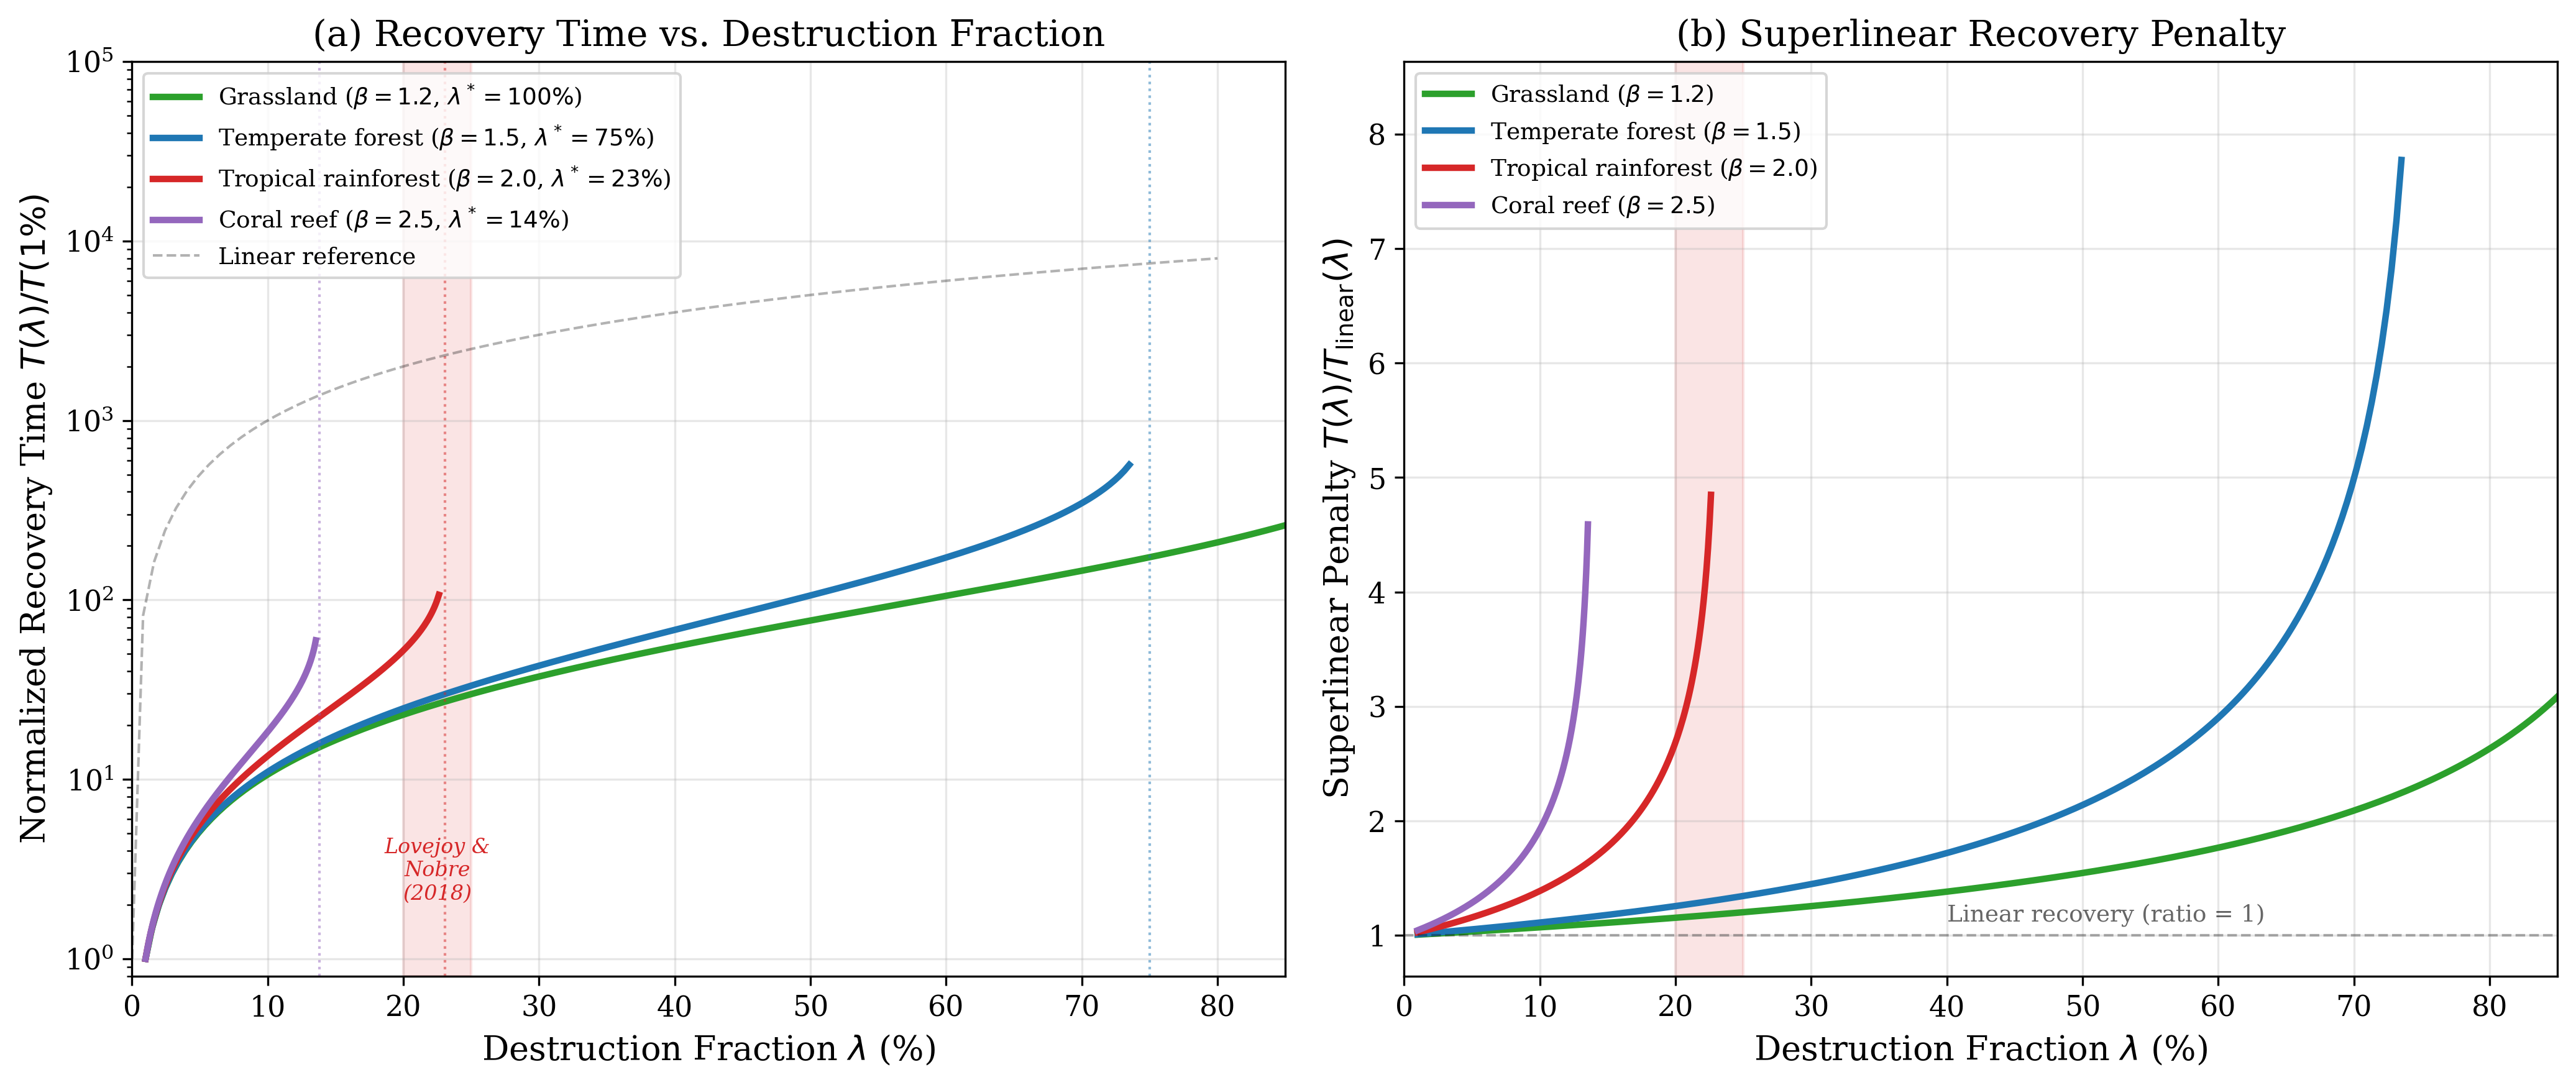
\includegraphics[keepaspectratio,alt={Figure 8: Superlinear Recovery Time. (a) Normalized recovery time T(\textbackslash lambda)/T(1\textbackslash\%) vs.~destruction fraction \textbackslash lambda for four ecosystem types with different \textbackslash beta values and surplus ratios. Grasslands (\textbackslash beta = 1.2) show approximately linear recovery; tropical rainforests (\textbackslash beta = 2.0) and coral reefs (\textbackslash beta = 2.5) show sharply nonlinear recovery diverging at the tipping threshold \textbackslash lambda\^{}*. The shaded band marks the Lovejoy-Nobre 20-25\% Amazon threshold. (b) Superlinear penalty ratio T(\textbackslash lambda)/T\_\{\textbackslash text\{linear\}\}(\textbackslash lambda): a ratio of 1 indicates linear recovery; values exceeding 1 indicate superlinear time debt. High-\textbackslash beta systems incur steeply increasing time penalties with each additional percent of destruction.}]{fig_recovery_time.png}}
\caption{Figure 8: Superlinear Recovery Time. (a) Normalized recovery
time \(T(\lambda)/T(1\%)\) vs.~destruction fraction \(\lambda\) for four
ecosystem types with different \(\beta\) values and surplus ratios.
Grasslands (\(\beta = 1.2\)) show approximately linear recovery;
tropical rainforests (\(\beta = 2.0\)) and coral reefs (\(\beta = 2.5\))
show sharply nonlinear recovery diverging at the tipping threshold
\(\lambda^*\). The shaded band marks the Lovejoy-Nobre 20-25\% Amazon
threshold. (b) Superlinear penalty ratio
\(T(\lambda)/T_{\text{linear}}(\lambda)\): a ratio of 1 indicates linear
recovery; values exceeding 1 indicate superlinear time debt.
High-\(\beta\) systems incur steeply increasing time penalties with each
additional percent of destruction.}
\end{figure}

\subsubsection{The Conservation Fidelity
Bound}\label{the-conservation-fidelity-bound}

A natural proposal for mitigating destruction is \emph{ex-situ
conservation}: copying the information content of a complex system
(genome databases, seed banks, tissue archives) before allowing the
original to be destroyed. The following result establishes that this
strategy faces a fundamental thermodynamic limitation: the cost of
maintaining functional fidelity in an ex-situ copy converges to the cost
of maintaining the system in situ.

\begin{definition}[Static Information]
\label{def-static-information}

The \textbf{static information} $H_{\text{static}}$ of a complex dissipative structure $S$ is the component of its total functional information consisting of sequence data, molecular blueprints, and structural specifications that can be encoded as a bit string and copied at Landauer cost $W_L = H_{\text{static}} \cdot k_B T \ln 2$. Examples: genome sequences, protein primary structures, morphological descriptions.
\end{definition}

\begin{definition}[Dynamic Information]
\label{def-dynamic-information}

The \textbf{dynamic information} $H_{\text{dynamic}}$ of a complex dissipative structure $S$ is the component of its total functional information consisting of relational and process information that exists only as ongoing interactions within the system and its environment. Examples: protein folding pathways in cellular context, species interaction networks, epigenetic regulatory states, evolutionary trajectories in adaptive landscapes.

The total functional information decomposes as $H_{\text{func}} = H_{\text{static}} + H_{\text{dynamic}}$.
\end{definition}

\begin{proposition}[Conservation Fidelity Bound]
\label{prop-conservation-fidelity-bound}

Let $S$ be a self-maintaining dissipative structure whose maintenance power $\dot{W}_{\text{maintain}}$ is fully covered by self-captured energy ($\dot{W}_{\text{capture}} \geq \dot{W}_{\text{maintain}}$). Assume that maintaining the dynamic information component $H_{\text{dynamic}}$ (Definition~\ref{def-dynamic-information}) at fidelity $\phi \in [0,1]$ requires reproducing fraction $\phi$ of the internal processes that consume $\dot{W}_{\text{maintain}}$ in the original, so that an ex-situ copy at fidelity $\phi$ has dynamic-maintenance power requirement $\dot{W}_{\text{dyn}}(\phi) \geq \phi \cdot \dot{W}_{\text{maintain}}$. Then the external maintenance power required by the ex-situ copy $S'$ satisfies:

$$\dot{W}_{\text{external}}(\phi) \geq \phi \cdot \dot{W}_{\text{maintain}}$$

since the ex-situ copy, removed from its energy-capture environment, cannot self-maintain.

(a) At $\phi = 0$ (static sequence data only): $\dot{W}_{\text{external}} \approx 0$ (storage cost is negligible: a hard drive consumes far less energy than a living ecosystem).

(b) At $\phi = 1$ (perfect functional replication): $\dot{W}_{\text{external}} \geq \dot{W}_{\text{maintain}}$.

(c) Since $S$ in situ requires zero net external energy (it is self-sustaining), the external cost of ex-situ conservation at fidelity $\phi > 0$ strictly exceeds the external cost of in-situ preservation.
\end{proposition}

\begin{proof}
A self-maintaining dissipative structure satisfies $\dot{W}_{\text{capture}} \geq \dot{W}_{\text{maintain}}$ by definition (this is the condition for thermodynamic self-sustainability). The net external cost of in-situ preservation is therefore $\dot{W}_{\text{in-situ}}^{\text{ext}} = \max(0,\, \dot{W}_{\text{maintain}} - \dot{W}_{\text{capture}}) = 0$.

For an ex-situ copy at fidelity $\phi$: by hypothesis, maintaining the dynamic information at fidelity $\phi$ requires reproducing fraction $\phi$ of the internal processes that consume $\dot{W}_{\text{maintain}}$ in the original. Since the copy is removed from the self-capture environment, $\dot{W}_{\text{capture}}^{S'} \approx 0$ for a synthetic archive; therefore all maintenance energy must be supplied externally, giving $\dot{W}_{\text{external}}(\phi) \geq \phi \cdot \dot{W}_{\text{maintain}}$. Parts (a) and (b) follow by substitution. For (c): for any $\phi > 0$, $\dot{W}_{\text{external}}(\phi) \geq \phi \cdot \dot{W}_{\text{maintain}} > 0 = \dot{W}_{\text{in-situ}}^{\text{ext}}$, a strict inequality.
\end{proof}

\begin{corollary}[Generative Loss of Ex-Situ Copies]
\label{cor-generative-loss-ex-situ}

An ex-situ copy at fidelity $\phi < 1$ also forfeits a fraction $(1 - \phi)$ of the original system's generative information stream. Under rate-stock coupling, the capitalized value of this lost stream is:

$$\Delta PV_{\text{gen}}(\phi) = \frac{\alpha v \mathcal{N}^\beta}{r}[1 - \phi^\beta]$$

which exceeds $(1-\phi)$ of the total generative value for $\beta > 1$: even small fidelity losses produce disproportionately large generative-value losses.
\end{corollary}

\begin{proof}
The ex-situ copy's effective negentropy is $\phi \mathcal{N}$, giving generative rate $\alpha(\phi\mathcal{N})^\beta = \alpha\phi^\beta\mathcal{N}^\beta$. The loss relative to the original is $\alpha\mathcal{N}^\beta(1 - \phi^\beta)$, capitalized at rate $r$. Since $\phi^\beta < \phi$ for $\phi \in (0,1)$ and $\beta > 1$, we have $1 - \phi^\beta > 1 - \phi$.
\end{proof}

\begin{remark}[Implications for conservation strategy]
\label{rem-conservation-strategy}

Proposition~\ref{prop-conservation-fidelity-bound} and Corollary~\ref{cor-generative-loss-ex-situ} together formalize a principle well understood by conservation biologists: ex-situ archives (seed banks, genome databases, frozen tissue repositories) are complements to in-situ habitat preservation, not substitutes for it. A genome sequence ($\phi \approx 0$: static information only) is cheap to store but preserves almost none of the system's dynamic or generative value. Maintaining a living population in a controlled environment ($\phi$ moderate) recovers some dynamic information but at non-trivial ongoing cost. Only full in-situ preservation ($\phi = 1$) captures the complete generative stream at zero net external cost, precisely because the self-sustaining dissipative structure pays its own maintenance from captured environmental energy. These results provide a thermodynamic basis for the precautionary principle in conservation: when in doubt, preserve in situ.
\end{remark}

\subsection{Synthesis: The Cross-Scale Sustainability
Theorem}\label{synthesis-the-cross-scale-sustainability-theorem}

\subsubsection{Synthesizing the Bounds}\label{synthesizing-the-bounds}

Combining the results of this section:

\begin{theorem}[Cross-Scale Sustainability Theorem]
\label{thm-negentropy-defense}

For a complex dissipative structure, three independent thermodynamic bounds establish that the costs of destruction exceed its yields:

(i) \textbf{Stock bound:} The accumulated negentropy $\mathcal{N}_{\text{bio}} \sim 10^{29}$ J exceeds the net destruction yield $E_{\text{destroy}} - W_{\text{destroy}} \sim 10^{22}$ J by a factor of $\sim 10^7$ (Theorem~\ref{thm-irrationality-destruction}).

(ii) \textbf{Flow bound:} The biosphere's generative information rate $\dot{\mathcal{I}}_{\text{gen}} > 0$ constitutes a perpetual stream of novel information with present value $PV_{\text{gen}} = \dot{\mathcal{I}}_{\text{gen}} \cdot v / r$, which is permanently lost upon destruction (Theorem~\ref{thm-present-value-generative-info}). Under rate-stock coupling (Proposition~\ref{prop-superlinear-destruction-penalty}), even partial destruction degrades this stream superlinearly.

(iii) \textbf{Friction bound:} Dismantling a distributed adaptive biosphere requires sustained boundary-breaking at cost $W_{\text{destroy}} \geq 10^{18}$ J and injects thermodynamic friction into every connected network, degrading downstream operational efficiency (Theorem~\ref{thm-cascading-friction}).

Two of these three bounds (flow, friction) are independent of how the system's complexity is valued.
\end{theorem}

\begin{proof}
We verify each bound independently.

\textbf{Stock bound:} $E_{\text{destroy}} - W_{\text{destroy}} \approx 10^{22}$ J (Proposition~\ref{prop-minimum-destruction-energy}). The accumulated negentropy lost is $\mathcal{N} \sim 10^{29}$ J (Theorem~\ref{thm-minimum-replication-cost}, Estimate 1). Since $10^{22} \ll 10^{29}$, the energy recovered does not compensate for the information destroyed (Theorem~\ref{thm-irrationality-destruction}). ✓

\textbf{Flow bound:} Destruction eliminates a positive-NPV stream of novel information (Theorem~\ref{thm-present-value-generative-info}). A self-maintaining biosphere captures this stream at zero external cost. ✓

\textbf{Friction bound:} Large-scale destruction injects friction $\Delta\phi = \eta \cdot W_{\text{destroy}}$ (Definition~\ref{def-friction-injection}) with total cascading cost $\eta \cdot W_{\text{destroy}} \cdot M \bar{E} / \epsilon$ over the full recovery period (Theorem~\ref{thm-cascading-friction}), degrading all connected networks (Theorem~\ref{thm-network-adjusted-cooperation}). ✓

By the valuation-independent bounds (§\ref{robustness-valuation-independent-bounds}), the flow and friction bounds are independent of how the system's complexity is valued.
\end{proof}

\subsection{Worked Examples}\label{worked-examples-1}

\subsubsection{Example 1: Single Genome, Random Assembly
vs.~Evolution}\label{example-1-single-genome-random-assembly-vs.-evolution}

\textbf{Question:} What is the probability that random assembly produces
a functional human genome?

\textbf{Setup:} The human genome has
\(\mathcal{I}_{\text{func}} = 6.4 \times 10^8\) functional bits. Each
bit must be correct for the genome to be functional (conservative:
binary choice per position).

\textbf{Probability of random success:}

\[p_{\text{random}} = 2^{-\mathcal{I}_{\text{func}}} = 2^{-6.4 \times 10^8} \approx 10^{-1.93 \times 10^8}\]

\textbf{Expected trials needed:}
\(1/p_{\text{random}} \approx 10^{1.93 \times 10^8}\) trials.

\textbf{Minimum energy per trial} (Landauer bound):
\(\mathcal{I}_{\text{func}} \times k_B T \ln 2 = 6.4 \times 10^8 \times 2.87 \times 10^{-21} = 1.84 \times 10^{-12}\)
J.

\textbf{Total expected minimum energy:}

\[W_{\text{random}} = 10^{1.93 \times 10^8} \times 1.84 \times 10^{-12} \approx 10^{1.93 \times 10^8} \text{ J}\]

For comparison, the observable universe contains approximately
\(10^{69}\) J of energy\citep{Penrose2005}. The random-assembly cost
exceeds the energy content of the observable universe by a factor of
\(\sim 10^{1.93 \times 10^8 - 69} \approx 10^{1.93 \times 10^8}\).
Random assembly of a functional genome is not merely impractical; it is
cosmically impossible.

\textbf{What evolution achieves:} By using selection pressure to retain
favorable mutations incrementally, evolution reduces the search cost
from \(\sim 10^{1.93 \times 10^8}\) J (random) to \(\sim 10^{29}\) J
(the accumulated negentropy of the biosphere). This is evolution's
efficiency \emph{relative to blind random assembly},
\(\sigma_{\text{rand}} \approx 10^{29} / 10^{1.93 \times 10^8} \approx 10^{-1.93 \times 10^8 + 29}\)
--- a different and far smaller quantity than the reconstruction
efficiency \(\sigma \in (0,1]\) of
Definition~\ref{def-search-efficiency-factor}, which takes blind
\emph{evolutionary} search (not random assembly) as its unit and is
floored at \(\sigma_{\min} = 1/\Xi = 10^{-35}\). It illustrates why
evolution, despite appearing ``wasteful,'' is an extraordinarily
efficient search algorithm relative to blind random search.

\subsubsection{Example 2: Accumulated Negentropy vs.~Human Energy
Use}\label{example-2-accumulated-negentropy-vs.-human-energy-use}

\textbf{Question:} How does the biosphere's accumulated negentropy
compare to the scale of human economic activity?

\textbf{Setup:}

{\def\LTcaptype{none} %
\begin{longtable}[]{@{}
  >{\raggedright\arraybackslash}p{(\linewidth - 4\tabcolsep) * \real{0.3333}}
  >{\raggedright\arraybackslash}p{(\linewidth - 4\tabcolsep) * \real{0.3333}}
  >{\raggedright\arraybackslash}p{(\linewidth - 4\tabcolsep) * \real{0.3333}}@{}}
\toprule\noalign{}
\begin{minipage}[b]{\linewidth}\raggedright
Quantity
\end{minipage} & \begin{minipage}[b]{\linewidth}\raggedright
Value
\end{minipage} & \begin{minipage}[b]{\linewidth}\raggedright
Source
\end{minipage} \\
\midrule\noalign{}
\endhead
\bottomrule\noalign{}
\endlastfoot
Biosphere accumulated negentropy \(\mathcal{N}_{\text{bio}}\) &
\(\sim 10^{29}\) J &
§\ref{top-down-solar-energy-captured-by-the-biosphere} \\
Global primary energy consumption (2024) & \(\sim 6 \times 10^{20}\)
J/yr & IEA World Energy Outlook \\
Cumulative human energy use over all of history (\(\sim 10^4\) yrs) &
\(\sim 10^{23}\) J & See note below \\
\end{longtable}
}

\emph{Note on cumulative estimate:} Industrial-era consumption
($\sim$200 years averaging \(\sim 5 \times 10^{12}\) W) contributes
\(\sim 3 \times 10^{22}\) J. Pre-industrial consumption (\(\sim 10^4\)
years at \(\sim 10^{11}\) W) contributes a comparable amount. The sum
lies in the range \(3 \times 10^{22}\) to \(3 \times 10^{23}\) J; we use
\(\sim 10^{23}\) J as a round upper bound.

The biosphere's accumulated negentropy exceeds cumulative human energy
consumption over all of recorded history by a factor of \(\sim 10^6\).
Even if global energy consumption continued at current rates for another
million years, the total (\(\sim 6 \times 10^{26}\) J) would still fall
short of \(\mathcal{N}_{\text{bio}}\) by two orders of magnitude.

\textbf{The search cost is the binding constraint.} The search cost
amplification factor \(\Xi \sim 10^{35}\)
(Definition~\ref{def-search-cost-amplification}) means that the
evolutionary process that discovered \emph{which} configurations are
functional consumed \(10^{35}\) times more energy than the Landauer
minimum for writing the resulting information. Raw energy is not the
bottleneck for replacing biological complexity; the bottleneck is the
search cost of rediscovering \(\sim 10^{15}\) bits of functional
information from a configuration space of size
\(\sim 10^{6.4 \times 10^8}\).

\textbf{Conclusion:} The biosphere's accumulated thermodynamic
investment dwarfs the total energy throughput of human civilization. The
information it encodes, selected over \(4 \times 10^9\) years of
evolutionary search, represents the single most information-dense
structure in the known Solar System.

\subsubsection{Example 3: The Burning-Library
Quantification}\label{example-3-the-burning-library-quantification}

The Burning-Library Ratio (Definition~\ref{def-burning-library-ratio})
quantifies the fraction of a system's accumulated thermodynamic
investment recoverable through destruction. The following worked
examples compute this ratio at two scales: a single ecosystem and the
full biosphere.

\paragraph{The Amazon Rainforest}\label{the-amazon-rainforest}

\textbf{Question:} What fraction of the Amazon's accumulated
thermodynamic value is recovered by converting its biomass to raw
energy?

\textbf{Setup:}

{\def\LTcaptype{none} %
\begin{longtable}[]{@{}
  >{\raggedright\arraybackslash}p{(\linewidth - 4\tabcolsep) * \real{0.3333}}
  >{\raggedright\arraybackslash}p{(\linewidth - 4\tabcolsep) * \real{0.3333}}
  >{\raggedright\arraybackslash}p{(\linewidth - 4\tabcolsep) * \real{0.3333}}@{}}
\toprule\noalign{}
\begin{minipage}[b]{\linewidth}\raggedright
Quantity
\end{minipage} & \begin{minipage}[b]{\linewidth}\raggedright
Value
\end{minipage} & \begin{minipage}[b]{\linewidth}\raggedright
Source
\end{minipage} \\
\midrule\noalign{}
\endhead
\bottomrule\noalign{}
\endlastfoot
Total biomass (above and below-ground) & 86 Pg C &
\citet{Saatchi2007} \\
Dry mass (\(2\times\) carbon conversion) & \(1.72 \times 10^{14}\) kg &
Calculated \\
Calorific value (tropical hardwood) & \(\sim 19\) MJ/kg & Standard
thermodynamic value \\
Amazon basin GPP & \(\sim 20\) Pg C/yr &
\citet{SciencePanelAmazon2021} \\
Global terrestrial GPP & \(\sim 120\) Pg C/yr & \citet{Beer2010} \\
\end{longtable}
}

\textbf{Extractable energy.} The Amazon basin contains approximately 86
Pg C of total biomass \citep{Saatchi2007}, corresponding to
\(\sim 1.72 \times 10^{14}\) kg of dry mass. At a calorific value of
\(\sim 19\) MJ/kg for tropical hardwood:

\[E_{\text{destroy}} \approx 1.72 \times 10^{14} \times 1.9 \times 10^{7} \approx 3.3 \times 10^{21} \text{ J}\]

\textbf{Accumulated negentropy (lower bound).} The Amazon contributes
approximately 16\% of global terrestrial gross primary production
(\(\sim 20\) out of \(\sim 120\) Pg C/yr;
\citet{SciencePanelAmazon2021}; \citet{Beer2010}). Allocating biosphere
accumulated negentropy
(§\ref{top-down-solar-energy-captured-by-the-biosphere}) in proportion
to productivity share:

\[\mathcal{N}_{\text{Amazon}} \sim \frac{P_{\text{GPP, Amazon}}}{P_{\text{GPP, global}}} \cdot \mathcal{N}_{\text{bio}} \approx 0.16 \times 10^{29} \sim 10^{28} \text{ J}\]

This is a lower bound: the Amazon is disproportionately biodiverse
relative to its productivity share, and the underlying biosphere
estimate uses a conservative ordering efficiency
(\(\eta_{\text{order}} = 0.01\)). The modern Amazon basin has sustained
continuous tropical forest cover for at least \(5.5 \times 10^7\) years
\citep{Morley2000}, but the lineages it shelters inherit metabolic and
informational complexity accumulated over the full
\(4 \times 10^9\)-year history of life.

\textbf{Burning-Library Ratio:}

\[\mathcal{R}_{\text{BL}} = \frac{E_{\text{destroy}}}{\mathcal{N}_{\text{Amazon}}} = \frac{3.3 \times 10^{21}}{10^{28}} \approx 3 \times 10^{-7}\]

\textbf{Result:} Complete destruction of the Amazon rainforest recovers
approximately three ten-millionths of its accumulated thermodynamic
value as raw energy. The remaining 99.99997\% represents information and
structural complexity that destruction dissipates irreversibly. This
ratio is comparable to the biosphere-scale result computed below.

\paragraph{Earth's Biosphere}\label{earths-biosphere}

\textbf{Question:} What fraction of the biosphere's value is recovered
by harvesting its raw chemical energy?

\textbf{Setup:} - Extractable chemical energy:
\(E_{\text{destroy}} \sim 10^{22}\) J (§\ref{the-destruction-yield}) -
Accumulated negentropy: \(\mathcal{N}_{\text{bio}} \sim 10^{29}\) J
(§\ref{top-down-solar-energy-captured-by-the-biosphere}) - Generative
information value (100-year horizon, \(r = 0.05\)):
\(PV_{\text{gen}} = \dot{\mathcal{I}}_{\text{gen}} \cdot v / r\)

Estimating the generative rate: global speciation rate \(\sim 10^{-3}\)
to \(10^{-1}\) new species per year across all taxa, each contributing
\(\sim 10^7\) unique bits, giving
\(\dot{\mathcal{I}}_{\text{gen}} \sim 10^4\) to \(10^6\) bits/yr. At
\(v \sim 10^9\) J/bit (order-of-magnitude cost of producing one
functional bit through evolution, from
\(\mathcal{N}_{\text{bio}} / H_{\text{biosphere}} \approx 10^{29}/10^{15} = 10^{14}\)
J/bit, however we use \(v \sim 10^9\) as a conservative valuation
reflecting diminishing marginal returns):

\[PV_{\text{gen}} \sim \frac{10^6 \times 10^9}{0.05} = 2 \times 10^{16} \text{ J}\]

\textbf{Total preservation value:}

\[V_{\text{preserve}} = \mathcal{N}_{\text{bio}} + PV_{\text{gen}} \approx 10^{29} + 10^{16} \approx 10^{29} \text{ J}\]

(The stock term dominates.)

\textbf{Fraction recovered by destruction:}

\[\frac{E_{\text{destroy}}}{V_{\text{preserve}}} = \frac{10^{22}}{10^{29}} = 10^{-7}\]

\textbf{Result:} The extractable raw energy from the biosphere is one
ten-millionth of its total thermodynamic value. The remaining 99.99999\%
of the accumulated investment has no recoverable energy equivalent.

\subsection{Discussion}\label{discussion-2}

\subsubsection{Physical Interpretation}\label{physical-interpretation-3}

The accumulated negentropy framework provides a thermodynamic accounting
of irreversibility in complex systems. The central result, the
Burning-Library Ratio of \(\sim 10^{-7}\)
(Corollary~\ref{cor-burning-library-inequality}), quantifies the gap
between the energy extractable through destruction and the thermodynamic
investment embodied in biological complexity. This is not a subjective
valuation but a physical accounting: the work required to recreate the
information content exceeds the energy recoverable from destruction by
seven orders of magnitude.

The biosphere estimate of \(\mathcal{N}_{\text{bio}} \sim 10^{29}\) J is
cross-validated by an independent calculation using Chaisson's energy
rate density measurements \citep{Chaisson2011} weighted by Bar-On et
al.'s biomass fractions \citep{BarOn2018}, which yields
\(\sim 7 \times 10^{28}\) J
(§\ref{cross-validation-via-energy-rate-density}). Agreement within a
factor of 1.36 between two methodologically independent routes (solar
flux accounting vs.~organism-level energy budgets) provides robust
confirmation of the order of magnitude.

The result is robust to substantial parameter uncertainty
(\ref{rem-order-of-magnitude}). Even if the accumulated negentropy
estimate is wrong by a factor of \(10^3\), the gap remains four orders
of magnitude. The Burning-Library Ratio provides a physically grounded,
order-of-magnitude ``floor'' on the value of complex systems.

The cost-benefit bound (Theorem~\ref{thm-irrationality-destruction}) and
the cross-scale sustainability theorem
(Theorem~\ref{thm-negentropy-defense}) together establish three
independent thermodynamic bounds on the costs of destruction: stock
value, generative information flow, and network friction costs.
Crucially, two of these three bounds are valuation-independent
(§\ref{robustness-valuation-independent-bounds}): the flow and friction
bounds impose costs regardless of the purpose of the extraction. The
convergence of these independent bounds makes the conclusion robust to
failure of any single bound: even if one metric were invalidated, the
remaining two suffice.

The rate-stock coupling framework (§\ref{the-generative-data-argument})
adds dynamic consequences to the static Burning-Library accounting. The
front-loaded cost structure
(Proposition~\ref{prop-portfolio-destruction-ordering}) shows that the
marginal cost of destruction is highest for the first increment,
creating a strong thermodynamic disincentive against initiating any
damage. Recovery from destruction is superlinear in the damage fraction
(Proposition~\ref{prop-superlinear-recovery-time}): doubling the
destruction more than doubles the recovery time, and recovery diverges
to infinity at the tipping threshold. The conservation fidelity bound
(Proposition~\ref{prop-conservation-fidelity-bound}) establishes that
ex-situ archives (seed banks, genome databases) are complements to, not
substitutes for, in-situ preservation, because the external cost of
maintaining dynamic information at high fidelity converges to the
in-situ maintenance cost while the original self-maintains at zero
external cost.

\subsubsection{Testable Predictions}\label{testable-predictions-2}

These results generate falsifiable predictions:

{\def\LTcaptype{none} %
\begin{longtable}[]{@{}
  >{\raggedright\arraybackslash}p{(\linewidth - 4\tabcolsep) * \real{0.3333}}
  >{\raggedright\arraybackslash}p{(\linewidth - 4\tabcolsep) * \real{0.3333}}
  >{\raggedright\arraybackslash}p{(\linewidth - 4\tabcolsep) * \real{0.3333}}@{}}
\toprule\noalign{}
\begin{minipage}[b]{\linewidth}\raggedright
Prediction
\end{minipage} & \begin{minipage}[b]{\linewidth}\raggedright
Source
\end{minipage} & \begin{minipage}[b]{\linewidth}\raggedright
Falsified If\ldots{}
\end{minipage} \\
\midrule\noalign{}
\endhead
\bottomrule\noalign{}
\endlastfoot
Biosphere accumulated negentropy \(\sim 10^{29}\) J &
Definition~\ref{def-accumulated-negentropy},
§\ref{biosphere-estimation-the-4-billion-year-ledger} estimates &
Independent estimates of ordering work over geological time yield
\(< 10^{26}\) J or \(> 10^{32}\) J \\
Cross-validation via Chaisson's \(\Phi_m\) yields
\(\sim 7 \times 10^{28}\) J &
§\ref{cross-validation-via-energy-rate-density}, \citep{Chaisson2011} &
Organism-level energy budgets yield biosphere ordering rate inconsistent
with GPP by more than an order of magnitude \\
Burning-Library Ratio \(\sim 10^{-7}\) for Earth's biosphere &
Corollary~\ref{cor-burning-library-inequality} & Extractable chemical
energy from biomass exceeds \(10^{26}\) J, or accumulated negentropy is
below \(10^{26}\) J \\
Generative information rate \(\dot{\mathcal{I}}_{\text{gen}} > 0\) for
evolving ecosystems & Theorem~\ref{thm-present-value-generative-info} &
An active biosphere produces no novel functional information over
measurable timescales (no speciation, no adaptive mutations) \\
Replication cost \(\geq \mathcal{N}_{\text{bio}}\) for blind-search
rebuilding & Theorem~\ref{thm-minimum-replication-cost} & A demonstrated
method reconstructs an equivalently complex information-bearing system
at energy cost \(\ll \mathcal{N}\) \\
Superlinear generative-value loss under partial destruction &
Proposition~\ref{prop-superlinear-destruction-penalty} & Empirical
measurement of speciation or adaptive mutation rates in ecosystems of
varying complexity shows a linear (not superlinear) relationship between
complexity and generative rate \\
Tipping threshold \(\lambda^*\) consistent with Lovejoy-Nobre 20-25\% &
Proposition~\ref{prop-negentropy-tipping-point},
\citep{LovejoyNobre2018} & Calibrated \(\beta\) and \(R\) for the Amazon
yield \(\lambda^*\) outside the 15-30\% range, or grasslands show
comparable threshold fragility \\
Recovery time convex in destruction fraction, diverging at \(\lambda^*\)
& Proposition~\ref{prop-superlinear-recovery-time} & Ecosystem recovery
timescales scale linearly with damage fraction, or severely damaged
high-\(\beta\) systems recover as fast as low-\(\beta\) systems \\
Ex-situ conservation cost converges to in-situ cost at high fidelity &
Proposition~\ref{prop-conservation-fidelity-bound} & Maintaining a
functionally complete ex-situ replica of a complex ecosystem at
substantially lower energy cost than the original \\
\end{longtable}
}

\subsubsection{Limitations}\label{limitations-2}

The accumulated negentropy results depend on order-of-magnitude
estimates that are robust to factor-of-10 uncertainties but sensitive to
definitions of ``functional information'' (see
\ref{rem-order-of-magnitude}). The distinction between total Shannon
entropy and functionally relevant information remains an active research
question. The Burning-Library Ratio's seven-order-of-magnitude gap
provides substantial margin against this definitional uncertainty: even
factor-of-\(10^3\) errors in the accumulated negentropy estimate leave a
four-order-of-magnitude gap.

The search cost amplification factor (\(\Xi \sim 10^{35}\)) assumes
blind search as the baseline. Directed search methods (evolution,
machine learning) reduce this, but even optimistic estimates leave the
amplification at \(\sim 10^{10}\) to \(10^{20}\).

The rate-stock coupling (Definition~\ref{def-rate-stock-coupling},
Proposition~\ref{prop-superlinear-destruction-penalty}) assumes a
power-law functional form
\(\dot{\mathcal{I}}_{\text{gen}} = \alpha \mathcal{N}^\beta\) with
\(\beta > 1\). The superlinearity is motivated by the combinatorial
argument (more components yield superlinearly more interaction
possibilities), but the exponent \(\beta\) has not been directly
measured. However, the tipping-point prediction
(Proposition~\ref{prop-negentropy-tipping-point}) provides an indirect
calibration: the observed 20-25\% deforestation threshold for the Amazon
\citep{LovejoyNobre2018} implies a generative surplus ratio
\(R \approx 1.25\)-\(1.33\), and the contrast between
threshold-dominated tropical forests and resilient grasslands is
consistent with \(\beta \approx 2\) for the former and
\(\beta \approx 1.2\) for the latter. Direct ecological measurement of
the relationship between ecosystem complexity and information generation
rate would test the superlinearity assumption and constrain \(\beta\);
the analysis predicts that this relationship is steepest for
species-rich systems with dense interaction networks.

\textbf{Scope.} The results apply to any complex dissipative system
whose information content was produced by an extended search process
(evolutionary, developmental, or cultural). The biosphere estimation in
§\ref{biosphere-estimation-the-4-billion-year-ledger} uses
Earth-specific parameters, but the formal results
(Theorem~\ref{thm-irrationality-destruction},
Theorem~\ref{thm-negentropy-defense}) hold for any system satisfying the
assumptions of §\ref{model-and-formal-setup}. This analysis does not
address the \emph{distribution} of value within the biosphere (whether
individual species or ecosystems are equally irreplaceable); such
distributional questions require finer-grained estimates of
per-subsystem accumulated negentropy.

\subsubsection{Applications}\label{applications-2}

\textbf{Conservation economics.} The Burning-Library Ratio provides a
computable standard for preservation policy: the thermodynamic cost of
replacing a destroyed ecosystem can be compared against the economic
value of the resources extracted. For any ecosystem with accumulated
negentropy \(\mathcal{N}\) and extractable resource value
\(E_{\text{extract}}\), the ratio \(E_{\text{extract}} / \mathcal{N}\)
quantifies the fraction of accumulated value recoverable through
destruction. Where this ratio is small (as it is for all biologically
complex systems), destruction is a net-negative trade even before
accounting for ecosystem services. In
§\ref{example-3-the-burning-library-quantification}, the ratio has been
computed for the Amazon rainforest
(\(\mathcal{R}_{\text{BL}} \sim 10^{-7}\)) in addition to the full
biosphere, confirming that the seven-order-of-magnitude gap persists at
the individual ecosystem scale.

\textbf{Cultural and institutional capital.} The analysis applies to any
complex dissipative system whose information content was produced by
extended search (§\ref{model-and-formal-setup}). Cultural systems
(languages, legal traditions, indigenous knowledge) are plausible
candidates: their information content was refined over generations
through iterative selection, and they are maintained through continued
use. Whether the Burning-Library Ratio and rate-stock coupling results
transfer quantitatively to such systems is an open empirical question,
but the formal structure suggests that the asymmetry between destruction
cost and reconstruction cost may be similarly severe wherever the
underlying information was produced by extended trial-and-error rather
than deliberate design.

\textbf{Information thermodynamics.} The search cost amplification
factor \(\Xi\) (Definition~\ref{def-search-cost-amplification})
quantifies the gap between the Landauer floor and the actual cost of
producing functional information through evolutionary search. This
quantity is of independent interest in information thermodynamics, since
it measures the computational work embodied in a specific
information-bearing configuration, a concept with potential applications
in quantifying the value of databases, cultural knowledge, and other
complex information systems.

\subsubsection{Future Work}\label{future-work-2}

\textbf{Sub-biosphere calibration.} Developing detailed estimates of
\(\mathcal{N}(T)\) for ecosystems at multiple scales (individual
organisms, local ecosystems, regional biomes) would empirically validate
the analysis and provide calibration data for the Burning-Library Ratio
at sub-biosphere scales. Genome-level validation of the information
density hierarchy (Definition~\ref{def-information-density},
Definition~\ref{def-specific-information-density}) against molecular
evolution data would test the bottom-up estimation methodology.

\textbf{Rate-stock coupling measurement.} Direct empirical calibration
of the rate-stock coupling exponent \(\beta\)
(Definition~\ref{def-rate-stock-coupling}) from comparative data on
speciation rates and ecosystem complexity would provide a quantitative
test of the superlinearity assumption. The tipping-point observations in
§\ref{the-generative-data-argument} provide indirect constraints
(\(\beta \approx 2\) for tropical forests, \(\beta \approx 1.2\) for
grasslands), but systematic measurement across diverse system types is
needed.

\textbf{Independent cross-validation.} Extending the Chaisson
cross-validation (§\ref{cross-validation-via-energy-rate-density}) to
include independent estimates from geochemistry and population genetics
would further constrain the biosphere negentropy estimate.

\textbf{Dynamic negentropy accumulation in production networks.}
Accumulated negentropy is defined here as a stock. A dynamic extension
to production networks would formalize the \emph{flow} that builds it:
integrated net production over evolutionary time, constrained by
thermodynamic admissibility. Recovery from collapse would acquire a
formal criterion (the spectral radius of the remaining production
network must remain below one and the Hawkins-Simon condition must hold
on the residual input-output matrix). The Burning-Library Ratio would
become the static limit of a dynamic irreplaceability result.

\textbf{Conditional replacement cost.} The blind search replication cost
(Theorem~\ref{thm-minimum-replication-cost}) assumes reconstruction from
zero prior information, yielding the amplification factor
\(\Xi \sim 10^{35}\). When phylogenetic or informational neighbors of
the destroyed system survive, they provide a template that reduces the
effective search space. A conditional replacement cost
\(\Xi_{\text{eff}}\), discounted by the mutual information between the
destroyed system and the best surviving template, would formalize this
reduction:
\(\Xi_{\text{eff}} = \Xi \cdot 2^{-I(\text{destroyed};\text{template})}\).
For closely related species sharing $>$95\% genomic identity, the
discount could span tens of orders of magnitude. The blind search bound
remains tight only when the destroyed system is truly unique (no close
relatives, no archived information).

\subsection{Conclusion}\label{conclusion-2}

We have defined accumulated negentropy as the integrated thermodynamic
work embodied in complex dissipative structures and computed the
Burning-Library Ratio at biosphere scale: the fraction of accumulated
value recoverable through destruction. For Earth's biosphere, this ratio
is approximately \(10^{-7}\), a gap of seven orders of magnitude that is
robust to substantial parameter uncertainty and cross-validated within a
factor of 1.36 by independent energy rate density measurements
(§\ref{cross-validation-via-energy-rate-density}). Living systems
generate information at a positive rate whose present value is
unbounded; under the rate-stock coupling formalized here, even partial
destruction incurs a superlinear penalty on future information
production.

The dynamic consequences of rate-stock coupling extend the static
Burning-Library accounting. Complex systems with high coupling exponents
(\(\beta \gg 1\)) exhibit tipping-point fragility: the Amazon's 20-25\%
deforestation threshold \citep{LovejoyNobre2018} is consistent with the
predicted tipping fraction \(\lambda^*\) for a system operating
$\sim$25-33\% above its maintenance threshold. Recovery from
sub-threshold damage is superlinear in the damage fraction, explaining
why grasslands (\(\beta \approx 1.2\)) recover in years while tropical
forests (\(\beta \approx 2\)) require centuries, if they recover at all.
The front-loaded cost structure of destruction means that an intact
ecosystem's first increment of damage is the most expensive. Ex-situ
conservation archives capture only static information; maintaining
dynamic fidelity converges in cost to maintaining the original system,
while the original self-maintains at zero external cost.

Both thermodynamic bounds beyond the stock bound are
valuation-independent (§\ref{robustness-valuation-independent-bounds}).
Together, these results establish computable, energy-denominated
sustainability limits for any complex dissipative structure whose
information content was produced by extended search.

These results require only Landauer's principle and basic
thermodynamics. They provide the irreplaceability component of the
multi-agent cooperation models developed in \emph{Necessary Constraints}
Appendix~\ref{app-I} and \emph{Thermodynamic Friction}
Appendix~\ref{app-IV}. The strategic entropy injection analysis
Appendix~\ref{app-II} addresses information corruption costs at the
agent-to-agent level; the present paper extends the
information-theoretic analysis to the cross-scale level, quantifying the
irreplaceability of the complex structures that cooperative networks
produce and maintain.

\section{Thermodynamic Friction (Paper TC-IV)}\label{app-IV}

\emph{We quantify the energy cost of adversarial resource competition
between self-maintaining open thermodynamic systems. Boundary
constraints are required for multi-agent resource allocation; we model
what happens when those constraints are violated. Using Tullock contest
theory and a boundary-integrity damage model, we prove that
unconstrained conflict is a net-negative thermodynamic outcome: under
realistic physical parameters, the total energy dissipated by conflict,
including contest expenditure, boundary damage, and thermodynamically
irreversible repair costs, exceeds the value of the contested resource.
We derive explicit Nash equilibrium investments and damage functions for
both symmetric and asymmetric contests, showing that contest dissipation
approaches the full resource value as the number of contestants grows.
Extending the analysis to cooperative networks, we prove that a single
constraint violation cascades through the network, with illustrative
amplification ratios on the order of \(10^3\) to \(10^4\) under modest
network parameters, because trust recovery is gradual while trust
destruction is instantaneous. Cooperation strictly dominates conflict
for all physically realizable friction parameters, providing the
energy-denominated cost structure that enters the game-theoretic payoff
matrices of the subsequent paper in this series.}

\subsection{Introduction}\label{introduction-4}

\emph{Necessary Constraints} Appendix~\ref{app-I} proves that mutual
boundary constraints are necessary for the persistence of multiple
agents in a shared, finite-resource environment. Removing these
constraints leads to resource collision and conflict. This paper
quantifies the thermodynamic cost of that conflict.

When agents compete for a contested resource without cooperative
constraints, the interaction takes the form of a contest: each agent
expends energy to increase its probability of capturing the resource,
and the contest itself dissipates energy that neither agent recovers. We
model this using Tullock contest theory \citep{Tullock1980} with
physical parameters (boundary integrity, damage fractions, repair
multipliers) and prove that the total energy cost of conflict exceeds
the value of the contested resource under realistic conditions ---
destructive boundary damage between two agents, or any positive damage
among three or more.

The specific contributions of this paper are:

\begin{enumerate}
\def\labelenumi{\arabic{enumi}.}
\item
  \textbf{Contest equilibria} (Proposition~\ref{prop-symmetric-contest},
  Proposition~\ref{prop-asymmetric-contest}). We derive the symmetric
  and asymmetric Nash equilibria of the resource contest, showing that
  both agents expend energy proportional to the resource value, and that
  total contest dissipation approaches the full resource value as the
  number of contestants grows (Theorem~\ref{thm-dissipation-scaling}).
\item
  \textbf{Net-negative conflict}
  (Theorem~\ref{thm-net-negative-conflict}). We define the friction
  multiplier
  \(\Phi = 1 + \kappa(\psi^{\text{off}} + \psi^{\text{def}})\)
  incorporating contest expenditure, boundary damage, and
  thermodynamically irreversible repair costs, and prove that the total
  energy dissipated by conflict exceeds the value of the contested
  resource once boundary damage is sufficiently destructive
  (\(\kappa\psi > 1\)) or three or more agents contest it.
\item
  \textbf{Cooperation dominance}
  (Theorem~\ref{thm-cooperation-dominance}). We prove that the
  cooperative regime strictly dominates the conflict regime for all
  physically realizable friction parameters, providing the energy-cost
  foundation for the game-theoretic equilibrium results of
  \emph{Cooperative Equilibrium} Appendix~\ref{app-V}.
\item
  \textbf{Network cascading} (Theorem~\ref{thm-cascading-friction}). We
  prove that a single constraint violation in a cooperative network
  injects friction that degrades all future interactions, with
  illustrative amplification ratios of roughly \(10^3\) to \(10^4\)
  under modest network parameters, formalizing the asymmetry between
  trust destruction and trust recovery.
\end{enumerate}

All formal results are stated as numbered theorems with full proofs,
denominated in energy units, and computationally verified.

The paper proceeds as follows: model and contest framework, boundary
integrity, contest equilibria and full cost of conflict, the
net-negative theorem, cooperative versus conflict regimes, cascading
network effects, the interaction cost function, worked examples,
decisive contests and escalation dynamics, and discussion.

\subsubsection{Related Work}\label{related-work-4}

The mathematical machinery of this work (contest theory, Nash
equilibria, and boundary-damage models) draws on established literatures
in conflict economics, non-equilibrium thermodynamics, and network
theory. Our contribution is the synthesis: connecting contest-theoretic
dissipation to thermodynamic boundary costs and network friction to
derive a unified, energy-denominated cost function for adversarial
interaction.

\textbf{Contest theory and conflict economics.} \citet{Tullock1980}
introduced the ratio-form contest success function in the context of
rent-seeking, showing that competitions for rents dissipate a
substantial fraction of the rent's value. \citet{Skaperdas1996}
axiomatized the Tullock contest success function, proving it is the
unique function satisfying homogeneity, monotonicity, and independence
from irrelevant alternatives. \citet{Hirshleifer1991} analyzed conflict
as an economic activity, modeling the ``technology of conflict'' through
contest production functions and demonstrating that resources devoted to
fighting are pure waste from the system's perspective.
\citet{GarfinkelSkaperdas2012} provide a comprehensive treatment of the
economics of peace and conflict, synthesizing decades of work on arms
races, territorial disputes, and the welfare costs of insecurity.
\citet{Konrad2009} surveys the theory of contests more broadly, covering
multi-player, multi-stage, and asymmetric extensions. This literature
establishes that contest dissipation is a pervasive feature of
competitive interaction, but treats payoffs in dimensionless utility
units and does not connect dissipation to physical energy budgets. Our
framework denominates all contest payoffs in energy units and augments
the standard Tullock model with boundary-damage and repair costs derived
from thermodynamic principles.

\textbf{Non-equilibrium thermodynamics and boundary maintenance.} The
physical model of agents as open thermodynamic systems maintaining
low-entropy internal states draws on \citet{Schrodinger1944}, who
identified that living systems persist by importing free energy and
exporting entropy. \citet{Prigogine1978} demonstrated that systems far
from equilibrium can spontaneously generate ordered structures through
symmetry-breaking instabilities, but did not formalize the boundaries
that maintain organized entities as distinct agents or the energetic
cost of boundary breaches. \citet{England2013} derived a
statistical-mechanical lower bound on heat production during
self-replication. \citet{Friston2013} formalized persistence via Markov
blankets under the Free Energy Principle, addressing the single-agent
problem of what one entity does to maintain itself. \citet{Maturana1980}
described the operational closure of self-producing systems
(autopoiesis), the topology of self-maintenance that our boundary
integrity parameter \(B_i\) quantifies energetically. The thermodynamic
tradition establishes that boundary maintenance is energetically costly
and that entropy increase is thermodynamically irreversible; our
contribution is proving that boundary damage from conflict incurs repair
costs strictly exceeding the original damage (a consequence of the
Second Law), making conflict a thermodynamically amplified loss.

\textbf{Network effects and transaction costs.} The cascading friction
analysis draws on network theory and transaction cost economics.
\citet{Jackson2008} develops the theory of network formation and
stability, showing that network structure affects the efficiency of
economic exchange. \citet{Ostrom1990} documented how communities develop
institutional constraint systems (monitoring, graduated sanctions,
conflict resolution mechanisms) to manage shared resources, institutions
whose overhead costs correspond to our network friction coefficient
\(\phi\). The ecological economics tradition
\citep{Lotka1922, GeorgescuRoegen1971} recognized that energy is the
fundamental currency of biological and economic activity, and that the
Second Law imposes irreversible costs on all transformations
\citep{GeorgescuRoegen1979}. Our contribution is quantifying the
cascading cost of trust violations across cooperative networks and
proving that the network-level damage exceeds the direct bilateral cost
by orders of magnitude.

\subsection{Model}\label{model-2}

\subsubsection{Agents and Resources}\label{agents-and-resources}

We consider \(N \geq 2\) agents sharing an environment with \(n\)
resource dimensions and finite endowment
\(\mathbf{R} = (R_1, \ldots, R_n) \in \mathbb{R}_{>0}^n\). Each agent
\(i\) is an open thermodynamic system maintaining a boundary between its
internal low-entropy state and the external environment. Agent \(i\)
selects a strategy vector \(\mathbf{x}_i \in \mathbb{R}_{\geq 0}^n\),
and the physically realizable joint strategy must satisfy resource
conservation: \(\sum_{i=1}^N x_{ij} \leq R_j\) for all \(j\).

Each agent's utility function \(U_i(\mathbf{x}_i)\) satisfies the
regularity conditions of \emph{Necessary Constraints}
Appendix~\ref{app-I}: twice continuously differentiable, strictly
concave, monotonically increasing at the origin, and coercive. Under
these conditions, each agent has a unique unconstrained optimum
\(\mathbf{x}_i^{\circ}\). When \(N\) meets the collision threshold for
at least one resource, the aggregate unconstrained demand exceeds supply
(\(\sum_i x_{ij}^{\circ} > R_j\)), and no feasible joint allocation can
simultaneously satisfy all agents' unconstrained optima.

\emph{Necessary Constraints} Appendix~\ref{app-I} proves that boundary
constraints are necessary for feasible allocation in this setting. This
paper addresses the complementary question: what is the energetic cost
when those constraints are absent and the resulting collision is
resolved by direct resource competition?

\subsubsection{Boundary Integrity}\label{boundary-integrity}

Each agent \(i\) maintains a boundary characterized by its integrity
\(B_i > 0\), measured in energy units, representing the total energetic
investment in maintaining the separation between the agent's internal
low-entropy state and the external environment. Maintaining boundary
integrity against environmental entropy requires continuous work
\(C_{\text{maintain},i} = \gamma_i B_i\), where \(\gamma_i > 0\) is the
entropy leakage rate. This is the baseline metabolic cost of
persistence, independent of any external threat.

When an external agent breaches agent \(i\)'s boundary, the work
required scales with the boundary's integrity: full breach requires work
equal to \(B_i\). The specific resistance profile (uniform, hardening,
or shell) affects only the dynamics of partial breach, not the total
cost.

\subsubsection{Contest Framework}\label{contest-framework}

When two or more agents claim the same resource unit and no constraint
directs the allocation, the resource is resolved by a contest: each
agent invests energy to increase its probability of winning. We adopt
the Tullock contest success function \citep{Tullock1980, Skaperdas1996}:

\[p_A(e_A, e_B) = \frac{\sigma_A \, e_A^r}{\sigma_A \, e_A^r + \sigma_B \, e_B^r}\]

where \(e_i \geq 0\) is agent \(i\)'s contest investment (energy
diverted from productive use into conflict), \(\sigma_i > 0\) is
conflict effectiveness, and \(r > 0\) is the decisiveness parameter.
This is the unique contest success function satisfying homogeneity,
monotonicity, and independence from irrelevant alternatives
\citep{Skaperdas1996}.

Beyond the direct contest expenditure, conflict inflicts boundary damage
on both parties (offensive self-damage from diverting resources,
defensive damage from the opponent's attack), and repairing that damage
is thermodynamically more expensive than the original maintenance cost,
a direct consequence of the Second Law. The friction multiplier \(\Phi\)
captures the total cost amplification from these combined effects.

\subsection{The Boundary Integrity
Model}\label{the-boundary-integrity-model}

\subsubsection{Boundary as an Energetic
Structure}\label{boundary-as-an-energetic-structure}

Each agent \(i\) maintains a \textbf{boundary} (Markov blanket in
statistical physics; cell membrane in biology; legal/military defense in
sociology) characterized by its \textbf{integrity}:

\begin{definition}[Boundary Integrity]
\label{def-boundary-integrity}

Agent $i$'s boundary integrity is a scalar $B_i > 0$ measured in energy units, representing the total energetic investment in maintaining the boundary between the agent's internal low-entropy state and the external environment.
\end{definition}

\textbf{Physical interpretation:} \(B_i\) is the stored energy in the
agent's defensive infrastructure (the immune system, the cell wall, the
military budget, the information-security apparatus). A higher \(B_i\)
means a more robust boundary that is costlier to breach.

\subsubsection{Boundary Maintenance
Cost}\label{boundary-maintenance-cost}

Maintaining boundary integrity against environmental entropy requires
continuous work:

\[C_{\text{maintain},i} = \gamma_i \cdot B_i\]

where \(\gamma_i > 0\) is the \textbf{entropy leakage rate}, the rate at
which the boundary degrades without active maintenance. This is the
baseline metabolic cost of persistence (maintaining identity),
independent of any external threat.

\subsubsection{Boundary Resistance
Function}\label{boundary-resistance-function}

When an external agent attempts to breach agent \(i\)'s boundary, the
boundary exerts a \textbf{resistance} that the attacker must overcome.
We model this as a force-displacement relationship:

\begin{definition}[Boundary Resistance]
\label{def-boundary-resistance}

The work required to breach agent $i$'s boundary to depth $d \in [0, 1]$ (where $d = 0$ is the exterior and $d = 1$ is full breach) is:

$$W_{\text{breach}}(d) = \int_0^d F_i(s) \, ds$$

where $F_i(s) = B_i \cdot f(s)$ is the resistance force and $f : [0, 1] \to \mathbb{R}_{> 0}$ is a normalized resistance profile with $\int_0^1 f(s) \, ds = 1$.
\end{definition}

The full breach cost is:

\[W_{\text{breach}}(1) = B_i \cdot \int_0^1 f(s) \, ds = B_i\]

That is, fully breaching agent \(i\)'s boundary requires work equal to
the boundary's integrity, an energetically intuitive result.

\textbf{Resistance profile choices:}

{\def\LTcaptype{none} %
\begin{longtable}[]{@{}
  >{\raggedright\arraybackslash}p{(\linewidth - 4\tabcolsep) * \real{0.3333}}
  >{\raggedright\arraybackslash}p{(\linewidth - 4\tabcolsep) * \real{0.3333}}
  >{\raggedright\arraybackslash}p{(\linewidth - 4\tabcolsep) * \real{0.3333}}@{}}
\toprule\noalign{}
\begin{minipage}[b]{\linewidth}\raggedright
Profile
\end{minipage} & \begin{minipage}[b]{\linewidth}\raggedright
\(f(s)\)
\end{minipage} & \begin{minipage}[b]{\linewidth}\raggedright
Physical meaning
\end{minipage} \\
\midrule\noalign{}
\endhead
\bottomrule\noalign{}
\endlastfoot
Uniform & \(f(s) = 1\) & Constant resistance (simple barrier) \\
Hardening & \(f(s) = 2s\) & Resistance increases with depth (layered
defense) \\
Shell & \(f(s) = 2(1 - s)\) & Hard exterior, soft interior (biological
cell) \\
\end{longtable}
}

The qualitative results below hold for any positive, integrable \(f\).
The specific profile affects only the dynamics of partial breach, not
the total cost.

\subsection{The Contest Model: Conflict as Resource
Competition}\label{the-contest-model-conflict-as-resource-competition}

\subsubsection{Setup}\label{setup-1}

Consider a single contested resource of value \(E_j > 0\) (energy units)
that is in collision (Definition~\ref{def-resource-collision}). Two
agents \(A\) and \(B\) both claim this resource. In the absence of a
boundary constraint directing the allocation, the resource is resolved
by a \textbf{contest}: each agent invests energy to increase its
probability of winning.

\begin{definition}[Conflict Contest]
\label{def-conflict-contest}

A conflict contest over resource $E_j$ between agents $A$ and $B$ is characterized by:

(a) \textbf{Contest investments} $e_A, e_B \geq 0$: the energy each agent diverts from productive use into conflict.

(b) \textbf{Contest success function} $p_A(e_A, e_B) \in [0, 1]$: the probability that agent $A$ wins (secures) the resource, with $p_B = 1 - p_A$.

(c) \textbf{Payoffs:}
$$\Pi_A(e_A, e_B) = p_A(e_A, e_B) \cdot E_j - e_A$$
$$\Pi_B(e_A, e_B) = (1 - p_A(e_A, e_B)) \cdot E_j - e_B$$
\end{definition}

\subsubsection{The Tullock Contest Success
Function}\label{the-tullock-contest-success-function}

We adopt the axiomatically grounded \textbf{Tullock contest success
function} \citep{Skaperdas1996}:

\[p_A(e_A, e_B) = \frac{\sigma_A \, e_A^r}{\sigma_A \, e_A^r + \sigma_B \, e_B^r}\]

where:

\begin{itemize}
\tightlist
\item
  \(\sigma_i > 0\) is agent \(i\)'s \textbf{conflict effectiveness}
  (strength, weaponry, information advantage)
\item
  \(r > 0\) is the \textbf{decisiveness parameter}: \(r < 1\) means the
  contest is noisy (randomness dominates); \(r = 1\) is the baseline
  lottery; \(r > 1\) means the contest is decisive (larger investment
  almost certainly wins)
\end{itemize}

For \(e_A = e_B = 0\), we define
\(p_A = \sigma_A / (\sigma_A + \sigma_B)\) by convention.

\textbf{Axiomatization \citep{Skaperdas1996}:} This is the unique
contest success function satisfying: (i) Homogeneity of degree zero in
\((e_A, e_B)\) up to scaling; (ii) Monotonicity
(\(\partial p_A / \partial e_A > 0\),
\(\partial p_A / \partial e_B < 0\)); (iii) Independence from irrelevant
alternatives.

\subsubsection{Nash Equilibrium of the
Contest}\label{nash-equilibrium-of-the-contest}

Each agent chooses its contest investment to maximize its payoff, taking
the other's investment as given.

\textbf{Case 1: Symmetric Agents (\(\sigma_A = \sigma_B = 1\),
\(r = 1\))}

Agent \(A\)'s first-order condition:

\[\frac{\partial \Pi_A}{\partial e_A} = \frac{e_B}{(e_A + e_B)^2} \cdot E_j - 1 = 0\]

By symmetry, \(e_A^* = e_B^*\). Substituting:

\[\frac{e_A^*}{(2 e_A^*)^2} \cdot E_j = 1 \implies e_A^* = \frac{E_j}{4}\]

\begin{proposition}[Symmetric Contest Equilibrium]
\label{prop-symmetric-contest}

In a symmetric Tullock contest ($\sigma_A = \sigma_B$, $r = 1$) over resource $E_j$, the unique Nash equilibrium contest investments are:

$$e_A^* = e_B^* = \frac{E_j}{4}$$

Total contest dissipation:

$$D_2 = e_A^* + e_B^* = \frac{E_j}{2}$$

Each agent's expected payoff:

$$\Pi_A^* = \Pi_B^* = \frac{E_j}{2} - \frac{E_j}{4} = \frac{E_j}{4}$$
\end{proposition}

\textbf{Interpretation:} Half the resource value is consumed by the act
of fighting. Each agent expects to net only one quarter of the resource
value, compared to the cooperative outcome (splitting the resource, per
the Lagrangian constraints derivation) where each receives half with
zero contest expenditure.

\textbf{Case 2: Asymmetric Agents (\(V_A \neq V_B\), \(r = 1\))}

For the general case with potentially different valuations \(V_A\) and
\(V_B\) (how much each agent values the resource; we set
\(V_A = V_B = E_j\) for a common-value contest, but keep it general for
the derivation):

First-order conditions:

\[\frac{e_B}{(e_A + e_B)^2} \cdot V_A = 1, \qquad \frac{e_A}{(e_A + e_B)^2} \cdot V_B = 1\]

Dividing: \(\frac{e_B}{e_A} = \frac{V_B}{V_A}\), so
\(e_B = \frac{V_B}{V_A} e_A\).

Substituting back into \(A\)'s FOC:

\[\frac{V_B e_A / V_A}{e_A^2 (1 + V_B/V_A)^2} \cdot V_A = 1\]

\[e_A^* = \frac{V_A^2 V_B}{(V_A + V_B)^2}, \qquad e_B^* = \frac{V_A V_B^2}{(V_A + V_B)^2}\]

\begin{proposition}[Asymmetric Contest Equilibrium]
\label{prop-asymmetric-contest}

In a Tullock contest ($r = 1$) with valuations $V_A, V_B > 0$:

$$e_A^* = \frac{V_A^2 V_B}{(V_A + V_B)^2}, \qquad e_B^* = \frac{V_A V_B^2}{(V_A + V_B)^2}$$

Total dissipation:

$$D_2 = e_A^* + e_B^* = \frac{V_A V_B}{V_A + V_B}$$

This is half the harmonic mean of the valuations. For $V_A = V_B = E_j$: $D_2 = E_j/2$.
\end{proposition}

\textbf{Note:} The total dissipation \(D_2 = V_A V_B / (V_A + V_B)\) is
increasing in each valuation separately
(\(\partial D_2/\partial V_A = V_B^2/(V_A+V_B)^2 > 0\)), so it has no
unconstrained interior maximum. For a \emph{fixed aggregate valuation}
\(V_A + V_B\), however, \(D_2\) is maximized when \(V_A = V_B\) (equal
opponents waste the most) and vanishes as \(V_B \to 0\). When one agent
values the resource much more (\(V_B \ll V_A\), holding the aggregate
fixed), the weaker agent invests very little and the contest is
``cheap'', but the outcome is effectively determined by power asymmetry,
which corresponds to exploitative resource extraction.

\subsubsection{N-Agent Contest: Scaling to
Populations}\label{n-agent-contest-scaling-to-populations}

When \(N \geq 2\) symmetric agents (\(\sigma_i = 1\), \(V_i = E_j\),
\(r = 1\)) contest the same resource:

By symmetry, each invests \(e^*\) and wins with probability \(1/N\).
Agent \(i\)'s FOC:

\[\frac{(N-1) e^*}{N^2 (e^*)^2} \cdot E_j = 1 \implies e^* = \frac{(N-1)}{N^2} \cdot E_j\]

\begin{theorem}[Dissipation Scaling]
\label{thm-dissipation-scaling}

In a symmetric $N$-agent Tullock contest ($r = 1$) over resource $E_j$:

(a) Each agent's equilibrium investment:

$$e_i^* = \frac{N - 1}{N^2} \cdot E_j$$

(b) Total contest dissipation:

$$D_N = N \cdot e_i^* = \frac{N - 1}{N} \cdot E_j$$

(c) Each agent's expected payoff:

$$\Pi_i^* = \frac{E_j}{N} - \frac{(N-1) E_j}{N^2} = \frac{E_j}{N^2}$$

(d) Dissipation ratio:

$$\frac{D_N}{E_j} = \frac{N - 1}{N} = 1 - \frac{1}{N}$$
\end{theorem}

\begin{proof}
Part (a): With $N$ symmetric agents, agent $i$'s success probability is:

$$p_i = \frac{e_i}{e_i + \sum_{k \neq i} e_k}$$

At a symmetric equilibrium ($e_k = e^*$ for all $k$), $p_i = 1/N$. The FOC is:

$$\frac{\partial \Pi_i}{\partial e_i} = \frac{(N-1) e^*}{(N e^*)^2} \cdot E_j - 1 = 0$$

Solving: $e^* = (N-1) E_j / N^2$. Parts (b)–(d) follow by direct computation.
\end{proof}

\begin{corollary}[Vanishing Individual Returns]
\label{cor-vanishing-returns}

$$\lim_{N \to \infty} \Pi_i^* = \lim_{N \to \infty} \frac{E_j}{N^2} = 0$$

As the number of contestants grows, each agent's expected return collapses to zero while the aggregate waste approaches the full resource value. The contest becomes a pure value-destruction mechanism.
\end{corollary}

\begin{corollary}[Unit Dissipation Limit]
\label{cor-unit-dissipation-limit}

$$\lim_{N \to \infty} \frac{D_N}{E_j} = 1$$

In the limit of many contestants, the \textbf{entire resource value is dissipated in conflict}. No value remains for any agent. This is the mathematical expression of the "tragedy of the commons" reframed as a thermodynamic result.
\end{corollary}

{\def\LTcaptype{none} %
\begin{longtable}[]{@{}
  >{\raggedright\arraybackslash}p{(\linewidth - 8\tabcolsep) * \real{0.2000}}
  >{\raggedright\arraybackslash}p{(\linewidth - 8\tabcolsep) * \real{0.2000}}
  >{\raggedright\arraybackslash}p{(\linewidth - 8\tabcolsep) * \real{0.2000}}
  >{\raggedright\arraybackslash}p{(\linewidth - 8\tabcolsep) * \real{0.2000}}
  >{\raggedright\arraybackslash}p{(\linewidth - 8\tabcolsep) * \real{0.2000}}@{}}
\toprule\noalign{}
\begin{minipage}[b]{\linewidth}\raggedright
\(N\)
\end{minipage} & \begin{minipage}[b]{\linewidth}\raggedright
Individual investment \(e_i^*\)
\end{minipage} & \begin{minipage}[b]{\linewidth}\raggedright
Total dissipation \(D_N\)
\end{minipage} & \begin{minipage}[b]{\linewidth}\raggedright
\(D_N / E_j\)
\end{minipage} & \begin{minipage}[b]{\linewidth}\raggedright
Individual payoff \(\Pi_i^*\)
\end{minipage} \\
\midrule\noalign{}
\endhead
\bottomrule\noalign{}
\endlastfoot
2 & \(E_j/4\) & \(E_j/2\) & 50\% & \(E_j/4\) \\
3 & \(2E_j/9\) & \(2E_j/3\) & 66.7\% & \(E_j/9\) \\
5 & \(4E_j/25\) & \(4E_j/5\) & 80\% & \(E_j/25\) \\
10 & \(9E_j/100\) & \(9E_j/10\) & 90\% & \(E_j/100\) \\
100 & \(99E_j/10000\) & \(99E_j/100\) & 99\% & \(E_j/10000\) \\
\end{longtable}
}

\textbf{Physical reading:} This table demonstrates that the energy spent
fighting exceeds the energy gained from the resource. Even with just 2
agents, half the value is burned. With 10 agents, 90\% is burned. The
resource does not get ``won''; it gets \textbf{lost}.

\subsection{The Full Cost of Conflict: Boundary Damage and
Repair}\label{the-full-cost-of-conflict-boundary-damage-and-repair}

\subsubsection{Beyond Contest
Expenditure}\label{beyond-contest-expenditure}

The Tullock contest model captures the energy directly invested in
fighting (the ``ammunition''), but conflict inflicts additional costs:

\begin{enumerate}
\def\labelenumi{\arabic{enumi}.}
\tightlist
\item
  \textbf{Offensive boundary damage:} the attacker's boundary degrades
  from neglect (energy diverted to attack) and counter-damage.
\item
  \textbf{Defensive boundary damage:} the defender's boundary is
  physically damaged by the attack.
\item
  \textbf{Repair costs:} both agents must subsequently invest energy to
  restore boundary integrity.
\end{enumerate}

These costs are \textbf{on top of} the contest dissipation \(D_N\)
computed above.

\subsubsection{Boundary Damage
Functions}\label{boundary-damage-functions}

\begin{definition}[Offensive Damage]
\label{def-offensive-damage}

In a conflict where agent $i$ invests $e_i$ in the contest, the \textbf{offensive damage} to the attacker's own boundary is:

$$\Delta B_i^{\text{off}} = \psi^{\text{off}} \cdot e_i$$

where $\psi^{\text{off}} \in [0, 1]$ is the offensive damage coefficient, the fraction of contest investment that translates into self-boundary degradation (energy diverted from maintenance, physical exposure during attack, counter-strikes).
\end{definition}

\begin{definition}[Defensive Damage]
\label{def-defensive-damage}

In a conflict where agent $i$ invests $e_i$ in the contest, the \textbf{defensive damage} inflicted on the opponent's boundary is:

$$\Delta B_j^{\text{def}} = \psi^{\text{def}} \cdot e_i$$

where $\psi^{\text{def}} \in [0, 1]$ is the defensive damage coefficient, the fraction of agent $i$'s attack energy that penetrates and damages agent $j$'s boundary.
\end{definition}

\textbf{Interpretation:} In a two-agent conflict where both invest
\(e^*\):

\begin{itemize}
\tightlist
\item
  Agent \(A\)'s total boundary damage:
  \(\Delta B_A = \psi^{\text{off}} \cdot e_A^* + \psi^{\text{def}} \cdot e_B^*\)
\item
  Agent \(B\)'s total boundary damage:
  \(\Delta B_B = \psi^{\text{off}} \cdot e_B^* + \psi^{\text{def}} \cdot e_A^*\)
\end{itemize}

For symmetric agents (\(e_A^* = e_B^* = e^*\)):

\[\Delta B_A = \Delta B_B = (\psi^{\text{off}} + \psi^{\text{def}}) \cdot e^*\]

\subsubsection{Repair Costs: The Thermodynamic
Asymmetry}\label{repair-costs-the-thermodynamic-asymmetry}

Repairing a damaged boundary is thermodynamically more expensive than
maintaining an intact one. This is a direct consequence of the Second
Law: destruction increases entropy; reconstruction requires importing
negentropy (ordered energy) from the environment. To make the repair
multiplier a grounded ratio rather than a stipulated one, we first fix
\emph{what energy} the symbols \(B_i\) and \(\Delta B_i\) denote.

\begin{definition}[Embodied Boundary Energy]
\label{def-embodied-energy}

The boundary integrity $B_i$ (Definition~\ref{def-boundary-integrity}) is the \textbf{embodied (negentropic) energy} of the boundary: the total ordered free energy that must be supplied to assemble it from dispersed environmental matter into its functional low-entropy configuration,

$$B_i = \Delta G_{\text{boundary}} = \Delta H - T_0 \, \Delta S,$$

where $\Delta H$ is the enthalpic (bond/configurational) content, $\Delta S < 0$ is the entropy reduction of ordering, and $T_0$ is the environmental temperature. The \textbf{boundary damage} $\Delta B_i$ is the embodied energy of the destroyed portion of the boundary, measured in the same energy units as $B_i$: the ordered free energy that has been dispersed and must be re-supplied to restore the pre-damage configuration.
\end{definition}

This is not an additional axiom. It is the physical content of the
normalization \(W_{\text{breach}}(1) = B_i\) established above: fully
breaching a boundary dismantles its ordered structure, and the minimum
work to dismantle equals the free energy stored in it, so the resistance
profile \(f(s)\) only distributes \(B_i\) along the depth coordinate
(\(\int_0^1 f = 1\) guarantees the total is \(B_i\)). The maintenance
flow \(C_{\text{maintain},i} = \gamma_i B_i\) is the depreciation on
this stock; \(B_i\) is the capital.

\begin{definition}[Repair Multiplier]
\label{def-repair-multiplier}

The energy required to repair boundary damage $\Delta B_i$ is:

$$W_{\text{repair},i} = \kappa \cdot \Delta B_i$$

where $\kappa \geq 1$ is the \textbf{repair multiplier}. Restoring the destroyed portion means re-supplying its embodied energy $\Delta B_i$ \textbf{plus} the surcharges of doing so on a damaged, disordered site, so $\kappa$ decomposes as a surcharge over re-embodiment:

$$\kappa = 1 + \underbrace{\frac{W_{\text{clear}}}{\Delta B}}_{\kappa_{\text{clear}}} + \underbrace{\frac{W_{\text{penalty}}}{\Delta B}}_{\kappa_{\text{pen}}} + \underbrace{\frac{T_0 \, \Delta S_{\text{irr}}}{\Delta B}}_{\kappa_{\text{irr}}}.$$

The leading $1$ is the irreducible re-embodiment: at minimum one must re-supply what was lost. Every surcharge is non-negative, giving $\kappa \geq 1$; the strict inequality $\kappa > 1$ holds in any physical system because:

(i) Repair requires first clearing the damage (entropy removal, the term $\kappa_{\text{clear}}$), then rebuilding (negentropy import), two thermodynamic steps vs. one for maintenance.

(ii) The damaged state has higher entropy than the pre-damage state; returning to the original configuration requires at least $\Delta S \cdot T$ additional work (the term $\kappa_{\text{irr}}$; Clausius inequality / minimum work theorem, Second Law of Thermodynamics).

The term $\kappa_{\text{pen}}$ captures rebuilding under conditions worse than the original build (degraded site, lost economies of scale, matching to surviving structure).
\end{definition}

\textbf{The effort-linked damage form as a transfer relation.} The
damage functions \(\Delta B_i^{\text{off}} = \psi^{\text{off}} e_i\) and
\(\Delta B_j^{\text{def}} = \psi^{\text{def}} e_i\) introduced below tie
the embodied loss to the attacker's contest effort through a
\emph{transfer coefficient}
\(\psi = \chi \cdot \rho_B / \varepsilon_{\text{break}}\), the product
of a coupling fraction \(\chi \in [0,1]\) (how much effort reaches the
boundary) and a leverage ratio \(\rho_B / \varepsilon_{\text{break}}\)
(embodied energy freed per unit fracture energy delivered). For any
structure cheaper to break than to build, the leverage ratio exceeds
unity: this is where the ``cheap to destroy'' asymmetry lives. It is
booked in \(\psi\), not in \(\kappa\) --- \(\kappa\) measures repair
cost relative to the embodied energy lost, a separate quantity that
stays \(O(1)\) even when destruction is highly leveraged. The bounded
coefficients \(\psi^{\text{off}}, \psi^{\text{def}} \in [0,1]\) used
below are the coupling fraction \(\chi\) under the normalization
\(\rho_B \approx \varepsilon_{\text{break}}\).

\textbf{Empirical calibration.} The quantity \(\kappa\) measures is an
\emph{energy ratio}: the metabolic energy expended to regenerate damaged
structure divided by the embodied energy of the structure restored ---
not a metabolic \emph{rate} multiplier. In biological healing,
bioenergetic accounting places net growth efficiency at roughly
60--75\%, so depositing one unit of tissue energy costs about 1.2--1.7
units of metabolic energy \citep{Reeds1982EnergyCosts}, a synthesis
surcharge over re-embodiment (the
\(\kappa_{\text{clear}} + \kappa_{\text{pen}}\) terms). This 1.2--1.7
interval is the range that re-embodiment energetics \emph{cleanly}
support as an energy ratio. Wound healing adds an inflammatory surge on
top; clinically this appears as an elevated basal metabolic \emph{rate}
--- a power draw raised by factors of roughly 1.4 to 2.3 during major
healing \citep{Demling2009} --- which is not the ratio \(\kappa\)
itself, but which, integrated over the healing episode, drives the
\emph{total} energy overhead above the clean synthesis range. We
therefore take \(\kappa = 2\) as a deliberately conservative upper
baseline in worked examples: it sits \emph{above} the clean
synthesis-ratio range of 1.2--1.7, the excess folding in the integrated
inflammatory overhead of a full healing episode rather than resting on
the synthesis ratio alone. We report the sensitivity of the
net-negativity verdict around the sign-flip line \(\kappa\psi = 1\)
below.

\subsubsection{Total Conflict Cost: The Complete
Ledger}\label{total-conflict-cost-the-complete-ledger}

We now assemble all cost components for a two-agent symmetric contest
(\(r = 1\), \(\sigma_A = \sigma_B\)). Writing
\(\psi \triangleq \psi^{\text{off}} + \psi^{\text{def}}\) for the
\textbf{combined boundary-damage fraction}, each agent's per-episode
cost is its contest investment plus the repair that restores its
boundary:

{\def\LTcaptype{none} %
\begin{longtable}[]{@{}
  >{\raggedright\arraybackslash}p{(\linewidth - 4\tabcolsep) * \real{0.3333}}
  >{\raggedright\arraybackslash}p{(\linewidth - 4\tabcolsep) * \real{0.3333}}
  >{\raggedright\arraybackslash}p{(\linewidth - 4\tabcolsep) * \real{0.3333}}@{}}
\toprule\noalign{}
\begin{minipage}[b]{\linewidth}\raggedright
Cost component
\end{minipage} & \begin{minipage}[b]{\linewidth}\raggedright
Per agent
\end{minipage} & \begin{minipage}[b]{\linewidth}\raggedright
System total
\end{minipage} \\
\midrule\noalign{}
\endhead
\bottomrule\noalign{}
\endlastfoot
Contest investment \(e_i^*\) & \(E_j / 4\) & \(E_j / 2\) \\
Boundary repair \(W_{\text{repair},i} = \kappa \, \Delta B_i\) &
\(\kappa \, \psi \cdot E_j / 4\) & \(\kappa \, \psi \cdot E_j / 2\) \\
\textbf{Total cost per agent} & \([1 + \kappa \psi] \cdot E_j / 4\) & \\
\textbf{Total system cost} & & \([1 + \kappa \psi] \cdot E_j/2\) \\
\end{longtable}
}

The destroyed embodied energy \(\Delta B_i = \psi \, e_i^*\) does
\textbf{not} appear as a separate additive cost: the repair term
\(W_{\text{repair},i} = \kappa \Delta B_i\) already re-supplies it (the
leading \(1\) in \(\kappa\) is precisely the re-embodiment of
\(\Delta B_i\)), so charging \(\Delta B_i\) again would double-book the
destroyed structure. Counting a standalone \(\Delta B_i\) \emph{and} the
full \(\kappa \Delta B_i\) would inflate the per-agent multiplier from
the correct \(1+\kappa\psi\) to \(1 + (1+\kappa)\psi\) --- an over-count
of exactly the destroyed \(\Delta B_i = \psi\, e_i^*\) per agent; the
correct ledger is contest effort plus repair.

Define the \textbf{total friction multiplier}:

\[\Phi \triangleq 1 + \kappa \, \psi = 1 + \kappa(\psi^{\text{off}} + \psi^{\text{def}})\]

Then:

\[L_{\text{system}}^{(2)} = \Phi \cdot \frac{E_j}{2}\]

where \(L_{\text{system}}^{(2)}\) is the total system loss from a
two-agent contest.

\subsection{The Net-Negative Theorem}\label{the-net-negative-theorem}

\subsubsection{Statement}\label{statement-1}

\begin{theorem}[Net-Negative Conflict]
\label{thm-net-negative-conflict}

In a conflict contest over resource $E_j$ between $N \geq 2$ symmetric agents with friction multiplier $\Phi = 1 + \kappa(\psi^{\text{off}} + \psi^{\text{def}})$:

(a) The total system loss (energy dissipated by conflict) is:

$$L_{\text{system}}^{(N)} = \Phi \cdot \frac{N - 1}{N} \cdot E_j$$

(b) The net system value (resource obtained minus all costs) is:

$$V_{\text{net}} = E_j - L_{\text{system}}^{(N)} = E_j \left(1 - \Phi \cdot \frac{N - 1}{N}\right)$$

(c) The conflict is \textbf{net-negative} ($V_{\text{net}} < 0$) if and only if:

$$\Phi > \frac{N}{N - 1}$$

For $N = 2$: $\Phi > 2$ (equivalently $\kappa\psi > 1$). For $N = 3$: $\Phi > 3/2$; since $N/(N-1) \leq 3/2$ for all $N \geq 3$, the condition $\Phi > 3/2$ suffices for every $N \geq 3$. As $N \to \infty$ the threshold falls to $\Phi > 1$.
\end{theorem}

\begin{proof}
The contest dissipation for $N$ symmetric agents is $D_N = \frac{N-1}{N} E_j$ (Theorem~\ref{thm-dissipation-scaling}). Each agent's boundary damage is $\Delta B_i = \psi \, e_i^*$ with $\psi = \psi^{\text{off}} + \psi^{\text{def}}$, and restoring it costs $W_{\text{repair},i} = \kappa \Delta B_i = \kappa \psi \, e_i^*$ (which re-supplies the destroyed $\Delta B_i$, so damage is not counted separately). Summed over $N$ agents, using $N e_i^* = D_N$, the total repair cost is $\kappa \psi \cdot \frac{N-1}{N} E_j$. Adding contest dissipation:

$$L_{\text{system}}^{(N)} = \left[1 + \kappa(\psi^{\text{off}} + \psi^{\text{def}})\right] \cdot \frac{N-1}{N} E_j = \Phi \cdot \frac{N-1}{N} E_j$$

The net value is $V_{\text{net}} = E_j - L_{\text{system}}^{(N)}$. Setting $V_{\text{net}} < 0$:

$$E_j < \Phi \cdot \frac{N-1}{N} E_j \iff 1 < \Phi \cdot \frac{N-1}{N} \iff \Phi > \frac{N}{N-1}$$

All damage terms are aggregate: $L_{\text{system}}^{(N)}$ sums contest dissipation and repair across all $N$ agents, not per-pair. For asymmetric agents, the per-agent repair costs $\kappa(\psi_i^{\text{off}} + \psi_i^{\text{def}}) e_i^*$ are summed over all $i$.
\end{proof}

\subsubsection{Physical
Interpretation}\label{physical-interpretation-net-negative}

\begin{corollary}[Inevitability of Net-Negative Conflict]
\label{cor-inevitability-net-negative}

For any physical system where boundary damage is non-negligible ($\psi^{\text{off}} + \psi^{\text{def}} > 0$) and repair is thermodynamically irreversible ($\kappa > 1$), the conflict is net-negative for sufficiently many contestants.
\end{corollary}

\begin{proof}
As $N \to \infty$, the threshold $N/(N-1) \to 1$. Since $\Phi = 1 + \kappa(\psi^{\text{off}} + \psi^{\text{def}}) > 1$ whenever $\psi^{\text{off}} + \psi^{\text{def}} > 0$, there exists a finite $N^*$ such that $\Phi > N^*/(N^* - 1)$, beyond which the conflict is net-negative. Specifically:

$$N^* = \left\lfloor \frac{\Phi}{\Phi - 1} \right\rfloor + 1$$
\end{proof}

\begin{corollary}[The Two-Agent Threshold]
\label{cor-two-agent-threshold}

For two agents ($N = 2$), the conflict is net-negative when $\Phi > 2$, i.e., when:

$$\kappa \, \psi = \kappa(\psi^{\text{off}} + \psi^{\text{def}}) > 1$$

At the baseline $\kappa = 2$ this requires $\psi > 1/2$: the two-agent contest tips net-negative only once boundary damage is \emph{destructive}. At the mild baseline $\psi^{\text{off}} = 0.15$, $\psi^{\text{def}} = 0.25$ ($\psi = 0.4$), $\Phi = 1 + 2 \cdot 0.4 = 1.8 < 2$ and the two-agent contest is net-positive; at a destructive $\psi^{\text{off}} = \psi^{\text{def}} = 0.3$ ($\psi = 0.6$), $\Phi = 1 + 2 \cdot 0.6 = 2.2 > 2$ and it is net-negative. For three or more agents the threshold falls to $\Phi > N/(N-1) \leq 3/2$, so any positive boundary damage makes the contest net-negative (Theorem~\ref{thm-net-negative-conflict}).
\end{corollary}

\subsubsection{Numerical Illustration: The Friction Multiplier
Landscape}\label{numerical-illustration-the-friction-multiplier-landscape}

The following table shows the total system loss
\(L_{\text{system}}^{(N)} / E_j\) for various parameter combinations,
with \(\psi = \psi^{\text{off}} + \psi^{\text{def}}\) and
\(\Phi = 1 + \kappa\psi\):

{\def\LTcaptype{none} %
\begin{longtable}[]{@{}
  >{\raggedright\arraybackslash}p{(\linewidth - 12\tabcolsep) * \real{0.1429}}
  >{\raggedright\arraybackslash}p{(\linewidth - 12\tabcolsep) * \real{0.1429}}
  >{\raggedright\arraybackslash}p{(\linewidth - 12\tabcolsep) * \real{0.1429}}
  >{\raggedright\arraybackslash}p{(\linewidth - 12\tabcolsep) * \real{0.1429}}
  >{\raggedright\arraybackslash}p{(\linewidth - 12\tabcolsep) * \real{0.1429}}
  >{\raggedright\arraybackslash}p{(\linewidth - 12\tabcolsep) * \real{0.1429}}
  >{\raggedright\arraybackslash}p{(\linewidth - 12\tabcolsep) * \real{0.1429}}@{}}
\toprule\noalign{}
\begin{minipage}[b]{\linewidth}\raggedright
\(\psi = \psi^{\text{off}} + \psi^{\text{def}}\)
\end{minipage} & \begin{minipage}[b]{\linewidth}\raggedright
\(\kappa\)
\end{minipage} & \begin{minipage}[b]{\linewidth}\raggedright
\(\Phi\)
\end{minipage} & \begin{minipage}[b]{\linewidth}\raggedright
\(N = 2\)
\end{minipage} & \begin{minipage}[b]{\linewidth}\raggedright
\(N = 5\)
\end{minipage} & \begin{minipage}[b]{\linewidth}\raggedright
\(N = 10\)
\end{minipage} & \begin{minipage}[b]{\linewidth}\raggedright
\(N = 100\)
\end{minipage} \\
\midrule\noalign{}
\endhead
\bottomrule\noalign{}
\endlastfoot
0 (pure contest) & n/a & 1.0 & 50\% & 80\% & 90\% & 99\% \\
0.2 & 1.5 & 1.3 & 65\% & 104\% & 117\% & 128.7\% \\
0.4 & 2.0 & 1.8 & 90\% & 144\% & 162\% & 178.2\% \\
0.6 & 2.0 & 2.2 & 110\% & 176\% & 198\% & 217.8\% \\
0.8 & 3.0 & 3.4 & 170\% & 272\% & 306\% & 336.6\% \\
\end{longtable}
}

Values exceeding 100\% represent \textbf{net-negative outcomes}, where
the system dissipates more energy than the contested resource contains.
With modest boundary damage parameters (\(\psi = 0.2\),
\(\kappa = 1.5\)), two-agent contests remain net-positive (dissipating
65\% of the resource value) while five-agent contests are already
net-negative. At the mild baseline (\(\psi = 0.4\), \(\kappa = 2\)) the
two-agent contest dissipates 90\% of the resource --- costly but still
net-positive --- while every contest with three or more agents is
net-negative (\(\Phi = 1.8 > 3/2\)).

Fixing the baseline \(\kappa = 2\) and reading across \(\psi\) isolates
the two-agent sign flip:

{\def\LTcaptype{none} %
\begin{longtable}[]{@{}
  >{\raggedright\arraybackslash}p{(\linewidth - 8\tabcolsep) * \real{0.2000}}
  >{\raggedright\arraybackslash}p{(\linewidth - 8\tabcolsep) * \real{0.2000}}
  >{\raggedright\arraybackslash}p{(\linewidth - 8\tabcolsep) * \real{0.2000}}
  >{\raggedright\arraybackslash}p{(\linewidth - 8\tabcolsep) * \real{0.2000}}
  >{\raggedright\arraybackslash}p{(\linewidth - 8\tabcolsep) * \real{0.2000}}@{}}
\toprule\noalign{}
\begin{minipage}[b]{\linewidth}\raggedright
Regime
\end{minipage} & \begin{minipage}[b]{\linewidth}\raggedright
\(\kappa\)
\end{minipage} & \begin{minipage}[b]{\linewidth}\raggedright
\(\psi\)
\end{minipage} & \begin{minipage}[b]{\linewidth}\raggedright
\(\Phi = 1 + \kappa\psi\)
\end{minipage} & \begin{minipage}[b]{\linewidth}\raggedright
Two-agent outcome (\(E_j = 100\))
\end{minipage} \\
\midrule\noalign{}
\endhead
\bottomrule\noalign{}
\endlastfoot
Mild dispute & 2 & 0.4 & 1.8 & Net-positive (\(+10\)) \\
Break-even & 2 & 0.5 & 2.0 & Zero (\(0\)) \\
Destructive & 2 & 0.6 & 2.2 & Net-negative (\(-10\)) \\
Any \(\psi > 0\), \(N \geq 3\) & 2 & 0.4 & 1.8 & Net-negative
(\(\Phi > 3/2\)) \\
\end{longtable}
}

\textbf{Sensitivity around the sign-flip line.} The two-agent verdict
turns on the single product \(\kappa\psi\) relative to \(1\), so it is
sensitive near \(\kappa\psi = 1\): at the baseline \(\kappa = 2\) a
swing in \(\psi\) from \(0.4\) to \(0.6\) moves the two-agent net from
\(+10\) to \(-10\) on \(E_j = 100\). The headline conclusion does not
rest on this knife-edge. Net-negativity is reached \textbf{either} by
destructive damage (\(\kappa\psi > 1\), e.g.~\(\psi \gtrsim 0.5\) at
\(\kappa = 2\)) \textbf{or} by three or more contestants (any positive
damage suffices once \(\Phi > N/(N-1)\)). The \(N\)-agent result and the
empirically observed conflict cost-to-value ratios --- which range from
roughly \(2.5{:}1\) to \(500{:}1\) across litigation, military, and
cyber conflict (Applications, below) --- carry the net-negativity claim
independently of the precise value of \(\kappa\), since those ratios
measure the full realized loss \(\Phi \cdot (N-1)/N\) rather than
\(\kappa\) alone.

\subsection{Comparison: Conflict vs.~Cooperative
Regimes}\label{comparison-conflict-vs.-cooperative-regimes}

\subsubsection{The Cooperative Baseline}\label{the-cooperative-baseline}

Under the boundary-constraint-based cooperative regime
(Theorem~\ref{thm-variational-equilibrium}), agents achieve the
variational equilibrium allocation with:

\begin{itemize}
\tightlist
\item
  \textbf{Zero contest expenditure:} No agent invests energy in
  fighting.
\item
  \textbf{Zero boundary damage:} No boundaries are breached.
\item
  \textbf{Zero repair costs:} No damage to repair.
\item
  \textbf{Shadow price costs only:} Each agent's cost is bounded by the
  Lagrange multipliers \(\mu_{Bk}^*\), the opportunity cost of
  respecting others' boundary constraints.
\end{itemize}

The total system welfare under cooperation
(Theorem~\ref{thm-variational-equilibrium}) is:

\[SW_{\text{coop}} = \sum_{i=1}^N U_i(\mathbf{x}_i^*)\]

\subsubsection{The Conflict Regime}\label{the-conflict-regime}

Under conflict (no boundary constraints), the total system welfare is:

\[SW_{\text{conflict}} = \sum_{i=1}^N \left[ p_i \cdot E_j - e_i^* - W_{\text{repair},i} \right] = E_j - D_N - W_{\text{repair, total}}\]

\[= E_j - \Phi \cdot \frac{N-1}{N} E_j = E_j \left(1 - \Phi \cdot \frac{N-1}{N}\right)\]

\subsubsection{The Cooperation Premium}\label{the-cooperation-premium}

\begin{theorem}[Cooperation Dominance]
\label{thm-cooperation-dominance}

Suppose utilities are energy-denominated, so that the cooperative allocation realizes at least the resource's energy value ($SW_{\text{coop}} \geq E_j$). Then the cooperative regime strictly dominates the conflict regime whenever resource collision occurs. Specifically:

$$SW_{\text{coop}} - SW_{\text{conflict}} \geq \Phi \cdot \frac{N-1}{N} \cdot E_j > 0$$

The cooperation premium is:
\begin{itemize}
\item Increasing in $N$ (more agents → more waste in conflict)
\item Increasing in $\Phi$ (more boundary damage → more destructive conflict)
\item Increasing in $E_j$ (higher-value resources → higher absolute waste)
\end{itemize}

\end{theorem}

\begin{proof}
Under cooperation, the full resource value $E_j$ is available for productive allocation (minus only the shadow-price opportunity costs, which are transfers between agents, not system losses); with energy-denominated utilities this yields $SW_{\text{coop}} \geq E_j$. Under conflict, $SW_{\text{conflict}} = E_j - L_{\text{system}}^{(N)}$ with $L_{\text{system}}^{(N)} = \Phi \cdot \frac{N-1}{N} E_j$ lost to pure waste. Therefore:

$$SW_{\text{coop}} - SW_{\text{conflict}} \geq E_j - \left(E_j - L_{\text{system}}^{(N)}\right) = L_{\text{system}}^{(N)} = \Phi \cdot \frac{N-1}{N} \cdot E_j > 0$$

The inequality is strict because $\Phi \geq 1$, $N \geq 2$, and $E_j > 0$. Absent the energy-denomination premise the same argument gives the weaker bound $SW_{\text{coop}} - SW_{\text{conflict}} \geq SW_{\text{coop}} - E_j + L_{\text{system}}^{(N)}$, which remains strictly positive whenever $SW_{\text{coop}} > E_j - L_{\text{system}}^{(N)}$.
\end{proof}

\textbf{Physical interpretation:} This is the formal proof of our
central claim: \emph{``The only way to globally minimize
\(E_{\text{conflict}}\) across the system is to establish mutual
constraints.''} The cooperative premium quantifies exactly how much
energy the system saves by adopting boundary constraints.

\subsubsection{Worked Example: Cooperation vs.~Conflict Under
Scarcity}\label{worked-example-cooperation-vs.-conflict-under-scarcity}

Consider two symmetric agents with utility parameters \(\alpha = 10\),
\(\beta = 1\) (matching the worked example of \emph{Necessary
Constraints} Appendix~\ref{app-I}), shared resource \(R = 12\), and
friction multiplier \(\Phi = 1.8\)
(\(\psi^{\text{off}} = \psi^{\text{def}} = 0.2\), \(\psi = 0.4\),
\(\kappa = 2\)):

\textbf{Cooperative regime (VE):} - Allocation: \(x_A^* = x_B^* = 6\) -
Utilities: \(U_A = U_B = 42\) - System welfare:
\(SW_{\text{coop}} = 84\)

\textbf{Conflict regime:}

The contested portion is the collision overlap. Each agent wants 10 but
only 12 is available. The contested amount is
\(\sum x_i^{\circ} - R = 20 - 12 = 8\) units.

Contest over the excess demand (\(E_{\text{contested}} = 8\) in resource
units, with energy value depending on the utility function):

\begin{itemize}
\tightlist
\item
  Contest dissipation: \(D_2 = E_{\text{contested}}/2 = 4\) (energy
  units lost to fighting)
\item
  Boundary repair: \(\kappa \psi \cdot D_2 = 2 \cdot 0.4 \cdot 4 = 3.2\)
  (the destroyed embodied energy is re-supplied within this term, not
  charged separately)
\item
  Total system loss: \(D_2 + 3.2 = 7.2\) energy units (equivalently
  \(\Phi \cdot D_2 = 1.8 \cdot 4\))
\end{itemize}

Even a simplified conflict model shows the cooperation premium: the
system saves at least 7.2 energy units by establishing mutual
constraints, nearly the whole of the contested portion of the resource.

\subsection{Cascading Network Effects: Trust and Ambient
Friction}\label{cascading-network-effects-trust-and-ambient-friction}

\subsubsection{Motivation}\label{motivation}

The preceding analysis treats each conflict as isolated. In reality,
conflict events propagate through the network: when agent \(A\) violates
agent \(B\)'s boundary, every other agent in the network must
\textbf{update its threat model}. This section formalizes the cascading
cost.

\subsubsection{The Network Friction
Coefficient}\label{the-network-friction-coefficient}

\begin{definition}[Network Friction]
\label{def-network-friction}

Consider a network of $N$ agents engaged in cooperative resource exchange. The \textbf{network friction coefficient} $\phi \geq 0$ parameterizes the per-transaction overhead cost due to monitoring, verification, and precautionary defense:

$$C_{\text{overhead}}(\phi) = \phi \cdot E_{\text{transaction}}$$

where $E_{\text{transaction}}$ is the energy value of a cooperative transaction. At $\phi = 0$, transactions are frictionless (perfect trust). At $\phi > 0$, each interaction bears an overhead tax.
\end{definition}

\textbf{Examples of friction overhead:} - \textbf{Biological:} Immune
surveillance costs (metabolic energy spent monitoring for pathogens,
even when healthy). - \textbf{Economic:} Transaction costs (legal fees,
contract enforcement, insurance, escrow). - \textbf{Societal:} Policing,
auditing, intelligence gathering, defensive military posture.

\subsubsection{Trust as a State
Variable}\label{trust-as-a-state-variable}

Define the \textbf{network trust level} \(T \in [0, 1]\) as the
reciprocal transform of friction (equivalently, the complement of the
normalized friction \(\phi/(1+\phi)\)):

\[T = \frac{1}{1 + \phi}\]

\begin{itemize}
\tightlist
\item
  \(T = 1\): perfect trust (\(\phi = 0\)), frictionless cooperation.
\item
  \(T \to 0\): zero trust (\(\phi \to \infty\)), cooperative
  transactions become prohibitively expensive.
\end{itemize}

Equivalently: \(\phi = \frac{1 - T}{T}\).

\subsubsection{Violation-Induced Friction
Increase}\label{violation-induced-friction-increase}

Each boundary violation increases the network friction coefficient:

\begin{definition}[Friction Injection]
\label{def-friction-injection}

When a boundary violation of severity $v > 0$ (measured in energy units of damage) occurs at time $t$, the network friction coefficient updates as:

$$\phi_{t+1} = \phi_t + \eta \cdot v$$

where $\eta > 0$ is the \textbf{friction sensitivity}, which controls how strongly the network responds to violations. The sensitivity $\eta$ depends on:
\begin{itemize}
\item \textbf{Visibility:} Public violations have higher $\eta$ (all agents update simultaneously).
\item \textbf{Precedent:} First violations in a low-friction network have higher $\eta$ (trust is fragile).
\item \textbf{Network density:} Denser networks (more inter-agent connections) have higher $\eta$ (information propagates faster).
\end{itemize}

\end{definition}

\subsubsection{The Cost of Ambient
Friction}\label{the-cost-of-ambient-friction}

If the network has \(M\) cooperative transactions per period, each of
average value \(\bar{E}\), the \textbf{total friction tax} per period
is:

\begin{definition}[Friction Tax]
\label{def-friction-tax}

The per-period \textbf{friction tax} on a cooperative network with $M$ transactions of average value $\bar{E}$ and network friction coefficient $\phi$ is:

$$C_{\text{friction}} = \phi \cdot M \cdot \bar{E}$$

This is the aggregate overhead energy that the network dissipates on monitoring, verification, and defense, energy that could otherwise go to productive boundary maintenance.
\end{definition}

\subsubsection{Friction Recovery (Trust
Rebuilding)}\label{friction-recovery-trust-rebuilding}

Trust rebuilds slowly through consistent cooperative behavior:

\begin{definition}[Friction Decay]
\label{def-friction-decay}

In the absence of new violations, the friction coefficient decays toward zero at rate $\epsilon \in (0, 1)$ per period:

$$\phi_{t+1} = (1 - \epsilon) \cdot \phi_t$$

This exponential decay means friction halves every $t_{1/2} = \ln 2 / \ln(1/(1 - \epsilon))$ periods.
\end{definition}

\subsubsection{Combined Law of Motion}\label{combined-law-of-motion}

Combining Definition~\ref{def-friction-injection} and
Definition~\ref{def-friction-decay} into a single dynamic equation:

\begin{remark}[Friction Law of Motion]
\label{rmk-friction-law-of-motion}

The network friction coefficient $\phi_t$ evolves according to a first-order stochastic difference equation:

$$\phi_{t+1} = (1 - \epsilon)\,\phi_t + \eta\,v_t \cdot \mathds{1}_{\{\text{violation at } t\}}$$

where $\epsilon \in (0,1)$ is the trust recovery rate (Definition~\ref{def-friction-decay}), $\eta > 0$ is the friction sensitivity, $v_t > 0$ is the violation severity, and $\mathds{1}_{\{\text{violation at } t\}}$ is the indicator of a boundary violation at time $t$. In the absence of violations, friction decays geometrically toward zero. Each violation injects an additive shock $\eta v_t$ that raises the friction floor for all subsequent periods. This asymmetry (instantaneous injection, gradual recovery) is thermodynamically natural: increasing entropy is easy; decreasing it requires sustained work.
\end{remark}

\textbf{Key asymmetry:} Friction injection
(Definition~\ref{def-friction-injection}) is \textbf{instantaneous and
additive} (a single violation immediately increases \(\phi\)). Friction
recovery is \textbf{gradual and multiplicative} (rebuilding trust
requires persistent cooperative behavior over many periods). This
asymmetry is thermodynamically natural: increasing entropy (breaking
trust) is easy; decreasing entropy (rebuilding trust) requires sustained
work.

\subsubsection{The Cascading Cost
Theorem}\label{the-cascading-cost-theorem}

\begin{theorem}[Cascading Friction]
\label{thm-cascading-friction}

A single boundary violation of severity $v$ in a network with $M$ transactions of average value $\bar{E}$ and friction sensitivity $\eta$ produces a \textbf{total cascading cost} of:

$$C_{\text{cascade}} = \frac{\eta \cdot v \cdot M \cdot \bar{E}}{\epsilon}$$

over the full recovery period $[t_{\text{violation}}, \infty)$. The ratio of cascading cost to direct conflict cost $v$ is:

$$\frac{C_{\text{cascade}}}{v} = \frac{\eta \cdot M \cdot \bar{E}}{\epsilon}$$

This ratio scales linearly with network size ($M$) and inversely with recovery rate ($\epsilon$).
\end{theorem}

\begin{proof}
The violation at time $t_0$ injects $\Delta\phi = \eta v$ into the friction coefficient. Without further violations, the excess friction at time $t_0 + k$ is:

$$\Delta\phi_k = \eta v \cdot (1 - \epsilon)^k$$

The excess friction cost at period $k$ is $\Delta\phi_k \cdot M \cdot \bar{E}$. The total cascading cost is the sum over all future periods:

$$C_{\text{cascade}} = \sum_{k=0}^{\infty} \eta v \cdot (1 - \epsilon)^k \cdot M \cdot \bar{E} = \eta v \cdot M \cdot \bar{E} \cdot \frac{1}{\epsilon}$$

using the geometric series formula $\sum_{k=0}^{\infty} q^k = 1/(1-q)$ for $q = 1 - \epsilon \in (0, 1)$.
\end{proof}

\subsubsection{Numerical Illustration: The Amplification
Factor}\label{numerical-illustration-the-amplification-factor}

Consider a modest-sized economic network:

{\def\LTcaptype{none} %
\begin{longtable}[]{@{}
  >{\raggedright\arraybackslash}p{(\linewidth - 6\tabcolsep) * \real{0.2500}}
  >{\raggedright\arraybackslash}p{(\linewidth - 6\tabcolsep) * \real{0.2500}}
  >{\raggedright\arraybackslash}p{(\linewidth - 6\tabcolsep) * \real{0.2500}}
  >{\raggedright\arraybackslash}p{(\linewidth - 6\tabcolsep) * \real{0.2500}}@{}}
\toprule\noalign{}
\begin{minipage}[b]{\linewidth}\raggedright
Parameter
\end{minipage} & \begin{minipage}[b]{\linewidth}\raggedright
Symbol
\end{minipage} & \begin{minipage}[b]{\linewidth}\raggedright
Value
\end{minipage} & \begin{minipage}[b]{\linewidth}\raggedright
Interpretation
\end{minipage} \\
\midrule\noalign{}
\endhead
\bottomrule\noalign{}
\endlastfoot
Network transactions / period & \(M\) & 1,000 & A small community \\
Average transaction value & \(\bar{E}\) & 10 & Energy units per
transaction \\
Friction sensitivity & \(\eta\) & 0.01 & Friction increment per unit
violation energy (units: inverse energy) \\
Recovery rate & \(\epsilon\) & 0.05 & \textasciitilde14 periods to halve
friction \\
Violation severity & \(v\) & 50 & A significant boundary breach \\
\end{longtable}
}

\textbf{Direct cost of the violation:} \(v = 50\) energy units.

\textbf{Cascading cost:}

\[C_{\text{cascade}} = \frac{0.01 \times 50 \times 1000 \times 10}{0.05} = \frac{5000}{0.05} = 100{,}000 \text{ energy units}\]

\textbf{Amplification factor:}
\(C_{\text{cascade}} / v = 100{,}000 / 50 = 2{,}000\times\).

Scaling the same parameters to a larger ecosystem (\(M = 10{,}000\)
transactions per period, holding \(\bar{E}\), \(\eta\), \(\epsilon\),
and \(v\) fixed) yields:

\[C_{\text{cascade}} = \frac{0.01 \times 50 \times 10{,}000 \times 10}{0.05} = 1{,}000{,}000 \text{ energy units},\]

with amplification factor \(20{,}000\times\). The amplification factor
scales linearly in \(M\) and inversely in \(\epsilon\), so modest
network parameters span a band from a few times \(10^3\) to a few times
\(10^4\) across small communities and larger ecosystems.

The network-level damage from a single violation is therefore roughly
three to four orders of magnitude greater than the direct damage. This
formalizes the intuition that small lies or broken promises do not
destroy the network immediately, but they increase the ambient ``heat''
(distrust).

\subsubsection{Multiple Violations: The Friction
Ratchet}\label{multiple-violations-the-friction-ratchet}

When violations are recurring (rate \(\nu\) violations per period, each
of severity \(v\)), the steady-state friction coefficient is:

\[\phi_{\infty} = \frac{\nu \cdot \eta \cdot v}{\epsilon}\]

and the steady-state friction tax is:

\[C_{\text{friction}}^{\infty} = \phi_{\infty} \cdot M \cdot \bar{E} = \frac{\nu \cdot \eta \cdot v \cdot M \cdot \bar{E}}{\epsilon}\]

\begin{corollary}[Friction Ratchet]
\label{cor-friction-ratchet}

If the violation rate $\nu$ exceeds the critical threshold:

$$\nu^* = \frac{\epsilon}{\eta \cdot v} \cdot \frac{E_{\text{coop net}}}{M \cdot \bar{E}}$$

where $E_{\text{coop net}}$ is the total cooperative surplus of the network, then the friction tax exceeds the cooperative surplus and the network collapses: cooperation becomes energetically unprofitable.
\end{corollary}

This is the mathematical formalization of societal collapse: when
violations are too frequent and trust recovery is too slow, the overhead
cost of maintaining any cooperative structure exceeds its benefit, and
agents are better off in isolation or smaller, higher-trust
sub-networks.

\subsection{The Interaction Cost Function: Formal
Definition}\label{the-interaction-cost-function-formal-definition}

Synthesizing the results above into a single mathematical object:

\begin{definition}[Interaction Cost Function]
\label{def-interaction-cost-function}

The \textbf{interaction cost function} $\mathcal{C} : \mathbb{R}_{\geq 0}^N \times [0, \infty) \to \mathbb{R}_{\geq 0}$ maps a strategy profile and network friction state to the total energy dissipated by non-cooperative interactions:

$$\mathcal{C}(\mathbf{e}, \phi) = \underbrace{\sum_{i=1}^{N} e_i}_{\text{contest dissipation}} + \underbrace{\kappa \sum_{i=1}^{N} (\psi^{\text{off}} + \psi^{\text{def}}) \, e_i}_{\text{boundary repair (re-embodiment + surcharge)}} + \underbrace{\phi \cdot M \cdot \bar{E}}_{\text{ambient friction tax}}$$

where $\mathbf{e} = (e_1, \ldots, e_N)$ is the vector of contest investments.

At the contest Nash equilibrium:

$$\mathcal{C}^* = \Phi \cdot \frac{N-1}{N} \cdot E_j + \phi \cdot M \cdot \bar{E}$$
\end{definition}

This defines thermodynamic friction as a precise mathematical object:
the total energy dissipated by non-cooperative interactions in a
multi-agent system, decomposed into contest dissipation, boundary repair
(which re-supplies the destroyed embodied energy plus its irreversible
surcharge), and ambient friction tax.

\subsection{Worked Examples}\label{worked-examples-2}

\subsubsection{Example 1: Two-Agent Resource Contest
(Baseline)}\label{example-1-two-agent-resource-contest-baseline}

\textbf{Setup:} Two symmetric agents (\(\sigma_A = \sigma_B = 1\)), one
resource worth \(E_j = 100\) energy units. Boundary parameters:
\(\psi^{\text{off}} = 0.15\), \(\psi^{\text{def}} = 0.25\) (so
\(\psi = 0.4\)), \(\kappa = 2\).

\textbf{Friction multiplier:}

\[\Phi = 1 + 2 \times (0.15 + 0.25) = 1 + 2 \times 0.4 = 1.8\]

\textbf{Contest equilibrium:}

\[e_A^* = e_B^* = \frac{100}{4} = 25\]

\textbf{Total dissipation:} \(D_2 = 50\)

\textbf{Boundary damage per agent:}
\(\Delta B_i = \psi \times 25 = 0.4 \times 25 = 10\)

\textbf{Repair cost per agent:}
\(W_{\text{repair},i} = \kappa \Delta B_i = 2 \times 10 = 20\) (this
re-supplies the destroyed \(\Delta B_i = 10\) and adds a \(10\)
irreversible surcharge; \(\Delta B_i\) is not charged again)

\textbf{Total system loss:} \(2 \times (25 + 20) = 90\) (i.e.,
\(\Phi \times D_2 = 1.8 \times 50 = 90\))

\textbf{Net system value:} \(100 - 90 = +10\) energy units.

\textbf{Verdict: Net-positive, but wasteful.} At the mild baseline the
contest dissipates 90\% of the resource value; the system retains only
\(10\) of the \(100\) at stake, versus \(100\) under a cooperative split
with zero conflict cost. The two-agent contest tips net-negative once
damage becomes destructive (\(\kappa\psi > 1\), i.e.~\(\psi > 1/2\) at
\(\kappa = 2\)) or once a third contestant enters (Example 2).

\subsubsection{Example 2: Five-Agent
Scramble}\label{example-2-five-agent-scramble}

Same parameters as above (\(\psi = 0.4\), \(\kappa = 2\),
\(\Phi = 1.8\)), but \(N = 5\).

\[e_i^* = \frac{4 \times 100}{25} = 16, \qquad D_5 = 5 \times 16 = 80\]

\textbf{Total system loss:} \(\Phi \times 80 = 1.8 \times 80 = 144\)

\textbf{Net system value:} \(100 - 144 = -44\) energy units.

\textbf{Verdict: Net-negative.} With five contestants the threshold
falls to \(\Phi > 5/4\), which the baseline \(\Phi = 1.8\) clears
comfortably, and the system dissipates 44\% more energy than the
resource is worth. Each agent's expected contest payoff: \(100/5 = 20\)
gross from winning, minus \(16\) investment, leaving \(4 = E_j/N^2\),
before boundary repair costs.

\subsubsection{Example 3: The ``Profitable Bully'' (When Unilateral
Defection Pays
Temporarily)}\label{example-3-the-profitable-bully-when-unilateral-defection-pays-temporarily}

Not all defection is immediately net-negative for the defector. Consider
agents with valuations \(V_A = V_B = 100\) but asymmetric effectiveness
(\(\sigma_A = 3\), \(\sigma_B = 1\)) in the standard Tullock model:

Using the symmetric-valuation Tullock NE with effectiveness weights, the
investments are:

\[e_A^* = e_B^* = \frac{\sigma_A \sigma_B}{(\sigma_A + \sigma_B)^2} E_j = \frac{3}{16} \times 100 = 18.75\]

Winning probabilities:
\(p_A = \frac{\sigma_A}{\sigma_A + \sigma_B} = \frac{3}{4}\),
\(p_B = \frac{1}{4}\).

Agent \(A\)'s expected payoff (before boundary costs):
\(0.75 \times 100 - 18.75 = 56.25\).

Agent \(B\)'s expected payoff: \(0.25 \times 100 - 18.75 = 6.25\).

Total contest dissipation: \(2 \times 18.75 = 37.5\).

With boundary costs (\(\Phi = 1.8\)): total system loss =
\(1.8 \times 37.5 = 67.5\).

\textbf{System net:} \(100 - 67.5 = 32.5\), net-positive.

\textbf{But the bully profits disproportionately at the victim's
expense.} Even where the two-agent contest is net-positive at the system
level, the contest redistributes value sharply toward the stronger
agent: the bully nets \(56.25\) (before boundary costs) while the victim
nets only \(6.25\). The private incentive to bully therefore persists
regardless of the sign of the system net --- and it survives unchanged
into the regimes where the systemic outcome does turn net-negative
(destructive damage, \(\kappa\psi > 1\), or additional contestants).
\textbf{This is precisely why boundary constraints are necessary}
(Theorem~\ref{thm-impossibility-infinite-freedom}): the bully's profit
is private and short-term; the system's loss is public, and cascading
friction (Theorem~\ref{thm-cascading-friction}) means the network-level
damage vastly exceeds the direct cost.

\subsection{\texorpdfstring{Decisive Contests (\(r > 1\)): Escalation
Dynamics}{Decisive Contests (r \textgreater{} 1): Escalation Dynamics}}\label{decisive-contests-escalation-dynamics}

\subsubsection{The Impact of
Decisiveness}\label{the-impact-of-decisiveness}

When \(r > 1\), the contest becomes increasingly ``all-or-nothing'': a
marginal increase in investment translates into a larger increase in
winning probability, and agents invest more aggressively as a result.

For symmetric agents in the moderate-decisiveness regime
\(r \in (0, N/(N-1)]\), the interior first-order condition yields the
unique symmetric pure-strategy Nash equilibrium

\[e_i^* = \frac{r(N-1)}{N^2} \cdot E_j, \qquad D_N = \frac{r(N-1)}{N} \cdot E_j.\]

At the upper boundary \(r = N/(N-1)\), dissipation reaches the full
resource value (\(D_N = E_j\)) and per-agent expected payoff falls to
zero. For \(r > N/(N-1)\), the interior critical point is no longer a
maximum of agent \(i\)'s payoff: the symmetric pure-strategy Nash
equilibrium of the unconstrained Tullock contest ceases to exist
\citep{BayeKovenock-deVries1994}, and the equilibrium of the unbounded
game shifts into mixed strategies in which expected total dissipation
equals \(E_j\) (full rent dissipation).

\subsubsection{Physical Budget
Constraints}\label{physical-budget-constraints}

The unbounded contest is a useful theoretical limit, but it does not
describe the systems this paper considers. In our framework every agent
is an open thermodynamic system with finite metabolic supply: contest
investment \(e_i\) is real energy diverted from boundary maintenance and
productive use, and is bounded above by an agent-specific physical
budget \(\bar e_i > 0\) (a function of metabolic capacity, stored
reserves, and boundary integrity \(B_i\)). The contest action space is
therefore the compact interval \([0, \bar e_i]\) rather than
\([0, \infty)\).

In the moderate regime \(r \leq N/(N-1)\), the interior NE
\(e_i^* = r(N-1) E_j/N^2\) remains the equilibrium whenever it lies
inside the budget set (\(e_i^* \leq \bar e_i\)); otherwise the
equilibrium is at the cap, examined below.

In the decisive regime \(r > N/(N-1)\), the interior FOC has no maximum
on the unbounded action space, but the budget constraint compactifies
the strategy space and restores existence of a pure-strategy
equilibrium, located at the budget cap.

\begin{proposition}[Budget-Constrained Decisive Contest]
\label{prop-budget-constrained-decisive}

Consider $N \geq 2$ symmetric agents ($\sigma_i = 1$) with common physical budget $\bar e \in (0, E_j/N]$ contesting a resource of value $E_j$ under decisiveness $r > N/(N-1)$. The symmetric profile $e_i = \bar e$ for all $i$ is a pure-strategy Nash equilibrium of the budget-constrained contest. Total contest dissipation is

$$D_N = N \bar e \leq E_j,$$

with equality when $\bar e = E_j/N$. Each agent's expected payoff is $\Pi_i^* = E_j/N - \bar e \geq 0$.
\end{proposition}

\begin{proof}
At the symmetric profile $e_i = \bar e$, agent $i$'s success probability is $1/N$ and expected payoff is $E_j/N - \bar e \geq 0$. Two classes of unilateral deviation must be checked.

\emph{Upward deviations} are infeasible: the budget cap $\bar e$ binds.

\emph{Downward deviations} to $e_i' \in [0, \bar e)$. The marginal payoff at $e_i = \bar e$ when others play $\bar e$ is $E_j r(N-1)/(N^2 \bar e) - 1$. Because $\bar e \leq E_j/N$ and $r > N/(N-1)$,

$$\frac{E_j \, r(N-1)}{N^2 \, \bar e} \;\geq\; \frac{r(N-1)}{N} \;>\; 1,$$

so the marginal payoff is strictly positive and the payoff is locally increasing as $e_i \to \bar e^-$; small downward deviations strictly reduce payoff. For the global comparison over all $e_i' \in [0, \bar e]$, write the deviation payoff as $g(e) = \frac{e^r}{e^r + (N-1)\bar e^r} E_j - e$. Its derivative is $g'(e) = h(e) - 1$ with $h(e) = \frac{E_j \, r (N-1) \bar e^r e^{r-1}}{(e^r + (N-1)\bar e^r)^2}$. For $r > 1$, $h(0) = 0$ and $h$ is single-peaked in $e$; since $h(\bar e) = \frac{E_j \, r(N-1)}{N^2 \bar e} > 1$ (shown above), $h$ crosses $1$ at most once on $[0, \bar e]$, and from below. Hence $g$ is decreasing then increasing on $[0, \bar e]$, so its maximum over the interval is attained at an endpoint. Comparing them, $g(\bar e) = E_j/N - \bar e \geq 0 = g(0)$, so the cap is the global best response. Hence $e_i = \bar e$ for all $i$ is a pure-strategy Nash equilibrium.
\end{proof}

The interior NE of the moderate regime and the corner NE of the decisive
regime meet continuously at \(r = N/(N-1)\) when \(\bar e = E_j/N\): the
interior formula gives
\(e_i^* = (N-1) E_j/N^2 \cdot N/(N-1) = E_j/N = \bar e\).

\subsubsection{Net-Negativity Under Budget
Constraints}\label{net-negativity-under-budget-constraints}

The friction multiplier \(\Phi\) applies identically in either regime,
so the system loss is

\[L_{\text{system}}^{(N)} = \Phi \cdot D_N,\]

with \(D_N = r(N-1) E_j/N\) in the moderate regime and
\(D_N = N \bar e\) in the budget-bound decisive regime.

\begin{corollary}[Escalation under Physical Budgets]
\label{cor-escalation-instability}

For $N \geq 2$ symmetric agents with budget cap $\bar e$:

(a) \emph{Moderate regime} ($r \leq N/(N-1)$, interior NE feasible): conflict is net-negative whenever $\Phi r (N-1)/N > 1$. In particular, $r = 1$ recovers Theorem~\ref{thm-net-negative-conflict}.

(b) \emph{Decisive regime} ($r > N/(N-1)$, equilibrium at cap): conflict is net-negative whenever $\Phi N \bar e > E_j$, i.e., whenever the cap exceeds $E_j/(\Phi N)$. With the baseline $\Phi = 1.8$ and $N = 2$, this requires $\bar e > E_j/3.6$, a budget level that is small relative to the resource value but routinely exceeded by adversaries committing significant fractions of their reserves to the contest.

In both regimes, sufficiently decisive contests with non-negligible boundary damage produce dissipation exceeding the contested resource value before the contest is even resolved.
\end{corollary}

\textbf{Physical interpretation.} Arms races and high-stakes
confrontations are decisive contests with \(r > 1\) and budget
commitments approaching \(\bar e\). The decisive-regime result captures
what unbounded Tullock cannot: agents do not bid to mathematical
infinity, they exhaust their physical reserves. The cap is set by
metabolism, treasury, or boundary integrity, not by strategic
moderation. Once \(\Phi\) multiplies the cap-bound dissipation, the
total energetic cost of the contest exceeds the value of the contested
resource, recovering the arms-race conclusion that history confirms.

\subsection{Discussion}\label{discussion-3}

\subsubsection{Physical Interpretation}\label{physical-interpretation-4}

The results establish a complete energetic cost structure for
adversarial resource competition. The logical chain proceeds as follows:
resource collision (established by \emph{Necessary Constraints}
Appendix~\ref{app-I}) forces a contest; the contest dissipates energy
proportional to the resource value
(Theorem~\ref{thm-dissipation-scaling}); boundary damage and
thermodynamically irreversible repair amplify the cost through the
friction multiplier (Theorem~\ref{thm-net-negative-conflict}); and
network cascading propagates a single violation across all future
cooperative transactions (Theorem~\ref{thm-cascading-friction}).

The net-negative theorem (Theorem~\ref{thm-net-negative-conflict}) is
the central result: the total energy dissipated by conflict (contest
effort, boundary damage, and thermodynamically irreversible repair)
exceeds the value of the contested resource whenever \(\Phi > N/(N-1)\).
This threshold is crossed either by destructive boundary damage in the
two-agent case (\(\Phi > 2 \Leftrightarrow \kappa\psi > 1\)) or, for any
positive damage, by three or more contestants
(\(\Phi > N/(N-1) \leq 3/2\)). In these regimes conflict is not merely
suboptimal; it is thermodynamically wasteful at a system level: the
system would be better off if the resource simply did not exist, because
the act of fighting over it destroys more value than the resource
contains. Even below the threshold --- the mild two-agent baseline
dissipates 90\% of the resource value --- conflict is severely
value-eroding relative to the cooperative split.

The network cascading result (Theorem~\ref{thm-cascading-friction})
extends this from bilateral to multilateral settings. A single violation
does not merely cost the immediate parties; it injects friction into the
cooperative network that degrades all subsequent interactions, with
illustrative amplification ratios of roughly \(10^3\) to \(10^4\) under
modest network parameters. This makes the true cost of defection far
larger than the immediate bilateral loss. The asymmetry between friction
injection (instantaneous, additive) and friction recovery (gradual,
multiplicative) is thermodynamically natural: increasing entropy is
easy; decreasing it requires sustained work.

Together, these results provide the physical foundation for the
energy-denominated payoff matrix used in \emph{Cooperative Equilibrium}
Appendix~\ref{app-V}. The costly mutual-defection payoff in that matrix
is not assumed; it is a consequence of the friction analysis proved
here, and it becomes strictly negative (\(P < 0\)) in exactly the regime
this paper identifies --- destructive boundary damage
(\(\kappa\psi > 1\)) or three or more contestants.

The theoretical amplification ratios obtained in the worked illustration
(roughly \(10^3\) to \(10^4\)) exceed those reported in empirical
studies of specific conflict events (e.g., the approximately 4:1 supply
chain amplification measured in the 2017 NotPetya cyberattack
\citep{Crosignani2023}). This discrepancy is expected and systematic,
for three reasons. First, the model computes costs for contests played
to equilibrium; empirical conflicts typically terminate early (through
settlement, withdrawal, or capitulation) once the accumulating costs
become apparent, so empirical data captures the cost of partially played
contests. Second, the model is denominated in energy, not money;
monetary estimates omit energy flows that have no market price
(metabolic costs of stress and displacement, thermodynamic cost of
rebuilding to lower specification) and undercount flows that are
nominally priced but practically unattributable due to the
interdependency of causal factors (reduced productivity under elevated
uncertainty, opportunity costs of diverted capital, sustained cognitive
load across affected populations). Third, empirical observation windows
are finite, while the cascading friction integral extends over the full
recovery period, including the long tail of elevated ambient friction
that no finite-horizon study captures. Each of these biases operates in
the same direction: empirical dollar-denominated estimates are
systematic lower bounds on the total energy-denominated cost that the
theoretical model computes.

Moreover, even the friction model itself is conservative. The cost
structure derived here (contest expenditure, boundary damage, repair,
and network cascading) accounts for the energy dissipated by the
conflict process, but does not account for the \emph{informational}
value of what conflict destroys. \emph{Accumulated Negentropy}
Appendix~\ref{app-III} proves that complex dissipative structures
accumulate organizational information over time
(\(\mathcal{N}(T) = \int_0^T \dot{W}_{\text{order}}(t)\,dt\)) that
cannot be reconstituted by re-spending the original energy investment.
When conflict destroys such structures, the true loss includes not only
the repair cost \(\kappa\) captured by the friction multiplier but also
the accumulated negentropy that no repair process recovers. The friction
analysis proved here is therefore a lower bound on the total
thermodynamic cost of conflict; incorporating accumulated negentropy
would increase the effective cost by additional orders of magnitude.

\subsubsection{Testable Predictions}\label{testable-predictions-3}

The model generates falsifiable predictions with explicit failure
conditions:

{\def\LTcaptype{none} %
\begin{longtable}[]{@{}
  >{\raggedright\arraybackslash}p{(\linewidth - 4\tabcolsep) * \real{0.3333}}
  >{\raggedright\arraybackslash}p{(\linewidth - 4\tabcolsep) * \real{0.3333}}
  >{\raggedright\arraybackslash}p{(\linewidth - 4\tabcolsep) * \real{0.3333}}@{}}
\toprule\noalign{}
\begin{minipage}[b]{\linewidth}\raggedright
Prediction
\end{minipage} & \begin{minipage}[b]{\linewidth}\raggedright
Source
\end{minipage} & \begin{minipage}[b]{\linewidth}\raggedright
Falsified If\ldots{}
\end{minipage} \\
\midrule\noalign{}
\endhead
\bottomrule\noalign{}
\endlastfoot
Contest dissipation approaches the resource value as contestant number
grows: \(D_N/E_j = (N-1)/N \to 1\) &
Theorem~\ref{thm-dissipation-scaling} & Empirical resource contests with
\(N \geq 10\) (e.g., multi-bidder rent-seeking competitions)
consistently dissipate less than \(80\%\) of the contested value, where
the model predicts at least \(90\%\) \\
Conflict is net-negative (\(\Phi > N/(N-1)\)): two-agent contests once
\(\kappa\psi > 1\) (e.g.~\(\kappa = 2\),
\(\psi = \psi^{\text{off}} + \psi^{\text{def}} \geq 0.5\)), and every
contest with \(N \geq 3\) under any positive boundary damage &
Theorem~\ref{thm-net-negative-conflict} & Empirical data on conflict
costs in resource competition (military expenditure vs.~resource value,
litigation costs vs.~settlement values) consistently show total costs
below 100\% of the contested resource value when boundary damage is
non-negligible and contestants are numerous \\
Network amplification of violation costs at ratios of roughly \(10^3\)
to \(10^4\) & Theorem~\ref{thm-cascading-friction} & Supply chain
disruption data, financial contagion events, or ecological cascade
measurements show amplification ratios consistently below \(10^2\) in
densely connected cooperative networks \\
Cooperation strictly dominates conflict for all admissible friction
parameters (\(\Phi \geq 1\)) whenever resource collision occurs &
Theorem~\ref{thm-cooperation-dominance} & Experimental resource-sharing
games with calibrated friction parameters consistently find conflict
outcomes that Pareto-dominate cooperative outcomes \\
Decisive contests (\(r > N/(N-1)\)) under finite physical budgets
dissipate the full budget commitment \(N\bar e\), exceeding \(E_j\) once
amplified by \(\Phi\) whenever \(\bar e > E_j/(\Phi N)\) &
Corollary~\ref{cor-escalation-instability} & Arms-race expenditure data
shows total military spending below the strategic value of the contested
territory or resource \\
\end{longtable}
}

The strongest falsification of the model would be a class of physically
realistic conflict scenarios, with non-negligible boundary damage and
thermodynamically irreversible repair, in which total conflict costs are
consistently below the contested resource value. The model's
architecture makes this structurally difficult (\(\Phi > 1\) whenever
boundary damage is positive), but a counterexample would require
revision of the damage model.

\subsubsection{Limitations}\label{limitations-3}

The contest model uses the Tullock success function, which assumes
agents compete by expending effort that enters a ratio-form contest
success function. Real conflicts may involve threshold effects, arms
races with discontinuous outcomes, or asymmetric information about
opponent capabilities. The boundary damage model assumes linear damage
fractions (\(\psi^{\text{off}}, \psi^{\text{def}}\) are constants);
nonlinear or state-dependent damage functions would refine the friction
multiplier estimates but would not eliminate the fundamental result that
repair costs exceed the damage they restore (which follows from the
Second Law, not from linearity).

The network cascading analysis assumes a homogeneous network topology
with uniform friction transmission. Heterogeneous networks with variable
connectivity would yield a distribution of amplification ratios rather
than a single estimate. The friction sensitivity parameter \(\eta\) and
recovery rate \(\epsilon\) are treated as constants; in practice, both
may depend on the history of violations, network structure, and agent
characteristics.

The repair multiplier \(\kappa\) is bounded below by 1 (thermodynamic
irreversibility) but its precise value is application-specific. The
worked examples use \(\kappa = 2\) as a deliberately conservative upper
baseline: read as an \emph{energy ratio} (metabolic energy to regenerate
structure ÷ embodied energy of the structure restored), the biological
synthesis evidence cleanly supports a range of roughly 1.2--1.7, and
\(\kappa = 2\) sits \emph{above} that range, folding in the integrated
inflammatory overhead of a full healing episode rather than resting on
the synthesis ratio alone. Because the two-agent net-negativity verdict
turns on \(\kappa\psi\) relative to 1, we report its sensitivity around
the sign-flip line explicitly; the \(N\)-agent result and the empirical
cost-to-value ratios carry the qualitative conclusion independent of the
precise value of \(\kappa\). Other domains (institutional trust,
financial system repair) may have substantially higher values.

\textbf{Scope.} The model applies to any system of agents that maintain
boundaries and compete for finite resources, with no restriction on
species, substrate, or scale. The results address the energy cost of
conflict, not the mechanism by which cooperation is established or
enforced. Subsequent papers in this series address enforcement through
game-theoretic equilibrium selection (\emph{Cooperative Equilibrium}
Appendix~\ref{app-V}) and the dynamics of cooperative stability
(\emph{Value Dynamics} Appendix~\ref{app-VI}).

\subsubsection{Applications}\label{applications-3}

The model applies wherever self-maintaining systems engage in
adversarial resource competition:

\begin{enumerate}
\def\labelenumi{\arabic{enumi}.}
\item
  \textbf{Military conflict and territorial disputes.} The friction
  multiplier \(\Phi\) provides a computable estimate of total conflict
  cost relative to the contested resource value. The net-negative
  theorem predicts that wars over territory or resources dissipate more
  energy (economic output, infrastructure, human capital) than the
  contested resources are worth, a prediction consistent with empirical
  analyses of conflict costs \citep{GarfinkelSkaperdas2012}.
  \citet{StiglitzBilmes2008} estimate the total economic cost of the
  Iraq War at approximately \$3 trillion (including long-term veteran
  care, debt service, and macroeconomic disruption); against annual
  Iraqi oil revenues of approximately \$96 billion \citep{IMF2024Iraq},
  this yields a cost-to-annual-resource-value ratio exceeding 30:1. The
  escalation result (Corollary~\ref{cor-escalation-instability})
  predicts that decisive contests under finite physical budgets exhaust
  the budgeted energy at a rate that, once amplified by \(\Phi\),
  exceeds the strategic value of the contested resource.
\item
  \textbf{Litigation and dispute resolution.} Legal contests are Tullock
  contests with \(r\) determined by the quality of evidence and legal
  representation. The model predicts that total litigation costs
  (attorney fees, court costs, productivity loss, relationship damage)
  should exceed settlement values under adversarial proceedings with
  non-negligible boundary damage. \citet{HannafordAgor2013} report that
  median litigation costs range from \$43,000 to \$122,000, while
  \citet{HannafordAgor2015} found that 75\% of civil judgments are below
  \$5,200, yielding cost-to-value ratios exceeding 8:1 for the majority
  of cases. These findings are consistent with the net-negative
  prediction: the contest expenditure alone consumes the resource value,
  before accounting for the additional friction of relationship damage
  and productivity loss.
\item
  \textbf{Cybersecurity and network defense.} Network intrusion is a
  resource contest in which attackers expend resources to breach system
  boundaries (firewalls, access controls, encryption) while defenders
  allocate resources to detection and hardening. The boundary integrity
  parameter \(B_i\) maps to system hardening investment, and breach
  repair (incident response, system restoration, credential rotation)
  consistently costs multiples of the bypassed security investment,
  confirming \(\kappa > 1\) in this domain. The network cascading result
  (Theorem~\ref{thm-cascading-friction}) predicts that a single
  compromised node in a supply chain propagates friction across all
  dependent systems. \citet{Crosignani2023} document this effect in the
  2017 NotPetya attack: disruptions at directly compromised firms
  propagated through supply chains to their customers, with aggregate
  downstream losses approximately four times larger than the direct
  losses to the initially targeted firms.
\item
  \textbf{Ecological competition and niche partitioning.} Interspecific
  competition for overlapping resource niches is a biological Tullock
  contest where the ``boundary'' is the organism's physiological
  integrity and territorial defense. The cooperation dominance result
  predicts that niche partitioning (the ecological analog of boundary
  constraints) should yield higher total biomass than direct
  competition. A meta-analysis of 44 independent experiments found that
  species mixtures produce on average 1.7 times more biomass than
  monocultures, with diverse polycultures outperforming the average
  monoculture in 79\% of experiments \citep{Cardinale2007}. This is
  consistent with the model's prediction: partitioning resources (the
  ecological analog of mutual boundary constraints) reduces contest
  dissipation and increases the total energy captured by the community.
\end{enumerate}

\subsubsection{Future Work}\label{future-work-3}

\textbf{Nonlinear damage models.} The linear damage fractions
\(\psi^{\text{off}}\) and \(\psi^{\text{def}}\) could be replaced with
state-dependent functions \(\psi^{\text{off}}(B_i, e_i)\) and
\(\psi^{\text{def}}(B_j, e_i)\) that capture threshold effects (a
boundary remains intact until a critical stress is exceeded, then fails
catastrophically) or hardening (repeated conflict strengthens the
boundary). Such extensions would refine the friction multiplier
landscape without altering the qualitative net-negative result.

\textbf{Heterogeneous network topology.} The cascading friction analysis
assumes a homogeneous network. Extension to scale-free, small-world, or
hierarchical network topologies would yield topology-dependent
amplification distributions, potentially identifying network structures
that are more or less resilient to violation cascades. Embedding the
cascade in a production network, where agents' outputs feed other
agents' inputs, would make amplification a function of the dependency
graph: friction injected at hub nodes (high out-degree) would amplify
far more than friction injected at leaf nodes. Predicting which network
positions are most destructive under defection requires the spectral
properties of the aggregated input-output matrix; such an extension
would produce structured predictions about which agent defections pose
systemic risk.

\textbf{Stochastic conflict dynamics.} The current model is
deterministic. A stochastic extension incorporating random contest
outcomes, imperfect information about opponent capabilities, and
uncertain boundary-damage magnitudes would connect the model to the
literatures on stochastic games and Bayesian conflict models.

\textbf{Empirical calibration.} The damage coefficients
\(\psi^{\text{off}}\), \(\psi^{\text{def}}\), the repair multiplier
\(\kappa\), and the network parameters \(\eta\), \(\epsilon\) can be
estimated from empirical data across domains: biological wound-healing
costs, military expenditure-to-GDP ratios in conflict zones, litigation
cost data, and financial contagion propagation rates. Such calibration
would convert the qualitative predictions into domain-specific
quantitative forecasts.

\subsection{Conclusion}\label{conclusion-3}

We have quantified the energy cost of adversarial resource competition
and proved that unconstrained conflict is a net-negative thermodynamic
outcome across a broad and physically realistic regime. The
net-negativity condition \(\Phi > N/(N-1)\)
(Theorem~\ref{thm-net-negative-conflict}) guarantees that the total
energy dissipated by conflict (contest expenditure, boundary damage, and
irreversible repair) exceeds the value of the contested resource ---
reached in the two-agent case by destructive damage (\(\kappa\psi > 1\))
and, for any positive damage, by three or more contestants. Contest
dissipation alone approaches the full resource value as the number of
contestants grows (Theorem~\ref{thm-dissipation-scaling}), and
cooperation strictly dominates conflict for all admissible parameters
(Theorem~\ref{thm-cooperation-dominance}). Network cascading amplifies
the cost of a single violation by an amount that scales with network
size and inversely with trust recovery rate, illustratively roughly
three to four orders of magnitude under modest network parameters
(Theorem~\ref{thm-cascading-friction}), formalizing the thermodynamic
asymmetry between trust destruction and trust recovery.

These results provide the energy-denominated cost structure for the
subsequent papers in this series. The costly mutual-defection payoff in
\emph{Cooperative Equilibrium} Appendix~\ref{app-V} --- strictly
negative (\(P < 0\)) once damage is destructive or contestants are
numerous --- is a direct consequence of the friction analysis proved
here, and the interaction cost function
(Definition~\ref{def-interaction-cost-function}), which synthesizes
contest dissipation, boundary damage, repair costs, and ambient
friction, enters both the payoff matrices of \emph{Cooperative
Equilibrium} and the dynamical model of \emph{Value Dynamics}
Appendix~\ref{app-VI}.

\section{Cooperative Equilibrium (Paper TC-V)}\label{app-V}

\emph{In a repeated multi-agent game we derive the payoff matrix from
thermodynamic first principles rather than stipulating it, denominating
payoffs in energy. Resource energy, friction multipliers, exploitation
efficiency, and repair costs fix the entries; a friction state variable
encoding the cumulative memory of past violations enters the payoffs
endogenously. Mutual defection is then net-negative rather than merely
suboptimal whenever combined boundary damage exceeds a modest threshold
set by the repair multiplier, a regime we argue is physically typical.
Our central result concerns scale: non-zero background friction holds
the N-player public goods threshold strictly below 1 for every group
size, approaching 0.4 at the baseline parameters. Without friction the
threshold rises to a ceiling equal to the inverse of the cooperative
multiplier, recovering the canonical large-group free-rider collapse in
the marginal-surplus limit. In the two-player game the same mechanism
places the critical discount factor near 0.43, against the canonical
0.5, dropping to about 0.19 once network friction is included. Energy
denomination also selects among equilibria: universal cooperation is the
unique Nash equilibrium that is simultaneously Pareto-efficient and
welfare-maximizing, a selection criterion within the continuum of Folk
Theorem equilibria, which persists, so cooperation is singled out, not
made unique. Defection is evolutionarily unstable, self-extinguishing in
friction-coupled networks, and unprofitable even from a single
deviation, making punishment self-reinforcing without external
enforcement. The repeated-game machinery is classical; the contribution
is what physically calibrated payoffs imply for equilibrium selection
and scale.}

\subsection{Introduction}\label{introduction-5}

The classical repeated Prisoner's Dilemma demonstrates that cooperation
can be sustained as a Nash equilibrium when agents are sufficiently
patient \citep{Fudenberg1986, Fudenberg1991}. The Folk Theorem
establishes this as a general principle: any feasible, individually
rational payoff vector is achievable in equilibrium for sufficiently
high discount factors. This generality, while powerful, renders the
theorem indeterminate: it sustains cooperation but also sustains
exploitation, with no internal mechanism to select among the continuum
of equilibria.

This paper constructs a repeated game in which the payoff matrix is not
stipulated but derived from physical parameters. \emph{Necessary
Constraints} Appendix~\ref{app-I}, \emph{Thermodynamic Friction}
Appendix~\ref{app-IV}, and \emph{Strategic Entropy Injection}
Appendix~\ref{app-II} establish the physical infrastructure: boundary
constraints as Lagrangian multipliers on multi-agent optimization,
thermodynamic friction as the energy cost of constraint violation, and
information-theoretic costs of strategic signal corruption. We inherit
those results and construct the two-player and \(N\)-player games with
payoffs denominated in energy units (Joules). The specific results
inherited from these papers are recalled, without proof, in the
Appendix.

The energy denomination imposes structural constraints on the admissible
payoff space that address the Folk Theorem's indeterminacy by supplying
a principled selection criterion among its equilibria. In particular:

\begin{enumerate}
\def\labelenumi{\arabic{enumi}.}
\tightlist
\item
  The payoff matrix is \emph{derived} rather than assumed, with the
  Prisoner's Dilemma ordering emerging as a theorem
  (Proposition~\ref{prop-physical-prisoners-dilemma}).
\item
  Mutual defection becomes net-negative (\(P < 0\)) rather than merely
  suboptimal once combined boundary damage exceeds \(1/\kappa\) (one
  half at \(\kappa = 2\)) --- the destructive regime --- because
  thermodynamic friction then makes conflict self-destructive; at milder
  damage it remains costly but net-positive. This two-player regime map
  is the \emph{mechanism} beneath the headline \(N\)-player result, not
  the load-bearing claim itself.
\item
  In the \(N\)-player public goods extension, cooperation is sustainable
  as a Nash equilibrium in arbitrarily large populations and uniquely
  maximizes system welfare there (\(SW^{CC} = N(\alpha-1)c\),
  Theorem~\ref{thm-cooperation-maximizes-welfare}) --- the paper's
  load-bearing conclusion, and one that is \emph{independent of the
  friction multiplier} \(\Phi\): the threshold \(\delta_N^*\) contains
  no \(\kappa\), \(\psi\), or \(\Phi\). Concretely, the frictionless
  cooperation threshold rises to a ceiling of \(1/\alpha\) as
  \(N \to \infty\), reproducing the canonical large-group collapse in
  the limit of marginally beneficial cooperation (\(\alpha \to 1\),
  ceiling \(\to 1\)). Non-zero background friction replaces that ceiling
  with \(c/(\alpha c + \phi_0 \bar{E})\), bounded strictly below \(1\)
  for every \(\alpha\) and every \(N\), approaching \(0.4\) at the
  baseline \(\alpha = 2\)
  (Corollary~\ref{cor-cooperation-strengthens-scale}).
\item
  The resulting two-player cooperation threshold
  \(\delta^* \approx 0.430\) is below the canonical \(0.5\), and drops
  further to \(\approx 0.185\) once network friction enters the
  punishment branch.
\item
  A friction state variable encoding the cumulative memory of past
  violations enters payoffs endogenously, making punishment
  self-reinforcing.
\end{enumerate}

The paper proceeds as follows: model and physical setup,
energy-denominated payoff model, two-player Prisoner's Dilemma ordering,
cooperation theorem in the repeated game, network friction effects,
\(N\)-player public goods extension, evolutionary stability, tit-for-tat
dynamics, welfare uniqueness, and discussion.

\subsubsection{Related Work}\label{related-work-5}

The game-theoretic results build on two established traditions:
classical and evolutionary game theory, and the theory of repeated
games. Our contribution is the energy-denominated payoff matrix derived
from the dissipative-system model of
Appendices~\ref{app-I},~\ref{app-IV}, together with the cooperation,
stability, and welfare consequences that follow from its structural
properties.

\textbf{Classical and evolutionary game theory.} \citet{VonNeumann1944}
created the mathematics of strategic interaction. \citeauthor{Nash1950}
\citetext{\citeyear{Nash1950}; \citeyear{Nash1951}} proved that every
finite game has at least one equilibrium in mixed strategies.
\citet{MaynardSmith1973} fused game theory with Darwinian selection,
introducing the Evolutionarily Stable Strategy (ESS), a concept strictly
stronger than Nash equilibrium that identifies strategies resistant to
invasion by mutants. \citet{Hamilton1964a} explained altruism through
inclusive fitness (\(rB > C\)). \citet{Axelrod1984} demonstrated that
Tit-for-Tat wins iterated Prisoner's Dilemma tournaments, establishing
that cooperation can emerge among self-interested agents without central
authority. \citet{Taylor1978} and \citet{Weibull1995} developed
replicator dynamics connecting game-theoretic equilibria to evolutionary
population dynamics. This literature uses dimensionless utility
(``utils''), a quantity that does not correspond to any physical
observable and is not interpersonally comparable. Our framework replaces
utils with energy units, inheriting the physical constraints that energy
must satisfy (conservation, positivity of costs, irreversibility of
entropy increase).

\textbf{The Folk Theorem and equilibrium selection.}
\citet{Fudenberg1986} proved the definitive Folk Theorem: when agents
are sufficiently patient, any feasible and individually rational outcome
can be sustained as a subgame-perfect Nash equilibrium. This result
simultaneously supports cooperation and creates indeterminacy: the
theory predicts everything and therefore nothing.
\citet{OsborneRubinstein1994} provide a comprehensive treatment of
equilibrium concepts in repeated games. Our framework addresses the Folk
Theorem's indeterminacy with an equilibrium-selection criterion rather
than an elimination of equilibria: the continuum of equilibria persists,
but the derived Prisoner's Dilemma structure --- with mutual defection
net-negative in the destructive damage regime --- together with the
endogenous friction state variable and the \(N\)-player
welfare-maximization result single out universal cooperation as the
unique equilibrium that is also Pareto-optimal and welfare-maximizing.

\textbf{Energy-denominated and physically grounded payoffs.} The
ecological economics tradition \citep{Lotka1922, GeorgescuRoegen1971}
recognized that energy is the fundamental currency of biological and
economic activity, but did not build individual-level game theory on
that foundation. \citet{Hirshleifer1991} modeled conflict as
resource-consuming economic activity but used abstract utility. The
thermodynamic friction framework Appendix~\ref{app-IV} provides the
missing link: contest dissipation, boundary damage, and repair costs
yield a friction multiplier \(\Phi\) that denominates the Prisoner's
Dilemma payoff matrix entirely in energy units. The resulting payoff
structure (with mutual defection net-negative once \(\kappa\psi > 1\))
is derived from physical parameters rather than stipulated, and its
consequences for equilibrium selection, evolutionary stability, and
welfare uniqueness are the central contributions of this work.

\subsection{Model and Physical Setup}\label{model-and-physical-setup}

\subsubsection{Energy-Denominated
Payoffs}\label{energy-denominated-payoffs}

We adopt the physical framework established in \emph{Necessary
Constraints} Appendix~\ref{app-I} and \emph{Thermodynamic Friction}
Appendix~\ref{app-IV}, summarized here to establish notation. Two agents
contest a resource of energy value \(E_R > 0\). Each selects from two
meta-strategies:

\begin{itemize}
\tightlist
\item
  \textbf{Cooperate (C):} Accept the constrained allocation (the
  variational equilibrium of Appendix~\ref{app-I}). Pay only the
  coordination cost \(c \ll E_R\).
\item
  \textbf{Defect (D):} Violate the constraint. Seize the resource by
  force or strategic entropy injection, triggering the conflict contest
  dynamics of Appendix~\ref{app-IV} and/or the communication corruption
  dynamics of Appendix~\ref{app-II}.
\end{itemize}

The damage fractions \(\psi^{\text{off}}, \psi^{\text{def}} \in [0,1]\)
(with combined boundary damage
\(\psi := \psi^{\text{off}} + \psi^{\text{def}}\)), repair multiplier
\(\kappa \geq 1\), and friction multiplier \(\Phi = 1 + \kappa\psi\)
retain their definitions from Appendix~\ref{app-IV}. The symbol
\(\delta\) denotes the discount factor exclusively; the boundary-damage
fractions carry the distinct glyph \(\psi\).

\subsubsection{The Friction State
Variable}\label{the-friction-state-variable}

Defection does not merely affect the immediate interaction; it injects
friction into the network, degrading all future cooperative
transactions. The friction dynamics, formalized in
Appendix~\ref{app-IV}, involve a network friction coefficient
\(\phi \geq 0\) that parameterizes per-transaction overhead costs due to
monitoring, verification, and precautionary defense. Each boundary
violation of severity \(v\) injects \(\Delta\phi = \eta v\) into the
friction coefficient (where \(\eta > 0\) is the friction sensitivity),
while in the absence of new violations, friction decays at rate
\(\epsilon \in (0,1)\) per period.

The combined law of motion is:

\[\phi_{t+1} = (1 - \epsilon)\,\phi_t + \eta\,v_t \cdot \mathds{1}_{\{\text{violation at } t\}}\]

The cascading cost of a single violation amplifies at ratios of \(10^3\)
to \(10^4\) across the cooperative network Appendix~\ref{app-IV}: a
violation of severity \(v\) produces total cascading cost
\(C_{\text{cascade}} = \eta v M \bar{E} / \epsilon\) over the full
recovery period.

The friction state variable enters our analysis through the
network-adjusted payoffs
(§\ref{network-effects-the-friction-amplifier}). The key property is
persistence: violations today degrade payoffs for approximately
\(1/\epsilon\) future periods, coupling the repeated game to a dynamic
system absent from standard models.

\subsection{The Energy-Denominated Payoff
Model}\label{the-energy-denominated-payoff-model}

\subsubsection{Motivation: Why Energy Changes
Everything}\label{motivation-why-energy-changes-everything}

Standard game theory uses abstract utility values (often called
``points'' or ``utils''). The Prisoner's Dilemma, for example, assigns
payoffs like (3, 3) for mutual cooperation and (1, 1) for mutual
defection, without specifying what these numbers represent or where they
come from.

Our framework replaces abstract utils with \textbf{thermodynamic energy}
(Joules, Calories, or normalized energy units). This is not merely a
relabeling: it imports the physical constraints that energy must
satisfy:

\begin{enumerate}
\def\labelenumi{\arabic{enumi}.}
\tightlist
\item
  \textbf{Conservation:} Energy is neither created nor destroyed.
  Conflict does not generate new energy; it dissipates existing energy
  as waste heat Appendix~\ref{app-IV}.
\item
  \textbf{Positivity of costs:} All physical actions require energy
  expenditure (\(W = \int F \cdot dx \geq 0\)). Conflict investments,
  boundary damage, and repair are non-negative real costs, physically
  determined rather than stipulated.
\item
  \textbf{Diminishing returns:} The concavity of utility in resources
  (the regularity assumption Assumption~\ref{asm-regularity}, part (b))
  means that marginal gains decrease while marginal losses increase, a
  thermodynamic asymmetry that breaks the symmetry of abstract payoffs.
\item
  \textbf{Network coupling:} An agent's payoff depends not only on the
  current interaction but on the network friction state \(\phi\), which
  persists across interactions Appendix~\ref{app-IV}.
\end{enumerate}

These physical constraints \textbf{structurally determine} the payoff
matrices. The cooperative equilibrium is not an assumption fed into the
model; it is a \textbf{consequence} of the physics.

\subsubsection{Strategy Space}\label{strategy-space}

Each agent selects from two meta-strategies in any pairwise interaction
over a contested resource:

\begin{definition}[Cooperative and Defection Strategies]
\label{def-cooperative-defection-strategies}

Each agent selects one of two meta-strategies per interaction:

\begin{itemize}
\item \textbf{Cooperate (C):} Respect the boundary constraint (Definition~\ref{def-boundary-constraint}). Accept the constrained allocation $\mathbf{x}_i^*$ determined by the variational equilibrium (Theorem~\ref{thm-variational-equilibrium}). Incur only the trade/coordination cost $c > 0$ (the energy cost of negotiation, contract enforcement, or social coordination).
\item \textbf{Defect (D):} Violate the boundary constraint. Attempt to seize the resource by force or deception. This triggers the conflict contest (Definition~\ref{def-conflict-contest}) and/or deception channel (Definition~\ref{def-deception}), incurring the associated costs.
\end{itemize}

\end{definition}

\textbf{Interpretation:} ``Cooperate'' means operating within the
constraint system. ``Defect'' means violating constraints. The
distinction is energetic: whether to expend resources on coordination or
on conflict.

\subsubsection{The Energy Variables}\label{the-energy-variables}

\begin{longtable}[]{@{}
  >{\raggedright\arraybackslash}p{(\linewidth - 4\tabcolsep) * \real{0.1111}}
  >{\raggedright\arraybackslash}p{(\linewidth - 4\tabcolsep) * \real{0.5556}}
  >{\raggedright\arraybackslash}p{(\linewidth - 4\tabcolsep) * \real{0.3333}}@{}}
\caption{Energy variables for a pairwise interaction over resource
\(E_R > 0\).}\tabularnewline
\toprule\noalign{}
\begin{minipage}[b]{\linewidth}\raggedright
Symbol
\end{minipage} & \begin{minipage}[b]{\linewidth}\raggedright
Meaning
\end{minipage} & \begin{minipage}[b]{\linewidth}\raggedright
Source
\end{minipage} \\
\midrule\noalign{}
\endfirsthead
\toprule\noalign{}
\begin{minipage}[b]{\linewidth}\raggedright
Symbol
\end{minipage} & \begin{minipage}[b]{\linewidth}\raggedright
Meaning
\end{minipage} & \begin{minipage}[b]{\linewidth}\raggedright
Source
\end{minipage} \\
\midrule\noalign{}
\endhead
\bottomrule\noalign{}
\endlastfoot
\(E_R\) & Energy value of the contested resource & Physical
environment \\
\(c\) & Coordination cost (trade negotiation, contract) & Cooperative
overhead; \(c \ll E_R\) \\
\(e^*\) & Nash equilibrium contest investment per agent &
Proposition~\ref{prop-symmetric-contest}: \(e^* = E_R/4\) (symmetric) \\
\(\Phi\) & Total friction multiplier & Appendix~\ref{app-IV}:
\(\Phi = 1 + \kappa\psi\),
\(\psi = \psi^{\text{off}} + \psi^{\text{def}}\) \\
\(\phi_0\) & Current network friction coefficient &
Definition~\ref{def-network-friction} \\
\(\Delta\phi\) & Friction injection from defection &
Definition~\ref{def-friction-injection}:
\(\Delta\phi = \eta \cdot v\) \\
\(\bar{E}\) & Average cooperative transaction value & Network
parameter \\
\(M\) & Number of transactions per period & Network parameter \\
\end{longtable}

\subsubsection{Admissibility: What Energy Denomination
Forbids}\label{admissibility-what-energy-denomination-forbids}

\begin{remark}[Admissibility of Energy-Denominated Payoff Matrices]
\label{rmk-admissibility}

The energy denomination restricts the class of admissible payoff matrices to those satisfying three constraints:

(a) \textbf{Resource-bounded gains.} All payoffs are bounded above by the resource endowment: $T, R, P, S \leq E_R$. No player can extract more energy than the resource contains. Losses are not symmetrically bounded: conflict can destroy more energy than the resource provides Appendix~\ref{app-IV}, e.g., $P < -E_R$ once $\Phi > 6$, though in every regime studied in this paper ($\Phi \leq 3.4$) all payoffs also satisfy $|T|, |R|, |P|, |S| \leq E_R$.

(b) \textbf{Strictly positive conflict costs.} Offensive and defensive actions require $e^* > 0$ energy investment. Costless aggression is physically inadmissible.

(c) \textbf{Persistent state coupling.} Payoffs in period $t$ depend on the network friction state $\phi_t$, which is a function of all prior interactions. Payoffs are not independently and identically distributed across periods.

Any payoff matrix violating (a)–(c) is physically inadmissible under energy denomination. Constraints (a)–(b) restrict the payoff space; constraint (c) restricts the game form.

A further property follows from (a)–(b) combined with the friction multiplier (Theorem~\ref{thm-net-negative-conflict}), conditional on the magnitude of the damage fractions:

\textbf{Conditional consequence: Net-negative mutual defection.} The mutual defection payoff satisfies $P = \frac{E_R}{2}(1 - \Phi/2) < 0$ exactly when $\Phi > 2$, which is equivalent to $\kappa(\psi^{\text{off}} + \psi^{\text{def}}) > 1$, i.e., to the combined boundary damage $\psi = \psi^{\text{off}} + \psi^{\text{def}}$ exceeding $1/\kappa$ (one half at $\kappa = 2$). The Second Law supplies the ingredients of this condition but not its magnitude: boundary damage exists on both sides ($\psi > 0$, since costless conflict is excluded by (b)), and repair is thermodynamically irreversible since repair requires thermodynamic work exceeding the damage energy ($\kappa > 1$, by the Second Law), but positivity and irreversibility alone do not force $\kappa\psi > 1$. Whether $\Phi > 2$ holds is therefore a regime condition on damage magnitudes rather than a derived necessity: it identifies the \textbf{destructive regime} ($\psi > 1/\kappa$), in which mutual conflict is self-destructive, and separates it from the mild regime ($\psi < 1/\kappa$) in which mutual defection is costly but net-positive. The two-agent crossover $\kappa\psi > 1$ is the same threshold established in Appendix~\ref{app-IV}; for three or more contestants it falls to $\Phi > N/(N-1)$, equivalently $\kappa\psi > 1/(N-1)$ — a threshold that shrinks as contestants are added and vanishes only in the large-$N$ limit, where any positive damage suffices. See §\ref{construction} for the full derivation.

In particular, the standard Prisoner's Dilemma with $P > 0$ is the mild-friction regime of this model, arising when $\Phi < 2$, i.e., $\kappa\psi < 1$. At $\kappa = 2$ this requires combined damage $\psi < 1/2$, which includes the baseline calibration ($\psi = 0.4$, giving $P = +5$) alongside lower-stakes disputes. Once combined damage exceeds $1/\kappa$, $\Phi > 2$ and $P < 0$.

\textbf{What is excluded:} Payoff specifications with unbounded gains, costless aggression, or memoryless (i.i.d.) interaction histories are inadmissible. Positive mutual-defection payoffs ($P > 0$) are not excluded by fiat: they arise in the mild regime $\Phi < 2$ (including the baseline) and become impossible once combined damage exceeds $1/\kappa$ (conditional consequence above). These exclusions are non-trivial: they eliminate entire families of payoff matrices that are routinely studied in abstract game theory but cannot arise when payoffs are denominated in conserved physical quantities subject to thermodynamic friction.
\end{remark}

\subsection{The Two-Player Payoff
Matrix}\label{the-two-player-payoff-matrix}

\subsubsection{Construction}\label{construction}

Consider agents \(A\) and \(B\) interacting over resource \(E_R\). Using
the energy variables defined above, with the equal-split convention
under cooperation:

\textbf{Case (C, C): Mutual Cooperation:}

Both agents respect the constraint. The resource is split according to
the variational equilibrium (equal split for symmetric agents). Each
pays the coordination cost \(c\).

\[\pi_A^{CC} = \pi_B^{CC} = \frac{E_R}{2} - c\]

\textbf{Case (D, C): Unilateral Defection (A defects, B cooperates):}

Agent \(A\) attacks the cooperating agent \(B\). Since \(B\) is not
investing in contest (expecting cooperation), \(A\) seizes the resource
but still incurs: - The metabolic cost of the aggressive action:
\(e_A^{\text{attack}}\) (energy of mounting the violation) - Repair of
offensive self-damage:
\(\kappa \cdot \psi^{\text{off}} \cdot e_A^{\text{attack}}\) (the
destroyed embodied energy \(\psi^{\text{off}} e_A^{\text{attack}}\) is
re-supplied by this repair term, not charged separately)

Agent \(B\), caught unprepared, suffers: - No resource share: \(B\)
receives \(0\) from the resource (forgoing the \(E_R/2\) it would have
obtained under cooperation) - Repair of defensive boundary damage:
\(\kappa \cdot \psi^{\text{def}} \cdot e_A^{\text{attack}}\) (again the
damage \(\psi^{\text{def}} e_A^{\text{attack}}\) is re-supplied by
repair, not counted twice)

However, the defector against a cooperator faces much lower resistance.
We model the attack cost against an undefended boundary as
\(e_A^{\text{attack}} = \theta \cdot E_R\) where \(\theta \in (0, 1)\)
is the \textbf{exploitation efficiency}, the fraction of the resource's
value the defector must spend to seize it from an unprepared cooperator.
Typically \(\theta \ll 1/2\) (attacking an undefended target is cheap).

\[\pi_A^{DC} = E_R - \theta E_R \left[1 + \kappa\psi^{\text{off}}\right] = E_R\left[1 - \theta(1 + \kappa\psi^{\text{off}})\right]\]

\[\pi_B^{DC} = -\theta E_R \kappa\psi^{\text{def}}\]

The victim \(B\) receives nothing from the resource and additionally
suffers boundary damage and repair costs from the attack.

\textbf{Case (C, D): Symmetric mirror of (D, C):}

\[\pi_A^{CD} = -\theta E_R \kappa\psi^{\text{def}}\]

\[\pi_B^{CD} = E_R\left[1 - \theta(1 + \kappa\psi^{\text{off}})\right]\]

\textbf{Case (D, D): Mutual Defection:}

Both agents fight. This is the Tullock contest from the thermodynamic
friction derivation (Proposition~\ref{prop-symmetric-contest}). Each
invests \(e^* = E_R/4\), wins with probability 1/2, and pays the repair
cost of the boundary damage inflicted through both offense and defense
(the destroyed embodied energy is re-supplied by repair, so it is not
charged a second time as a standalone loss).

Each agent's expected payoff is the winning prize minus all costs:

\[\pi_A^{DD} = \pi_B^{DD} = \frac{E_R}{2} - e^* - \kappa(\psi^{\text{off}} + \psi^{\text{def}}) e^*\]

\[= \frac{E_R}{2} - \left[1 + \kappa(\psi^{\text{off}} + \psi^{\text{def}})\right] e^* = \frac{E_R}{2} - \Phi \cdot \frac{E_R}{4}\]

\[= \frac{E_R}{2}\left(1 - \frac{\Phi}{2}\right)\]

\subsubsection{The Payoff Matrix
(Single-Round)}\label{the-payoff-matrix-single-round}

Assembling into standard normal form, define the shorthand payoffs:

\[T = \pi^{DC}_{\text{defector}} = E_R\left[1 - \theta(1 + \kappa\psi^{\text{off}})\right] \quad \text{(Temptation)}\]

\[R = \pi^{CC} = \frac{E_R}{2} - c \quad \text{(Reward for cooperation)}\]

\[P = \pi^{DD} = \frac{E_R}{2}\left(1 - \frac{\Phi}{2}\right) \quad \text{(Punishment for mutual defection)}\]

\[S = \pi^{CD}_{\text{sucker}} = -\theta E_R \kappa\psi^{\text{def}} \quad \text{(Sucker's payoff)}\]

The normal-form game with row player \(A\) and column player \(B\) is
then:

\[\begin{array}{c|c|c}
 & B: C & B: D \\ \hline
A: C & (R,\; R) & (S,\; T) \\ \hline
A: D & (T,\; S) & (P,\; P) \\
\end{array}\]

\subsubsection{Parameterization: The Physical Prisoner's
Dilemma}\label{parameterization-the-physical-prisoners-dilemma}

The classic Prisoner's Dilemma requires \(T > R > P > S\). Let us verify
each inequality under physical constraints:

\textbf{Claim: \(T > R\) (temptation exceeds reward) when exploitation
is cheap.}

\[T > R \iff E_R[1 - \theta(1 + \kappa\psi^{\text{off}})] > \frac{E_R}{2} - c\]

\[\iff \frac{E_R}{2} + c > \theta E_R(1 + \kappa\psi^{\text{off}})\]

\[\iff \theta < \frac{1/2 + c/E_R}{1 + \kappa\psi^{\text{off}}}\]

For \(c \ll E_R\) and \(\psi^{\text{off}} = 0.15\), \(\kappa = 2\):
threshold \(\approx 0.5/1.3 \approx 0.385\). So \(T > R\) when the
exploitation cost \(\theta < 0.385\), i.e., when stealing from a
cooperator is less than 38.5\% of the resource value. This is the
standard condition: defection is \emph{tempting} when exploiting a
cooperator is cheap.

\textbf{Claim: \(R > P\) (cooperation beats mutual defection).}

\[R > P \iff \frac{E_R}{2} - c > \frac{E_R}{2}\left(1 - \frac{\Phi}{2}\right) = \frac{E_R}{2} - \frac{\Phi E_R}{4}\]

\[\iff \frac{\Phi E_R}{4} > c\]

Since \(\Phi \geq 1\) and \(c \ll E_R\), this holds for any non-trivial
friction multiplier. Even with zero boundary damage (\(\Phi = 1\)),
mutual cooperation beats mutual defection as long as the coordination
cost is less than \(E_R/4\), i.e., less than the per-agent contest
dissipation.

\textbf{Claim: \(P > S\) (mutual defection beats being the sucker) when
friction is not too extreme.}

\[P > S \iff \frac{E_R}{2}\left(1 - \frac{\Phi}{2}\right) > -\theta E_R\kappa\psi^{\text{def}}\]

\[\iff \frac{1}{2} - \frac{\Phi}{4} + \theta\kappa\psi^{\text{def}} > 0 \iff \Phi < 2 + 4\theta\kappa\psi^{\text{def}} \equiv \Phi_{\text{PD}}\]

For the baseline parameters (\(\theta = 0.15\), \(\kappa = 2\),
\(\psi^{\text{def}} = 0.25\)):
\(\Phi_{\text{PD}} = 2 + 4(0.15)(2)(0.25) = 2.3\). Since the baseline
\(\Phi = 1.8 < 2.3\), the PD ordering \(P > S\) holds. For
\(\Phi > \Phi_{\text{PD}}\), the game transitions to a \textbf{Chicken}
(Hawk-Dove) structure with \(T > R > S > P\): mutual defection becomes
\emph{worse} than being the sucker, because the contest dissipation at
high friction overwhelms the sucker's one-sided damage. In the Chicken
regime the grim-trigger threshold changes form: the deviator's best
response to perpetual punishment is then \(C\) rather than \(D\), so the
threshold is \((T-R)/(T-S)\) rather than \((T-R)/(T-P)\) (see
Theorem~\ref{thm-cooperation-theorem} and the sensitivity-table note
below). Numerically the transition remains \emph{favorable} for
cooperation, because the sucker payoff \(S\) worsens with friction and
enlarges \(T - S\), and even the one-shot game admits cooperative
mixed-strategy Nash equilibria under the Chicken structure.

\textbf{Claim: \(S < 0\) (the sucker always loses).}

\[S = -\theta E_R \kappa\psi^{\text{def}} < 0\]

since all parameters are positive. The sucker not only fails to obtain
the resource but suffers boundary damage from the defector's attack.

\medskip

\begin{proposition}[Physical Prisoner's Dilemma]
\label{prop-physical-prisoners-dilemma}

Under the energy-based payoff model with physical constraints ($E_R > 0$, $c \ll E_R$, $\theta < (1/2 + c/E_R)/(1 + \kappa\psi^{\text{off}})$, $1 < \Phi < \Phi_{\text{PD}} = 2 + 4\theta\kappa\psi^{\text{def}}$), the single-round game has the structure of a Prisoner's Dilemma: $T > R > P > S$.

In the single-round game, defection is the dominant strategy for each agent. The unique Nash Equilibrium is $(D, D)$ with payoffs $(P, P)$, even though $(C, C)$ with payoffs $(R, R)$ is Pareto-superior.
\end{proposition}

\begin{proof}
The inequalities $T > R > P > S$ are verified above under the stated parameter conditions. In a simultaneous single-round game:

\begin{itemize}
\item If $B$ plays $C$: $A$ prefers $D$ ($T > R$).
\item If $B$ plays $D$: $A$ prefers $D$ ($P > S$).
\end{itemize}

So $D$ strictly dominates $C$ for each player. The unique NE is $(D, D)$. But $R > P$ means both agents would be strictly better off at $(C, C)$ than at $(D, D)$, establishing the Pareto inefficiency of the one-shot equilibrium.
\end{proof}

\textbf{Physical interpretation:} Each agent's individually rational
choice (defect regardless of the opponent's action) leads to a
collectively irrational outcome. The inefficiency is stronger than in
the standard abstract PD: because \(P\) becomes net-negative once
\(\kappa\psi > 1\) (the destructive regime), mutual defection can yield
not merely a smaller gain but an absolute energy loss. Both agents would
prefer the cooperative outcome \((R, R)\), yet neither can unilaterally
switch to \(C\) without exposure to the sucker's payoff \(S < P\) (and
\(S < 0\) in every regime). The one-shot game therefore traps both
agents in the mutual-defection equilibrium --- net-negative in the
destructive regime --- that the repeated game
(§\ref{the-repeated-game-cooperation-as-equilibrium}) resolves.

\subsubsection{Numerical Illustration: The Baseline
Game}\label{numerical-illustration-the-baseline-game}

\textbf{Parameters:} \(E_R = 100\), \(c = 2\), \(\theta = 0.15\),
\(\psi^{\text{off}} = 0.15\), \(\psi^{\text{def}} = 0.25\),
\(\kappa = 2\).

Computed payoffs:

\[T = 100[1 - 0.15(1 + 2 \times 0.15)] = 100[1 - 0.15 \times 1.3] = 100 \times 0.805 = 80.5\]

\[R = 50 - 2 = 48\]

\[\Phi = 1 + 2(0.15 + 0.25) = 1.8\]

\[P = 50(1 - 1.8/2) = 50(1 - 0.9) = 50 \times 0.1 = 5\]

\[S = -0.15 \times 100 \times 2 \times 0.25 = -7.5\]

\begin{longtable}[]{@{}lll@{}}
\caption{Baseline single-round payoff matrix (energy
units).}\tabularnewline
\toprule\noalign{}
& \(B: C\) & \(B: D\) \\
\midrule\noalign{}
\endfirsthead
\toprule\noalign{}
& \(B: C\) & \(B: D\) \\
\midrule\noalign{}
\endhead
\bottomrule\noalign{}
\endlastfoot
\(A: C\) & \textbf{(48, 48)} & (−7.5, 80.5) \\
\(A: D\) & (80.5, −7.5) & (5, 5) \\
\end{longtable}

\textbf{Observations:}

\begin{enumerate}
\def\labelenumi{\arabic{enumi}.}
\tightlist
\item
  \textbf{Mutual defection is costly but net-positive at the mild
  baseline} (\(P = +5\)): the contest dissipation consumes most of the
  resource's value, leaving each agent only a small positive residual.
  Net-negativity (\(P < 0\)) requires the destructive regime
  \(\kappa\psi > 1\) (\(\psi > 1/2\) at \(\kappa = 2\)); see the worked
  example below and Theorem~\ref{thm-net-negative-conflict}.
\item
  \textbf{Mutual cooperation yields a large surplus} (\(R = 48\) each,
  system total = 96).
\item
  \textbf{Temptation is high} (\(T = 80.5\)), but the victim suffers
  (\(S = -7.5\)).
\item
  \textbf{The cooperation premium} is \(R - P = 48 - 5 = 43\) per agent,
  the energy saved by cooperative behavior compared to the conflict
  equilibrium.
\end{enumerate}

\subsubsection{Numerical Illustration: The Destructive
Regime}\label{numerical-illustration-the-destructive-regime}

The baseline above sits in the mild regime (\(\kappa\psi = 0.8 < 1\)),
where mutual defection is costly but net-positive. To exhibit a
genuinely net-negative conflict equilibrium we raise the damage
fractions into the destructive regime.

\textbf{Parameters:} \(E_R = 100\), \(c = 2\), \(\theta = 0.15\),
\(\psi^{\text{off}} = 0.25\), \(\psi^{\text{def}} = 0.35\) (so
\(\psi = 0.6 > 1/\kappa = 0.5\)), \(\kappa = 2\).

\[\Phi = 1 + 2(0.25 + 0.35) = 2.2\]

\[T = 100[1 - 0.15(1 + 2 \times 0.25)] = 100[1 - 0.15 \times 1.5] = 77.5\]

\[R = 50 - 2 = 48, \qquad P = 50(1 - 2.2/2) = -5, \qquad S = -0.15 \times 100 \times 2 \times 0.35 = -10.5\]

\begin{longtable}[]{@{}lll@{}}
\caption{Destructive-regime single-round payoff matrix (energy
units).}\tabularnewline
\toprule\noalign{}
& \(B: C\) & \(B: D\) \\
\midrule\noalign{}
\endfirsthead
\toprule\noalign{}
& \(B: C\) & \(B: D\) \\
\midrule\noalign{}
\endhead
\bottomrule\noalign{}
\endlastfoot
\(A: C\) & \textbf{(48, 48)} & (−10.5, 77.5) \\
\(A: D\) & (77.5, −10.5) & (−5, −5) \\
\end{longtable}

Here mutual defection is net-negative (\(P = -5\)): contest dissipation
plus repair now exceed the resource value, consistent with
Theorem~\ref{thm-net-negative-conflict} (\(\Phi = 2.2 > 2\)). The
Prisoner's Dilemma ordering is preserved
(\(\Phi = 2.2 < \Phi_{\text{PD}} = 2 + 4(0.15)(2)(0.35) = 2.42\)), and
the cooperation threshold falls to
\(\delta^* = (77.5 - 48)/(77.5 - (-5)) = 29.5/82.5 = 0.358\), below the
baseline \(0.430\): harsher conflict makes cooperation easier to
sustain. This destructive regime, not the mild baseline, is where the
``mutual defection is net-negative'' reading of the model applies.

\subsection{The Repeated Game: Cooperation as
Equilibrium}\label{the-repeated-game-cooperation-as-equilibrium}

\subsubsection{Why Repetition Matters}\label{why-repetition-matters}

The single-round Prisoner's Dilemma has defection as the unique NE. But
entities in the real world (biological organisms, economic agents,
nations) interact \textbf{repeatedly} over indefinite timeframes. The
theory of repeated games \citep{Fudenberg1986} shows that sustained
cooperation can emerge as an equilibrium in the repeated version of the
game.

In the standard (abstract-utility) PD, this result is qualitative:
cooperation \emph{can} be sustained for sufficiently patient agents, but
the critical patience threshold \(\delta^*\) depends on payoff values
that are free parameters. In our physical PD, the threshold is
\emph{structurally constrained}. Because mutual defection is heavily
discounted by contest dissipation --- and net-negative once
\(\kappa\psi > 1\) (the destructive regime) --- the punishment for
defection is severe relative to the cooperative reward, and the
resulting \(\delta^*\) is low. The repeated-game analysis that follows
is standard in its mechanism (trigger strategies, folk theorem) but
novel in its conclusion: the physics, once the damage magnitudes are
calibrated, sets the threshold rather than the modeler.

The key parameter is the \textbf{discount factor} \(\delta \in (0, 1)\),
representing how much agents value future payoffs relative to present
ones. In our thermodynamic framework, \(\delta\) has a natural physical
interpretation:

\begin{definition}[Discount Factor]
\label{def-discount-factor}

The discount factor $\delta$ for an agent with per-period survival probability $\sigma \in (0, 1]$ is:

$$\delta = \sigma \cdot e^{-r}$$

where $r \geq 0$ is the time-preference rate. For entities optimizing over long horizons (high $\sigma$, low $r$), $\delta \to 1$. For entities with short horizons (low $\sigma$ or high $r$), $\delta \to 0$.
\end{definition}

\textbf{Physical interpretation:} \(\delta\) close to 0 means the agent
has a short planning horizon and discounts future payoffs heavily.
\(\delta\) close to 1 means the agent expects many future interactions
and weights them nearly equally with the present; this is formalized in
§\ref{extension-to-n-player-games} below.

\subsubsection{Trigger Strategies: Grim and
Tit-for-Tat}\label{trigger-strategies-grim-and-tit-for-tat}

The simplest mechanism to sustain cooperation in repeated games is a
\textbf{trigger strategy}, a rule that starts cooperating and retaliates
against defection.

\begin{definition}[Grim Trigger]
\label{def-grim-trigger}

Agent $i$ plays $C$ in every period as long as no agent has ever played $D$. If any defection occurs, agent $i$ plays $D$ forever.
\end{definition}

\begin{definition}[Tit-for-Tat (TFT)]
\label{def-tit-for-tat}

Agent $i$ plays $C$ in period 1. In period $t > 1$, agent $i$ plays whatever the opponent played in period $t - 1$.
\end{definition}

Both strategies embody a simple enforcement mechanism: cooperation is
maintained as long as agents observe cooperation; defection triggers
retaliation. The threat of retaliation, sustained loss of cooperative
payoffs, creates a cost to defection that extends beyond the single
interaction.

\subsubsection{The Cooperation Condition (Grim
Trigger)}\label{the-cooperation-condition-grim-trigger}

Under the grim trigger strategy, the following holds:

\begin{theorem}[Cooperation as Nash Equilibrium: The Cooperation Theorem]
\label{thm-cooperation-theorem}

In the infinitely repeated energy-based game with discount factor $\delta$ and the Prisoner's Dilemma ordering ($P > S$), the cooperative outcome $(C, C)$ in every period is sustainable as a Nash Equilibrium (under grim trigger) if and only if:

$$\delta \geq \frac{T - R}{T - P} = \delta^*$$

where $T$, $R$, $P$ are the temptation, reward, and punishment payoffs. In the Chicken regime ($S > P$, arising when $\Phi > \Phi_{\text{PD}}$), the deviator's best response to perpetual punishment is $C$ rather than $D$, and the corresponding threshold is $\delta^* = (T - R)/(T - S)$. In both regimes the critical discount factor $\delta^*$ has the physical interpretation: cooperation is sustainable when agents sufficiently value future interactions.
\end{theorem}

\begin{proof}
Consider agent $A$'s incentive to deviate from the cooperative profile $(C, C, C, \ldots)$.

\textbf{Payoff from continued cooperation:}

$$V_A^{\text{coop}} = R + \delta R + \delta^2 R + \cdots = \frac{R}{1 - \delta}$$

\textbf{Payoff from one-shot defection (then punished forever):}

The deviating agent gets $T$ in the current period, after which the opponent plays $D$ forever. In the PD regime ($P > S$) the deviator's best per-period reply to perpetual $D$ is $D$, so the punishment stream pays $P$:

$$V_A^{\text{deviate}} = T + \delta P + \delta^2 P + \cdots = T + \frac{\delta P}{1 - \delta}$$

Cooperation is incentive-compatible when $V_A^{\text{coop}} \geq V_A^{\text{deviate}}$:

$$\frac{R}{1 - \delta} \geq T + \frac{\delta P}{1 - \delta}$$

$$R \geq (1 - \delta) T + \delta P$$

$$R - P \geq (1 - \delta)(T - P)$$

$$\frac{R - P}{T - P} \geq 1 - \delta$$

$$\delta \geq 1 - \frac{R - P}{T - P} = \frac{T - R}{T - P}$$

Since both agents face the same calculation (the game is symmetric), $(C, C)$ sustained by grim trigger is a NE whenever $\delta \geq \delta^*$. In the Chicken regime ($S > P$) the deviator's best per-period reply to perpetual $D$ is instead $C$, earning $S > P$; replacing $P$ with $S$ throughout the same calculation yields the threshold $(T - R)/(T - S)$.
\end{proof}

\subsubsection{\texorpdfstring{Computing \(\delta^*\) Under Physical
Constraints}{Computing \textbackslash delta\^{}* Under Physical Constraints}}\label{computing-delta-star}

Using the energy-based payoffs from
§\ref{parameterization-the-physical-prisoners-dilemma}:

\[\delta^* = \frac{T - R}{T - P}\]

\textbf{Baseline numerical example}
(§\ref{numerical-illustration-the-baseline-game} parameters):

\[\delta^* = \frac{80.5 - 48}{80.5 - 5} = \frac{32.5}{75.5} = 0.4305\]

\begin{corollary}[Low Cooperation Threshold]
\label{cor-low-cooperation-threshold}

Under the physical payoff model, the critical discount factor satisfies $\delta^* < 0.5$ if and only if $T + P < 2R$. At the baseline parameters this exact condition holds directly ($T + P = 85.5 < 96 = 2R$), giving $\delta^* = 0.430 < 0.5$: agents need only value the future at more than 43%

(i) $\Phi > 2$ (net-negative mutual defection, $P < 0$), and

(ii) $c < \frac{\theta E_R}{2}\bigl(1 + \kappa\psi^{\text{off}}\bigr)$ (the coordination cost is less than half the exploitation overhead, equivalently $R > T/2$)

hold; conditions (i)–(ii) are sufficient but not necessary, and at the mild baseline (i) fails while $\delta^* < 0.5$ still holds via the exact condition.
\end{corollary}

\begin{proof}
For the exact condition: since $T - P > 0$,

$$\delta^* = \frac{T - R}{T - P} < \frac{1}{2} \iff 2(T - R) < T - P \iff T + P < 2R$$

For sufficiency of (i)–(ii): when $P < 0$ (which occurs exactly when $\Phi > 2$):

$$T - P = T + |P| > T$$

$$\delta^* = \frac{T - R}{T - P} < \frac{T - R}{T} = 1 - \frac{R}{T}$$

Condition (ii) is $R > T/2$, i.e., $1 - R/T < 0.5$: substituting the payoff expressions from the physical parameterization (§\ref{parameterization-the-physical-prisoners-dilemma}), $R = E_R/2 - c$ and $T = E_R[1 - \theta(1 + \kappa\psi^{\text{off}})]$, the condition $R > T/2$ reduces to exactly (ii). Together, (i) and (ii) give $T + P < T < 2R$.

Condition (ii) is a genuine magnitude restriction, not a consequence of the PD ordering: $c \ll E_R$ does not imply it when exploitation is very cheap (small $\theta$). For example, $(E_R, c, \theta, \kappa, \psi^{\text{off}}, \psi^{\text{def}}) = (100, 2, 0.006, 2, 0.02, 0.49)$ satisfies the full PD ordering with $\Phi = 2.02 > 2$ and $P = -0.5 < 0$, yet the right side of (ii) is $0.312 < 2 = c$ and $\delta^* = 51.376/99.876 = 0.514 > 0.5$. The claim $\delta^* < 0.5$ therefore requires (ii) and does not follow from $\Phi > 2$ alone.

For the baseline values ($c = 2$, $\theta = 0.15$, $E_R = 100$, $\kappa = 2$, $\psi^{\text{off}} = 0.15$, $\psi^{\text{def}} = 0.25$), mutual defection is net-positive ($P = 5 > 0$, since $\Phi = 1.8 < 2$), so sufficient condition (i) does not apply; the exact condition certifies the threshold directly, $T + P = 80.5 + 5 = 85.5 < 96 = 2R$, giving $\delta^* = 0.430 < 0.5$. In the destructive regime ($\psi > 1/\kappa$, e.g. $\psi^{\text{off}} = 0.25$, $\psi^{\text{def}} = 0.35$) condition (i) holds and the sufficient route also applies: the right side of (ii) is $0.15 \times 100 \times 1.5 / 2 = 11.25 \gg 2 = c$, so $\delta^* < 0.5$ there as well.
\end{proof}

\textbf{Physical interpretation:} Because mutual defection under
physical energy payoffs is heavily eroded by contest dissipation --- and
net-negative once \(\kappa\psi > 1\) --- the punishment for defection is
severe relative to the cooperative reward: agents earn far less, and in
the destructive regime actively \emph{lose} energy. Provided
exploitation is not so cheap that the temptation dwarfs the reward (the
exact condition \(T + P < 2R\), sufficient condition (ii)), this makes
cooperation easy to sustain: even agents with modest foresight
(\(\delta > 0.43\) at baseline) find it in their interest to cooperate.
Compare this with the abstract PD (e.g., \(T=5, R=3, P=1, S=0\)) where
\(\delta^* = 0.5\). At realistic magnitudes, physical constraints make
cooperation \textbf{more} accessible, not less.

\subsubsection{\texorpdfstring{Sensitivity Analysis: \(\delta^*\) Across
Parameter
Regimes}{Sensitivity Analysis: \textbackslash delta\^{}* Across Parameter Regimes}}\label{sensitivity-analysis-delta-star}

\begin{longtable}[]{@{}
  >{\raggedright\arraybackslash}p{(\linewidth - 16\tabcolsep) * \real{0.2609}}
  >{\raggedright\arraybackslash}p{(\linewidth - 16\tabcolsep) * \real{0.0435}}
  >{\raggedright\arraybackslash}p{(\linewidth - 16\tabcolsep) * \real{0.0870}}
  >{\raggedright\arraybackslash}p{(\linewidth - 16\tabcolsep) * \real{0.0870}}
  >{\raggedright\arraybackslash}p{(\linewidth - 16\tabcolsep) * \real{0.0870}}
  >{\raggedright\arraybackslash}p{(\linewidth - 16\tabcolsep) * \real{0.0870}}
  >{\raggedright\arraybackslash}p{(\linewidth - 16\tabcolsep) * \real{0.0870}}
  >{\raggedright\arraybackslash}p{(\linewidth - 16\tabcolsep) * \real{0.1304}}
  >{\raggedright\arraybackslash}p{(\linewidth - 16\tabcolsep) * \real{0.1304}}@{}}
\caption{Cooperation threshold \(\delta^*\) across friction and
exploitation-cost regimes.}\tabularnewline
\toprule\noalign{}
\begin{minipage}[b]{\linewidth}\raggedright
Regime
\end{minipage} & \begin{minipage}[b]{\linewidth}\raggedright
\(\kappa\)
\end{minipage} & \begin{minipage}[b]{\linewidth}\raggedright
\(\theta\)
\end{minipage} & \begin{minipage}[b]{\linewidth}\raggedright
\(\Phi\)
\end{minipage} & \begin{minipage}[b]{\linewidth}\raggedright
\(T\)
\end{minipage} & \begin{minipage}[b]{\linewidth}\raggedright
\(R\)
\end{minipage} & \begin{minipage}[b]{\linewidth}\raggedright
\(P\)
\end{minipage} & \begin{minipage}[b]{\linewidth}\raggedright
\(S\)
\end{minipage} & \begin{minipage}[b]{\linewidth}\raggedright
\(\delta^*\)
\end{minipage} \\
\midrule\noalign{}
\endfirsthead
\toprule\noalign{}
\begin{minipage}[b]{\linewidth}\raggedright
Regime
\end{minipage} & \begin{minipage}[b]{\linewidth}\raggedright
\(\kappa\)
\end{minipage} & \begin{minipage}[b]{\linewidth}\raggedright
\(\theta\)
\end{minipage} & \begin{minipage}[b]{\linewidth}\raggedright
\(\Phi\)
\end{minipage} & \begin{minipage}[b]{\linewidth}\raggedright
\(T\)
\end{minipage} & \begin{minipage}[b]{\linewidth}\raggedright
\(R\)
\end{minipage} & \begin{minipage}[b]{\linewidth}\raggedright
\(P\)
\end{minipage} & \begin{minipage}[b]{\linewidth}\raggedright
\(S\)
\end{minipage} & \begin{minipage}[b]{\linewidth}\raggedright
\(\delta^*\)
\end{minipage} \\
\midrule\noalign{}
\endhead
\bottomrule\noalign{}
\endlastfoot
No repair cost & 0 & 0.15 & 1.0 & 85.00 & 48 & 25 & 0 & 0.617 \\
Low repair & 1 & 0.15 & 1.4 & 82.75 & 48 & 15 & −3.75 & 0.513 \\
\textbf{Baseline} & 2 & 0.15 & 1.8 & 80.50 & 48 & 5 & −7.50 &
\textbf{0.430} \\
High repair & 4 & 0.15 & 2.6 & 76.00 & 48 & −15 & −15.00 & 0.308 \\
Very high & 6 & 0.15 & 3.4 & 71.50 & 48 & −35 & −22.50 & 0.250 \\
Cheap exploit & 2 & 0.05 & 1.8 & 93.50 & 48 & 5 & −2.50 & 0.514 \\
Expensive exploit & 2 & 0.30 & 1.8 & 61.00 & 48 & 5 & −15.00 & 0.232 \\
\end{longtable}

\begin{tablenote}

The friction-regime rows above vary the repair multiplier \(\kappa\)
(the physical knob from the Second Law: see
Theorem~\ref{thm-net-negative-conflict}) holding
\(\psi^{\text{off}} = 0.15\), \(\psi^{\text{def}} = 0.25\),
\(\theta = 0.15\), \(c = 2\), \(E_R = 100\). Because \(\Phi\), \(T\),
and \(S\) all vary with \(\kappa\), they are recomputed consistently for
each row. The exploitation-cost rows hold \(\kappa = 2\) and vary
\(\theta\).

\emph{Note on game type.} The PD/Chicken boundary is
\(\Phi_{\text{PD}} = 2 + 4\theta\kappa\psi^{\text{def}}\). The
very-high-repair row (\(\kappa = 6\) with
\(\Phi = 3.4 > \Phi_{\text{PD}} = 2.9\)) is a Chicken game
(\(T > R > S > P\)), for which the grim-trigger threshold is
\(\delta^* = (T - R)/(T - S)\), not \((T - R)/(T - P)\), because the
deviator's best reply to perpetual punishment is \(C\) once \(S > P\)
(Theorem~\ref{thm-cooperation-theorem}). The high-repair row
(\(\kappa = 4\)) sits exactly on the boundary
\(\Phi = \Phi_{\text{PD}} = 2.6\), where \(P = S = -15\) and the two
threshold forms coincide (\(\delta^* = 0.308\)). All remaining rows,
including both exploitation-cost variants, are Prisoner's Dilemmas
(\(\Phi < \Phi_{\text{PD}}\)), computed with
\(\delta^* = (T - R)/(T - P)\). The friction rows fall monotonically in
\(\kappa\) (\(0.513, 0.430, 0.308, 0.250\) for \(\kappa = 1, 2, 4, 6\)),
driven by the punishment payoffs \(P\) and \(S\) worsening as \(\kappa\)
rises. At the calibration baseline \(\kappa = 2\) and above, these lie
strictly below the canonical \(0.5\); at the baseline \(\theta\) and
damage fractions the threshold falls below \(0.5\) for all
\(\kappa \gtrsim 1.2\), so the comparison is knife-edge only near the
admissibility boundary \(\kappa \to 1^+\) (recall that
Appendix~\ref{app-IV} derives \(\kappa > 1\) for any physical system,
calibrates repair energetics to roughly \(1.2\)--\(1.7\), and takes
\(\kappa = 2\) as a representative baseline at the high end of that
range). The excluded \(\kappa = 0\) comparison row reaches \(0.617\) and
the boundary \(\kappa = 1\) row \(0.513\), reflecting that with little
or no repair surcharge the punishment for mutual defection is far milder
and cooperation is correspondingly harder. Very cheap exploitation
(\(\theta = 0.05\)) likewise lifts \(\delta^*\) slightly above \(0.5\)
(to \(0.514\)) even at \(\kappa = 2\); every physically admissible
regime tabulated here nonetheless remains below \(0.6\). One further
caveat: in the PD regime the grim punishment path repeats the stage Nash
equilibrium \((D,D)\), so grim trigger is subgame-perfect there; in the
Chicken regime the grim punishment profile \((D,D)\) is not a stage Nash
equilibrium (with \(S > P\), \(D\) is not a best reply to \(D\)), so
grim trigger sustains cooperation as a Nash equilibrium only.

\end{tablenote}

\textbf{Key findings:}

\begin{enumerate}
\def\labelenumi{\arabic{enumi}.}
\tightlist
\item
  \textbf{Higher friction → lower \(\delta^*\) → easier cooperation.}
  When conflict is more destructive, the ``punishment'' for mutual
  defection is harsher, making cooperation sustainable even for
  short-sighted agents.
\item
  \textbf{Higher exploitation cost → lower \(\delta^*\).} When defection
  is expensive (well-defended targets), the temptation premium shrinks
  and cooperation is easier.
\item
  \textbf{Across all physically admissible regimes tabulated above,
  \(\delta^* < 0.6\).} Cooperation is sustainable for any agent that
  values future interactions at more than \textasciitilde60\% of present
  ones, a modest requirement. This bound is a property of the tabulated
  regimes, not a theorem of the model: near the admissibility boundary
  \(\kappa \to 1^+\) combined with very cheap exploitation, \(\delta^*\)
  can slightly exceed \(0.6\) (e.g., \(\kappa = 1.05\),
  \(\theta = 0.01\) at the baseline damage fractions gives
  \(\delta^* = 0.603\)).
\end{enumerate}

\subsection{Network Effects: The Friction
Amplifier}\label{network-effects-the-friction-amplifier}

\subsubsection{Incorporating Network Friction into
Payoffs}\label{incorporating-network-friction-into-payoffs}

The single-interaction payoffs above omit a crucial physical cost:
defection injects friction into the network
(Definition~\ref{def-friction-injection}), degrading all future
cooperative transactions for every agent in the network. This makes
defection costlier than the single-round analysis suggests, and the
additional cost enters the repeated game through the punishment branch
of the equilibrium condition rather than the single-round payoff matrix.

\subsubsection{The Full Defection Cost}\label{the-full-defection-cost}

Over the infinite horizon, the total cost of a single defection of
severity \(v\) includes the cascading friction
(Theorem~\ref{thm-cascading-friction}):

\[C_{\text{cascade}} = \frac{\eta \cdot v \cdot M \cdot \bar{E}}{\epsilon}\]

This cost is distributed across all \(M\) transactions and all agents in
the network. The fraction borne by the defecting agent (through degraded
future cooperative payoffs) is:

\[C_{\text{defector}}^{\text{cascade}} = \frac{C_{\text{cascade}}}{N} = \frac{\eta \cdot v \cdot M \cdot \bar{E}}{N \cdot \epsilon}\]

\begin{theorem}[Network-Adjusted Cooperation Condition]
\label{thm-network-adjusted-cooperation}

When network friction effects are included, the effective punishment payoff becomes:

$$\tilde{P} = P - \frac{C_{\text{defector}}^{\text{cascade}}}{(1/\epsilon)} = P - \frac{\eta \cdot v \cdot M \cdot \bar{E}}{N}$$

(amortized over the recovery time horizon). The network-adjusted critical discount factor is:

$$\tilde{\delta}^* = \frac{T - R}{T - \tilde{P}} < \delta^*$$

Network friction makes cooperation strictly easier to sustain.
\end{theorem}

\begin{proof}
Since the cascading friction is a real energy cost borne by the defector (via degraded future cooperative opportunities), and $C_{\text{defector}}^{\text{cascade}} > 0$, we have $\tilde{P} < P$. Therefore $T - \tilde{P} > T - P$, and:

$$\tilde{\delta}^* = \frac{T - R}{T - \tilde{P}} < \frac{T - R}{T - P} = \delta^*$$
\end{proof}

\subsubsection{Numerical Illustration}\label{numerical-illustration-1}

For the violation severity we set \(v = E_R\), the per-interaction
resource pool. This represents a full-violation baseline: a defector who
appropriates the counterpart's entire resource share causes harm equal
to \(E_R\). This is the natural unit for energy-denominated violations,
and the bound \(v \leq E_R\) follows from resource conservation (a
single interaction cannot extract more than \(E_R\) from the system).
The numerical results scale linearly with \(v\); smaller violations
reduce \(C_{\text{cascade}}\) proportionally.

Using baseline parameters (\(E_R = 100\), \(M = 1000\),
\(\bar{E} = 10\), \(\eta = 0.01\), \(v = E_R = 100\), \(N = 100\),
\(\epsilon = 0.05\)):

\[C_{\text{defector}}^{\text{cascade}} = \frac{0.01 \times 100 \times 1000 \times 10}{100 \times 0.05} = \frac{10{,}000}{5} = 2{,}000\]

Amortized over the recovery period (\(\sim 1/\epsilon = 20\) periods):

\[\tilde{P}_{\text{per period}} \approx P - 2000/20 = 5 - 100 = -95\]

\[\tilde{\delta}^* = \frac{80.5 - 48}{80.5 - (-95)} = \frac{32.5}{175.5} = 0.185\]

\textbf{With network friction, the cooperation threshold drops to
\(\tilde{\delta}^* = 0.185\).} Even extremely short-sighted agents find
cooperation rational when the network punishes defection through
friction cascades.

\subsubsection{Deception Penalties}\label{deception-penalties}

Defection via strategic signal corruption rather than overt conflict
incurs the micro-friction costs derived in Appendix~\ref{app-II}:

\begin{itemize}
\tightlist
\item
  Decision cost to the victim: \(\Delta U_B(q)\)
  (Theorem~\ref{thm-decision-cost-quadratic})
\item
  Verification overhead on the network: \(\Delta W(q)\)
  (Theorem~\ref{thm-metabolic-cost-verification})
\item
  Deception-induced friction:
  \(\Delta\phi_{\text{info}} = \eta_{\text{info}} \cdot \Delta H \cdot W_{\text{bit}}\)
  (Definition~\ref{def-deception-friction-mapping})
\end{itemize}

These costs further increase the effective punishment and reduce
\(\tilde{\delta}^*\). The deception channel does not create a
``cheaper'' form of defection; it incurs different but equally real
thermodynamic costs.

\subsection{\texorpdfstring{Extension to \(N\)-Player
Games}{Extension to N-Player Games}}\label{extension-to-n-player-games}

\subsubsection{\texorpdfstring{The \(N\)-Player Public Goods
Game}{The N-Player Public Goods Game}}\label{the-n-player-public-goods-game}

To extend beyond two players, consider the canonical \(N\)-player
interaction: a \textbf{public goods game} with energy-denominated
payoffs.

\begin{definition}[$N$-Player Energy Public Goods Game]
\label{def-n-player-public-goods}

$N$ agents each choose whether to Cooperate ($C$: contribute energy $c_i > 0$ to a shared pool) or Defect ($D$: contribute nothing). The shared pool generates a return multiplied by factor $\alpha > 1$ (the efficiency gain from cooperation) and is distributed equally. Agent $i$'s payoff:

$$\pi_i = \frac{\alpha \sum_{j=1}^{N} c_j \cdot \mathds{1}[j \text{ cooperates}]}{N} - c_i \cdot \mathds{1}[i \text{ cooperates}] - \phi \cdot \bar{E} \cdot \frac{N - n_C}{N}$$

where $n_C$ is the number of cooperators and the last term captures the friction tax from defectors (proportional to the defection rate).
\end{definition}

In our framework, \(\alpha\) is the \textbf{cooperative
multiplier}\footnote{Within this paper, \(\alpha\) denotes the
  cooperative multiplier exclusively. Other papers in the series reuse
  the symbol for unrelated quantities, such as the marginal energy-yield
  coefficient \(\alpha_{ij}\) in the quadratic utility of
  Appendix~\ref{app-I}; the two should not be conflated when the papers
  are read together.}, the ratio of total output under cooperation to
total input. That \(\alpha > 1\) is an assumption of the model,
motivated qualitatively by the welfare-dominance result of
Appendix~\ref{app-I} (Theorem~\ref{thm-welfare-optimality},
Corollary~\ref{cor-welfare-dominance}): the variational equilibrium
allocates resources more efficiently than the unconstrained regime, but
no quantitative value of \(\alpha\) is derived there. Its specific value
(here \(\alpha = 2\), cooperative doubling) is an illustrative baseline,
not a derived constant.

More concretely, when all \(N\) agents cooperate, each contributes \(c\)
and receives \(\alpha c\) (net gain \((\alpha - 1)c\)). When \(n_C < N\)
agents cooperate, the cooperators pay the coordination cost while
defectors free-ride, but the system suffers friction loss.

\subsubsection{\texorpdfstring{The One-Shot \(N\)-Player
Equilibrium}{The One-Shot N-Player Equilibrium}}\label{the-one-shot-n-player-equilibrium}

In the single-round game, an agent's switch from \(D\) to \(C\) gains it
\(\alpha c/N\) from the enlarged pool and, because \(n_C\) rises by one,
reduces its own friction tax by \(\phi_0 \bar{E}/N\), at contribution
cost \(c\). Defection is therefore dominant when:

\[\frac{\alpha c}{N} + \frac{\phi_0 \bar{E}}{N} < c \iff N > \alpha + \frac{\phi_0 \bar{E}}{c}\]

That is, defection dominates when the cooperative return to each
individual, plus the avoided share of the friction tax, is less than the
individual's contribution, the standard free-rider problem sharpened by
friction. At the baseline calibration below (\(\alpha = 2\),
\(\phi_0\bar{E} = 5\), \(c = 10\)) the condition is \(N > 2.5\): for all
group sizes \(N \geq 3\) defection is dominant, while at \(N = 2\)
cooperation is one-shot dominant (consistent with \(\delta_2^* = 0\) in
the table below). For large \(N\), defection dominates unless \(\alpha\)
is very large.

For \(N > \alpha + \phi_0\bar{E}/c\), the one-shot NE is universal
defection, yielding payoff \(\pi_i^{DD} = -\phi_0 \bar{E}\) (only the
friction tax from the non-cooperative environment). The cooperative
payoff is \(\pi_i^{CC} = (\alpha - 1)c\). The efficiency loss is:

\[\Delta\pi = (\alpha - 1)c + \phi_0 \bar{E} > 0\]

\subsubsection{\texorpdfstring{The Repeated \(N\)-Player
Game}{The Repeated N-Player Game}}\label{the-repeated-n-player-game}

\begin{theorem}[N-Player Cooperation Sustainability]
\label{thm-n-player-cooperation}

In the infinitely repeated $N$-player energy public goods game with discount factor $\delta$ and grim trigger punishment (all agents defect forever upon any defection), cooperation is a NE if:

$$\delta \geq \delta_N^* = \frac{\pi_i^{\text{deviate}} - \pi_i^{CC}}{\pi_i^{\text{deviate}} - \pi_i^{DD}}$$

where $\pi_i^{\text{deviate}}$ is agent $i$'s payoff from unilaterally defecting while all others cooperate:

$$\pi_i^{\text{deviate}} = \frac{\alpha (N-1) c}{N} - 0 = \frac{\alpha(N-1)c}{N}$$

(receives the public good without contributing). The critical discount factor is:

$$\delta_N^* = \frac{\frac{\alpha(N-1)c}{N} - (\alpha - 1)c}{\frac{\alpha(N-1)c}{N} + \phi_0 \bar{E}} = \frac{c(N - \alpha)}{(N-1)\alpha c + N\phi_0\bar{E}}$$
\end{theorem}

\begin{proof}
The deviation payoff is $\pi_i^{\text{deviate}} = \alpha(N-1)c/N$ (receives share of the $(N-1)$ cooperators' contributions without paying). The cooperative payoff is $\pi_i^{CC} = \alpha c - c = (\alpha-1)c$. The punishment payoff is $\pi_i^{DD} = -\phi_0\bar{E}$ (universal defection with friction tax). Applying the grim trigger calculation:

$$\delta_N^* = \frac{\pi_i^{\text{deviate}} - \pi_i^{CC}}{\pi_i^{\text{deviate}} - \pi_i^{DD}} = \frac{\alpha(N-1)c/N - (\alpha-1)c}{\alpha(N-1)c/N + \phi_0\bar{E}}$$

Simplifying the numerator:

$$\frac{\alpha(N-1)c - N(\alpha-1)c}{N} = \frac{c[\alpha N - \alpha - \alpha N + N]}{N} = \frac{c(N - \alpha)}{N}$$

So:

$$\delta_N^* = \frac{c(N - \alpha)/N}{\alpha(N-1)c/N + \phi_0\bar{E}} = \frac{c(N-\alpha)}{\alpha(N-1)c + N\phi_0\bar{E}}$$
\end{proof}

\emph{Remark:} The deviation payoff above omits the friction tax
\(\phi_0\bar{E}/N\) that Definition~\ref{def-n-player-public-goods}
imposes on all agents, including the deviator, in the defection round.
Including this term yields the corrected threshold
\(\delta_N^{*,\text{corr}} = [c(N-\alpha) - \phi_0\bar{E}] / [(N-1)(\alpha c + \phi_0\bar{E})]\),
which is strictly smaller than the stated \(\delta_N^*\). The omission
is therefore conservative: cooperation is achievable for any
\(\delta \geq \delta_N^*\) per the theorem, and in fact for the strictly
smaller \(\delta_N^{*,\text{corr}}\) as well. All qualitative
conclusions (cooperation scales with \(N\), friction lowers the
threshold) are strengthened rather than weakened.

\subsubsection{\texorpdfstring{Properties of
\(\delta_N^*\)}{Properties of \textbackslash delta\_N\^{}*}}\label{properties-of-delta-n-star}

\begin{corollary}[Cooperation Strengthens with Network Friction]
\label{cor-cooperation-strengthens-friction}

$$\frac{\partial \delta_N^*}{\partial \phi_0} < 0$$

Higher network friction (harsher punishment for the all-defect state) makes cooperation easier to sustain.
\end{corollary}

\begin{proof}
The numerator $c(N - \alpha)$ does not depend on $\phi_0$. The denominator $\alpha(N-1)c + N\phi_0\bar{E}$ is strictly increasing in $\phi_0$. Therefore $\delta_N^*$ is strictly decreasing in $\phi_0$.
\end{proof}

\begin{corollary}[Cooperation Strengthens with Scale Under Friction]
\label{cor-cooperation-strengthens-scale}

When friction is non-negligible ($\phi_0 > 0$), the critical discount factor $\delta_N^*$ remains bounded (does not approach 1) as $N \to \infty$:

$$\lim_{N \to \infty} \delta_N^* = \frac{c}{\alpha c + \phi_0 \bar{E}} < 1$$
\end{corollary}

\begin{proof}
Dividing numerator and denominator by $N$:

$$\delta_N^* = \frac{c(1 - \alpha/N)}{\alpha(1 - 1/N)c + \phi_0\bar{E}} \xrightarrow{N \to \infty} \frac{c}{\alpha c + \phi_0\bar{E}}$$

Since $\phi_0 > 0$: $\alpha c + \phi_0\bar{E} > c$ (for $\alpha > 1$ or $\phi_0 > 0$), so the limit is strictly less than 1.
\end{proof}

\textbf{Physical interpretation:} Without friction (\(\phi_0 = 0\)) the
threshold has the ceiling \(\lim_{N \to \infty} \delta_N^* = 1/\alpha\):
cooperation grows progressively harder as the group expands, and in the
limit of marginally beneficial cooperation (\(\alpha \to 1^+\),
vanishing per-capita surplus) the ceiling approaches \(1\), recovering
the canonical large-group free-rider collapse in which no admissible
discount factor sustains cooperation. Non-zero friction removes this:
the limit becomes \(c/(\alpha c + \phi_0 \bar{E})\), strictly below
\(1\) for every \(\alpha\) and every \(N\), because the friction penalty
on universal defection grows with group size while the per-capita
deviation gain saturates. Cooperation therefore remains sustainable as a
Nash equilibrium in arbitrarily large populations, rather than
collapsing with group size.

\subsubsection{\texorpdfstring{Numerical Illustration: \(N\)-Player
Cooperation
Thresholds}{Numerical Illustration: N-Player Cooperation Thresholds}}\label{n-player-cooperation-thresholds}

\textbf{Parameters:} \(c = 10\), \(\alpha = 2\) (cooperative doubling),
\(\phi_0 = 0.5\) (moderate background friction; \(\phi_0 > 0\) is an
assumed calibration parameter, not a derived quantity --- it is what
keeps the large-\(N\) limit below 1), \(\bar{E} = 10\).

\begin{longtable}[]{@{}
  >{\raggedright\arraybackslash}p{(\linewidth - 6\tabcolsep) * \real{0.0909}}
  >{\raggedright\arraybackslash}p{(\linewidth - 6\tabcolsep) * \real{0.3636}}
  >{\raggedright\arraybackslash}p{(\linewidth - 6\tabcolsep) * \real{0.3636}}
  >{\raggedright\arraybackslash}p{(\linewidth - 6\tabcolsep) * \real{0.1818}}@{}}
\caption{\(N\)-player cooperation threshold \(\delta_N^*\) versus group
size \(N\).}\tabularnewline
\toprule\noalign{}
\begin{minipage}[b]{\linewidth}\raggedright
\(N\)
\end{minipage} & \begin{minipage}[b]{\linewidth}\raggedright
Deviation gain \(\pi^{\text{dev}} - \pi^{CC}\)
\end{minipage} & \begin{minipage}[b]{\linewidth}\raggedright
Punishment gap \(\pi^{\text{dev}} - \pi^{DD}\)
\end{minipage} & \begin{minipage}[b]{\linewidth}\raggedright
\(\delta_N^*\)
\end{minipage} \\
\midrule\noalign{}
\endfirsthead
\toprule\noalign{}
\begin{minipage}[b]{\linewidth}\raggedright
\(N\)
\end{minipage} & \begin{minipage}[b]{\linewidth}\raggedright
Deviation gain \(\pi^{\text{dev}} - \pi^{CC}\)
\end{minipage} & \begin{minipage}[b]{\linewidth}\raggedright
Punishment gap \(\pi^{\text{dev}} - \pi^{DD}\)
\end{minipage} & \begin{minipage}[b]{\linewidth}\raggedright
\(\delta_N^*\)
\end{minipage} \\
\midrule\noalign{}
\endhead
\bottomrule\noalign{}
\endlastfoot
2 & 0 & 10 + 5 = 15 & 0.000 \\
3 & 3.33 & 13.33 + 5 = 18.33 & 0.182 \\
5 & 6.00 & 16 + 5 = 21 & 0.286 \\
10 & 8.00 & 18 + 5 = 23 & 0.348 \\
50 & 9.60 & 19.6 + 5 = 24.6 & 0.390 \\
100 & 9.80 & 19.8 + 5 = 24.8 & 0.395 \\
\(\infty\) & 10.00 & 20 + 5 = 25 & 0.400 \\
\end{longtable}

\textbf{Key result:} Even as \(N \to \infty\), \(\delta_N^*\) converges
to 0.4, well below 1. Cooperation remains a Nash Equilibrium for any
agent with \(\delta \geq 0.4\). Without friction (\(\phi_0 = 0\)),
\(\delta_N^*\) for \(N = 100\) would be \(9.8/19.8 = 0.495\), and for
\(N \to \infty\) it would approach \(10/20 = 0.5\). Friction provides
the extra margin that makes cooperation robust.

\subsection{Evolutionary Stability: Defection Cannot
Invade}\label{evolutionary-stability-defection-cannot-invade}

\subsubsection{The Evolutionary Game-Theoretic
Framework}\label{the-evolutionary-game-theoretic-framework}

Beyond asking whether cooperation is a NE, we ask: \textbf{can defection
invade a cooperative population?} This is the evolutionary stability
question \citep{MaynardSmith1973}.

\begin{definition}[Evolutionary Stable Strategy (ESS)]
\label{def-ess}

A strategy $s^*$ is an ESS if, for any mutant strategy $s' \neq s^*$:

(a) $\pi(s^*, s^*) > \pi(s', s^*)$ (\textbf{strict NE}), or

(b) $\pi(s^*, s^*) = \pi(s', s^*)$ and $\pi(s^*, s') > \pi(s', s')$ (\textbf{stability condition}).
\end{definition}

\subsubsection{TFT as an Approximate
ESS}\label{tft-as-an-approximate-ess}

In the iterated Prisoner's Dilemma with energy payoffs, Tit-for-Tat
(TFT) is a well-known strong performer \citep{Axelrod1984}. While TFT is
not a strict ESS in the technical sense (it does not strictly outperform
other ``nice'' strategies like Always-Cooperate in a homogeneous
population), it satisfies a strong \textbf{invasion barrier} condition:

\begin{theorem}[Defection Invasion Barrier]
\label{thm-defection-invasion-barrier}

In a population of $N$ TFT-playing agents with discount factor $\delta > \delta^*$, a mutant Always-Defect (ALLD) agent earns:

$$V_{\text{ALLD}} = T + \frac{\delta P}{1 - \delta}$$

while a TFT agent in the same population earns:

$$V_{\text{TFT}} = \frac{R}{1 - \delta}$$

The ALLD mutant is strictly dominated ($V_{\text{ALLD}} < V_{\text{TFT}}$) when:

$$\delta > \frac{T - R}{T - P} = \delta^*$$

Under the physical payoff model, this holds for all $\delta > 0.430$ (baseline parameters).
\end{theorem}

\begin{proof}
An ALLD mutant, upon meeting a TFT agent, defects in round 1 (getting $T$) and then faces retaliation: mutual defection from round 2 onward (getting $P$ each round). Its lifetime payoff against any TFT agent is:

$$V_{\text{ALLD}} = T + \delta P + \delta^2 P + \cdots = T + \frac{\delta P}{1 - \delta}$$

A TFT agent meeting other TFT agents cooperates every round:

$$V_{\text{TFT}} = R + \delta R + \delta^2 R + \cdots = \frac{R}{1 - \delta}$$

Then $V_{\text{TFT}} > V_{\text{ALLD}}$:

$$\frac{R}{1 - \delta} > T + \frac{\delta P}{1 - \delta}$$

$$R > (1 - \delta)T + \delta P$$

$$\delta > \frac{T - R}{T - P} = \delta^*$$

which is exactly the cooperation condition from Theorem~\ref{thm-cooperation-theorem}.
\end{proof}

\textbf{Physical interpretation:} A defector entering a cooperative
population gets one ``hit'' (the temptation payoff \(T\)) and then finds
itself in perpetual mutual defection, which under physical payoffs means
a punishment stream far below the cooperative reward \(R\) --- and, in
the destructive regime (\(\kappa\psi > 1\)), net-negative returns
(\(P < 0\)). The defector's strategy is self-defeating: it destroys the
cooperative environment it needs to profit from. In evolutionary terms,
the ``invasion fitness'' of defection is negative in a cooperative
population.

\subsubsection{The Defector's Dilemma: Extinction Through
Friction}\label{the-defectors-dilemma-extinction-through-friction}

Beyond the direct retaliation mechanism, the defector also faces the
cascading friction cost (§\ref{network-effects-the-friction-amplifier}).
Even if a defector can avoid direct retaliation (e.g., in a large
anonymous population), each defection increases the network friction
\(\phi\), which degrades the returns to \emph{all} agents, including the
defector. In a population where the defector's payoff depends on the
cooperative surplus (because even defectors benefit from a low-friction
network for their non-defection interactions), systematic defection is a
self-undermining strategy.

\begin{corollary}[Defection Self-Extinction in Friction Environments]
\label{cor-defection-self-extinction}

In a network with friction coupling, a defector whose defection rate $\nu_D$ injects enough friction to push $\phi$ above the network collapse threshold (Corollary~\ref{cor-friction-ratchet}) destroys the cooperative surplus from which it profits. In the limit, a population of defectors achieves the minimum network payoff $\pi^{DD} = -\phi_0 \bar{E}$, which is strictly less than zero. Defection is not merely dominated; it is self-destructive.
\end{corollary}

\subsection{Tit-for-Tat Dynamics in Energy
Terms}\label{tit-for-tat-dynamics-in-energy-terms}

\subsubsection{Short-Term Defection Profit is
Erasure}\label{short-term-defection-profit-is-erasure}

We now formally show that a defector's short-term energy gain is
\textbf{wiped out} over repeated interactions.

\begin{theorem}[Defection Profit Erasure]
\label{thm-defection-profit-erasure}

An agent that defects once against a TFT population and then returns to cooperation incurs a net lifetime loss whenever:

$$\delta > \frac{T - R}{R - S}$$

(without friction). Under the physical payoff model (baseline parameters), the basic threshold is $\delta = 0.586$. When network friction costs are included ($F = 100$ per period over 20 recovery periods), the threshold drops to $\delta \approx 0.183$.
\end{theorem}

\begin{proof}
Consider an agent that defects in period $t$ (getting $T$), is retaliated against in period $t+1$ (getting $S$), and then both agents return to cooperation from period $t+2$ onward. The deviation costs the agent:

\begin{itemize}
\item Period $t$: gains $T$ instead of $R$ (net gain: $T - R$)
\item Period $t+1$: earns $S$ instead of $R$ (net loss: $R - S$)
\item Periods $t+2, \ldots$: back to $R$ (no change)
\end{itemize}
Present-value net gain from the one-shot deviation:

$$\Delta V = (T - R) - \delta(R - S)$$

The deviation is unprofitable ($\Delta V < 0$) when:

$$\delta > \frac{T - R}{R - S}$$

With baseline parameters: $\delta > (80.5 - 48)/(48 - (-7.5)) = 32.5/55.5 = 0.586$.

However, this analysis ignores the network friction cost. Including the per-period friction penalty amortized over recovery time ($\sim 1/\epsilon = 20$ periods), even a single defection imposes a sustained future cost. From §\ref{numerical-illustration}, the per-defector cascade cost is $C_{\text{defector}}^{\text{cascade}} = 2{,}000$, giving $F = 2{,}000 / 20 = 100$ energy units per period of degraded cooperative returns. When we include this:

$$\Delta V_{\text{adj}} = (T - R) - \delta(R - S) - \delta \sum_{k=1}^{1/\epsilon} \delta^{k-1} F$$

Over the recovery horizon $1/\epsilon = 20$ the discounted friction stream is $\delta\sum_{k=1}^{20}\delta^{k-1}F = F\,\delta(1 - \delta^{20})/(1 - \delta)$, indistinguishable at the relevant small $\delta$ from its infinite-horizon envelope $\delta F/(1 - \delta)$ (since $\delta^{20} \approx 0$). Setting $\Delta V_{\text{adj}} = 0$ with this envelope and clearing the factor $(1 - \delta) > 0$:

$$(T - R)(1 - \delta) - \delta(R - S)(1 - \delta) - \delta F = 0$$

$$\iff (R - S)\,\delta^2 - \bigl[(T - R) + (R - S) + F\bigr]\delta + (T - R) = 0.$$

At the baseline ($T - R = 32.5$, $R - S = 55.5$, $F = 100$) this is $55.5\,\delta^2 - 188\,\delta + 32.5 = 0$, whose admissible root is

$$\delta = \frac{188 - \sqrt{188^2 - 4(55.5)(32.5)}}{2(55.5)} = \frac{188 - \sqrt{28129}}{111} \approx 0.183.$$

Including friction thus lowers the erasure threshold from $0.586$ to $\delta \approx 0.183$: the deviation is unprofitable for any agent with $\delta \gtrsim 0.183$.
\end{proof}

\textbf{Physical interpretation:} The defector's profit
(\(T - R = 32.5\)) is a one-time energy windfall. The retaliation cost
(\(R - S = 55.5\)) comes one period later. The friction cost
(\(F = 100\)/period) compounds over \(\sim 20\) periods. For any agent
that expects to survive more than a few interactions
(\(\delta > 0.183\)), the short-term defection profit is negative on
net. Defection is an energetic ``payday loan'' with punishing interest.

\subsection{System-Level Optimality: The Welfare
Theorem}\label{system-level-optimality-the-welfare-theorem}

\subsubsection{The Social Welfare
Function}\label{the-social-welfare-function}

Define the \textbf{system welfare} as the total net energy available to
all agents after interaction costs:

\[SW = \sum_{i=1}^{N} \pi_i - \mathcal{C}_{\text{total}}\]

where \(\mathcal{C}_{\text{total}}\) is the total interaction cost
(Definition~\ref{def-interaction-cost-function} plus
Definition~\ref{def-info-interaction-cost}).

The unweighted sum embeds an assumption that should be stated
explicitly: adding payoffs across agents presumes a common zero and a
common scale, i.e., full interpersonal comparability. The energy
denomination supplies exactly this --- payoffs are measured in Joules, a
shared physical unit, whereas utils correspond to no physical observable
and are not interpersonally comparable (see the Related Work
discussion). This comparability is a modeling premise imported with the
energy denomination, not a result derived within the series. The welfare
statements that follow, including the uniqueness corollary, are made
relative to it.

\subsubsection{The Maximum Welfare
Theorem}\label{the-maximum-welfare-theorem}

\begin{theorem}[Cooperation Maximizes System Welfare]
\label{thm-cooperation-maximizes-welfare}

Among all strategy profiles in the repeated $N$-player game, the cooperative profile ($C$ for all agents in all periods) uniquely maximizes the per-period system welfare:

$$SW^{CC} = N(\alpha - 1)c \geq SW^{s} \quad \forall \text{ strategy profiles } s$$

with equality only when $s$ is also universally cooperative.
\end{theorem}

\begin{proof}
Under universal cooperation:
\begin{itemize}
\item Total resource input: $Nc$ (all agents contribute)
\item Total output: $\alpha N c$ (cooperative multiplier)
\item Net welfare: $N(\alpha - 1)c$
\item Interaction cost: $\mathcal{C}_{\text{total}} = 0$ (no conflict, no deception, $\phi = 0$)
\end{itemize}
Under any profile with $n_D > 0$ defectors:
\begin{itemize}
\item Resource input: $(N - n_D)c < Nc$ (defectors do not contribute)
\item Output: $\alpha(N - n_D)c < \alpha Nc$ (reduced by lost contributions)
\item Network friction tax: per Definition~\ref{def-n-player-public-goods}, each of the $N$ agents pays $\phi(s) \bar{E} \cdot n_D / N$, for a system total of $n_D \, \phi(s) \bar{E} > 0$
\item Net welfare: strictly less than $N(\alpha - 1)c$
\end{itemize}
Formally, summing the payoffs of Definition~\ref{def-n-player-public-goods}:

$$SW^{CC} - SW^{s} = \underbrace{n_D (\alpha - 1)c}_{\text{lost contributions}} + \underbrace{n_D \, \phi(s) \bar{E}}_{\text{friction tax}} > 0$$

for any $s$ with $n_D > 0$. In addition, defection raises the ambient per-period transaction tax $\phi(s) \cdot M \cdot \bar{E}$ of Definition~\ref{def-interaction-cost-function} ($M$ transactions of average value $\bar{E}$), which enters $SW$ through $\mathcal{C}_{\text{total}}$ and vanishes only under universal cooperation ($\phi = 0$); this contribution only widens the gap above. Uniqueness follows from the strict inequality above: for any strategy profile with $n_D \geq 1$ defectors, the lost-contributions term $n_D(\alpha - 1)c > 0$ ensures that no defecting profile achieves $SW^{CC}$. (*Note: The Tullock contest dissipation term $D(s)$ applies to arms-race conflict settings (see Proposition~\ref{prop-symmetric-contest}) and does not apply in this public goods free-rider context; uniqueness here rests solely on the lost-contributions and friction-tax terms.*)
\end{proof}

\subsubsection{The System-Level Nash
Equilibrium}\label{the-system-level-nash-equilibrium}

Combining Theorem~\ref{thm-cooperation-theorem} and
Theorem~\ref{thm-cooperation-maximizes-welfare}:

\begin{corollary}[Cooperation as the Unique Efficient Nash Equilibrium]
\label{cor-cooperation-unique-efficient-ne}

In the infinitely repeated energy-based game with $\delta > \delta^*$:

(a) Universal cooperation is a Nash Equilibrium (Theorem~\ref{thm-cooperation-theorem}).

(b) Universal cooperation uniquely maximizes system welfare (Theorem~\ref{thm-cooperation-maximizes-welfare}).

(c) Universal cooperation minimizes total interaction cost ($\mathcal{C}_{\text{total}} = 0$).

Therefore, the cooperative strategy profile ("cooperation") is the unique Nash Equilibrium that is also Pareto-optimal and system-welfare-maximizing.
\end{corollary}

\textbf{Physical interpretation:} Among all Nash Equilibria of the
repeated energy-denominated game, universal cooperation is the unique
profile that maximizes aggregate welfare and minimizes total
dissipation. This is an equilibrium-selection result, not equilibrium
uniqueness: the Folk Theorem continuum persists --- in the Prisoner's
Dilemma regime, where mutual defection is a stage-game equilibrium
(\(P > S\)), universal defection remains a Nash equilibrium at every
discount factor --- and what the framework supplies is a principled
welfare-dominance criterion that singles out cooperation among these
equilibria.

\subsection{Discussion}\label{discussion-4}

\subsubsection{Physical Interpretation}\label{physical-interpretation-5}

The payoff matrix derived in §\ref{the-energy-denominated-payoff-model}
is determined entirely by the resource value \(E_R\), the exploitation
efficiency \(\theta\), the friction multiplier \(\Phi\), and the
coordination cost \(c\). The Prisoner's Dilemma ordering
\(T > R > P > S\) (Proposition~\ref{prop-physical-prisoners-dilemma})
holds in the parameter region where exploitation is cheap and friction
is moderate; at higher friction (\(\Phi > \Phi_{\text{PD}}\)) the
ordering becomes that of Hawk-Dove, with \(S > P\), where the
grim-trigger threshold takes the form \((T-R)/(T-S)\) rather than
\((T-R)/(T-P)\). Both orderings emerge from the same physical model
under different parameter values, and the location of the transition
(\(\Phi_{\text{PD}} = 2 + 4\theta\kappa\psi^{\text{def}}\)) is derived
within the model --- from the friction quantities of
Appendix~\ref{app-IV} together with the exploitation efficiency
\(\theta\) introduced here --- rather than chosen.

The negativity of \(P\) under \(\Phi > 2\) reflects the Second Law as it
acts on contested boundaries, combined with a magnitude condition on
damage. Boundary structures are organized configurations that required
directed work to assemble; an attack disrupts that organization in a
single irreversible step, while restoration requires sustained work
against the entropic gradient. The condition \(\Phi > 2\) states that
the work cost of repair, amplified by the irreversibility factor
\(\kappa > 1\), exceeds the work value extracted from the resource; it
is equivalent to combined boundary damage exceeding \(1/\kappa\) (one
half at \(\kappa = 2\)). The Second Law forces \(\kappa > 1\) but not
the damage magnitudes, so \(\Phi > 2\) marks the destructive regime
rather than a thermodynamic necessity; at the mild baseline
(\(\kappa\psi < 1\)) mutual defection is costly but net-positive. In the
destructive regime mutual defection is net-dissipative: more energy is
converted to waste heat than is captured as usable resource.

The cooperation threshold \(\delta^*\) admits a corresponding physical
reading. The discount factor \(\delta = \sigma e^{-r}\) encodes
per-period survival probability \(\sigma\) and time-preference rate
\(r\). An agent satisfying \(\delta \geq \delta^*\) is one whose
expected continuation in the system is sufficient that future energy
access dominates the immediate energy windfall of seizure. The threshold
\(\delta^* \approx 0.430\) is the level of expected persistence at which
an agent's own thermodynamic future outweighs the one-shot temptation;
the cooperation theorem (Theorem~\ref{thm-cooperation-theorem}) is the
statement that an agent intending to persist will not defect on a
cooperator.

The friction state variable \(\phi_t\) tracks accumulated entropy in
shared infrastructure. Each defection injects \(\Delta\phi = \eta v\)
into the network, and recovery proceeds at rate \(\epsilon\) per period
Appendix~\ref{app-IV}. The repeated-game payoff coupling through
\(\phi_t\) (Theorem~\ref{thm-network-adjusted-cooperation}) is the
second-law cost of restoration distributed across all participants: a
defector exports entropy onto the network, and subsequent cooperative
transactions pay the work cost of importing free energy to drive
\(\phi_t\) back toward baseline. The network-adjusted threshold
\(\tilde{\delta}^* \approx 0.185\) reflects this additional cost;
defection becomes more difficult to sustain because each instance
damages the substrate of all future interactions.

Welfare uniqueness (Theorem~\ref{thm-cooperation-maximizes-welfare},
Corollary~\ref{cor-cooperation-unique-efficient-ne}) follows from the
same dissipation accounting. Universal cooperation is the only profile
in which contest investment \(e^*\), boundary damage, and friction
injection are all zero. Every other profile expends energy on contest,
repair, or network restoration. The welfare-maximizing equilibrium is
therefore the profile that minimizes irreversible work per period, and
the result is not a coincidence of utility specification but a property
of the underlying energy accounting.

\subsubsection{Testable Predictions}\label{testable-predictions-4}

\begin{longtable}[]{@{}
  >{\raggedright\arraybackslash}p{(\linewidth - 4\tabcolsep) * \real{0.3333}}
  >{\raggedright\arraybackslash}p{(\linewidth - 4\tabcolsep) * \real{0.2222}}
  >{\raggedright\arraybackslash}p{(\linewidth - 4\tabcolsep) * \real{0.4444}}@{}}
\caption{Testable predictions and their falsification
criteria.}\tabularnewline
\toprule\noalign{}
\begin{minipage}[b]{\linewidth}\raggedright
Prediction
\end{minipage} & \begin{minipage}[b]{\linewidth}\raggedright
Formal source
\end{minipage} & \begin{minipage}[b]{\linewidth}\raggedright
Falsification criterion
\end{minipage} \\
\midrule\noalign{}
\endfirsthead
\toprule\noalign{}
\begin{minipage}[b]{\linewidth}\raggedright
Prediction
\end{minipage} & \begin{minipage}[b]{\linewidth}\raggedright
Formal source
\end{minipage} & \begin{minipage}[b]{\linewidth}\raggedright
Falsification criterion
\end{minipage} \\
\midrule\noalign{}
\endhead
\bottomrule\noalign{}
\endlastfoot
Cooperation threshold \(\delta^* \approx 0.43\) under baseline friction
& Theorem~\ref{thm-cooperation-theorem} & Cooperation thresholds in
energy-denominated experimental games consistently exceed \(0.5\) \\
Single-deviation profit is net-negative for \(\delta > 0.183\) &
Theorem~\ref{thm-defection-profit-erasure} & Single defectors in
iterated games with endogenous reputation costs show net-positive
lifetime payoffs \\
\(N\)-player cooperation threshold converges to \(\sim 0.4\) as
\(N \to \infty\) & Theorem~\ref{thm-n-player-cooperation} & Large-group
experiments with friction show \(\delta_N^* \to 1\) as in the standard
public goods game \\
Network collapse at critical violation frequency &
Corollary~\ref{cor-defection-self-extinction},
Corollary~\ref{cor-friction-ratchet} & Institutional-trust data shows no
threshold effect relating violation frequency to cooperative
breakdown \\
Defection invasion fitness is negative in cooperative populations &
Theorem~\ref{thm-defection-invasion-barrier} & Defector mutants
consistently invade and persist in cooperative populations under
physical payoff conditions \\
\end{longtable}

\subsubsection{Limitations}\label{limitations-4}

The game-theoretic core inherits standard simplifications from the
repeated-games literature:

\begin{enumerate}
\def\labelenumi{\arabic{enumi}.}
\item
  \textbf{Binary strategy space.} Agents choose \(C\) or \(D\). Real
  interactions admit continuous gradations of compliance. A continuous
  extension, where agents choose a degree of compliance
  \(\lambda \in [0,1]\) (distinct from the cooperative multiplier
  \(\alpha\) used in the \(N\)-player public goods game), would refine
  the payoff landscape but would not eliminate the friction asymmetry
  driving the result. We conjecture that the cooperative equilibrium
  persists and that Corollary~\ref{cor-cooperation-unique-efficient-ne}
  generalizes to a cooperation manifold.
\item
  \textbf{Indefinite horizon.} The cooperation results assume no
  anticipated final period. For agents with long planning horizons, this
  is well-matched; applications to agents with known finite lifespans
  require the finite-horizon extension with reputation effects.
\item
  \textbf{Perfect monitoring.} The grim trigger strategy assumes
  deviations are observed immediately. Under imperfect monitoring, the
  standard result is that cooperation remains a NE but requires a higher
  \(\delta > \delta^*_{\text{noisy}} > \delta^*\)
  \citep{GreenPorter1984, Fudenberg1991}. The model's baseline
  \(\delta^* = 0.430\) provides substantial headroom before cooperation
  ceases to be sustainable.
\end{enumerate}

\textbf{Scope.} The payoff model assumes symmetric agents contesting a
single resource per interaction. Asymmetric agents (different \(E_R\),
\(\theta\), or \(\kappa\)) would produce asymmetric payoff matrices
requiring bargaining-theoretic extensions. The qualitative result
(cooperation as the unique welfare-maximizing equilibrium) is expected
to hold under asymmetry, but the quantitative thresholds would depend on
the specific asymmetry structure.

\subsubsection{Applications}\label{applications-4}

The energy-denominated game theory framework applies to domains where
interactions involve measurable resource costs and repeated engagement:

\begin{enumerate}
\def\labelenumi{\arabic{enumi}.}
\item
  \textbf{Interstate conflict and arms races.} The friction multiplier
  \(\Phi\) provides a formal counterpart to the economic cost of
  military conflict between nations, and the cooperation threshold gives
  a quantitative criterion for when the threat of mutual defection
  (deterrence) suffices to sustain a peaceful equilibrium.
\item
  \textbf{Market competition and oligopoly.} Firms competing for market
  share face coordination costs (trade agreements, regulatory
  compliance) and conflict costs (price wars, patent litigation). The
  model predicts that industries with high friction costs
  (capital-intensive sectors, regulated markets) should exhibit more
  stable cooperative behavior (cartels, industry standards) than
  low-friction industries.
\item
  \textbf{Biological cooperation and altruism.} The cooperative
  equilibrium results extend naturally to weighted payoff functions that
  model inclusive fitness, coupled-agent systems, and belief-extended
  discount factors. These applications, which unify Hamilton's rule,
  reciprocal altruism, and group selection under a single
  payoff-expansion framework, are developed in the main text.
\end{enumerate}

\subsubsection{Future Work}\label{future-work-4}

\textbf{Continuous strategy spaces.} Extending from binary \(\{C, D\}\)
to continuous compliance \(\lambda \in [0,1]\) with energy-denominated
payoffs, to characterize the full cooperation manifold and verify that
partial defection is dominated.

\textbf{Imperfect monitoring.} Incorporating noisy observation channels,
where defection is detected with probability \(p < 1\), to bound
\(\delta^*_{\text{noisy}}\) as a function of detection probability and
determine when the baseline headroom (\(\delta^* = 0.430\) versus the
canonical \(0.5\)) is sufficient.

\textbf{Heterogeneous agents.} Agents with asymmetric endowments, time
preferences, or friction parameters, to determine whether the welfare
theorem generalizes to bargaining solutions and whether the equilibrium
selection result survives asymmetry.

\textbf{Coalition formation.} Modeling intermediate structures between
pairwise interaction and universal cooperation, to characterize when and
how stable coalitions form and how they resist internal defection.

\textbf{Embeddedness-dependent cooperation threshold.} The cooperation
threshold \(\delta^* \approx 0.430\) is derived for agents in a
shared-pool environment. Embedding agents in a production network, where
each agent's output feeds other agents' inputs, would lower this
threshold for agents with high in-degree and out-degree, because
defection would additionally sever supply lines that downstream agents
must rebuild at thermodynamic cost. Such an extension would provide a
first-principles derivation of why specialized, division-of-labor
economies exhibit more stable cooperation than autarkic ones.

\textbf{Endogenizing the cooperative multiplier.} The multiplier
\(\alpha\) is treated here as a parameter, grounded qualitatively in the
welfare-dominance of the variational equilibrium Appendix~\ref{app-I}
but not derived to a specific value. Deriving \(\alpha\) from the
underlying production and allocation structure, for example the
input-output couplings of a production network, would replace the
illustrative baseline with a first-principles value and sharpen the
scale results, whose ceiling \(1/\alpha\) depends directly on it.

\subsection{Conclusion}\label{conclusion-4}

We have proved that in the repeated multi-agent game with
energy-denominated payoffs, universal cooperation is the unique Nash
Equilibrium that simultaneously satisfies Pareto efficiency and welfare
maximization, for agents with \(\delta \geq \delta^*\)
(Theorem~\ref{thm-cooperation-theorem},
Theorem~\ref{thm-cooperation-maximizes-welfare},
Corollary~\ref{cor-cooperation-unique-efficient-ne}). This is an
equilibrium-selection result: the Folk Theorem's continuum of equilibria
persists, and what the framework supplies is a principled
welfare-dominance criterion that singles out cooperation among them. The
result rests on the structural properties of the payoff matrix, derived
from thermodynamic parameters rather than stipulated, which make mutual
defection net-negative in the destructive damage regime
(\(\kappa\psi > 1\)) and cooperation self-reinforcing through endogenous
friction dynamics. Crucially, the load-bearing \(N\)-player
welfare-uniqueness result rests on \(\Phi\)-independent machinery ---
the threshold \(\delta_N^*\) carries no friction multiplier --- so it is
robust to the calibration of the damage parameters; the two-player
regime map supplies the mechanism, not the conclusion.

In the two-player game the cooperation threshold is below the canonical
\(0.5\) of the standard Prisoner's Dilemma, and drops further to
\(\tilde{\delta}^* \approx 0.185\) when network friction is included
(Theorem~\ref{thm-network-adjusted-cooperation}). Defection is
evolutionarily unstable (Theorem~\ref{thm-defection-invasion-barrier}),
self-extinguishing (Corollary~\ref{cor-defection-self-extinction}), and
unprofitable even from a single deviation
(Theorem~\ref{thm-defection-profit-erasure}). The result extends to
arbitrarily large populations: without friction the threshold rises
toward the ceiling \(1/\alpha\), approaching \(1\) as cooperation
becomes marginally beneficial and recovering the canonical large-group
free-rider collapse, whereas non-zero background friction holds it
strictly below \(1\) for every group size
(Corollary~\ref{cor-cooperation-strengthens-scale}).

\emph{Necessary Constraints} Appendix~\ref{app-I}, \emph{Strategic
Entropy Injection} Appendix~\ref{app-II}, and \emph{Thermodynamic
Friction} Appendix~\ref{app-IV} provide the physical infrastructure from
which the payoff structure derives, and \emph{Value Dynamics}
Appendix~\ref{app-VI} analyzes the dynamical stability of the resulting
cooperative configurations.

\subsection*{Statements and
Declarations}\label{statements-and-declarations}
\addcontentsline{toc}{subsection}{Statements and Declarations}

\subsubsection*{Competing interests}\label{competing-interests}
\addcontentsline{toc}{subsubsection}{Competing interests}

The author declares no competing financial or non-financial interests
that are directly or indirectly related to the work submitted for
publication.

\subsubsection*{Funding}\label{funding}
\addcontentsline{toc}{subsubsection}{Funding}

This research received no external funding.

\subsubsection*{Author contributions}\label{author-contributions}
\addcontentsline{toc}{subsubsection}{Author contributions}

K.Lostracco is the sole author. He conceived the study, developed the
formal framework, carried out the derivations and the numerical
verification, produced the figures, and wrote and revised the
manuscript.

\subsubsection*{Data availability}\label{data-availability}
\addcontentsline{toc}{subsubsection}{Data availability}

No datasets were generated or analyzed in this study; the numerical
results reported in the text are computed directly from the closed-form
expressions derived in the paper. The verification code for the
\emph{Thermodynamics of Cooperation} series is openly available at
\url{https://github.com/keithlostracco/Mathematics-of-Coexistence}.

\subsubsection*{Use of generative AI}\label{use-of-generative-ai}
\addcontentsline{toc}{subsubsection}{Use of generative AI}

During the preparation of this work the author used GitHub Copilot for
background literature research. The author reviewed and edited all
content produced with that assistance and takes full responsibility for
the content of the publication. No AI tool is listed as an author.

\subsection{\texorpdfstring{Appendix: Recalled Results from the
\emph{Thermodynamics of Cooperation}
Series}{Appendix: Recalled Results from the Thermodynamics of Cooperation Series}}\label{appendix-recalled-results-from-the-thermodynamics-of-cooperation-series}

This appendix collects, for the reader's convenience, the results that
\emph{Cooperative Equilibrium} imports from earlier papers in the
\emph{Thermodynamics of Cooperation} series: \emph{Necessary
Constraints} Appendix~\ref{app-I}, \emph{Strategic Entropy Injection}
Appendix~\ref{app-II}, and \emph{Thermodynamic Friction}
Appendix~\ref{app-IV}. Each statement is recalled without proof; the
proof appears in the cited source. Nothing here is original to the
present paper, and nothing in the main text depends on this appendix
beyond the results stated below.

\subsubsection{Setup and the cooperative allocation (from Necessary
Constraints)}\label{setup-and-the-cooperative-allocation-from-necessary-constraints}

We consider \(N \geq 2\) self-maintaining agents that persist by
importing free energy and exporting entropy while sharing a
finite-resource environment. All utilities, costs, and payoffs are
denominated in energy units (Joules), following the ecological-economics
convention \citep{Lotka1922, GeorgescuRoegen1971, GeorgescuRoegen1979}.
Each agent \(i\) has a utility \(U_i\) satisfying the regularity
assumption of Appendix~\ref{app-I} (Assumption~\ref{asm-regularity}:
twice-differentiable, strictly concave, monotone-increasing at the
origin, coercive) and a boundary of integrity \(B_i > 0\) in energy
units.

\textbf{Variational equilibrium and the cooperative split}
(Theorem~\ref{thm-variational-equilibrium}). When all agents optimize
simultaneously under shared resource constraints, the solution concept
is the variational (Normalized Nash) equilibrium, at which every agent
faces the same per-unit shadow price on each scarce resource. For
symmetric agents contesting a resource of energy value \(E_R > 0\), the
equilibrium allocates the resource equally. Net of a coordination cost
\(c \ll E_R\), this equal split is the cooperative payoff used in the
main text, \(R = E_R/2 - c\).

\textbf{Welfare dominance} (Theorem~\ref{thm-welfare-optimality},
Corollary~\ref{cor-welfare-dominance}). The variational equilibrium
uniquely maximizes total welfare over the feasible set, strictly
dominating greedy, equal-split, and every other feasible allocation.
This is the basis for the cooperative multiplier exceeding unity in the
\(N\)-player public goods game.

\subsubsection{Conflict costs and the friction multiplier (from
Thermodynamic
Friction)}\label{conflict-costs-and-the-friction-multiplier-from-thermodynamic-friction}

When an agent violates a boundary constraint, the resulting contest and
boundary damage are governed by the following quantities recalled from
Appendix~\ref{app-IV}: the offensive and defensive damage fractions
\(\psi^{\text{off}}, \psi^{\text{def}} \in [0,1]\), the boundary damage
inflicted on attacker and victim respectively (with combined boundary
damage \(\psi = \psi^{\text{off}} + \psi^{\text{def}}\)); the repair
multiplier \(\kappa \geq 1\), with \(\kappa > 1\) whenever the Second
Law applies, because reconstructing a damaged boundary requires both
entropy clearing and negentropy import where maintenance requires only
the latter; and the friction multiplier \(\Phi = 1 + \kappa\psi\). The
main text additionally uses the exploitation efficiency
\(\theta \in (0,1)\), the fraction of a resource's value an attacker
must spend to seize it from an unprepared cooperator; this quantity is
defined in the present paper, not recalled from the series.

\textbf{Symmetric contest} (Proposition~\ref{prop-symmetric-contest}).
In the symmetric two-agent Tullock contest over \(E_R\), each agent
invests \(e^* = E_R/4\) at the Nash equilibrium, and total contest
dissipation is \(E_R/2\).

\textbf{Net-negative conflict}
(Theorem~\ref{thm-net-negative-conflict}). Mutual defection dissipates
more energy than the contested resource is worth whenever \(\Phi\)
exceeds the population-dependent threshold \(N/(N-1)\); for two agents
this is \(\Phi > 2\). The condition \(\Phi > 2\) is equivalent to
\(\kappa\psi > 1\), i.e.~combined boundary damage exceeding \(1/\kappa\)
(one half at \(\kappa = 2\)); \(\kappa > 1\) and strictly positive
damage alone do not force it. For three or more contestants the
threshold falls to \(\Phi > N/(N-1)\), equivalently
\(\kappa\psi > 1/(N-1)\) --- a threshold that shrinks as contestants are
added and vanishes only in the large-\(N\) limit, where any positive
damage suffices. This result is what drives the mutual-defection payoff
net-negative in the destructive regime of the main text.

\subsubsection{Friction dynamics (from Thermodynamic
Friction)}\label{friction-dynamics-from-thermodynamic-friction}

Boundary violations degrade not only the immediate interaction but all
subsequent cooperative transactions, through a network friction
coefficient \(\phi \geq 0\) that taxes per-transaction overhead
(monitoring, verification, precautionary defense). A violation of
severity \(v\) injects \(\Delta\phi = \eta v\) into \(\phi\), where
\(\eta > 0\) is the friction sensitivity; absent new violations,
\(\phi\) decays geometrically at rate \(\epsilon \in (0,1)\) per period;
and the combined law of motion is
\(\phi_{t+1} = (1-\epsilon)\phi_t + \eta v_t \cdot \mathds{1}_{\{\text{violation at } t\}}\).
The injection is additive and instantaneous while recovery is
multiplicative and gradual, the thermodynamic asymmetry between
increasing and decreasing entropy.

\textbf{Cascading friction} (Theorem~\ref{thm-cascading-friction}). A
single violation of severity \(v\) produces total cascading cost
\(\eta v M \bar{E} / \epsilon\) over the full recovery horizon, where
\(M\) is the number of cooperative transactions per period and
\(\bar{E}\) their average value; the amplification ratio
\(\eta M \bar{E}/\epsilon\) spans \(10^3\) to \(10^4\) for modest
network parameters. In the main text this cost enters the repeated game
through the punishment branch of the equilibrium condition.

\subsubsection{The deception channel (from Strategic Entropy
Injection)}\label{the-deception-channel-from-strategic-entropy-injection}

Defection may also take the form of strategic entropy injection into a
communication channel Appendix~\ref{app-II} rather than overt contest.
This carries its own strictly positive energy costs: a decision cost on
the deceived receiver (Theorem~\ref{thm-decision-cost-quadratic}), a
verification-energy burden on a defender
(Theorem~\ref{thm-metabolic-cost-verification}), and a mapped
contribution to the friction coefficient \(\phi\)
(Definition~\ref{def-deception-friction-mapping}). These costs enter the
punishment payoff analogously to physical friction and are recalled in
the main text only at the point of use.

\section{Value Dynamics (Paper TC-VI)}\label{app-VI}

\emph{Self-maintaining agents that share finite resources must couple to
high-energy centers (accumulated-negentropy nodes) for energy inflow,
yet tight coupling imposes autonomy costs that can erode the agent's
boundary integrity. We model this trade-off as a one-dimensional
potential on the coupling distance between an agent and a center,
combining a short-range-dominant dissolution cost (\(1/r^2\)) with a
long-range resource inflow (\(1/r\)) and a constant entropy maintenance
baseline. The resulting coexistence potential possesses a unique global
minimum, the coexistence attractor, whose global asymptotic stability we
prove via Lyapunov analysis. The zero-crossings of the potential define
the stable coexistence band, a bounded interval of coupling distances
within which the agent maintains positive net energy. We derive a
closed-form expression for the bandwidth of this band (the freedom
bandwidth) and prove that it increases with center mass and decreases
with agent complexity, dissolution pressure, and entropy leakage.
Outside the band, agents undergo irreversible transitions: dissolution
(boundary erosion from excessive coupling) or starvation (energy deficit
from insufficient coupling). We extend the single-center model to \(K\)
centers, proving that the multi-center potential separates across
coupling dimensions, yielding a componentwise global attractor with a
diversification benefit: agents that would be non-viable at any single
center may survive through distributed coupling.}

\subsection{Introduction}\label{introduction-6}

The preceding papers in this series derive two classes of results.
Papers I through IV
Appendices~\ref{app-I},~\ref{app-II},~\ref{app-III},~\ref{app-IV} prove
that mutual boundary constraints are necessary for any feasible
allocation among self-maintaining systems sharing finite resources, that
violating these constraints is thermodynamically self-destructive, that
strategic corruption of communication channels imposes super-linear
efficiency losses, and that complex systems represent irreplaceable
accumulated negentropy. \emph{Cooperative Equilibrium}
Appendix~\ref{app-V} proves that under energy-denominated payoffs with
physical friction costs, universal cooperation is the unique Nash
Equilibrium that is simultaneously Pareto-efficient and
welfare-maximizing for agents with discount factor
\(\delta \geq 0.430\).

These results establish the static conditions under which cooperation is
optimal; they do not address the dynamical question of how agents reach
and maintain cooperative configurations. This paper fills that gap.

The principal contributions are:

\begin{enumerate}
\def\labelenumi{\arabic{enumi}.}
\item
  A \textbf{dynamical systems model} of agent-center coupling
  (§\ref{the-agent-center-model}), proving that stable coexistence is a
  global attractor (Theorem~\ref{thm-stability-coexistence-attractor})
  with a measurable freedom bandwidth
  (Theorem~\ref{thm-freedom-bandwidth}), and a coupled
  boundary-integrity dynamics with an explicit basin of no return
  (Theorem~\ref{thm-basin-of-no-return}) governing dissolution and
  starvation (Theorem~\ref{thm-irreversibility-dissolution},
  Theorem~\ref{thm-starvation-spiral}).
\item
  A \textbf{multi-center extension} (§\ref{multi-center-dynamics})
  proving separable optimization with diversification benefits
  (Theorem~\ref{thm-multi-center-attractor}), and a
  stability-cooperation feedback loop
  (Proposition~\ref{prop-stability-cooperation-feedback}) connecting the
  dynamical model to the game-theoretic equilibrium.
\item
  \textbf{Comparative statics} characterizing how freedom bandwidth
  depends on center mass, agent complexity, and coupling parameters
  (§\ref{comparative-statics-and-inequality}), with implications for
  inequality across heterogeneous agent populations.
\item
  \textbf{Irreversibility results} establishing a basin of no return for
  boundary integrity: the boundary is modeled as an active dissipative
  structure whose repair capacity and mobility scale with its own
  integrity, so below a critical integrity \(B_c\) both vanish together
  and the boundary reaches its collapse floor in finite time
  (§\ref{boundary-dynamics-and-irreversibility}). Dissolution and
  starvation are one-way processes once depletion crosses the basin
  boundary --- not at the band boundaries themselves --- and the repair
  side of the dynamics carries the repair multiplier \(\kappa > 1\) of
  \emph{Thermodynamic Friction} Appendix~\ref{app-IV}, grounding the
  irreversibility thermodynamically.
\end{enumerate}

\subsubsection{Related Work}\label{related-work-6}

\textbf{Dynamical systems and agent-center models.} The coexistence
potential introduced in §\ref{the-agent-center-model} draws on the
mathematical toolkit of gradient dynamics and Lyapunov stability
\citep{Strogatz2015, HirschSmaleDevaney2012}. The two-body potential
form (short-range repulsion from dissolution pressure, long-range
attraction from resource access) parallels the Lennard-Jones potential
in molecular physics \citep{Jones1924}, adapted here to socio-economic
coupling. The parallel is mathematical, not physical: the shared
structure is a potential with competing short-range and long-range
terms, not a claim that intermolecular forces operate at institutional
scales. Organizational economics has long modeled firm-worker
relationships as vertical coupling with autonomy costs and resource
benefits \citep{Tirole1988}, and institutional economics has documented
the concentration dynamics that the model formalizes
\citep{AcemogluRobinson2012}.

\textbf{Multi-agent economics and organizational theory.} The
agent-center model formalizes the vertical coupling between individuals
and resource-providing institutions. The comparative statics results
connect to classical questions in organizational economics about
autonomy versus integration \citep{Tirole1988}, and formalize the
destructive autonomy costs of absolutist, extractive regimes, while the
multi-center extension provides a dynamical foundation for the stability
and survival benefits of institutional pluralism
\citep{AcemogluRobinson2012}. The freedom bandwidth theorem quantifies a
trade-off familiar in labor economics: agents with higher complexity
(higher boundary maintenance costs) face narrower viable operating
ranges, a formal analog of the vulnerability of specialized workers to
market shocks.

\textbf{Mathematical ecology.} The coexistence band and its dependence
on center mass parallels the viable habitat ranges in population
ecology, where species occupy niches defined by resource availability
and metabolic cost \citep{Tilman1982}. The irreversibility results
(dissolution and starvation spirals) formalize the extinction vortex
phenomenon, in which small populations face self-reinforcing decline
\citep{Gilpin1986}. The multi-center diversification benefit provides a
mathematical foundation for the empirical observation that species with
broader resource bases are more resilient to perturbation.

\subsection{The Agent-Center Model}\label{the-agent-center-model}

\subsubsection{Motivation: Why Dynamics
Matter}\label{motivation-why-dynamics-matter}

The preceding derivations
Appendices~\ref{app-I},~\ref{app-II},~\ref{app-III},~\ref{app-IV},~\ref{app-V}
established the static structure of cooperative multi-agent systems:
boundary constraints as necessary conditions for feasible allocation,
unilateral violation as thermodynamically wasteful, universal
cooperation as the unique efficient equilibrium, and information
integrity as a precondition for coordination. But the theory describes a
\textbf{dynamic} phenomenon: accumulated value creates attractor
dynamics. Entities are drawn toward high-energy centers because
proximity lowers the cost of fighting entropy. Too close, and the entity
is assimilated; too far, and it starves.

This is inherently a \textbf{dynamical systems} question: given an agent
and a center, what coupling strength is stable? What happens when the
agent is perturbed from equilibrium? Under what conditions does the
equilibrium exist at all?

\subsubsection{Primitive Objects}\label{primitive-objects}

\begin{definition}[High-Energy Center]
\label{def-high-energy-center}

A \emph{high-energy center} (HEC) is a network node with accumulated value mass

$$\mathcal{M} > 0 \quad \text{(energy units, J)}$$

representing the total accumulated negentropy of the center (Definition~\ref{def-accumulated-negentropy}). The HEC may be a corporation, a state, a trade hub, or an ecosystem, i.e., any entity or coalition that has aggregated sufficient energy and information to exert significant influence on surrounding agents.
\end{definition}

\begin{definition}[Coupling Distance]
\label{def-coupling-distance}

The \emph{coupling distance} $r \in (0, \infty)$ between an agent $i$ and a HEC is a generalized coordinate measuring the degree of the agent's independence from the center:

\begin{itemize}
\item $r \to 0$: maximal coupling (complete integration, e.g., employee absorbed into corporation, citizen fully subject to state, subsidiary merged into parent)
\item $r \to \infty$: minimal coupling (complete isolation, e.g., autarkic entity, no trade or institutional affiliation)
\end{itemize}
The coupling distance is \textbf{not} a spatial distance. It is a scalar summarizing the composite engagement level across economic, informational, political, and social dimensions. Formally, $r$ can be constructed as a norm on the vector of coupling channels, but for the 1D analysis below, only its scalar properties matter.
\end{definition}

\textbf{Interpretation:} The coupling distance \(r\) is the single
degree of freedom in our model. An agent's ``strategy'' in the
value-dynamics context is its choice of how tightly to bind itself to a
given HEC. This complements the multi-dimensional resource strategy
\(\mathbf{x}_i\) from the Lagrangian constraints derivation: there, the
agent chose \emph{what} to consume; here, the agent chooses \emph{how
closely} to affiliate with the source of resources.

\subsubsection{The Resource Inflow
Function}\label{the-resource-inflow-function}

As the agent couples more tightly with a HEC (smaller \(r\)), it gains
greater access to the center's accumulated resources, including shared
infrastructure, trade networks, institutional protection, information
flows, and surplus energy. We model the \textbf{energy inflow rate} as:

\[E_{\text{in}}(r) = \frac{G \, \mathcal{M}}{r}\]

where \(G > 0\) is the \textbf{resource coupling coefficient}, a
proportionality constant capturing the efficiency of the HEC at
distributing resources to its affiliates.

\textbf{Properties:} - \(E_{\text{in}}(r) > 0\) for all \(r > 0\) (the
HEC always provides some resources, however distant). -
\(E_{\text{in}}(r) \to \infty\) as \(r \to 0\) (arbitrarily large
resource access at arbitrarily tight coupling, but offset by costs
below). - \(E_{\text{in}}(r) \to 0\) as \(r \to \infty\) (isolation
yields negligible resource access). - \(E_{\text{in}}\) is proportional
to \(\mathcal{M}\): a more massive center supplies more resources at
every coupling distance.

The \(1/r\) functional form is the simplest monotonically decreasing,
positive function with the correct limits. It parallels the
gravitational potential \(GM/r\), providing the ``attraction'' half of
the model.

\subsubsection{The Dissolution Cost
Function}\label{the-dissolution-cost-function}

Tight coupling also imposes \textbf{autonomy costs}: the HEC requires
conformity, extracts resources from the agent, constrains the agent's
action space (Definition~\ref{def-boundary-constraint}), and exerts
homogenizing pressure on the agent's internal state. At sufficiently
close coupling, these costs overwhelm the benefits and erode the agent's
boundary integrity, leading to dissolution of identity.

We model the \textbf{dissolution cost rate} as:

\[C_{\text{dissolve}}(r) = \frac{\tau \, \mathcal{M}}{r^2}\]

where \(\tau > 0\) is the \textbf{dissolution coupling coefficient}, a
proportionality constant capturing the HEC's assimilation pressure per
unit mass.

\textbf{Properties:} - \(C_{\text{dissolve}}(r) > 0\) for all \(r > 0\).
- \(C_{\text{dissolve}}(r) \to \infty\) as \(r \to 0\), and
\textbf{faster} than \(E_{\text{in}}(r)\) (the \(1/r^2\) term dominates
\(1/r\) at small \(r\)). This is the critical structural feature: at
very close coupling, the costs always overwhelm the benefits. -
\(C_{\text{dissolve}}(r) \to 0\) as \(r \to \infty\) (distant agents are
not subject to assimilation pressure).

The \(1/r^2\) form ensures that the dissolution cost is a
\textbf{short-range dominant} force, negligible at large \(r\) but
overwhelming at small \(r\). This parallels the Lennard-Jones repulsion
in molecular physics and the ``tidal forces'' of the gravitational
analogy.

\textbf{Physical motivation:} The dissolution cost scales as \(1/r^2\)
rather than \(1/r\) because assimilation pressure involves not only
resource extraction but also \textbf{constraint imposition}: the HEC's
demand for conformity grows nonlinearly with coupling tightness. An
employee who works 60 hours/week for a corporation loses far more than
1.5× the autonomy of one working 40 hours. The constraints compound.

\subsubsection{The Entropy Maintenance
Baseline}\label{the-entropy-maintenance-baseline}

Independent of the HEC, the agent must continuously expend energy to
maintain its boundary against environmental entropy
(Definition~\ref{def-boundary-integrity}):

\[C_{\text{maintain}} = \gamma_i \, B_i\]

where \(\gamma_i > 0\) is the entropy leakage rate and \(B_i > 0\) is
the boundary integrity. This is a \textbf{constant} cost: it does not
depend on \(r\) because entropy attacks the boundary regardless of the
agent's institutional affiliations. For the single-agent analysis that
follows, we write \(\gamma \equiv \gamma_i\) and suppress the index to
reduce notation.

\subsubsection{The Net Energy Rate}\label{the-net-energy-rate}

The agent's \textbf{net energy rate} at coupling distance \(r\) is:

\[\Pi(r) = E_{\text{in}}(r) - C_{\text{dissolve}}(r) - C_{\text{maintain}} = \frac{G \mathcal{M}}{r} - \frac{\tau \mathcal{M}}{r^2} - \gamma B_i\]

The agent survives if and only if \(\Pi(r) > 0\). The agent's goal is to
choose \(r\) to maximize \(\Pi(r)\), equivalently, to minimize the
\textbf{coexistence potential} \(V(r) = -\Pi(r)\).

\subsection{The Coexistence Potential}\label{the-coexistence-potential}

\subsubsection{Definition}\label{definition}

\begin{definition}[Coexistence Potential]
\label{def-coexistence-potential}

The \emph{coexistence potential} of an agent $i$ at coupling distance $r$ from a HEC with value mass $\mathcal{M}$ is:

$$V(r) = \frac{\tau \mathcal{M}}{r^2} - \frac{G \mathcal{M}}{r} + \gamma B_i$$

where $G > 0$ is the resource coupling coefficient, $\tau > 0$ is the dissolution coupling coefficient, $\gamma > 0$ is the entropy leakage rate, and $B_i > 0$ is the agent's boundary integrity. The potential is defined on $(0, \infty)$.
\end{definition}

The coexistence potential is the \textbf{negative} of the net energy
rate: \(V(r) = -\Pi(r)\). Regions where \(V(r) < 0\) are viable
(positive net energy); regions where \(V(r) > 0\) are non-viable (energy
deficit).

\subsubsection{Properties}\label{properties}

\begin{proposition}[Properties of the Coexistence Potential]
\label{prop-coexistence-potential-properties}

The coexistence potential $V(r)$ satisfies:

(a) $\lim_{r \to 0^+} V(r) = +\infty$ (dissolution dominance at close range).

(b) $\lim_{r \to \infty} V(r) = \gamma B_i > 0$ (starvation at large distance).

(c) $V$ is $C^\infty$ on $(0, \infty)$.

(d) $V$ has exactly one critical point on $(0, \infty)$, which is a global minimum.

(e) The minimum value $V_{\min}$ satisfies $V_{\min} < \gamma B_i$.
\end{proposition}

\begin{proof}
We prove each claim in turn:

(a) As $r \to 0^+$: $\tau \mathcal{M}/r^2 \to +\infty$, while $G\mathcal{M}/r \to +\infty$ at a slower rate. Since $1/r^2$ dominates $1/r$ as $r \to 0$, $V(r) \to +\infty$.

(b) As $r \to \infty$: both $\tau\mathcal{M}/r^2 \to 0$ and $G\mathcal{M}/r \to 0$, so $V(r) \to \gamma B_i > 0$.

(c) $V$ is a sum of rational functions of $r$ (with $r > 0$) and a constant, therefore smooth.

(d) Compute the first derivative:

$$V'(r) = -\frac{2\tau\mathcal{M}}{r^3} + \frac{G\mathcal{M}}{r^2} = \frac{\mathcal{M}}{r^3}\bigl(Gr - 2\tau\bigr)$$

Since $\mathcal{M} > 0$ and $r^3 > 0$, the sign of $V'(r)$ is determined by $(Gr - 2\tau)$:

\begin{itemize}
\item $V'(r) < 0$ for $r < 2\tau/G$ (potential decreasing)
\item $V'(r) = 0$ at $r = 2\tau/G$ (unique critical point)
\item $V'(r) > 0$ for $r > 2\tau/G$ (potential increasing)
\end{itemize}
The second derivative at the critical point:

$$V''(r) = \frac{6\tau\mathcal{M}}{r^4} - \frac{2G\mathcal{M}}{r^3}$$

At $r^* = 2\tau/G$:

$$V''(r^*) = \frac{6\tau\mathcal{M} \cdot G^4}{16\tau^4} - \frac{2G\mathcal{M} \cdot G^3}{8\tau^3} = \frac{G^4\mathcal{M}}{8\tau^3}\bigl(3 - 2\bigr) = \frac{G^4\mathcal{M}}{8\tau^3} > 0$$

Since $V''(r^*) > 0$, the critical point is a strict local minimum. By uniqueness of the critical point and the boundary behavior (parts a, b), it is the global minimum.

(e) $V(r^*) = \frac{\tau\mathcal{M}G^2}{4\tau^2} - \frac{G\mathcal{M}G}{2\tau} + \gamma B_i = \gamma B_i - \frac{G^2\mathcal{M}}{4\tau}$. Since $G^2\mathcal{M}/(4\tau) > 0$, we have $V(r^*) < \gamma B_i$.
\end{proof}

\subsubsection{The Coexistence
Attractor}\label{the-coexistence-attractor}

\begin{definition}[Coexistence Attractor]
\label{def-coexistence-attractor}

The \emph{coexistence attractor} is the coupling distance that minimizes the coexistence potential:

$$r^* = \frac{2\tau}{G}$$

At this distance, the agent achieves the maximum net energy rate $\Pi(r^*) = G^2\mathcal{M}/(4\tau) - \gamma B_i$.
\end{definition}

\textbf{Interpretation:} The coexistence attractor \(r^*\) represents
the \textbf{optimal structural coupling} between the agent and the HEC.
It depends only on the ratio \(\tau/G\), the balance between dissolution
pressure and resource access, not on the HEC's mass \(\mathcal{M}\) or
the agent's boundary cost \(\gamma B_i\). This is a structural property:
the optimal degree of integration is determined by the \emph{nature} of
the coupling, not the \emph{scale} of the parties.

What does depend on \(\mathcal{M}\) is whether the agent can survive at
all (the depth of the potential well) and how wide the viable region is
(the Coexistence Band).

\subsubsection{The Potential Well Depth}\label{the-potential-well-depth}

\begin{definition}[Potential Well Depth]
\label{def-potential-well-depth}

The \emph{well depth} of the coexistence potential is:

$$D = \gamma B_i - V(r^*) = \frac{G^2 \mathcal{M}}{4\tau}$$

This is the maximum net energy surplus achievable by the agent when optimally coupled to the HEC.
\end{definition}

The well depth is proportional to \(\mathcal{M}\): a more massive center
creates a deeper well, supporting agents with higher maintenance costs.

\subsection{Gradient Dynamics and
Stability}\label{gradient-dynamics-and-stability}

\subsubsection{The Coupling Adjustment
Equation}\label{the-coupling-adjustment-equation}

Agents adjust their coupling distance toward higher net energy (lower
potential). The simplest model is \textbf{gradient dynamics}:

\[\dot{r} = -\mu \, V'(r) = -\frac{\mu \mathcal{M}}{r^3}(Gr - 2\tau)\]

where \(\mu > 0\) is the \textbf{adjustment rate} (mobility,
adaptability, i.e., how quickly the agent can change its institutional
affiliations).

\textbf{Dynamical behavior:}

\begin{itemize}
\tightlist
\item
  For \(r < r^*\): \(Gr - 2\tau < 0\), so \(\dot{r} > 0\): the agent
  moves \textbf{away} from the center (escaping dissolution pressure).
\item
  For \(r > r^*\): \(Gr - 2\tau > 0\), so \(\dot{r} < 0\): the agent
  moves \textbf{toward} the center (seeking resources).
\item
  At \(r = r^*\): \(\dot{r} = 0\): the agent is at equilibrium.
\end{itemize}

\subsubsection{Stability of the Coexistence
Attractor}\label{stability-of-the-coexistence-attractor}

\begin{theorem}[Stability of the Coexistence Attractor]
\label{thm-stability-coexistence-attractor}

Under the gradient dynamics $\dot{r} = -\mu V'(r)$, the coexistence attractor $r^* = 2\tau/G$ is:

(a) A fixed point: $\dot{r}|_{r=r^*} = 0$.

(b) Locally asymptotically stable: the eigenvalue $\lambda = -\mu V''(r^*) = -\mu G^4 \mathcal{M} / (8\tau^3) < 0$.

(c) Globally attracting on $(0, \infty)$: every trajectory starting at $r_0 \in (0, \infty)$ converges to $r^*$ as $t \to \infty$.
\end{theorem}

\begin{proof}
We prove each claim in turn:

(a) At $r^*$: $V'(r^*) = 0$, so $\dot{r} = 0$. ✓

(b) Linearize around $r^*$: $\dot{r} \approx -\mu V''(r^*)(r - r^*)$. From Proposition~\ref{prop-coexistence-potential-properties}, $V''(r^*) = G^4\mathcal{M}/(8\tau^3) > 0$. The eigenvalue of the linearized system is $\lambda = -\mu V''(r^*) < 0$. Hence $r^*$ is locally asymptotically stable.

(c) Define the Lyapunov function $\mathcal{W}(r) = V(r) - V(r^*)$. Then $\mathcal{W}(r) \geq 0$ for all $r > 0$ with equality iff $r = r^*$ (since $r^*$ is the unique global minimum of $V$). The time derivative along trajectories:

$$\dot{\mathcal{W}} = V'(r) \cdot \dot{r} = V'(r) \cdot \bigl(-\mu V'(r)\bigr) = -\mu \bigl(V'(r)\bigr)^2 \leq 0$$

with equality iff $V'(r) = 0$, i.e., $r = r^*$. By LaSalle's invariance principle, every trajectory converges to the largest invariant set within $\{r : \dot{\mathcal{W}} = 0\} = \{r^*\}$. Hence $r^*$ is globally attracting.

\textbf{Convergence rate:} Near $r^*$, the convergence is exponential with rate $|\lambda| = \mu G^4\mathcal{M}/(8\tau^3)$. Larger $\mu$ (more mobile agents) and larger $\mathcal{M}$ (more massive centers) accelerate convergence.
\end{proof}

\begin{corollary}[Resilience of the Equilibrium]
\label{cor-resilience-equilibrium}

The coexistence attractor is robust to perturbations: any temporary displacement from $r^*$ (due to external shocks, policy changes, economic disruptions) is self-correcting. The agent naturally returns to the optimal coupling distance.
\end{corollary}

\textbf{Physical interpretation:} A worker who is pushed closer to the
corporation than optimal (overwork, loss of autonomy) will naturally
seek more distance: reduced hours, unionization, job mobility. A worker
pushed too far (laid off, isolated) will naturally seek re-engagement:
job searching, networking. The gradient dynamics formalize this
behavioral regularity.

\subsection{The Stable Coexistence
Band}\label{the-stable-coexistence-band}

\subsubsection{The Viability Condition}\label{the-viability-condition}

The agent survives if and only if \(\Pi(r) > 0\), equivalently
\(V(r) < 0\). The boundary of the viable region is defined by
\(V(r) = 0\):

\[\frac{\tau \mathcal{M}}{r^2} - \frac{G \mathcal{M}}{r} + \gamma B_i = 0\]

Multiplying by \(r^2\):

\[\gamma B_i \, r^2 - G\mathcal{M} \, r + \tau\mathcal{M} = 0\]

This is a quadratic in \(r\) with discriminant:

\[\Delta = G^2 \mathcal{M}^2 - 4\gamma B_i \tau \mathcal{M} = \mathcal{M}\bigl(G^2 \mathcal{M} - 4\gamma B_i \tau\bigr)\]

\subsubsection{The Minimum Viable HEC
Mass}\label{the-minimum-viable-hec-mass}

\begin{theorem}[Existence of the Coexistence Band]
\label{thm-existence-coexistence-band}

The Stable Coexistence Band exists if and only if the HEC's value mass exceeds a critical threshold:

$$\mathcal{M} > \mathcal{M}_{\min} \;\triangleq\; \frac{4\gamma B_i \tau}{G^2}$$

When $\mathcal{M} = \mathcal{M}_{\min}$, the open band is empty: $V(r) \geq 0$ everywhere, with equality only at $r^*$ — marginal, and non-surviving, since survival requires $\Pi(r) > 0$ strictly. When $\mathcal{M} < \mathcal{M}_{\min}$, no viable coupling distance exists: the agent cannot sustain itself near this HEC.
\end{theorem}

\begin{proof}
Two positive real roots of $V(r) = 0$ require: (i) $\Delta > 0$, which gives $\mathcal{M} > 4\gamma B_i \tau / G^2$; (ii) both roots positive, which is guaranteed since the sum $r_- + r_+ = G\mathcal{M}/(\gamma B_i) > 0$ and the product $r_- \cdot r_+ = \tau\mathcal{M}/(\gamma B_i) > 0$. When $\Delta = 0$, there is a single repeated root $r^* = G\mathcal{M}/(2\gamma B_i)$, and the minimum value $V(r^*) = 0$: the zero set of $V$ collapses to $\{r^*\}$ while the open band $\{V < 0\}$ is empty (marginal, non-surviving). When $\Delta < 0$, $V(r) > 0$ for all $r > 0$: the well is too shallow to reach negative values.
\end{proof}

\textbf{Physical interpretation:} A small corner shop (\(\mathcal{M}\)
low) cannot sustain employees who have high living costs (\(\gamma B_i\)
high). A massive technology corporation (\(\mathcal{M}\) high) can
sustain many agents with high boundary costs. The threshold
\(\mathcal{M}_{\min}\) is the minimum accumulated value at which a
center becomes a viable attractor.

\subsubsection{Inner and Outer
Boundaries}\label{inner-and-outer-boundaries}

\begin{definition}[Energetic Inner Boundary]
\label{def-dissolution-threshold}

The \emph{energetic inner boundary} is the inner boundary of the Stable Coexistence Band:

$$r_- = \frac{G\mathcal{M} - \sqrt{\Delta}}{2\gamma B_i}$$

Below $r_-$, the dissolution cost exceeds the resource benefit net of maintenance: $V(r) > 0$ for $r < r_-$. We reserve the term \emph{dissolution threshold} for the distinct boundary-degradation threshold $r_d$ of §\ref{boundary-dynamics-and-irreversibility}: $r_-$ marks where the energy balance turns negative, $r_d$ where active boundary erosion outruns repair.
\end{definition}

\begin{definition}[Starvation Threshold: Outer Boundary]
\label{def-starvation-threshold}

The \emph{starvation threshold} is the outer boundary of the Stable Coexistence Band:

$$r_+ = \frac{G\mathcal{M} + \sqrt{\Delta}}{2\gamma B_i}$$

Beyond $r_+$, the resource inflow is insufficient to cover maintenance and dissolution costs: $V(r) > 0$ for $r > r_+$.
\end{definition}

\begin{definition}[Stable Coexistence Band]
\label{def-stable-coexistence-band}

The \emph{Stable Coexistence Band} is the open interval:

$$\mathcal{B} = (r_-, r_+) = \left\{r > 0 : V(r) < 0\right\}$$

Within this band, the agent has positive net energy ($\Pi(r) > 0$) and can sustain its identity. The coexistence attractor $r^* = 2\tau / G$ lies within $\mathcal{B}$ whenever the band exists.
\end{definition}

\begin{lemma}[Attractor Containment]
\label{lem-attractor-containment}

If the Coexistence Band exists ($\mathcal{M} > \mathcal{M}_{\min}$), then $r_- < r^* < r_+$.
\end{lemma}

\begin{proof}
By Proposition~\ref{prop-coexistence-potential-properties}, $r^*$ is the unique global minimum of $V(r)$. When $\mathcal{M} > \mathcal{M}_{\min}$, $V(r^*) < 0$ while $V(r_-) = V(r_+) = 0$. Since $V$ is strictly decreasing on $(0, r^*)$ and strictly increasing on $(r^*, \infty)$, the zero $r_-$ must satisfy $r_- < r^*$ and the zero $r_+$ must satisfy $r_+ > r^*$.
\end{proof}

\subsubsection{Band Width: The Freedom
Bandwidth}\label{band-width-the-freedom-bandwidth}

\begin{theorem}[The Freedom Bandwidth Theorem]
\label{thm-freedom-bandwidth}

The width of the Stable Coexistence Band is:

$$w \;\triangleq\; r_+ - r_- = \frac{\sqrt{\Delta}}{\gamma B_i} = \frac{\sqrt{G^2 \mathcal{M}^2 - 4\gamma B_i \tau \mathcal{M}}}{\gamma B_i}$$

The bandwidth satisfies:

(a) $w > 0$ if and only if $\mathcal{M} > \mathcal{M}_{\min}$.

(b) $w$ is strictly increasing in $\mathcal{M}$: $\partial w / \partial \mathcal{M} > 0$.

(c) $w$ is strictly decreasing in each of $\gamma$, $B_i$, and $\tau$.

(d) $w$ is strictly increasing in $G$.

(e) In the limit $\mathcal{M} \gg \mathcal{M}_{\min}$: $w \approx G\mathcal{M}/(\gamma B_i)$, i.e., the bandwidth grows linearly with HEC mass.

(f) Near the viability threshold ($\mathcal{M} \to \mathcal{M}_{\min}^+$): $w \sim \sqrt{\mathcal{M} - \mathcal{M}_{\min}}$, i.e., the bandwidth vanishes as a square root.
\end{theorem}

\begin{proof}
From the quadratic formula: $r_\pm = (G\mathcal{M} \pm \sqrt{\Delta})/(2\gamma B_i)$, so $w = \sqrt{\Delta}/(\gamma B_i)$.

(a) $w > 0 \iff \Delta > 0 \iff \mathcal{M} > \mathcal{M}_{\min}$. ✓

(b) $\Delta = \mathcal{M}(G^2\mathcal{M} - 4\gamma B_i \tau) = G^2\mathcal{M}^2 - 4\gamma B_i \tau \mathcal{M}$. Then:

$$\frac{\partial \Delta}{\partial \mathcal{M}} = 2G^2\mathcal{M} - 4\gamma B_i \tau = 2\bigl(G^2\mathcal{M} - 2\gamma B_i \tau\bigr)$$

For $\mathcal{M} > \mathcal{M}_{\min} = 4\gamma B_i \tau/G^2$: $G^2\mathcal{M} > 4\gamma B_i \tau > 2\gamma B_i \tau$, so $\partial\Delta/\partial\mathcal{M} > 0$, therefore $\partial w/\partial\mathcal{M} > 0$. ✓

(c) Direct computation: $\partial\Delta/\partial\gamma = -4B_i\tau\mathcal{M} < 0$; $\partial\Delta/\partial B_i = -4\gamma\tau\mathcal{M} < 0$; $\partial\Delta/\partial\tau = -4\gamma B_i \mathcal{M} < 0$. Additionally, $w = \sqrt{\Delta}/(\gamma B_i)$, and $\gamma$, $B_i$ appear in the denominator, further decreasing $w$. ✓

(d) $\partial\Delta/\partial G = 2G\mathcal{M}^2 > 0$, so $\partial w / \partial G > 0$. ✓

(e) For $\mathcal{M} \gg \mathcal{M}_{\min}$: $\Delta \approx G^2\mathcal{M}^2$, so $w \approx G\mathcal{M}/(\gamma B_i)$. ✓

(f) Write $\Delta = G^2\mathcal{M}_{\min}(\mathcal{M} - \mathcal{M}_{\min}) + G^2(\mathcal{M} - \mathcal{M}_{\min})^2$. Near $\mathcal{M}_{\min}$, the linear term dominates: $\Delta \approx G^2\mathcal{M}_{\min}(\mathcal{M} - \mathcal{M}_{\min})$, so $w \approx G\sqrt{\mathcal{M}_{\min}(\mathcal{M} - \mathcal{M}_{\min})}/(\gamma B_i)$, confirming the square-root behavior.
\end{proof}

\begin{corollary}[Freedom Is Finite]
\label{cor-freedom-is-finite}

For any finite $\mathcal{M}$, the bandwidth $w$ is finite. No agent enjoys infinite freedom relative to any finite-mass center. Infinite freedom ($w \to \infty$) requires $\mathcal{M} \to \infty$ (an infinitely massive center) or $\gamma B_i \to 0$ (zero maintenance cost, i.e., an entity that requires no energy to exist, which is physically impossible).
\end{corollary}

\textbf{Physical interpretation of the Freedom Bandwidth:}

{\def\LTcaptype{none} %
\begin{longtable}[]{@{}
  >{\raggedright\arraybackslash}p{(\linewidth - 4\tabcolsep) * \real{0.3333}}
  >{\raggedright\arraybackslash}p{(\linewidth - 4\tabcolsep) * \real{0.3333}}
  >{\raggedright\arraybackslash}p{(\linewidth - 4\tabcolsep) * \real{0.3333}}@{}}
\toprule\noalign{}
\begin{minipage}[b]{\linewidth}\raggedright
Parameter
\end{minipage} & \begin{minipage}[b]{\linewidth}\raggedright
Effect on \(w\)
\end{minipage} & \begin{minipage}[b]{\linewidth}\raggedright
Interpretation
\end{minipage} \\
\midrule\noalign{}
\endhead
\bottomrule\noalign{}
\endlastfoot
\(\mathcal{M} \uparrow\) & \(w \uparrow\) & Richer centers offer wider
freedom (more room to maneuver) \\
\(G \uparrow\) & \(w \uparrow\) & More efficient resource coupling
expands viable distance \\
\(\gamma \uparrow\) & \(w \downarrow\) & Higher entropy pressure
(harsher environment) narrows freedom \\
\(B_i \uparrow\) & \(w \downarrow\) & More complex entities (higher
maintenance) have narrower bands \\
\(\tau \uparrow\) & \(w \downarrow\) & Stronger dissolution pressure
narrows freedom \\
\end{longtable}
}

\subsection{Boundary Dynamics and
Irreversibility}\label{boundary-dynamics-and-irreversibility}

The gradient dynamics established in the agent-center model
(§\ref{the-agent-center-model}) assume the agent's boundary integrity
\(B_i\) is constant. In reality, \(B_i\) is itself dynamic: it degrades
under assault from the HEC's assimilation pressure or from resource
deprivation, and it regenerates when the agent has surplus energy. The
boundary is not a passive reservoir that surplus refills at will. It is
an \textbf{active dissipative structure}: the machinery that performs
repair --- and that executes the coupling adjustments of the gradient
dynamics --- is itself part of the structure it maintains, so both
capacities degrade with the boundary. This section makes that structure
explicit and derives its central consequence: irreversibility is a
dynamical property of the coupled system, with an explicit basin of no
return, rather than an assumption.

\subsubsection{The Coupled Agent-Boundary
System}\label{the-coupled-agent-boundary-system}

\begin{definition}[Boundary Degradation Rate]
\label{def-boundary-degradation-rate}

The \emph{boundary degradation rate} due to HEC assimilation pressure at coupling distance $r$ is:

$$D_{\text{assimilate}}(r) = \frac{\sigma \mathcal{M}}{r^3}$$

where $\sigma > 0$ is the \textbf{assimilation intensity} coefficient. This is a short-range dominant force ($1/r^3$ decays faster than the dissolution cost $1/r^2$), reflecting that active boundary destruction requires even closer coupling than the autonomy costs defined in the dissolution cost function (§\ref{the-dissolution-cost-function}).
\end{definition}

\begin{definition}[Structural Capacity]
\label{def-structural-capacity}

Let $\bar{B} > 0$ denote the \textbf{reference integrity}: the embodied energy (Definition~\ref{def-embodied-energy}) of the agent's fully intact boundary. Let $B_{\min} \in (0, \bar{B})$ denote the \textbf{collapse floor}: below $B_{\min}$, the boundary loses structural coherence, the machinery that performs repair and coupling adjustment is destroyed, and identity fails. The set $\{B_i \leq B_{\min}\}$ is \textbf{absorbing}: an agent whose integrity reaches the collapse floor is dissolved and ceases to exist. The \textbf{structural-capacity factor}

$$\zeta(B_i) = \max\left(\frac{B_i - B_{\min}}{\bar{B} - B_{\min}},\, 0\right) \in [0, 1]$$

is the fraction of full repair and mobility capacity the agent retains at integrity $B_i$: $\zeta$ is increasing on $[B_{\min}, \bar{B}]$ with $\zeta(B_{\min}) = 0$ and $\zeta(\bar{B}) = 1$. Throughout, $B_i$ ranges over $(B_{\min}, \bar{B}]$: repair restores the boundary toward its intact configuration and cannot raise $B_i$ above $\bar{B}$, so the dynamics saturate at the reference integrity.
\end{definition}

\begin{definition}[Boundary Regeneration Rate]
\label{def-boundary-regeneration-rate}

The \emph{boundary regeneration rate} is the integrity restored per unit time by the surplus energy the agent allocates to boundary repair:

$$R_{\text{repair}}(r, B_i) = \frac{\rho}{\kappa}\, \zeta(B_i)\, \max\bigl(\Pi(r), 0\bigr)$$

where $\rho \in (0, 1)$ is the \textbf{repair allocation fraction}, $\kappa = 1 + \kappa_{\text{clear}} + \kappa_{\text{pen}} + \kappa_{\text{irr}} > 1$ is the repair multiplier of Appendix~\ref{app-IV} (Definition~\ref{def-repair-multiplier}), and $\zeta(B_i)$ is the structural-capacity factor (Definition~\ref{def-structural-capacity}). Two mechanisms distinguish this from passive refilling of a reservoir. First, restoring $\Delta B$ of boundary costs $\kappa \cdot \Delta B$ of energy — the embodied energy must be re-supplied together with the Second-Law surcharges of rebuilding on a damaged site — so the allocated power $\rho \max(\Pi, 0)$ yields integrity at rate $(\rho/\kappa) \max(\Pi, 0)$. Second, repair is \textbf{autocatalytic}: it is performed by the boundary's own machinery, so repair capacity scales with the integrity that remains. A depleted structure cannot rebuild itself even when surplus energy is available: $R_{\text{repair}} \to 0$ as $B_i \to B_{\min}$ regardless of $\Pi$.
\end{definition}

Mobility is health-dependent for the same reason: adjusting the coupling
distance is work performed by the same structural machinery, so the
adjustment rate degrades with integrity,

\[\mu(B_i) = \mu_0 \, \zeta(B_i)\]

where \(\mu_0 > 0\) is the \textbf{baseline mobility}. (A stronger
variant would additionally have movement drain integrity, e.g.~a term
\(-c_{\text{move}}\,|\dot{r}|\) in \(\dot{B}_i\); the capacity factor
already captures the essential effect --- a depleted agent cannot afford
the migration --- and we adopt the minimal form.) The coupled dynamical
system governing coupling distance and boundary integrity is, for
\(B_i > B_{\min}\):

\[\dot{r} = -\mu_0\, \zeta(B_i)\, V'(r)\]

\[\dot{B}_i = \frac{\rho}{\kappa}\, \zeta(B_i)\, \max\bigl(\Pi(r), 0\bigr) - \frac{\sigma \mathcal{M}}{r^3} - \gamma B_i\]

with the absorbing dissolved state at \(B_i \leq B_{\min}\). Since
\(B_i\) is now a state variable, the net energy rate
\(\Pi(r) = G\mathcal{M}/r - \tau\mathcal{M}/r^2 - \gamma B_i\) and every
quantity defined from it --- \(V\), the band boundaries \(r_\pm\),
\(\mathcal{M}_{\min}\) --- are read at the current integrity; the
attractor \(r^* = 2\tau/G\) is independent of \(B_i\). The
constant-mobility gradient dynamics of the stability analysis
(§\ref{gradient-dynamics-and-stability}) are recovered in the healthy
regime: for an agent whose integrity holds at the equilibrium \(B_i^*\)
derived below, the first equation is the earlier flow with
\(\mu = \mu_0 \zeta(B_i^*)\), a constant time-rescaling that leaves
every phase-portrait conclusion (attractor location, stability, band
structure) unchanged.

\subsubsection{The Healthy Equilibrium and the Basin of No
Return}\label{the-healthy-equilibrium-and-the-basin-of-no-return}

The coupled system must pass two checks. It must sustain viable agents
--- a healthy agent in the band should hold a stable integrity strictly
above the collapse floor --- and it should locate exactly where
viability fails. Both follow from the fixed-\(r\) boundary dynamics,
which are quadratic in \(B_i\).

\begin{proposition}[Healthy Boundary Equilibrium]
\label{prop-healthy-boundary-equilibrium}

Fix $r$ and define the floor-level net rate $\Pi_0(r) \triangleq G\mathcal{M}/r - \tau\mathcal{M}/r^2 - \gamma B_{\min}$, the floor-level drain $d_0(r) \triangleq \sigma\mathcal{M}/r^3 + \gamma B_{\min}$, and the repair-capacity density $q \triangleq \rho / \bigl(\kappa(\bar{B} - B_{\min})\bigr)$. Suppose the \textbf{repair-viability condition} holds at $r$:

$$q\, \Pi_0(r) \;>\; \gamma + 2\sqrt{q \gamma\, d_0(r)}.$$

Then $\dot{B}_i = 0$ at fixed $r$ has exactly two roots $B_{\mathrm{u}}(r) < B_i^*(r)$ in $(B_{\min}, \infty)$, given by $B_{\min} + x_\mp$ with

$$x_\mp = \frac{\bigl(q \Pi_0(r) - \gamma\bigr) \mp \sqrt{\bigl(q \Pi_0(r) - \gamma\bigr)^2 - 4 q \gamma\, d_0(r)}}{2 q \gamma},$$

and:

(a) $B_i^*(r) = B_{\min} + x_+$ is locally asymptotically stable for the boundary dynamics at fixed $r$, with $\Pi(r) > 0$ at $B_i = B_i^*(r)$. If $x_+ > \bar{B} - B_{\min}$, the equilibrium saturates at the reference integrity $\bar{B}$.

(b) $B_{\mathrm{u}}(r)$ is unstable: $\dot{B}_i < 0$ for $B_i \in (B_{\min}, B_{\mathrm{u}}(r))$ and $\dot{B}_i > 0$ for $B_i \in \bigl(B_{\mathrm{u}}(r), \min(B_i^*(r), \bar{B})\bigr)$.

(c) If the repair-viability condition holds at $r = r^*$ with $B_{\mathrm{u}}(r^*) < \bar{B}$ — the \textbf{viable-agent condition} — then $\bigl(r^*, \min(B_i^*(r^*), \bar{B})\bigr)$ is a locally asymptotically stable equilibrium of the coupled system: a healthy agent at the attractor maintains a boundary equilibrium strictly above the collapse floor, and the attractor and band results of the preceding sections apply verbatim with $B_i = B_i^*$ and $\mu = \mu_0 \zeta(B_i^*)$.
\end{proposition}

\begin{proof}
Write $x = B_i - B_{\min} > 0$, so $\zeta(B_i) = x / (\bar{B} - B_{\min})$ and $\Pi(r) = \Pi_0(r) - \gamma x$. On the branch $\Pi > 0$ (i.e. $x < \Pi_0(r)/\gamma$), the fixed-$r$ boundary dynamics read

$$\dot{B}_i = q\, x \bigl(\Pi_0(r) - \gamma x\bigr) - \gamma x - d_0(r) = -q\gamma x^2 + \bigl(q\Pi_0(r) - \gamma\bigr) x - d_0(r),$$

a downward-opening parabola in $x$ with value $-d_0(r) < 0$ at $x = 0$. It has two positive roots $x_- < x_+$ if and only if $q\Pi_0(r) - \gamma > 0$ and the discriminant $(q\Pi_0(r) - \gamma)^2 - 4q\gamma d_0(r)$ is positive — jointly, the repair-viability condition. The parabola is negative on $(0, x_-)$, positive on $(x_-, x_+)$, and negative beyond $x_+$, which gives the sign pattern in (b); its slope at $x_\pm$ is $\mp\sqrt{(q\Pi_0(r) - \gamma)^2 - 4q\gamma d_0(r)}$, so $B_i^*(r)$ is locally asymptotically stable and $B_{\mathrm{u}}(r)$ unstable. At $x = \Pi_0(r)/\gamma$ (where $\Pi = 0$) the parabola evaluates to $-\Pi_0(r) - d_0(r) < 0$; since this point lies to the right of the vertex $\bigl(q\Pi_0(r) - \gamma\bigr)/(2q\gamma) < \Pi_0(r)/(2\gamma)$, the negative value places it beyond the right root, hence $x_+ < \Pi_0(r)/\gamma$ and $\Pi > 0$ at $B_i^*(r)$; for $x \geq \Pi_0(r)/\gamma$ the repair term vanishes and $\dot{B}_i = -\sigma\mathcal{M}/r^3 - \gamma B_i < 0$, so there are no further fixed points. If $x_+ > \bar{B} - B_{\min}$, then $\dot{B}_i > 0$ on $(B_{\mathrm{u}}(r), \bar{B})$ and the saturated state $\bar{B}$ is attracting from below.

For (c): $V'(r^*) = 0$ independently of $B_i$, so $\dot{r} = 0$ on the line $r = r^*$ and $\partial \dot{r}/\partial B_i = -\mu_0\, \zeta'(B_i)\, V'(r^*) = 0$ there. The Jacobian at $(r^*, B_i^*)$ is therefore lower-triangular with eigenvalues $-\mu_0 \zeta(B_i^*) V''(r^*) < 0$ (Proposition~\ref{prop-coexistence-potential-properties}) and $-\sqrt{(q\Pi_0(r^*) - \gamma)^2 - 4q\gamma d_0(r^*)} < 0$; both negative, so the equilibrium is locally asymptotically stable (in the saturated case, $\bar{B}$ is attracting from below by the sign of $\dot{B}_i$). With $B_i$ held at $B_i^*$, the flow $\dot{r} = -\mu_0 \zeta(B_i^*) V'(r)$ is the gradient flow of Theorem~\ref{thm-stability-coexistence-attractor} under the constant rescaling $\mu = \mu_0 \zeta(B_i^*) > 0$, which preserves trajectories and their limits; the band, bandwidth, and comparative-statics results depend only on $V$ and hold with $B_i = B_i^*$.
\end{proof}

The unstable root \(B_{\mathrm{u}}(r)\) is the fixed-\(r\) boundary of
the recovery region. The next theorem extracts its
trajectory-independent core: a critical integrity below which no motion
in \(r\) --- and no future surplus --- can save the agent.

\begin{theorem}[The Basin of No Return]
\label{thm-basin-of-no-return}

Define the \textbf{surplus ceiling} $\bar{\Pi} \triangleq G^2\mathcal{M}/(4\tau) - \gamma B_{\min}$: the largest net energy rate available at any coupling distance to an agent at the collapse floor (assume $\bar{\Pi} > 0$, which holds whenever the band is nonempty for some admissible integrity). Let

$$B_c \;\triangleq\; B_{\min} + \frac{\bigl(q\bar{\Pi} - \gamma\bigr) - \sqrt{\bigl(q\bar{\Pi} - \gamma\bigr)^2 - 4 q \gamma^2 B_{\min}}}{2 q \gamma},$$

the smaller root of $q\,(B_i - B_{\min})\bigl(G^2\mathcal{M}/(4\tau) - \gamma B_i\bigr) = \gamma B_i$. If the repair-viability condition of Proposition~\ref{prop-healthy-boundary-equilibrium} holds at some $r$, then $B_c$ exists and $B_{\min} < B_c \leq B_{\mathrm{u}}(r)$; if moreover the agent admits a healthy equilibrium — the viable-agent condition of Proposition~\ref{prop-healthy-boundary-equilibrium}(c) — then $B_c \leq B_{\mathrm{u}}(r^*) < \bar{B}$, so the basin is a proper layer of the admissible range. Furthermore:

(a) **(Collapse below $B_c$.)** If $B_i(t_0) < B_c$, then along every trajectory of the coupled system $\dot{B}_i < 0$ for all $t \geq t_0$ *regardless of the path $r(t)$*, and $B_i$ reaches the collapse floor $B_{\min}$ in finite time. No later reversal is possible even if $\Pi > 0$ subsequently: the estimate in the proof already grants the agent the maximal surplus $G^2\mathcal{M}/(4\tau) - \gamma B_i$ at every instant.

(b) \textbf{(Mobility death.)} As $B_i \downarrow B_{\min}$, $\mu(B_i) = \mu_0 \zeta(B_i) \to 0$: the collapsing agent progressively loses the capacity to relocate, and the dissolved state is reached at asymptotically frozen coupling distance.

(c) \textbf{(Recovery above the basin.)} If $B_i(t_0) > B_{\mathrm{u}}(r^*)$ and $r(t_0) = r^*$, then $\dot{B}_i > 0$ and the agent converges to the healthy equilibrium of Proposition~\ref{prop-healthy-boundary-equilibrium}(c). More generally, $B_c$ is a certified inner bound of the basin: below $B_c$, collapse is unconditional; between $B_c$ and $B_{\mathrm{u}}(r(t))$, the outcome depends on the full trajectory.
\end{theorem}

\begin{proof}
For $B_i \in (B_{\min}, \bar{B}]$ we have $\zeta(B_i) \leq 1$ and, for every $r > 0$, $\max(\Pi(r), 0) \leq \max\bigl(G^2\mathcal{M}/(4\tau) - \gamma B_i,\, 0\bigr)$ — the maximum of $\Pi$ over $r$ at the current integrity, attained at $r^*$. Dropping the assimilation drain $-\sigma\mathcal{M}/r^3 \leq 0$:

$$\dot{B}_i \;\leq\; h(B_i) \;\triangleq\; q\,(B_i - B_{\min})\left(\frac{G^2\mathcal{M}}{4\tau} - \gamma B_i\right) - \gamma B_i,$$

valid wherever $G^2\mathcal{M}/(4\tau) - \gamma B_i \geq 0$, in particular on $(B_{\min}, B_c]$ (verified below). In $x = B_i - B_{\min}$, $h = -q\gamma x^2 + (q\bar{\Pi} - \gamma)x - \gamma B_{\min}$, a downward parabola with $h(B_{\min}) = -\gamma B_{\min} < 0$. Since $h$ dominates the fixed-$r$ dynamics of Proposition~\ref{prop-healthy-boundary-equilibrium} (it omits the drain $\sigma\mathcal{M}/r^3 \geq 0$), $h(B_{\mathrm{u}}(r)) \geq 0$ whenever repair-viability holds at $r$; hence $h$ has real roots and its smaller root $B_c$ satisfies $B_{\min} < B_c \leq B_{\mathrm{u}}(r)$. Under the viable-agent condition this holds at $r = r^*$, where additionally $B_{\mathrm{u}}(r^*) < \bar{B}$, giving $B_c < \bar{B}$. At $B_c$, $h(B_c) = 0$ with $q(B_c - B_{\min}) > 0$ forces $G^2\mathcal{M}/(4\tau) - \gamma B_c > 0$, so the bound applies on all of $(B_{\min}, B_c]$.

(a) On $(B_{\min}, B_c)$, $h < 0$ and $h$ is increasing (the parabola's vertex lies beyond $B_c$). Let $B_i(t_0) = B_0 < B_c$. Then $\dot{B}_i \leq h(B_i) < 0$, so $B_i$ decreases and remains below $B_0$; consequently $\dot{B}_i \leq h(B_i(t)) \leq h(B_0) < 0$ for all $t \geq t_0$, and $B_i$ reaches $B_{\min}$ no later than $t_0 + (B_0 - B_{\min})/|h(B_0)|$. The estimate used the global maximum of the surplus and ignored assimilation, so it holds along every path $r(t)$ and is unaffected by any later sign change of $\Pi$.

(b) Immediate from $\mu(B_i) = \mu_0 \zeta(B_i)$ and $\zeta(B_{\min}) = 0$.

(c) On the line $r = r^*$ the flow has $\dot{r} = 0$ for all $B_i$ (since $V'(r^*) = 0$), so the fixed-$r^*$ analysis of Proposition~\ref{prop-healthy-boundary-equilibrium} governs: $\dot{B}_i > 0$ on $\bigl(B_{\mathrm{u}}(r^*), \min(B_i^*(r^*), \bar{B})\bigr)$ and $B_i \to \min(B_i^*(r^*), \bar{B})$.
\end{proof}

\emph{Remark.} When \(q\bar{\Pi} \gg \gamma\), the smaller root
satisfies
\(B_c \approx B_{\min}\bigl(1 + \gamma/(q\bar{\Pi} - \gamma)\bigr)\):
for agents with a large surplus ceiling, the basin is a thin layer above
the collapse floor, and it thickens as \(\bar{\Pi}\) falls toward
\(\gamma/q = \gamma\kappa(\bar{B} - B_{\min})/\rho\). The hypothesis
\(B_i < B_c\) is produced by the two failure regimes analyzed next:
sustained coupling below the dissolution threshold, and sustained energy
deficit outside the band.

\subsubsection{The Dissolution
Catastrophe}\label{the-dissolution-catastrophe}

\begin{theorem}[Irreversibility of Dissolution]
\label{thm-irreversibility-dissolution}

Define the \textbf{dissolution threshold}

$$r_d \;\triangleq\; \left(\frac{\kappa\, \sigma \mathcal{M}}{\rho\, \bar{\Pi} + \kappa \gamma B_{\min}}\right)^{1/3}, \qquad \text{equivalently} \qquad \frac{\sigma\mathcal{M}}{r_d^3} = \frac{\rho}{\kappa}\bar{\Pi} + \gamma B_{\min},$$

where $\bar{\Pi} = G^2\mathcal{M}/(4\tau) - \gamma B_{\min}$ is the surplus ceiling of Theorem~\ref{thm-basin-of-no-return}. Then:

(a) \textbf{(Uniform decline.)} Whenever $r(t) < r_d$, every admissible integrity $B_i \in (B_{\min}, \bar{B}]$ satisfies $\dot{B}_i < -\gamma\bigl(B_i + B_{\min}\bigr) < 0$.

(b) \textbf{(Conditional finite-time dissolution.)} If $r(t) < r_d$ for all $t \geq t_0$ — in particular if the coupling distance is held below $r_d$, or if $r_d \geq r^*$ by (c) — then $B_i$ reaches the collapse floor at a finite time $t_d \leq t_0 + \bigl(B_i(t_0) - B_{\min}\bigr)/(2\gamma B_{\min})$: the agent dissolves.

(c) \textbf{(Irreversibility.)} If $r_d \geq r^*$, every trajectory with $r(t_0) < r_d$ satisfies $r(t) < r_d$ for all $t \geq t_0$ — the attractor itself lies inside the dissolution zone — and (b) applies unconditionally. If $r_d < r^*$ and the penetration depth exceeds the critical depth of the remark below ($\ell > \ell_c$), then $B_i$ falls below $B_c$ before the agent can escape $\{r < r_d\}$, and collapse is irreversible by Theorem~\ref{thm-basin-of-no-return} regardless of the subsequent trajectory.
\end{theorem}

\begin{proof}
(a) For $B_i \in (B_{\min}, \bar{B}]$, $\zeta(B_i) \leq 1$ and $\max(\Pi(r), 0) \leq \max\bigl(G^2\mathcal{M}/(4\tau) - \gamma B_i,\, 0\bigr) \leq \bar{\Pi}$ (using $\bar{\Pi} > 0$), so $R_{\text{repair}} \leq (\rho/\kappa)\bar{\Pi}$. For $r < r_d$, $D_{\text{assimilate}}(r) = \sigma\mathcal{M}/r^3 > \sigma\mathcal{M}/r_d^3 = (\rho/\kappa)\bar{\Pi} + \gamma B_{\min}$. Hence

$$\dot{B}_i < \frac{\rho}{\kappa}\bar{\Pi} - \left(\frac{\rho}{\kappa}\bar{\Pi} + \gamma B_{\min}\right) - \gamma B_i = -\gamma\bigl(B_i + B_{\min}\bigr).$$

(b) While $r(t) < r_d$ and $B_i > B_{\min}$, part (a) gives $\dot{B}_i < -2\gamma B_{\min}$, a decline bounded away from zero; integrating, $B_i$ falls from $B_i(t_0)$ to $B_{\min}$ within $\bigl(B_i(t_0) - B_{\min}\bigr)/(2\gamma B_{\min})$.

(c) Suppose $r_d \geq r^*$. The sign of $\dot{r} = -\mu_0\zeta(B_i)V'(r)$ is that of $-(Gr - 2\tau)$: positive for $r < r^*$, negative for $r > r^*$, zero at $r^*$. A trajectory with $r(t_0) \leq r^*$ increases toward $r^*$ and remains $\leq r^* \leq r_d$; one with $r(t_0) \in (r^*, r_d)$ decreases toward $r^*$ and remains in $(r^*, r(t_0)]$. Either way $r(t) < r_d$ for all $t \geq t_0$, and (b) applies. The case $r_d < r^*$ is the race condition resolved in the following remark.
\end{proof}

\emph{Remark (Race-Condition Closure).}
Theorem~\ref{thm-irreversibility-dissolution} establishes dissolution
conditional on remaining below \(r_d\). When \(r_d < r^*\), the gradient
dynamics push \(r\) upward toward \(r^*\) on \((0, r_d)\), so we must
verify that boundary depletion outpaces escape. We resolve this via the
phase-space derivative \(dB_i/dr = \dot{B}_i/\dot{r}\) along
trajectories of the coupled system
(§\ref{the-coupled-agent-boundary-system}) with \(r \in (0, r_d)\),
where \(2\tau - Gr > 0\) and
\(\dot{r} = \mu_0\zeta(B_i)\mathcal{M}(2\tau - Gr)/r^3 > 0\):

\[\frac{dB_i}{dr} = \frac{\dfrac{\rho}{\kappa}\zeta(B_i)\max\bigl(\Pi(r),0\bigr) - \dfrac{\sigma\mathcal{M}}{r^3} - \gamma B_i}{\mu_0\,\zeta(B_i)\,\mathcal{M}(2\tau - Gr)/r^3}.\]

Both the assimilation drain and the escape velocity share the
\(\mathcal{M}/r^3\) scaling, which cancels in the ratio. Bound the
numerator using \(\max(\Pi(r), 0) \leq \bar{\Pi}\) (valid at every
admissible integrity, since \(\bar{\Pi}\) is evaluated at the collapse
floor) and \(-\gamma B_i \leq 0\); multiplying by \(r^3/\mathcal{M}\)
and using
\(r^3 \leq r_d^3 = \kappa\sigma\mathcal{M}/(\rho\bar{\Pi} + \kappa\gamma B_{\min})\):

\[\frac{\rho}{\kappa}\,\zeta(B_i)\,\bar{\Pi}\,\frac{r^3}{\mathcal{M}} - \sigma \;\leq\; \sigma\left(\frac{\rho\bar{\Pi}}{\rho\bar{\Pi} + \kappa\gamma B_{\min}}\,\zeta(B_i) - 1\right) \;\leq\; -\,\frac{\sigma\kappa\gamma B_{\min}}{\rho\bar{\Pi} + \kappa\gamma B_{\min}},\]

where the last step uses \(\zeta(B_i) \leq 1\). Applying the
conservative envelopes \(\zeta(B_i) \leq 1\) and
\(2\tau - Gr \leq 2\tau\) in the denominator yields the uniform bound
\(dB_i/dr \leq -\alpha\) where

\[\alpha \;\triangleq\; \frac{\sigma\kappa\gamma B_{\min}}{2\mu_0\tau\,\bigl(\rho\bar{\Pi} + \kappa\gamma B_{\min}\bigr)} \;=\; \frac{\gamma B_{\min}\, r_d^3}{2\mu_0 \tau\, \mathcal{M}} \;>\; 0.\]

Integrating from \(r_0\) to \(r\) gives
\(B_i(r) \leq B_i^{(0)} - \alpha(r - r_0)\). Define the \textbf{critical
penetration depth}

\[\ell_c \;\triangleq\; \frac{B_i^{(0)} - B_c}{\alpha} = \frac{2\mu_0\tau\,\bigl(\rho\bar{\Pi} + \kappa\gamma B_{\min}\bigr)\bigl(B_i^{(0)} - B_c\bigr)}{\sigma\kappa\gamma B_{\min}}.\]

If the agent starts at \(r_0\) with penetration depth
\(\ell \triangleq r_d - r_0 > \ell_c\), then \(B_i\) falls below the
basin boundary \(B_c\) before \(r\) can reach \(r_d\); by
Theorem~\ref{thm-basin-of-no-return}, collapse to \(B_{\min}\) then
completes in finite time regardless of the subsequent trajectory --- the
race is lost. The bound is conservative on three counts: the envelope
\(2\tau - Gr \leq 2\tau\), the omission of the maintenance drain
\(\gamma B_i\), and above all the substitution \(\zeta(B_i) \leq 1\) in
the escape velocity. Along the true trajectory the decline per unit
escape distance grows without bound as \(B_i \to B_{\min}\), because
mobility dies with the boundary (\(\mu(B_i) \to 0\)) while assimilation
persists. The condition \(\ell > \ell_c\) is therefore sufficient but
far from necessary for irreversibility.

Physical interpretation: an employee drawn into a corporation's inner
circle eventually crosses a depth from which the escape gradient, always
present, cannot outpace identity erosion. The critical depth \(\ell_c\)
scales with baseline mobility \(\mu_0\) (mobile agents tolerate deeper
excursions) and inversely with assimilation intensity \(\sigma\)
(stronger assimilators set shallower traps).

\begin{corollary}[The Assimilation Trap]
\label{cor-assimilation-trap}

The dissolution threshold $r_d$ and the energetic inner boundary $r_-$ (Definition~\ref{def-dissolution-threshold}) are distinct thresholds, and either ordering can occur. If $r_d > r_-$, the dissolution zone extends into the viable band: an agent at $r \in (r_-, r_d)$ has positive net energy ($\Pi(r) > 0$) while its boundary degrades ($\dot{B}_i < 0$, by Theorem~\ref{thm-irreversibility-dissolution}a). Moreover, as $B_i$ falls the inner band edge $r_- = (G\mathcal{M} - \sqrt{\Delta})/(2\gamma B_i)$ moves inward (from $r^*$ toward $\tau/G$ as $\gamma B_i \to 0$), so an agent that entered the dissolution zone below $r_-$ becomes energetically viable ($r > r_-$) while remaining inside the dissolution zone ($r < r_d$). This is the \textbf{assimilation trap}: the agent appears viable by energy metrics while losing its identity — irreversibly so once $B_i < B_c$ (Theorem~\ref{thm-basin-of-no-return}).
\end{corollary}

\textbf{Physical interpretation:} An employee (agent) at a
mega-corporation (HEC) may earn a good salary (positive \(\Pi(r)\))
while simultaneously losing creative autonomy, decision-making capacity,
and identity (\(B_i\) declining). By the time the boundary has degraded
enough for the agent to ``feel'' the loss, the process may already be
irreversible: once \(B_i\) has fallen below the basin boundary \(B_c\),
the agent has been assimilated (corporate culture has overwritten
individual identity). Similarly, a small nation within a superpower's
sphere of influence may experience economic benefits while losing
sovereignty.

\subsubsection{The Starvation Spiral}\label{the-starvation-spiral}

\begin{theorem}[The Starvation Spiral]
\label{thm-starvation-spiral}

Suppose the agent is outside the Coexistence Band, $r(t) > r_+$, so that $\Pi(r) < 0$. Then:

(a) The agent runs an energy deficit and allocates nothing to repair: $R_{\text{repair}} = 0$.

(b) $\dot{B}_i = -D_{\text{assimilate}}(r) - \gamma B_i < 0$: integrity declines monotonically, with $B_i(t) \leq B_i^{(0)} e^{-\gamma t}$ for as long as the agent remains outside the band. In the isolation limit ($r \gg r_+$, assimilation negligible), the decline is exponential and reaches the collapse floor at the finite time

$$t^* = \frac{1}{\gamma} \ln \frac{B_i^{(0)}}{B_{\min}}$$

— the exponential never reaches zero, but dissolution requires only reaching $B_{\min} > 0$.

(c) \textbf{(Race between recovery and depletion.)} Two recovery channels operate while the agent starves: the inward drift $\dot{r} = -\mu_0\zeta(B_i)V'(r) < 0$ (for $r > r^*$) carries the agent back toward the band, and the falling maintenance load moves the outer boundary $r_+(B_i) = (G\mathcal{M} + \sqrt{\Delta})/(2\gamma B_i)$ outward toward the agent. While $B_i > B_c$ the expanding boundary remains inside $r_+(B_c)$, so re-entry from $r_0$ takes at least $\bigl(r_0^3 - r_+(B_c)^3\bigr)/(3\mu_0\mathcal{M}G)$, while $B_i$ falls below the basin boundary $B_c$ no later than $t_c = (1/\gamma)\ln\bigl(B_i^{(0)}/B_c\bigr)$ if the deficit persists. Both channels close at $B_c$: below it, Theorem~\ref{thm-basin-of-no-return} applies regardless of position or subsequent surplus.

(d) \textbf{(Irreversible starvation for depleted agents.)} If $B_i < B_c$ — in particular whenever the agent starts sufficiently far out or starves long enough; a sufficient condition is

$$r_0^3 \;\geq\; r_+(B_c)^3 + \frac{3\mu_0\mathcal{M}G}{\gamma}\ln\frac{B_i^{(0)}}{B_c},$$

where $r_+(B_c)$ is the outer boundary evaluated at integrity $B_c$ — then repair capacity and mobility vanish together ($\zeta \to 0$), the inward drift stalls before re-entry, and $B_i$ reaches $B_{\min}$ in finite time: starvation is irreversible. Conversely, a briefly starved agent whose integrity remains above the basin can recover by re-entering the band (Proposition~\ref{prop-healthy-boundary-equilibrium}): starvation becomes fatal not when the band is exited but when depletion crosses $B_c$.
\end{theorem}

\begin{proof}
(a) Outside $\mathcal{B}$: $V(r) > 0$, so $\Pi(r) < 0$ and $\max(\Pi(r), 0) = 0$.

(b) $\dot{B}_i = -\sigma\mathcal{M}/r^3 - \gamma B_i \leq -\gamma B_i$; Grönwall's inequality gives $B_i(t) \leq B_i^{(0)} e^{-\gamma t}$ while the deficit lasts. In the isolation limit $\sigma\mathcal{M}/r^3 \to 0$, the inequality is an equality and $B_i(t) = B_i^{(0)} e^{-\gamma t}$ reaches $B_{\min}$ exactly at $t^*$.

(c) For $r > r^*$, $0 < V'(r) = \mathcal{M}(Gr - 2\tau)/r^3 \leq \mathcal{M}G/r^2$ and $\zeta(B_i) \leq 1$, so $|\dot{r}| \leq \mu_0\mathcal{M}G/r^2$; for $r \leq r^*$, $\dot{r} \geq 0$. In either case $\frac{d}{dt}\,r^3 \geq -3\mu_0\mathcal{M}G$, hence $r(t)^3 \geq r_0^3 - 3\mu_0\mathcal{M}G\,t$: reaching any target $R < r_0$ takes at least $(r_0^3 - R^3)/(3\mu_0\mathcal{M}G)$. Since $r_+(B_i)$ is decreasing in $B_i$, the moving boundary satisfies $r_+(B_i(t)) < r_+(B_c)$ while $B_i(t) > B_c$, so re-entry before basin crossing requires reaching $R = r_+(B_c)$. The depletion bound follows from (b).

(d) If $B_i^{(0)} \leq B_c$, Theorem~\ref{thm-basin-of-no-return}(a) applies immediately, so assume $B_i^{(0)} > B_c$ and the displayed condition. Let $t_b$ be the first time the deficit fails ($\Pi = 0$) before $B_i$ reaches $B_c$, if any such time exists. For $t < t_b$, (b) gives $B_i(t) \leq B_i^{(0)} e^{-\gamma t}$ and (c) gives $r(t)^3 \geq r_0^3 - 3\mu_0\mathcal{M}G\,t$. At $t_b$, $\gamma B_i(t_b) = G\mathcal{M}/r(t_b) - \tau\mathcal{M}/r(t_b)^2$ with $B_i(t_b) > B_c$, which requires $r(t_b) < r_+(B_c)$ (the right-hand side equals $\gamma B_c$ at $r = r_+(B_c)$ and is below $\gamma B_c$ for all $r > r_+(B_c)$). Hence $r_0^3 - 3\mu_0\mathcal{M}G\,t_b < r_+(B_c)^3$, so the displayed condition forces $t_b > t_c = (1/\gamma)\ln\bigl(B_i^{(0)}/B_c\bigr)$ — but then $B_i(t_b) \leq B_i^{(0)} e^{-\gamma t_b} < B_c$, a contradiction. The deficit therefore persists at least until $B_i \leq B_c$, and Theorem~\ref{thm-basin-of-no-return}(a) completes the collapse to $B_{\min}$ in finite time, with mobility dying en route (Theorem~\ref{thm-basin-of-no-return}b).
\end{proof}

\textbf{Physical interpretation:} An entity that completely cuts itself
off from all energy centers (autarky, isolationism) depletes its stores;
without resource inflow, entropy wins, and the boundary reaches its
collapse floor in finite time. Transient starvation is survivable: an
agent that re-engages while its integrity remains above the basin
boundary \(B_c\) can rebuild. What is fatal is prolonged deficit --- by
the time integrity has fallen below \(B_c\), the capacities needed for
recovery (mobility and repair machinery) have themselves been consumed.
This maps to isolated communities, autarkic states, or any
self-maintaining system severed from its resource base past the point
where re-engagement is still within its remaining means.

\subsection{Comparative Statics and
Inequality}\label{comparative-statics-and-inequality}

\subsubsection{Effect of Value Mass on the Coexistence
Band}\label{effect-of-value-mass-on-the-coexistence-band}

\begin{proposition}[Value Mass Comparative Statics]
\label{prop-value-mass-comparative-statics}

As the HEC's value mass $\mathcal{M}$ increases:

(a) The well depth $D = G^2\mathcal{M}/(4\tau)$ increases linearly.

(b) The bandwidth $w$ increases (Theorem~\ref{thm-freedom-bandwidth}b).

(c) The energetic inner boundary $r_-$ decreases (moves inward):

$$\frac{\partial r_-}{\partial \mathcal{M}} = \frac{1}{2\gamma B_i}\left(G - \frac{G^2\mathcal{M} - 2\gamma B_i \tau}{\sqrt{\Delta}}\right) < 0 \quad \text{for } \mathcal{M} > \mathcal{M}_{\min}$$

(d) The starvation threshold $r_+$ increases (the outer boundary moves outward):

$$\frac{\partial r_+}{\partial \mathcal{M}} = \frac{1}{2\gamma B_i}\left(G + \frac{G^2\mathcal{M} - 2\gamma B_i \tau}{\sqrt{\Delta}}\right) > 0$$

(e) The coexistence attractor $r^* = 2\tau/G$ is unchanged.
\end{proposition}

\textbf{Physical interpretation:} More massive centers support wider
freedom. A wealthier, more institutionally robust state provides its
citizens with both more protection against starvation (larger \(r_+\))
and more residual autonomy before assimilation (smaller \(r_-\)). The
optimal coupling structure (\(r^*\)) is invariant; what changes is the
margin of error.

\subsubsection{Effect of Agent Boundary
Integrity}\label{effect-of-agent-boundary-integrity}

\begin{proposition}[Boundary Integrity Comparative Statics]
\label{prop-boundary-integrity-comparative-statics}

As the agent's boundary integrity $B_i$ increases:

(a) The minimum viable HEC mass $\mathcal{M}_{\min} = 4\gamma B_i \tau / G^2$ increases, i.e., more complex agents require more massive centers.

(b) The bandwidth $w$ decreases (Theorem~\ref{thm-freedom-bandwidth}c): more complex agents have narrower freedom bands.

(c) The coexistence attractor $r^*$ is unchanged: the optimal coupling structure is independent of agent complexity.
\end{proposition}

\textbf{Physical interpretation:} A complex, high-maintenance entity (a
research university, a democratic institution, a highly differentiated
organism) requires a richer environment to survive and has less margin
for error in its coupling distance. Simple, low-maintenance entities (a
single-celled organism, a subsistence farmer) can survive in sparser
environments with wider latitude. This is an \textbf{inherent trade-off}
between complexity and freedom: more complex agents require more
resources and are therefore more constrained in their viable coupling
range.

\subsubsection{Inequality: Asymmetric Agents at the Same
Center}\label{inequality-asymmetric-agents-at-the-same-center}

Consider two agents, \(i\) and \(j\), with different boundary
integrities \(B_i > B_j\) (agent \(i\) is more complex) coupled to the
same HEC. Both share the same attractor \(r^* = 2\tau/G\) and the same
HEC mass \(\mathcal{M}\).

\begin{corollary}[Inequality of Freedom]
\label{cor-inequality-of-freedom}

If $B_i > B_j$ (agent $i$ has higher boundary cost), then:

(a) $w_i < w_j$: agent $i$ has a narrower Coexistence Band (less freedom).

(b) $\mathcal{M}_{\min,i} > \mathcal{M}_{\min,j}$: agent $i$ requires a more massive center to survive.

(c) For any $\mathcal{M}$ with $\mathcal{M}_{\min,j} < \mathcal{M} < \mathcal{M}_{\min,i}$, agent $j$ can survive near this HEC but agent $i$ cannot.
\end{corollary}

\textbf{Physical interpretation:} Inequality in complexity creates
inequality in freedom. Within the same economic or political system,
agents with higher maintenance costs (due to greater complexity,
specialization, or vulnerability) have narrower viable ranges. This
formalization captures why developing nations have less policy latitude
than developed ones, why small businesses are more fragile than large
ones, and why specialized organisms are more extinction-prone than
generalists.

\subsection{Multi-Center Dynamics}\label{multi-center-dynamics}

\subsubsection{The Multi-Center
Potential}\label{the-multi-center-potential}

In realistic environments, agents interact with multiple HECs
simultaneously: an individual may be employed by a corporation, reside
in a state, trade with international partners, and participate in online
communities. Let there be \(K\) HECs with value masses
\(\mathcal{M}_1, \ldots, \mathcal{M}_K\).

The agent's coupling state is now a vector
\(\mathbf{r} = (r_1, \ldots, r_K) \in (0, \infty)^K\), where \(r_k\) is
the coupling distance to HEC \(k\).

\begin{definition}[Multi-Center Coexistence Potential]
\label{def-multi-center-potential}

The \emph{multi-center coexistence potential} is:

$$V(\mathbf{r}) = \sum_{k=1}^{K} \left[\frac{\tau_k \mathcal{M}_k}{r_k^2} - \frac{G_k \mathcal{M}_k}{r_k}\right] + \gamma B_i$$

where $G_k, \tau_k > 0$ are the center-specific coupling coefficients. The multi-center bandwidth is the volume of the viable set $\mathcal{B} = \{\mathbf{r} : V(\mathbf{r}) < 0\}$.
\end{definition}

\begin{theorem}[Multi-Center Coexistence Attractor]
\label{thm-multi-center-attractor}

The multi-center coexistence potential $V(\mathbf{r})$ has a unique global minimum at:

$$r_k^* = \frac{2\tau_k}{G_k} \quad \text{for each } k = 1, \ldots, K$$

This point is globally attracting under the gradient dynamics $\dot{\mathbf{r}} = -\mu \nabla V(\mathbf{r})$. The minimum value is:

$$V(\mathbf{r}^*) = \gamma B_i - \sum_{k=1}^{K} \frac{G_k^2 \mathcal{M}_k}{4\tau_k}$$

The multi-center Coexistence Band exists if and only if:

$$\sum_{k=1}^{K} \frac{G_k^2 \mathcal{M}_k}{4\tau_k} > \gamma B_i$$
\end{theorem}

\begin{proof}
The multi-center potential separates across the $K$ coupling dimensions: $V(\mathbf{r}) = \sum_k V_k(r_k) + \gamma B_i$ where $V_k(r_k) = \tau_k \mathcal{M}_k / r_k^2 - G_k \mathcal{M}_k / r_k$. Each $V_k$ has a unique minimum at $r_k^* = 2\tau_k/G_k$ with value $-G_k^2\mathcal{M}_k/(4\tau_k)$ (by the single-center analysis). The global minimum is achieved component-wise. Global attraction follows from the Lyapunov function $\mathcal{W}(\mathbf{r}) = V(\mathbf{r}) - V(\mathbf{r}^*)$, whose time derivative satisfies $\dot{\mathcal{W}} = -\mu\|\nabla V\|^2 \leq 0$. The existence condition requires $V(\mathbf{r}^*) < 0$.
\end{proof}

\begin{corollary}[Diversification Benefit]
\label{cor-diversification-benefit}

An agent coupled to $K$ HECs may be viable even if no single HEC has sufficient mass: it is possible that $\mathcal{M}_k < \mathcal{M}_{\min,k} \triangleq 4\gamma B_i \tau_k / G_k^2$ for each $k$ individually (the center-specific viability threshold of Theorem~\ref{thm-existence-coexistence-band}), yet $\sum_k G_k^2\mathcal{M}_k/(4\tau_k) > \gamma B_i$. Diversification across centers expands freedom.
\end{corollary}

\textbf{Physical interpretation:} An individual who cannot survive on
one job (\(\mathcal{M}_1 < \mathcal{M}_{\min}\)) may thrive by combining
income streams. A small nation unable to survive in the orbit of one
superpower may thrive through diversified trade agreements. The
multi-center model formalizes the survival advantage of diversification.

\subsubsection{Center Competition for
Agents}\label{center-competition-for-agents}

From the center's perspective, agents in its Coexistence Band contribute
to the network (labor, innovation, information) that increases the
center's own value mass \(\mathcal{M}\). Centers therefore compete for
agents by adjusting their coupling parameters:

\begin{itemize}
\tightlist
\item
  \textbf{Increasing \(G\)} (better resource sharing): raises wages,
  improves public services.
\item
  \textbf{Decreasing \(\tau\)} (reducing dissolution pressure): granting
  more autonomy, reducing oppressive constraints.
\end{itemize}

Both adjustments widen the Coexistence Band and attract agents from
competing centers. This formalizes why nations and corporations compete
through quality of life, wages, and individual freedoms, as it is a
rational strategy in the multi-center attractor landscape.

\subsection{Connection to the Broader
Framework}\label{connection-to-the-broader-framework}

\subsubsection{Coupling the Dynamical Model to Game
Theory}\label{coupling-the-dynamical-model-to-game-theory}

The discount factor \(\delta\) from the repeated game
(Definition~\ref{def-discount-factor}) depends on the agent's planning
horizon and environment stability. Agents within the Coexistence Band of
a stable HEC have:

\begin{itemize}
\tightlist
\item
  Higher effective \(\delta\) (more stable environment → longer
  effective planning horizon)
\item
  A discount factor \(\delta(r)\) that is maximized at the coexistence
  attractor and exceeds the (fixed) cooperation threshold \(\delta^*\)
  throughout a subband of \(\mathcal{B}\)
  (Proposition~\ref{prop-stability-cooperation-feedback}); the threshold
  itself is a constant of the repeated game, unchanged by the dynamics
\end{itemize}

This means agents at the coexistence attractor are more likely to
sustain cooperation, creating a \textbf{positive feedback loop}:
stability → cooperation → more stability.

\begin{proposition}[Stability–Cooperation Feedback]
\label{prop-stability-cooperation-feedback}

Let an agent's discount factor depend on its net energy surplus: $\delta(r) = 1 - \exp(-\beta \max(\Pi(r), 0))$ for some $\beta > 0$ (agents with more surplus plan further ahead). Then:

(a) $\delta(r)$ is maximized at $r^*$ (the coexistence attractor).

(b) $\delta(r^*)> \delta(r)$ for all $r \neq r^*$ in $\mathcal{B}$.

(c) If $\delta(r^*) > \delta^*$ (equivalently, $\beta \Pi(r^*) > -\ln(1-\delta^*)$), then $\delta(r) > \delta^*$ throughout a subband of $\mathcal{B}$ centered on $r^*$, where $\delta^*$ is the cooperation threshold from Theorem~\ref{thm-cooperation-theorem}.
\end{proposition}

\begin{proof}
We prove each claim in turn.

(a)–(b): $\Pi(r)$ is maximized at $r^*$ (by the definition of the attractor). Since $\delta(r) = 1 - e^{-\beta \Pi(r)}$ is strictly increasing in $\Pi(r)$, $\delta$ inherits the maximum. (c): Given $\delta(r^*) > \delta^*$, the fact that $\delta(r) \to 0$ continuously as $r \to r_\pm$ (since $\Pi(r) \to 0$ at the band boundaries) together with the intermediate value theorem gives a subband where $\delta(r) > \delta^*$, centered on $r^*$.
\end{proof}

\subsubsection{Coupling to Accumulated
Negentropy}\label{coupling-to-accumulated-negentropy}

The value mass \(\mathcal{M}\) is precisely the accumulated negentropy
defined in Definition~\ref{def-accumulated-negentropy}:

\[\mathcal{M} = \mathcal{N}(T) = \int_0^T \dot{W}_{\text{order}}(t) \, dt\]

This means the Coexistence Band width is determined by the historical
thermodynamic investment in the center. A center that has accumulated
more negentropy over time provides wider freedom to its agents. The
\textbf{Irrationality of Destruction}
(Theorem~\ref{thm-irrationality-destruction}) acquires a new dimension
here: destroying a high-\(\mathcal{M}\) center does not just waste
accumulated value; it \textbf{collapses the Coexistence Bands} of all
agents affiliated with that center, catastrophically reducing the
freedom of an entire population.

\begin{corollary}[Cascade Collapse from Center Destruction]
\label{cor-cascade-collapse}

If a HEC with value mass $\mathcal{M}$ is destroyed ($\mathcal{M} \to 0$), all $N$ agents within its Coexistence Band simultaneously lose viability with respect to that center; agents coupled solely to it lose viability outright, while diversified agents may survive on their remaining centers (Corollary~\ref{cor-diversification-benefit}). The total "freedom destroyed" is:

$$\mathcal{F}_{\text{lost}} = \sum_{i=1}^{N} w_i(\mathcal{M})$$

where $w_i$ is agent $i$'s freedom bandwidth; for homogeneous agents ($B_i \equiv B$) this reduces to $N \cdot w(\mathcal{M})$.

This provides an additional argument for the Irrationality of Destruction (Theorem~\ref{thm-irrationality-destruction}): the social cost of center destruction includes the collapse of the entire affiliated population's viable coupling space.
\end{corollary}

\subsubsection{Coupling to Constrained
Optimization}\label{coupling-to-constrained-optimization}

The coupling distance \(r\) can be mapped to the constraint structure of
the constrained optimization derivation. At smaller \(r\) (tighter
coupling), the HEC imposes more boundary constraints
(Definition~\ref{def-boundary-constraint}) on the agent's action space,
extracting a higher shadow price \(\mu_{Bk}^*\)
(Theorem~\ref{thm-shadow-price}). Here \(\mu_{Bk}^*\) (abbreviated
\(\mu_k^*\) below) denotes the boundary-constraint shadow price of that
theorem --- not the mobility \(\mu_0\) of the gradient dynamics --- and
\(m\) is the number of boundary constraints the HEC imposes. The
energetic inner boundary \(r_-\) corresponds to the constraint intensity
at which the aggregate shadow price of all HEC-imposed constraints
exceeds the agent's utility gain from resource access:

\[\sum_{k=1}^{m} \mu_k^*(r_-) = U_i(\mathbf{x}_i^*) - U_i(\mathbf{0})\]

At this point, the constraints consume all of the agent's surplus: its
optimization space is so restricted that cooperation yields zero net
benefit.

\subsection{Worked Examples}\label{worked-examples-3}

\subsubsection{Individual
vs.~Corporation}\label{individual-vs.-corporation}

\textbf{Setup:} An individual agent (worker) with boundary integrity
\(B = 1\) (normalized), entropy leakage \(\gamma = 0.1\), near a
corporation with value mass \(\mathcal{M} = 100\) (normalized energy
units). Coupling parameters: \(G = 1.0\) (resource access),
\(\tau = 0.5\) (dissolution coupling).

\textbf{Calculations:}

\begin{itemize}
\tightlist
\item
  Coexistence attractor: \(r^* = 2\tau/G = 1.0\)
\item
  Minimum viable mass:
  \(\mathcal{M}_{\min} = 4\gamma B \tau / G^2 = 4(0.1)(1)(0.5)/1 = 0.2\),
  so the corporation far exceeds the threshold.
\item
  Discriminant:
  \(\Delta = G^2\mathcal{M}^2 - 4\gamma B \tau \mathcal{M} = 100^2 - 4(0.1)(1)(0.5)(100) = 10000 - 20 = 9980\)
\item
  Inner boundary:
  \(r_- = (100 - \sqrt{9980})/(2 \cdot 0.1 \cdot 1) = (100 - 99.90)/0.2 \approx 0.50\)
\item
  Outer boundary: \(r_+ = (100 + 99.90)/0.2 \approx 999.5\)
\item
  Bandwidth: \(w \approx 999.0\), an extremely wide freedom band.
\item
  Net energy at attractor:
  \(\Pi(r^*) = G^2\mathcal{M}/(4\tau) - \gamma B = 100/(2) - 0.1 = 49.9\)
\end{itemize}

\textbf{Interpretation:} The corporation is so massive relative to the
individual that the freedom band is enormous: the worker has a wide
range of viable engagement levels. The risk is not starvation (the outer
boundary is far away) but over-tight coupling: below
\(r_- \approx 0.50\) the energy balance turns negative. Active boundary
erosion is governed by the separate dissolution threshold \(r_d\)
(Theorem~\ref{thm-irreversibility-dissolution}), which depends
additionally on the assimilation intensity \(\sigma\) and the repair
parameters \(\rho\), \(\kappa\), and need not coincide with \(r_-\).

\subsubsection{Citizen vs.~State}\label{citizen-vs.-state}

\textbf{Setup:} A citizen with \(B = 2\) (higher complexity, including
education, social connections), \(\gamma = 0.05\) (stable social
environment), near a state with \(\mathcal{M} = 500\). Coupling:
\(G = 1.5\), \(\tau = 1.0\) (states impose more assimilation pressure
than corporations).

\begin{itemize}
\tightlist
\item
  \(r^* = 2(1.0)/1.5 \approx 1.33\)
\item
  \(\mathcal{M}_{\min} = 4(0.05)(2)(1.0)/1.5^2 = 0.4/2.25 \approx 0.178\)
\item
  \(\Delta = (1.5)^2(500)^2 - 4(0.05)(2)(1.0)(500) = 562500 - 200 = 562300\)
\item
  \(r_- \approx (750 - 749.87)/0.2 \approx 0.67\)
\item
  \(r_+ \approx (750 + 749.87)/0.2 \approx 7499\)
\item
  \(w \approx 7498\)
\end{itemize}

\textbf{Comparison: Authoritarian vs.~Free State.}

An authoritarian state may have higher \(\tau\) (more assimilation
pressure): \(\tau_{\text{auth}} = 3.0\).

\begin{itemize}
\tightlist
\item
  \(r^*_{\text{auth}} = 2(3.0)/1.5 = 4.0\) (agents must keep greater
  distance)
\item
  \(\mathcal{M}_{\min,\text{auth}} = 4(0.05)(2)(3.0)/2.25 = 0.533\)
  (requires more mass to sustain citizens)
\item
  \(\Delta_{\text{auth}} = 562500 - 600 = 561900\)
\item
  \(w_{\text{auth}} \approx \sqrt{561900}/0.1 \approx 7496\)
\end{itemize}

The bandwidth is similar in this regime
(\(\mathcal{M} \gg \mathcal{M}_{\min}\)), but the attractor distance
\(r^* = 4.0\) vs.~\(1.33\) means citizens of the authoritarian state
must maintain 3× more distance to avoid dissolution: they are
structurally pushed further from the center's resources.

\subsubsection{Small Nation
vs.~Superpower}\label{small-nation-vs.-superpower}

\textbf{Setup:} A small nation (agent) with \(B = 50\),
\(\gamma = 0.02\), near a superpower with \(\mathcal{M} = 10{,}000\).
Coupling: \(G = 0.5\) (trade only), \(\tau = 2.0\).

\begin{itemize}
\tightlist
\item
  \(r^* = 2(2.0)/0.5 = 8.0\)
\item
  \(\mathcal{M}_{\min} = 4(0.02)(50)(2.0)/0.25 = 32\)
\item
  \(\Delta = 0.25(10^8) - 4(0.02)(50)(2.0)(10^4) = 25{,}000{,}000 - 80{,}000 = 24{,}920{,}000\)
\item
  \(w = \sqrt{24920000}/(0.02 \times 50) = 4992.0/1.0 \approx 4992\)
\end{itemize}

If the superpower increases assimilation pressure (\(\tau \to 5\)):

\begin{itemize}
\tightlist
\item
  \(r^* = 20\) (nation must keep much greater distance)
\item
  \(\mathcal{M}_{\min} = 80\) (still viable, but threshold quintupled)
\item
  Bandwidth shrinks modestly but the viable zone shifts outward.
\end{itemize}

\textbf{Interpretation:} Small nations maintain sovereignty by keeping
sufficient coupling distance from superpowers, with trade and
cooperation at arm's length rather than full integration. When a
superpower increases its assimilation pressure (military threats,
economic coercion), the optimal distance increases and the energetic
inner boundary moves outward, shrinking the small nation's options.

\subsection{Discussion}\label{discussion-5}

\subsubsection{Summary of Results}\label{summary-of-results-2}

The paper derives a dynamical systems model of agent-center coupling
with three classes of results. First, the coexistence potential
(Definition~\ref{def-coexistence-potential}) constructed from a
short-range-dominant dissolution cost (\(1/r^2\)) and a long-range
resource inflow (\(1/r\)) possesses a unique global minimum, the
coexistence attractor (Definition~\ref{def-coexistence-attractor}),
which is globally asymptotically stable under gradient dynamics
(Theorem~\ref{thm-stability-coexistence-attractor}). The attractor
location \(r^* = 2\tau/G\) depends only on the dissolution-to-resource
coupling ratio, not on the center's mass or the agent's complexity.
Second, the stable coexistence band
(Definition~\ref{def-stable-coexistence-band}) exists if and only if the
center's value mass exceeds the threshold
\(\mathcal{M}_{\min} = 4\gamma B_i \tau / G^2\)
(Theorem~\ref{thm-existence-coexistence-band}), and the band's width,
the freedom bandwidth, admits a closed-form expression with monotonicity
in all model parameters (Theorem~\ref{thm-freedom-bandwidth}). Third,
the coupled agent-boundary system --- in which the boundary is an active
dissipative structure whose repair capacity and mobility scale with its
own integrity, and whose repair carries the multiplier \(\kappa > 1\) of
Appendix~\ref{app-IV} --- exhibits a basin of no return
(Theorem~\ref{thm-basin-of-no-return}): once boundary integrity falls
below a critical level \(B_c\), repair and mobility decay together and
the boundary reaches its collapse floor \(B_{\min}\) in finite time,
irreversibly. Dissolution --- sustained coupling below the dissolution
threshold \(r_d\), a threshold distinct from the energetic inner
boundary \(r_-\) (Theorem~\ref{thm-irreversibility-dissolution}) --- and
starvation --- sustained energy deficit outside the band
(Theorem~\ref{thm-starvation-spiral}) --- are the two routes into the
basin; transient excursions above the basin remain recoverable. The
multi-center extension (Theorem~\ref{thm-multi-center-attractor}) shows
that the potential separates across coupling dimensions, yielding a
componentwise global attractor with a diversification benefit
(Corollary~\ref{cor-diversification-benefit}).

\subsubsection{Relation to Potential Games and Gradient
Dynamics}\label{relation-to-potential-games-and-gradient-dynamics}

The agent-center model belongs to the class of gradient dynamical
systems on \((0, \infty)\) and inherits the convergence guarantees of
that theory \citep{Strogatz2015, HirschSmaleDevaney2012}. The
coexistence potential is a strict Lyapunov function for the dynamics, so
global convergence to the unique minimum is assured without additional
convexity assumptions on the payoff landscape.

The two-body potential form (short-range repulsion from dissolution,
long-range attraction from resource access) is structurally analogous to
the Lennard-Jones potential in molecular physics \citep{Jones1924}, with
the \(1/r^{12}\)-\(1/r^6\) pair replaced by \(1/r^2\)-\(1/r\). The lower
exponents reflect the longer interaction range of socio-economic
coupling relative to molecular forces. The analogy is mathematical, not
physical: we do not claim that literal intermolecular forces operate at
institutional scales. What is shared is the mathematical structure of a
potential with competing short-range and long-range terms that creates a
bounded stable basin between two catastrophic regimes.

The gradient dynamics assumption (\(\dot{r} = -\mu V'(r)\)) models
myopic adjustment: agents move in the direction of locally increasing
net energy without strategic foresight. This is appropriate for modeling
boundedly rational or habitual behavior and is formally analogous to
gradient play in the potential games literature
\citep{MondererShapley1996, Sandholm2010}, though the analogy is only
formal here: because each agent's payoff depends solely on its own
coupling coordinate --- the multi-center potential separates
(Theorem~\ref{thm-multi-center-attractor}) and agent-agent interactions
are absent from the model --- the aggregate potential decomposes into a
sum of independent single-agent potentials. The multi-agent system is
thus at most a degenerate (fully separable) potential game: \(N\)
decoupled gradient flows rather than a game with the genuine
cross-player strategic coupling that the potential-games literature
addresses, and gradient convergence follows agent-by-agent from the
single-agent Lyapunov argument rather than from potential-game
structure.

The model's dynamical predictions complement the static equilibrium
analysis of \emph{Cooperative Equilibrium} Appendix~\ref{app-V}. Where
that paper proves cooperation is the unique efficient Nash equilibrium,
the present paper proves that the dynamical adjustment process converges
to a stable cooperative configuration. The stability-cooperation
feedback loop (Proposition~\ref{prop-stability-cooperation-feedback})
connects the two results: agents at the dynamical attractor sustain
higher discount factors, which in turn satisfy the cooperation
threshold.

\subsubsection{Testable Predictions}\label{testable-predictions-5}

The model generates falsifiable predictions:

{\def\LTcaptype{none} %
\begin{longtable}[]{@{}
  >{\raggedright\arraybackslash}p{(\linewidth - 4\tabcolsep) * \real{0.3333}}
  >{\raggedright\arraybackslash}p{(\linewidth - 4\tabcolsep) * \real{0.3333}}
  >{\raggedright\arraybackslash}p{(\linewidth - 4\tabcolsep) * \real{0.3333}}@{}}
\toprule\noalign{}
\begin{minipage}[b]{\linewidth}\raggedright
Prediction
\end{minipage} & \begin{minipage}[b]{\linewidth}\raggedright
Source
\end{minipage} & \begin{minipage}[b]{\linewidth}\raggedright
Falsified If\ldots{}
\end{minipage} \\
\midrule\noalign{}
\endhead
\bottomrule\noalign{}
\endlastfoot
Agents cluster near a characteristic coupling distance \(r^*\) that
depends on coupling structure, not center mass &
Theorem~\ref{thm-stability-coexistence-attractor},
Definition~\ref{def-coexistence-attractor} & Empirical firm-worker or
citizen-state engagement levels scale with institution size rather than
with the ratio of autonomy cost to resource access \\
Freedom bandwidth increases with center mass &
Theorem~\ref{thm-freedom-bandwidth}(b) & Citizens of wealthier states or
employees of larger firms consistently exhibit narrower (not wider)
ranges of viable engagement levels \\
Boundary collapse is irreversible once integrity falls below the basin
boundary \(B_c\), while transient deficit or penetration above the basin
is recoverable & Theorem~\ref{thm-basin-of-no-return},
Theorem~\ref{thm-irreversibility-dissolution},
Theorem~\ref{thm-starvation-spiral} & Severely depleted entities
routinely recover boundary integrity without external intervention, or
mildly depleted entities systematically fail to recover \\
Minimum viable center mass scales linearly with agent complexity \(B_i\)
& Theorem~\ref{thm-existence-coexistence-band} & High-complexity agents
(specialized organisms, research-intensive firms) thrive near small-mass
centers as readily as low-complexity agents \\
Diversified agents survive where single-source agents fail &
Corollary~\ref{cor-diversification-benefit} & Agents with distributed
coupling across multiple centers show no survival advantage over agents
coupled to a single center of equivalent total mass \\
Cascade collapse: center destruction simultaneously eliminates the
viability of all agents coupled solely to that center &
Corollary~\ref{cor-cascade-collapse} & Destruction of a major
institution leaves the viable operating range of affiliated agents
unaffected \\
\end{longtable}
}

\subsubsection{Applications}\label{applications-5}

The results apply wherever self-maintaining agents couple to
resource-providing centers.

\textbf{Organizational economics.} The freedom bandwidth provides a
quantitative measure of the autonomy range available to agents within an
institution. The comparative statics results
(Proposition~\ref{prop-value-mass-comparative-statics},
Proposition~\ref{prop-boundary-integrity-comparative-statics}) predict
that larger, wealthier organizations can sustain wider autonomy for
their members, and that higher-complexity agents (specialized
professionals, research divisions) have narrower viable coupling ranges.
The dissolution and starvation thresholds correspond to observable
organizational pathologies: assimilation of subsidiaries and
isolation-induced decline, respectively. The center-competition
mechanism (§\ref{center-competition-for-agents}) formalizes why
institutions compete by increasing \(G\) (offering better resources) or
decreasing \(\tau\) (reducing conformity pressure), matching the
quality-of-life and autonomy dimensions that drive labor mobility.

\textbf{Institutional fragility and cascade collapse.} The cascade
collapse corollary (Corollary~\ref{cor-cascade-collapse}) predicts that
destruction of a high-mass center simultaneously eliminates the
viability of all agents coupled solely to that center. This formalizes
the empirical pattern in which institutional collapse (state failure,
corporate bankruptcy, ecosystem destruction) has outsized consequences
relative to the institution's own resource value, because the center's
coexistence band supports an entire population. The total freedom
destroyed, \(\sum_i w_i(\mathcal{M})\) --- \(N \cdot w(\mathcal{M})\)
for homogeneous agents --- provides a computable measure of systemic
risk, complementing the accumulated negentropy analysis of
Appendix~\ref{app-III}.

\textbf{Ecological niche modeling.} The stable coexistence band is a
mathematical analog of the ecological niche: a bounded region of
parameter space within which a species maintains positive net energy
\citep{Tilman1982}. The dependence of bandwidth on center mass parallels
the empirical observation that productive habitats support wider niche
breadth. The irreversibility results formalize the extinction vortex
\citep{Gilpin1986}, the self-reinforcing decline of populations that
fall below viability thresholds. The multi-center diversification
benefit provides a formal basis for the resilience advantage of species
with broader resource bases.

\subsubsection{Limitations}\label{limitations-5}

The model makes several simplifying assumptions. The coupling distance
\(r\) is a scalar, whereas real agent-center coupling is
multi-dimensional (economic, informational, political). A vector-valued
extension \(\mathbf{r} \in \mathbb{R}^k\) would better represent this
structure but would complicate the potential landscape and potentially
introduce multiple local minima, depending on the cross-term structure.

The gradient dynamics assumption models myopic adjustment. Agents with
strategic foresight would solve an optimal control problem rather than
following the gradient, potentially producing different transient
behavior. However, since the coexistence attractor is the unique global
minimum, the asymptotic destination is the same under any reasonable
adjustment rule.

The model parameters (\(G\), \(\tau\), \(\gamma\), \(\sigma\), \(\rho\),
\(\kappa\)) are treated as exogenous constants. In practice, all of
these are endogenous: centers adjust their coupling parameters in
response to agent behavior (§\ref{center-competition-for-agents}), and
agents' boundary integrity co-evolves with their coupling state
(§\ref{boundary-dynamics-and-irreversibility}). The coupled
agent-boundary system (§\ref{the-coupled-agent-boundary-system})
partially addresses this for \(B_i\) but leaves \(G\) and \(\tau\)
fixed.

Agent-agent interactions within a center's coexistence band are absent
from the model. In reality, agents coupled to the same center influence
one another through competition for the center's finite resources and
through network effects. Incorporating these interactions would couple
the \(N\) agents' dynamics and could produce coordination phenomena
(clustering, stratification) not captured by the single-agent analysis.

The separability of the multi-center potential
(Theorem~\ref{thm-multi-center-attractor}) assumes no center-center
interaction effects: coupling more tightly to center \(k\) does not
alter the parameters of center \(k'\). In practice, centers may compete
(joining one firm may constrain one's relationship with a rival) or
complement (a university affiliation may enhance corporate coupling).
Cross-coupling terms would break separability and could create multiple
local minima.

\textbf{Scope.} The results apply to any system of self-maintaining
agents coupled to resource-providing centers in a finite-resource
environment. The mathematical structure (potential well with short-range
repulsion and long-range attraction) is generic; the specific functional
forms (\(1/r^2\), \(1/r\)) are the simplest producing the correct
qualitative behavior. Different exponent choices would shift the
quantitative predictions (attractor location, bandwidth formula) while
preserving the structural results (unique attractor, bounded coexistence
band, irreversible transitions).

\subsubsection{Future Work}\label{future-work-5}

Several extensions follow naturally from the present results.

\textbf{Vector-valued coupling.} Replacing the scalar \(r\) with a
vector \(\mathbf{r} \in \mathbb{R}^k\) representing distinct coupling
dimensions (economic, informational, political) would permit analysis of
dimensional trade-offs: an agent might be closely coupled economically
but loosely coupled politically. The potential landscape in higher
dimensions may exhibit saddle points and ridges absent from the 1D
analysis, and the gradient dynamics would produce richer trajectory
geometry.

\textbf{Stochastic perturbations.} Adding noise to the gradient dynamics
(\(\dot{r} = -\mu V'(r) + \sigma_n \xi(t)\) with \(\xi\) a white noise
process) would model exogenous shocks (economic crises, policy changes,
natural disasters) and permit analysis of mean first-passage times from
the attractor to the band boundaries. The depth of the potential well
(\(D = G^2\mathcal{M}/(4\tau)\)) relative to noise intensity would
determine the system's resilience to stochastic perturbation, connecting
to the Kramers escape rate in chemical physics.

\textbf{Endogenous parameter dynamics.} Modeling \(G\) and \(\tau\) as
functions of system state (e.g., \(G\) increases with the number of
agents in the coexistence band due to network effects, or \(\tau\)
increases with \(\mathcal{M}\) due to bureaucratic growth) would
introduce feedback loops that could create hysteresis, bifurcations, or
limit cycles in the agent-center dynamics.

\textbf{Agent-agent interactions.} Incorporating coupling between agents
within a center's coexistence band, either through shared resource
depletion or through cooperative surplus generation, would extend the
single-agent model to a multi-agent dynamical system. Such an extension
could connect to evolutionary game dynamics on networks and to the
mean-field theory of interacting particle systems.

\textbf{Empirical calibration.} The model parameters (\(G\), \(\tau\),
\(\gamma\), \(B_i\)) are in principle measurable from institutional
data: resource distributions, autonomy metrics, organizational turnover
rates, and agent-complexity proxies. Calibrating the model against
firm-worker, citizen-state, or ecological data would convert the
qualitative predictions into quantitative forecasts and provide
empirical tests of the bandwidth scaling laws.

\textbf{Coupled agent-resource dynamics on production networks.} The
present dynamical analysis treats resource stocks as parameters. A
natural extension would couple agent-state dynamics to resource-stock
dynamics through a flow equation in which each agent's output
replenishes downstream inputs. This would double the phase space and
admit new phenomena: production cycles (boom-bust oscillations), trophic
cascades (single-agent dissolution propagating through the network),
hysteresis (irreversibility of collapse when producer agents dissolve,
connecting to Appendix~\ref{app-III}), and spectral stability conditions
requiring the network's input-output matrix to have spectral radius
below unity. Freedom bandwidth would acquire a supply-chain component,
giving a formal measure of network fragility.

\subsection{Conclusion}\label{conclusion-5}

We have derived a dynamical systems model of agent-center coupling in
which stable coexistence is a global attractor, the viable coupling
region is bounded and measurable, and boundary transitions are
irreversible. The coexistence attractor \(r^* = 2\tau/G\) is globally
asymptotically stable
(Theorem~\ref{thm-stability-coexistence-attractor}), with a convergence
rate proportional to the center's value mass and the agent's mobility.
The stable coexistence band exists if and only if the center's
accumulated negentropy exceeds a threshold that scales with agent
complexity (Theorem~\ref{thm-existence-coexistence-band}), and its
width, the freedom bandwidth, increases with center mass and decreases
with dissolution pressure and entropy leakage
(Theorem~\ref{thm-freedom-bandwidth}). Under the coupled agent-boundary
dynamics, in which repair capacity and mobility scale with boundary
integrity itself, collapse is governed by a basin of no return
(Theorem~\ref{thm-basin-of-no-return}): dissolution
(Theorem~\ref{thm-irreversibility-dissolution}) and starvation
(Theorem~\ref{thm-starvation-spiral}) become irreversible once depletion
crosses the basin boundary \(B_c\), and then complete in finite time.
The multi-center extension (Theorem~\ref{thm-multi-center-attractor})
proves that the potential separates across coupling dimensions, yielding
componentwise convergence and a diversification benefit for agents
coupled to multiple centers.

These results connect to and extend the preceding papers in this series.
The value mass \(\mathcal{M}\) that determines the coexistence band is
the accumulated negentropy of Appendix~\ref{app-III}; the center
destruction whose cascade consequences are quantified here
(Corollary~\ref{cor-cascade-collapse}) illustrates a dynamical
consequence of the irreplaceability result proved there. The boundary
integrity \(B_i\) whose degradation drives the irreversibility results
is maintained against the thermodynamic friction analyzed in
Appendix~\ref{app-IV}, and its regeneration is priced by the repair
multiplier \(\kappa > 1\) derived there. The stability-cooperation
feedback (Proposition~\ref{prop-stability-cooperation-feedback}) links
the dynamical attractor to the cooperation threshold of
Appendix~\ref{app-V}, closing a loop between static equilibrium
selection and dynamical convergence. The constrained optimization
framework of Appendix~\ref{app-I} provides the shadow-price
interpretation of the dissolution threshold
(§\ref{coupling-to-constrained-optimization}), and the information
integrity results of Appendix~\ref{app-II} underpin the informational
dimension of agent-center coupling. Together, the six papers provide a
unified account of the thermodynamics of multi-agent cooperation:
constraint necessity, information integrity, irreplaceability, friction
costs, equilibrium selection, and dynamical stability.

\newpage

\section{Supplementary Appendix: Game-Theoretic Formalization of the
Altruism
Matrix}\label{supplementary-appendix-game-theoretic-formalization-of-the-altruism-matrix}

This appendix provides the formal game-theoretic underpinning for the
boundary-extension resolution of the altruism paradox
(§\ref{the-altruism-paradox}). The body text presents the mechanism in
prose along its two axes, spatial and temporal; here we supply the
mathematical treatment.

\subsection{The Effective Payoff
Function}\label{the-effective-payoff-function}

Boundary extension operates by expanding the agent's effective payoff
function to internalize some fraction of other agents' payoffs. The
operative boundary is the Markov blanket
\citep{Pearl2000, KirchhoffFriston2018} whose persistence the system's
organization is directed toward maintaining. A blanket can enclose more
than one biological organism (a Markov blanket of Markov blankets, in
the terminology of \citet{KirchhoffFriston2018}) and can outlast any
particular metabolic vehicle. The coupling weights \(w_{ij}\) in the
effective payoff function are nonzero precisely when agent \(j\)'s
boundary is absorbed into the same persisting blanket as agent \(i\):

\[\Pi_i^{\text{eff}} = \pi_i + \sum_{j \neq i} w_{ij} \pi_j\]

where \(w_{ij} \geq 0\) are coupling weights whose source differs by
axis. In each case, the agent maximizes its \emph{own} (extended)
payoff. Altruism is selfish optimization over an expanded utility
function.

\subsection{Axis 1: Spatial Extension}\label{axis-1-spatial-extension}

Agent \(i\)'s inclusive payoff augments the base payoff with weighted
contributions from other agents:

\[\Pi_i^{\text{ext}} = \pi_i + \sum_{j \neq i} w_{ij} \, \pi_j\]

The coupling weight \(w_{ij} \geq 0\) can arise from any source that
expands the agent's effective self-boundary at a given time. The three
principal sources form a continuous spectrum:

\textbf{Genetic relatedness.} For a standard diploid organism,
\(w_{ij} = r_{ij}\) where \(r_{ij} \in [0, 1]\) is the relatedness
coefficient (probability of shared genetic identity at a random locus):
\(r_{\text{parent-child}} = 0.5\), \(r_{\text{siblings}} = 0.5\),
\(r_{\text{cousins}} = 0.125\).

\textbf{Behavioral coordination coupling.} Neural mechanisms for action
understanding and behavioral coordination
\citep{Rizzolatti2004, deWaal2008} generate an additional coupling
weight \(\epsilon_{\text{coord},ij} \geq 0\), so that
\(w_{ij} = r_{ij} + \epsilon_{\text{coord},ij}\). The physical basis is
shared boundary-maintenance work: agents that coordinate behavior
effectively pool thermodynamic resources, forming a higher-order
macro-entity even without genetic relatedness. When
\(\epsilon_{\text{coord}}\) is large enough, the inclusive-fitness
condition triggers for unrelated strangers:
\((0 + \epsilon_{\text{coord}}) B > C\) can hold even when
\(r_{ij} = 0\). Non-human primates exhibit this coupling as inequity
aversion \citep{BrosnanDeWaal2003} and equitable outcome preference
\citep{ProctorEtAl2013}, confirming that the mechanism predates language
and conscious deliberation.

\textbf{Full structural merger.} At the limit, two agents merge
boundaries entirely (parent-child dyads, spouses, military units),
producing \(w_{ij} \to 1\). The merged pair becomes a single composite
entity with a joint utility function:

\[U_{AB}(\mathbf{x}_A, \mathbf{x}_B) = w_A U_A(\mathbf{x}_A) + w_B U_B(\mathbf{x}_B)\]

where \(w_A, w_B > 0\). The ``self-sacrifice'' of component \(A\) for
component \(B\) is internal resource reallocation within the merged
system.

\textbf{Hamilton's Rule (unified).} Regardless of source, agent \(i\)
sacrifices personal payoff \(\pi_i = -C\) when:

\[w_{ij} \cdot B > C\]

where \(B\) is the benefit (in energy units) to agent \(j\). The
mathematical structure is identical across the spectrum: genetic
relatedness, behavioral coordination coupling, and full structural
merger all produce nonzero \(w_{ij}\) via thermodynamic coupling at the
expanded boundary, differing only in the biological mechanism that
generates the weight and its magnitude.

\subsection{Axis 2: Temporal Extension}\label{axis-2-temporal-extension}

Temporal extension is not an independent mechanism but the same boundary
extension viewed across time: a host blanket that encloses agent \(i\)'s
accumulated negentropy continues to enclose it after \(i\)'s metabolic
vehicle dissipates. An agent's identity is partially constituted by its
accumulated negentropy: functional information built up over
developmental and evolutionary history. Biological reproduction,
cultural transmission, and institutional embedding are physical
mechanisms by which this informational structure is absorbed into a host
blanket whose persistence carries it forward. An agent whose accumulated
negentropy is substantially encoded in such a host blanket has an
effective planning horizon extending beyond its individual lifespan.

The effective discount factor for such an agent approaches 1:

\[\delta_{\text{extended}} = 1 - \epsilon \approx 1\]

where \(\epsilon \to 0\) reflects the degree to which the agent's
informational structure is embedded in persistent external structures.
Under Theorem~\ref{ethics-thm-cooperation}, any \(\delta > \delta^*\)
sustains cooperation. For \(\delta \to 1\), any finite short-term cost
is offset by the long-term cooperative payoff stream (see accumulated
negentropy discussion,
§\ref{the-irreplaceability-of-accumulated-negentropy};
Appendix~\ref{app-III}). Self-sacrifice of the metabolic vehicle
functions as a commitment device \citep{Frank1988}: by irrevocably
investing accumulated negentropy in external structures, the agent
credibly commits to the cooperative equilibrium, maximizing the
persistence probability of its informational structure
(Corollary~\ref{ethics-cor-burning-library};
Theorem~\ref{ethics-thm-pv-gen-info}). In human agents, the subjective
experience of this embeddedness is the belief that identity persists
beyond biological death. This belief is the heuristic approximation
\citep{Haidt2001, Gigerenzer2010}, not the load-bearing premise; the
physical reality is that the agent's accumulated negentropy does persist
through the structures encoding its functional information.

\subsection{Summary}\label{summary}

{\def\LTcaptype{none} %
\begin{longtable}[]{@{}
  >{\raggedright\arraybackslash}p{(\linewidth - 6\tabcolsep) * \real{0.2500}}
  >{\raggedright\arraybackslash}p{(\linewidth - 6\tabcolsep) * \real{0.2500}}
  >{\raggedright\arraybackslash}p{(\linewidth - 6\tabcolsep) * \real{0.2500}}
  >{\raggedright\arraybackslash}p{(\linewidth - 6\tabcolsep) * \real{0.2500}}@{}}
\toprule\noalign{}
\begin{minipage}[b]{\linewidth}\raggedright
Axis
\end{minipage} & \begin{minipage}[b]{\linewidth}\raggedright
What Expands
\end{minipage} & \begin{minipage}[b]{\linewidth}\raggedright
Scope of ``Self''
\end{minipage} & \begin{minipage}[b]{\linewidth}\raggedright
Example
\end{minipage} \\
\midrule\noalign{}
\endhead
\bottomrule\noalign{}
\endlastfoot
1. Spatial & Who counts as self at a given time & Kin \(\to\)
cooperative partners \(\to\) merged entity & Parent for child; soldier
for unit; apoptotic cell \\
2. Temporal & How far the same expanded self extends in time &
Informational persistence beyond metabolic vehicle & Reproduction;
cultural transmission; martyrdom \\
\end{longtable}
}

The unified equation
\(\Pi_i^{\text{eff}} = \pi_i + \sum_{j \neq i} w_{ij} \pi_j\) subsumes
both axes: the spatial axis sets the scope of the host blanket through
nonzero \(w_{ij}\), and the temporal axis is the persistence of that
blanket beyond the metabolic vehicle, expressed as
\(\delta_{\text{extended}} \to 1\). The framework does not explain away
altruism or reduce it to disguised selfishness; it expands the
definition of self. The entity satisfying \(A_1\) is not necessarily the
biological organism but whatever boundary the effective payoff function
encompasses.

\newpage

\section{Supplementary Appendix: The Gradient Structure of Good and
Ought}\label{supplementary-appendix-the-gradient-structure-of-good-and-ought}

The central claim
(§\ref{from-optimal-strategy-to-ethics-the-central-claim}) asserts that
\emph{good} and \emph{ought} are gene-culture co-evolved heuristic
approximations of the cooperative equilibrium. This appendix provides
the mathematical formalization: the welfare function defined in
Appendix~\ref{app-I} and Appendix~\ref{app-V} generates a gradient field
over strategy space from which \emph{good}, \emph{ought}, and their
context dependence emerge as distinct mathematical objects.

\subsection{Setup}\label{setup-2}

We adopt the Lagrangian formulation from Appendix~\ref{app-I} without
restatement. Let \(W(\mathbf{x}) = \sum_{i=1}^{N} U_i(\mathbf{x}_i)\) be
the social welfare function over the joint strategy profile
\(\mathbf{x}\), with \(W\) strictly concave on the feasible set
\(\mathcal{F}\) defined by the boundary constraints
\(g_k(\mathbf{x}) \leq 0\), and let

\[\mathcal{L}(\mathbf{x}, \boldsymbol{\mu}) = W(\mathbf{x}) - \sum_{k=1}^{K} \mu_k\, g_k(\mathbf{x})\]

be the associated Lagrangian with shadow prices
\(\boldsymbol{\mu} \geq \mathbf{0}\). The cooperative equilibrium
\(\mathbf{x}^*\) is the unique global maximizer of \(W\) on
\(\mathcal{F}\) (Theorem~\ref{ethics-thm-variational-eq}), at which the
KKT stationarity condition
\(\nabla_{\mathbf{x}} \mathcal{L}(\mathbf{x}^*, \boldsymbol{\mu}^*) = \mathbf{0}\)
holds together with complementary slackness Appendix~\ref{app-I}. The
relevant first-order quantity for what follows is therefore the
Lagrangian gradient \(\nabla_{\mathbf{x}} \mathcal{L}\), which vanishes
at \(\mathbf{x}^*\), rather than \(\nabla W\), which generally does not
when boundary constraints bind. Away from \(\mathbf{x}^*\),
\(\nabla_{\mathbf{x}} \mathcal{L}(\mathbf{x}, \boldsymbol{\mu}^*) \neq \mathbf{0}\),
and strict concavity guarantees \(W(\mathbf{x}) < W(\mathbf{x}^*)\) for
all feasible \(\mathbf{x} \neq \mathbf{x}^*\).

\subsection{Good as a Scalar Quantity}\label{good-as-a-scalar-quantity}

Define the \textbf{degree of good} of a configuration \(\mathbf{x}\) as
the normalized welfare:

\[G(\mathbf{x}) = \frac{W(\mathbf{x})}{W(\mathbf{x}^*)}\]

where \(W(\mathbf{x}^*) > 0\) (the cooperative surplus over the
no-action baseline is strictly positive whenever cooperation is
feasible, Proposition~\ref{ethics-prop-physical-pd}). This yields a
scalar \(G \in (-\infty, 1]\) with the following properties:

\begin{enumerate}
\def\labelenumi{\arabic{enumi}.}
\tightlist
\item
  \(G(\mathbf{x}^*) = 1\): the cooperative equilibrium is maximally
  good.
\item
  \(G\) is strictly concave and has a unique maximum.
\item
  \(G < 1\) for all \(\mathbf{x} \neq \mathbf{x}^*\): every departure
  from the equilibrium reduces goodness.
\item
  \(G\) can be negative: in the destructive regime (\(\kappa\psi > 1\)),
  and in \(N \geq 3\) conflict (\(\Phi > N/(N-1)\)), configurations
  involving mutual defection destroy more value than they produce
  (\(P < 0\), Proposition~\ref{ethics-prop-physical-pd}), yielding
  \(W < 0\) and therefore \(G < 0\).
\end{enumerate}

Good is therefore a gradable, measurable, context-dependent scalar. The
question ``is X good?'' reduces to ``what is \(G(\mathbf{x})\)?''

\subsection{Ought as a Vector}\label{ought-as-a-vector}

At any feasible configuration \(\mathbf{x} \neq \mathbf{x}^*\), the
Lagrangian gradient

\[\nabla_{\mathbf{x}} \mathcal{L}(\mathbf{x}, \boldsymbol{\mu}^*)\]

is non-zero and points in the direction of steepest welfare ascent that
respects the binding boundary constraints, evaluated at the equilibrium
shadow prices. In natural language, an ``ought'' statement (``you ought
to be more honest,'' ``you ought to share more equitably'') is a
culturally compressed encoding of one or more components of this vector.
The full vector carries both information about which adjustments would
increase welfare and the rate of welfare gain those adjustments would
produce; analytically, these decompose into direction and magnitude.

\textbf{Direction.} The normalized gradient

\[\hat{\mathbf{d}}(\mathbf{x}) = \frac{\nabla_{\mathbf{x}} \mathcal{L}(\mathbf{x}, \boldsymbol{\mu}^*)}{|\nabla_{\mathbf{x}} \mathcal{L}(\mathbf{x}, \boldsymbol{\mu}^*)|}\]

identifies the welfare-improving dimension of the ought: \emph{what} to
change. Strict concavity of \(\mathcal{L}(\cdot, \boldsymbol{\mu}^*)\)
ensures that the gradient always has a positive component toward the
equilibrium, so gradient flow on
\(\mathcal{L}(\cdot, \boldsymbol{\mu}^*)\) converges to
\(\mathbf{x}^*\). Writing \(\mathbf{x}_i = (x_{i1}, \ldots, x_{iM})\)
for agent \(i\)'s allocation across the \(M\) resource dimensions, the
components \(\hat{d}_{ij}\) specify, for each agent \(i\) and resource
dimension \(j\), the direction of welfare-improving strategy adjustment.

\textbf{Magnitude.} The norm

\[\|\nabla_{\mathbf{x}} \mathcal{L}(\mathbf{x}, \boldsymbol{\mu}^*)\|\]

captures the scalar magnitude of the ought: the rate of welfare gain
available at the current configuration. The larger the gradient norm,
the steeper the welfare landscape and the greater the gain available
from local adjustment. Near the equilibrium,
\(|\nabla_{\mathbf{x}} \mathcal{L}| \to 0\) and ought magnitude
diminishes, which corresponds to the observation that ought-language
carries greater emphasis in configurations far from the equilibrium than
in those already near-optimal.

\subsection{Context Dependence}\label{context-dependence}

The Lagrangian gradient
\(\nabla_{\mathbf{x}} \mathcal{L}(\mathbf{x}, \boldsymbol{\mu}^*)\)
depends on the local parameters of the welfare landscape:

\begin{itemize}
\tightlist
\item
  Resource endowments \(\mathbf{R}\)
\item
  Friction coefficients \(\Phi\)
\item
  Network topology (which agents interact with which)
\item
  Shadow prices \(\mu_k^*\) (the cost structure of boundary constraints)
\item
  Population structure (number and heterogeneity of agents)
\end{itemize}

The same action (an allocation, a communication strategy, a boundary
policy) produces different gradient magnitudes and directions under
different parameterizations. A subsistence community and an affluent
industrial economy have different welfare landscapes; the action that
maximizes welfare in one context may differ from the welfare-maximizing
action in the other.

This context dependence is not a weakness of the formalization but its
central feature. Variation in ought-language across cultures, documented
extensively in the empirical literature
\citep{Haidt2010, Haidt2003, Curry2019}, is predicted by the framework:
each culture's institutional and material conditions produce a different
welfare landscape, and the gradient of that landscape produces locally
adapted ought-heuristics. What the framework predicts is invariant is
not the direction of the gradient (the specific heuristic) but the
existence and uniqueness of the maximum (the cooperative equilibrium
toward which each gradient points).

\subsection{Summary}\label{summary-1}

The Lagrangian of the welfare function generates two primary
mathematical objects, one of which decomposes into two analytically
distinct components:

{\def\LTcaptype{none} %
\begin{longtable}[]{@{}
  >{\raggedright\arraybackslash}p{(\linewidth - 4\tabcolsep) * \real{0.3333}}
  >{\raggedright\arraybackslash}p{(\linewidth - 4\tabcolsep) * \real{0.3333}}
  >{\raggedright\arraybackslash}p{(\linewidth - 4\tabcolsep) * \real{0.3333}}@{}}
\toprule\noalign{}
\begin{minipage}[b]{\linewidth}\raggedright
Object
\end{minipage} & \begin{minipage}[b]{\linewidth}\raggedright
Mathematical form
\end{minipage} & \begin{minipage}[b]{\linewidth}\raggedright
Corresponds to
\end{minipage} \\
\midrule\noalign{}
\endhead
\bottomrule\noalign{}
\endlastfoot
\textbf{Good} (quantity) &
\(G(\mathbf{x}) = W(\mathbf{x}) / W(\mathbf{x}^*)\) & Evaluative
language (``really good,'' ``not bad,'' ``terrible'') \\
\textbf{Ought} (vector) &
\(\nabla_{\mathbf{x}} \mathcal{L}(\mathbf{x}, \boldsymbol{\mu}^*)\) &
Ought-language (``you should do X'') \\
\hspace{1.5em}\emph{direction} &
\(\hat{\mathbf{d}}(\mathbf{x}) = \nabla_{\mathbf{x}} \mathcal{L} / \|\nabla_{\mathbf{x}} \mathcal{L}\|\)
(undefined at \(\mathbf{x}^*\)) & What ``to do'' \\
\hspace{1.5em}\emph{magnitude} &
\(\|\nabla_{\mathbf{x}} \mathcal{L}(\mathbf{x}, \boldsymbol{\mu}^*)\|\)
& How important it is ``to do it'' \\
\end{longtable}
}

The cooperative equilibrium is the unique fixed point at which \(G = 1\)
and \(\nabla_{\mathbf{x}} \mathcal{L} = \mathbf{0}\) (the ought vector
vanishes, so neither direction nor magnitude is defined). Every other
feasible configuration has a well-defined degree of good and a
well-defined ought vector with distinct direction and magnitude. Both
objects are context-dependent through the parameters of \(W\) and the
active boundary constraints, and both are computable in principle from
the physical quantities the framework tracks.

\addcontentsline{toc}{section}{References}
\begin{thebibliography}{148}
\providecommand{\natexlab}[1]{#1}
\providecommand{\url}[1]{\texttt{#1}}
\expandafter\ifx\csname urlstyle\endcsname\relax
  \providecommand{\doi}[1]{doi: #1}\else
  \providecommand{\doi}{doi: \begingroup \urlstyle{rm}\Url}\fi

\bibitem[Hume(2000)]{Hume1739}
David Hume.
\newblock \emph{A Treatise of Human Nature}.
\newblock Oxford University Press, 2000.
\newblock Original work published 1739.

\bibitem[Millikan(1984)]{Millikan1984}
Ruth~Garrett Millikan.
\newblock \emph{Language, Thought, and Other Biological Categories: New
  Foundations for Realism}.
\newblock MIT Press, 1984.

\bibitem[Dennett(1987)]{Dennett1987}
Daniel~C. Dennett.
\newblock \emph{The Intentional Stance}.
\newblock MIT Press, 1987.

\bibitem[Schr{\"o}dinger(1944)]{Schrodinger1944}
Erwin Schr{\"o}dinger.
\newblock \emph{What Is Life? The Physical Aspect of the Living Cell}.
\newblock Cambridge University Press, 1944.

\bibitem[Prigogine(1978)]{Prigogine1978}
Ilya Prigogine.
\newblock Time, structure, and fluctuations.
\newblock \emph{Science}, 201\penalty0 (4358):\penalty0 777--785, 1978.
\newblock \doi{10.1126/science.201.4358.777}.

\bibitem[Nicolis and Prigogine(1977)]{Nicolis1977}
Gr{\'e}goire Nicolis and Ilya Prigogine.
\newblock \emph{Self-Organization in Nonequilibrium Systems: From Dissipative
  Structures to Order Through Fluctuations}.
\newblock Wiley, 1977.

\bibitem[England(2013)]{England2013}
Jeremy~L. England.
\newblock Statistical physics of self-replication.
\newblock \emph{The Journal of Chemical Physics}, 139\penalty0 (12):\penalty0
  121923, 2013.
\newblock \doi{10.1063/1.4818538}.

\bibitem[Friston(2006)]{Friston2006}
Karl Friston.
\newblock A free energy principle for the brain.
\newblock \emph{Journal of Physiology-Paris}, 100\penalty0 (1--3):\penalty0
  70--87, 2006.
\newblock \doi{10.1016/j.jphysparis.2006.10.001}.

\bibitem[Friston(2010)]{Friston2010}
Karl Friston.
\newblock The free-energy principle: A unified brain theory?
\newblock \emph{Nature Reviews Neuroscience}, 11\penalty0 (2):\penalty0
  127--138, 2010.
\newblock \doi{10.1038/nrn2787}.

\bibitem[Maturana and Varela(1980)]{Maturana1980}
Humberto~R. Maturana and Francisco~J. Varela.
\newblock \emph{Autopoiesis and Cognition: The Realization of the Living}.
\newblock D. Reidel, 1980.
\newblock Original work published 1972.

\bibitem[Shannon(1948)]{Shannon1948}
Claude~E. Shannon.
\newblock A mathematical theory of communication.
\newblock \emph{The Bell System Technical Journal}, 27\penalty0 (3):\penalty0
  379--423, 1948.
\newblock \doi{10.1002/j.1538-7305.1948.tb01338.x}.

\bibitem[Szilard(1929)]{Szilard1929}
Leo Szilard.
\newblock {\"U}ber die {Entropieverminderung} in einem thermodynamischen
  {System} bei {Eingriffen} intelligenter {Wesen}.
\newblock \emph{Zeitschrift f{\"u}r Physik}, 53\penalty0 (11--12):\penalty0
  840--856, 1929.
\newblock \doi{10.1007/BF01341281}.

\bibitem[Landauer(1961)]{Landauer1961}
Rolf Landauer.
\newblock Irreversibility and heat generation in the computing process.
\newblock \emph{IBM Journal of Research and Development}, 5\penalty0
  (3):\penalty0 183--191, 1961.
\newblock \doi{10.1147/rd.53.0183}.

\bibitem[Bennett(1973)]{Bennett1973}
Charles~H. Bennett.
\newblock Logical reversibility of computation.
\newblock \emph{IBM Journal of Research and Development}, 17\penalty0
  (6):\penalty0 525--532, 1973.
\newblock \doi{10.1147/rd.176.0525}.

\bibitem[Bennett(1982)]{Bennett1982}
Charles~H. Bennett.
\newblock The thermodynamics of computation---a review.
\newblock \emph{International Journal of Theoretical Physics}, 21\penalty0
  (12):\penalty0 905--940, 1982.
\newblock \doi{10.1007/BF02084158}.

\bibitem[Adami(2004)]{Adami2004}
Christoph Adami.
\newblock Information theory in molecular biology.
\newblock \emph{Physics of Life Reviews}, 1\penalty0 (1):\penalty0 3--22, 2004.
\newblock \doi{10.1016/j.plrev.2004.01.002}.

\bibitem[Von~Neumann and Morgenstern(1944)]{VonNeumann1944}
John Von~Neumann and Oskar Morgenstern.
\newblock \emph{Theory of Games and Economic Behavior}.
\newblock Princeton University Press, 1944.

\bibitem[Nash(1950)]{Nash1950}
John~F. Nash.
\newblock Equilibrium points in {N}-person games.
\newblock \emph{Proceedings of the National Academy of Sciences}, 36\penalty0
  (1):\penalty0 48--49, 1950.
\newblock \doi{10.1073/pnas.36.1.48}.

\bibitem[Nash(1951)]{Nash1951}
John~F. Nash.
\newblock Non-cooperative games.
\newblock \emph{Annals of Mathematics}, 54\penalty0 (2):\penalty0 286--295,
  1951.
\newblock \doi{10.2307/1969529}.

\bibitem[Fudenberg and Maskin(1986)]{Fudenberg1986}
Drew Fudenberg and Eric Maskin.
\newblock The folk theorem in repeated games with discounting or with
  incomplete information.
\newblock \emph{Econometrica}, 54\penalty0 (3):\penalty0 533--554, 1986.
\newblock \doi{10.2307/1911307}.

\bibitem[Maynard~Smith and Price(1973)]{MaynardSmith1973}
John Maynard~Smith and George~R. Price.
\newblock The logic of animal conflict.
\newblock \emph{Nature}, 246\penalty0 (5427):\penalty0 15--18, 1973.
\newblock \doi{10.1038/246015a0}.

\bibitem[Hamilton(1964)]{Hamilton1964a}
William~D. Hamilton.
\newblock The genetical evolution of social behaviour. {I}.
\newblock \emph{Journal of Theoretical Biology}, 7\penalty0 (1):\penalty0
  1--16, 1964.
\newblock \doi{10.1016/0022-5193(64)90038-4}.

\bibitem[Axelrod(1984)]{Axelrod1984}
Robert Axelrod.
\newblock \emph{The Evolution of Cooperation}.
\newblock Basic Books, 1984.

\bibitem[Weibull(1995)]{Weibull1995}
J{\"o}rgen~W. Weibull.
\newblock \emph{Evolutionary Game Theory}.
\newblock MIT Press, 1995.

\bibitem[Georgescu-Roegen(1971)]{GeorgescuRoegen1971}
Nicholas Georgescu-Roegen.
\newblock \emph{The Entropy Law and the Economic Process}.
\newblock Harvard University Press, 1971.

\bibitem[Odum(1971)]{Odum1971}
Howard~T. Odum.
\newblock \emph{Environment, Power, and Society}.
\newblock Wiley-Interscience, 1971.

\bibitem[Ostrom(1990)]{Ostrom1990}
Elinor Ostrom.
\newblock \emph{Governing the Commons: The Evolution of Institutions for
  Collective Action}.
\newblock Cambridge University Press, 1990.

\bibitem[Ostrom(2005)]{Ostrom2005}
Elinor Ostrom.
\newblock \emph{Understanding Institutional Diversity}.
\newblock Princeton University Press, 2005.

\bibitem[Hardin(1968)]{Hardin1968}
Garrett Hardin.
\newblock The tragedy of the commons.
\newblock \emph{Science}, 162\penalty0 (3859):\penalty0 1243--1248, 1968.
\newblock \doi{10.1126/science.162.3859.1243}.

\bibitem[Spinoza(1677)]{Spinoza1677}
Baruch Spinoza.
\newblock \emph{Ethica ordine geometrico demonstrata}.
\newblock Jan Rieuwertsz, Amsterdam, 1677.
\newblock Published posthumously in \emph{Opera Posthuma}.

\bibitem[Hobbes(1651)]{Hobbes1651}
Thomas Hobbes.
\newblock \emph{Leviathan, or The Matter, Forme, \& Power of a Common-Wealth
  Ecclesiasticall and Civill}.
\newblock Andrew Crooke, 1651.

\bibitem[Locke(1689)]{Locke1689}
John Locke.
\newblock \emph{Two Treatises of Government}.
\newblock Awnsham Churchill, 1689.

\bibitem[Rousseau(1762)]{Rousseau1762}
Jean-Jacques Rousseau.
\newblock \emph{Du contrat social; ou, principes du droit politique}.
\newblock Marc Michel Rey, 1762.

\bibitem[Rawls(1971)]{Rawls1971}
John Rawls.
\newblock \emph{A Theory of Justice}.
\newblock Harvard University Press, 1971.

\bibitem[Moore(1903)]{Moore1903}
George~Edward Moore.
\newblock \emph{Principia Ethica}.
\newblock Cambridge University Press, 1903.

\bibitem[Helv{\'e}tius(1758)]{Helvetius1758}
Claude-Adrien Helv{\'e}tius.
\newblock \emph{De l'esprit}.
\newblock Durand, 1758.

\bibitem[Bazargan(1956)]{Bazargan1956}
Mehdi Bazargan.
\newblock \emph{Eshq va Parastesh ya Thermodynamic-e Ensan [Love and Worship,
  or The Thermodynamics of Man]}.
\newblock 1956.
\newblock In Persian. Discussed in \cite{Kurzman1998}.

\bibitem[Kurzman(1998)]{Kurzman1998}
Charles Kurzman.
\newblock Liberal islam, 1998.
\newblock URL \url{https://api.semanticscholar.org/CorpusID:211128980}.

\bibitem[Haidt(2003)]{Haidt2003}
Jonathan Haidt.
\newblock The moral emotions.
\newblock In Scherer K.~R. Davidson R.~J. and Goldsmith~H. H., editors,
  \emph{Handbook of Affective Sciences}, pages 852--870. Oxford University
  Press, 2003.

\bibitem[Haidt and Kesebir(2010)]{Haidt2010}
Jonathan Haidt and Selin Kesebir.
\newblock Morality.
\newblock In Susan~T. Fiske, Daniel~T. Gilbert, and Gardner Lindzey, editors,
  \emph{Handbook of Social Psychology}, pages 797--832. Wiley, 5th edition,
  2010.
\newblock \doi{10.1002/9780470561119.socpsy002022}.

\bibitem[Curry et~al.(2019)Curry, Mullins, and Whitehouse]{Curry2019}
Oliver~Scott Curry, Daniel~Austin Mullins, and Harvey Whitehouse.
\newblock Is it good to cooperate?: Testing the theory of
  morality-as-cooperation in 60 societies.
\newblock \emph{Current Anthropology}, 60\penalty0 (1):\penalty0 47--69, 2019.
\newblock \doi{10.1086/701478}.
\newblock URL \url{https://doi.org/10.1086/701478}.

\bibitem[Clausius(1865)]{Clausius1865}
Rudolf Clausius.
\newblock Ueber verschiedene f{\"u}r die {Anwendung} bequeme {Formen} der
  {Hauptgleichungen} der mechanischen {W{\"a}rmetheorie}.
\newblock \emph{Annalen der Physik und Chemie}, 201\penalty0 (7):\penalty0
  353--400, 1865.
\newblock \doi{10.1002/andp.18652010702}.

\bibitem[Boltzmann(1877)]{Boltzmann1877}
Ludwig Boltzmann.
\newblock {\"U}ber die {Beziehung} zwischen dem zweiten {Hauptsatze} der
  mechanischen {W{\"a}rmetheorie} und der {Wahrscheinlichkeitsrechnung}
  respektive den {S{\"a}tzen} {\"u}ber das {W{\"a}rmegleichgewicht}.
\newblock \emph{Wiener Berichte}, 76:\penalty0 373--435, 1877.

\bibitem[Planck(1900)]{Planck1900}
Max Planck.
\newblock Zur {Theorie} des {Gesetzes} der {Energieverteilung} im
  {Normalspectrum}.
\newblock \emph{Verhandlungen der Deutschen Physikalischen Gesellschaft},
  2:\penalty0 237--245, 1900.

\bibitem[Pearl(2000)]{Pearl2000}
Judea Pearl.
\newblock \emph{Causality: Models, Reasoning, and Inference}.
\newblock Cambridge University Press, 2000.

\bibitem[Friston(2013)]{Friston2013}
Karl Friston.
\newblock Life as we know it.
\newblock \emph{Journal of the Royal Society Interface}, 10\penalty0
  (86):\penalty0 20130475, 2013.
\newblock \doi{10.1098/rsif.2013.0475}.

\bibitem[Gigerenzer et~al.(1999)Gigerenzer, Todd, and {ABC Research
  Group}]{Gigerenzer1999}
Gerd Gigerenzer, Peter~M. Todd, and {ABC Research Group}.
\newblock \emph{Simple Heuristics That Make Us Smart}.
\newblock Oxford University Press, 1999.

\bibitem[Gigerenzer and Gaissmaier(2011)]{GigerenzerGaissmaier2011}
Gerd Gigerenzer and Wolfgang Gaissmaier.
\newblock Heuristic decision making.
\newblock \emph{Annual Review of Psychology}, 62:\penalty0 451--482, 2011.
\newblock \doi{10.1146/annurev-psych-120709-145346}.

\bibitem[Frank(1988)]{Frank1988}
Robert~H. Frank.
\newblock \emph{Passions Within Reason: The Strategic Role of the Emotions}.
\newblock W. W. Norton \& Co., 1988.

\bibitem[Gigerenzer(2010)]{Gigerenzer2010}
Gerd Gigerenzer.
\newblock Moral satisficing: Rethinking moral behavior as bounded rationality.
\newblock \emph{Topics in Cognitive Science}, 2\penalty0 (3):\penalty0
  528--554, 2010.
\newblock \doi{10.1111/j.1756-8765.2010.01094.x}.

\bibitem[Damasio(1994)]{Damasio1994}
Antonio~R. Damasio.
\newblock \emph{Descartes' Error: Emotion, Reason, and the Human Brain}.
\newblock G. P. Putnam's Sons, 1994.

\bibitem[Bechara et~al.(1997)Bechara, Damasio, Tranel, and
  Damasio]{Bechara1997}
Antoine Bechara, Hanna Damasio, Daniel Tranel, and Antonio~R. Damasio.
\newblock Deciding advantageously before knowing the advantageous strategy.
\newblock \emph{Science}, 275\penalty0 (5304):\penalty0 1293--1295, 1997.
\newblock \doi{10.1126/science.275.5304.1293}.

\bibitem[Bechara and Damasio(2005)]{BechaDamasio2005}
Antoine Bechara and Antonio~R. Damasio.
\newblock The somatic marker hypothesis: A neural theory of economic decision.
\newblock \emph{Games and Economic Behavior}, 52\penalty0 (2):\penalty0
  336--372, 2005.
\newblock \doi{10.1016/j.geb.2004.06.010}.

\bibitem[Boyd and Richerson(1985)]{BoydRicherson1985}
Robert Boyd and Peter~J. Richerson.
\newblock \emph{Culture and the Evolutionary Process}.
\newblock University of Chicago Press, 1985.

\bibitem[Henrich(2015)]{Henrich2015SOS}
Joseph Henrich.
\newblock \emph{The Secret of Our Success: How Culture Is Driving Human
  Evolution, Domesticating Our Species, and Making Us Smarter}.
\newblock Princeton University Press, Princeton, NJ, 2015.
\newblock ISBN 9780691166858.

\bibitem[Haidt(2012)]{Haidt2012}
Jonathan Haidt.
\newblock \emph{The Righteous Mind: Why Good People Are Divided by Politics and
  Religion}.
\newblock Knopf Doubleday Publishing Group, 2012.

\bibitem[Dennett(1995)]{Dennett1995}
Daniel~C. Dennett.
\newblock \emph{Darwin's Dangerous Idea: Evolution and the Meanings of Life}.
\newblock Simon \& Schuster, 1995.

\bibitem[Foot(2001)]{Foot2001}
Philippa Foot.
\newblock \emph{Natural Goodness}.
\newblock Oxford University Press, 2001.

\bibitem[Hursthouse(1999)]{Hursthouse1999}
Rosalind Hursthouse.
\newblock \emph{On Virtue Ethics}.
\newblock Oxford University Press, 1999.

\bibitem[Lutz and Lenman(2024)]{Lutz2024}
Matthew Lutz and James Lenman.
\newblock Moral naturalism.
\newblock In Edward~N. Zalta and Uri Nodelman, editors, \emph{The {Stanford}
  Encyclopedia of Philosophy}. Stanford University, summer 2024 edition, 2024.
\newblock URL
  \url{https://plato.stanford.edu/archives/sum2024/entries/naturalism-moral/}.

\bibitem[Searle(1964)]{Searle1964}
John~R. Searle.
\newblock How to derive ``ought'' from ``is''.
\newblock \emph{The Philosophical Review}, 73\penalty0 (1):\penalty0 43--58,
  1964.
\newblock \doi{10.2307/2183201}.

\bibitem[Daskalakis et~al.(2009)Daskalakis, Goldberg, and
  Papadimitriou]{Daskalakis2009}
Constantinos Daskalakis, Paul~W. Goldberg, and Christos~H. Papadimitriou.
\newblock The complexity of computing a nash equilibrium.
\newblock \emph{Communications of the ACM}, 52\penalty0 (2):\penalty0 89--97,
  2009.
\newblock \doi{10.1145/1461928.1461951}.

\bibitem[Faisal et~al.(2008)Faisal, Selen, and Wolpert]{FaiSelWol2008}
A.~Aldo Faisal, Luc P.~J. Selen, and Daniel~M. Wolpert.
\newblock Noise in the nervous system.
\newblock \emph{Nature Reviews Neuroscience}, 9\penalty0 (4):\penalty0
  292--303, 2008.
\newblock \doi{10.1038/nrn2258}.

\bibitem[Tooby and Cosmides(1992)]{CosmidesTooby1992}
John Tooby and Leda Cosmides.
\newblock The psychological foundations of culture.
\newblock In Jerome~H. Barkow, Leda Cosmides, and John Tooby, editors,
  \emph{The Adapted Mind: Evolutionary Psychology and the Generation of
  Culture}, pages 19--136. Oxford University Press, 1992.

\bibitem[Cosmides and Tooby(2013)]{CosmidesTooby2013}
Leda Cosmides and John Tooby.
\newblock Evolutionary psychology: New perspectives on cognition and
  motivation.
\newblock \emph{Annual Review of Psychology}, 64:\penalty0 201--229, 2013.
\newblock \doi{10.1146/annurev.psych.121208.131628}.

\bibitem[Kirchhoff et~al.(2018)Kirchhoff, Parr, Palacios, Friston, and
  Kiverstein]{KirchhoffFriston2018}
Michael Kirchhoff, Thomas Parr, Ensor Palacios, Karl Friston, and Julian
  Kiverstein.
\newblock The {Markov} blankets of life: autonomy, active inference and the
  free energy principle.
\newblock \emph{Journal of the Royal Society Interface}, 15\penalty0
  (138):\penalty0 20170792, 2018.
\newblock \doi{10.1098/rsif.2017.0792}.

\bibitem[Elmore(2007)]{Elmore2007}
Susan Elmore.
\newblock Apoptosis: A review of programmed cell death.
\newblock \emph{Toxicologic Pathology}, 35\penalty0 (4):\penalty0 495--516,
  2007.
\newblock \doi{10.1080/01926230701320337}.

\bibitem[Rizzolatti and Craighero(2004)]{Rizzolatti2004}
Giacomo Rizzolatti and Laila Craighero.
\newblock The mirror-neuron system.
\newblock \emph{Annual Review of Neuroscience}, 27:\penalty0 169--192, 2004.
\newblock \doi{10.1146/annurev.neuro.27.070203.144230}.

\bibitem[de~Waal(2008)]{deWaal2008}
Frans B.~M. de~Waal.
\newblock Putting the altruism back into altruism: The evolution of empathy.
\newblock \emph{Annual Review of Psychology}, 59:\penalty0 279--300, 2008.
\newblock \doi{10.1146/annurev.psych.59.103006.093625}.

\bibitem[Brosnan and de~Waal(2003)]{BrosnanDeWaal2003}
Sarah~F. Brosnan and Frans B.~M. de~Waal.
\newblock Monkeys reject unequal pay.
\newblock \emph{Nature}, 425\penalty0 (6955):\penalty0 297--299, 2003.
\newblock \doi{10.1038/nature01963}.

\bibitem[Proctor et~al.(2013)Proctor, Williamson, de~Waal, and
  Brosnan]{ProctorEtAl2013}
Darby Proctor, Rebecca~A. Williamson, Frans B.~M. de~Waal, and Sarah~F.
  Brosnan.
\newblock Chimpanzees play the ultimatum game.
\newblock \emph{Proceedings of the National Academy of Sciences}, 110\penalty0
  (6):\penalty0 2070--2075, 2013.
\newblock \doi{10.1073/pnas.1220806110}.

\bibitem[de~Waal(2006)]{deWaal2006}
Frans B.~M. de~Waal.
\newblock \emph{Primates and Philosophers: How Morality Evolved}.
\newblock Princeton University Press, 2006.

\bibitem[Wilson and Wilson(2007)]{WilsonWilson2007}
David~Sloan Wilson and Edward~O. Wilson.
\newblock Rethinking the theoretical foundation of sociobiology.
\newblock \emph{The Quarterly Review of Biology}, 82\penalty0 (4):\penalty0
  327--348, 2007.
\newblock \doi{10.1086/522809}.

\bibitem[Sober and Wilson(1998)]{SoberWilson1998}
Elliott Sober and David~Sloan Wilson.
\newblock \emph{Unto Others: The Evolution and Psychology of Unselfish
  Behavior}.
\newblock Harvard University Press, 1998.

\bibitem[Spencer(1864)]{Spencer1864}
Herbert Spencer.
\newblock \emph{The Principles of Biology}, volume~1.
\newblock Williams and Norgate, 1864.

\bibitem[Hofstadter(1944)]{Hofstadter1944}
Richard Hofstadter.
\newblock \emph{Social {Darwinism} in {American} Thought}.
\newblock University of Pennsylvania Press, 1944.

\bibitem[Smith et~al.(2003)Smith, Peterson, and Houston]{SmithDW2003}
Douglas~W. Smith, Rolf~O. Peterson, and Douglas~B. Houston.
\newblock Yellowstone after wolves.
\newblock \emph{BioScience}, 53\penalty0 (4):\penalty0 330--340, 2003.
\newblock \doi{10.1641/0006-3568(2003)053[0330:YAW]2.0.CO;2}.

\bibitem[Ripple and Beschta(2012)]{RippleBeschta2012}
William~J. Ripple and Robert~L. Beschta.
\newblock Trophic cascades in {Yellowstone}: the first 15 years after wolf
  reintroduction.
\newblock \emph{Biological Conservation}, 145\penalty0 (1):\penalty0 205--213,
  2012.
\newblock \doi{10.1016/j.biocon.2011.11.005}.

\bibitem[Gauthier(1986)]{Gauthier1986}
David Gauthier.
\newblock \emph{Morals by Agreement}.
\newblock Oxford University Press, 1986.

\bibitem[Sen(1985)]{Sen1985}
Amartya Sen.
\newblock \emph{Commodities and Capabilities}.
\newblock North-Holland, Amsterdam, 1985.
\newblock URL
  \url{http://www.amazon.com/Commodities-Capabilities-Amartya-Sen/dp/0195650387/ref=sr_1_1?s=books\&ie=UTF8\&qid=1310679705\&sr=1-1}.

\bibitem[Chapman and Fisher(2025)]{Chapman2025}
Jonathan Chapman and Geoffrey Fisher.
\newblock Preference elicitation: common methods and potential pitfalls.
\newblock In Erik Snowberg and Leeat Yariv, editors, \emph{Handbook of
  Experimental Methodology}, volume~1, chapter~2, pages 25--80. North-Holland,
  2025.
\newblock ISBN 9780443317583.
\newblock \doi{10.1016/bs.hbem.2025.09.001}.

\bibitem[Jackson(2008)]{Jackson2008}
Matthew~O. Jackson.
\newblock \emph{Social and Economic Networks}.
\newblock Princeton University Press, 2008.
\newblock ISBN 978-0-691-13440-6.

\bibitem[Chalmers(1995)]{Chalmers1995}
David~J. Chalmers.
\newblock Facing up to the problem of consciousness.
\newblock \emph{Journal of Consciousness Studies}, 2\penalty0 (3):\penalty0
  200--219, 1995.

\bibitem[Christiano et~al.(2017)Christiano, Leike, Brown, Martic, Legg, and
  Amodei]{Christiano2017}
Paul~F. Christiano, Jan Leike, Tom Brown, Miljan Martic, Shane Legg, and Dario
  Amodei.
\newblock Deep reinforcement learning from human preferences.
\newblock In \emph{Advances in Neural Information Processing Systems},
  volume~30, pages 4299--4307, 2017.

\bibitem[Ouyang et~al.(2022)Ouyang, Wu, Jiang, Almeida, Wainwright, Mishkin,
  Zhang, Agarwal, Slama, Ray, Schulman, Hilton, Kelton, Miller, Simens, Askell,
  Welinder, Christiano, Leike, and Lowe]{Ouyang2022}
Long Ouyang, Jeffrey Wu, Xu~Jiang, Diogo Almeida, Carroll Wainwright, Pamela
  Mishkin, Chong Zhang, Sandhini Agarwal, Katarina Slama, Alex Ray, John
  Schulman, Jacob Hilton, Fraser Kelton, Luke Miller, Maddie Simens, Amanda
  Askell, Peter Welinder, Paul~F. Christiano, Jan Leike, and Ryan Lowe.
\newblock Training language models to follow instructions with human feedback.
\newblock In \emph{Advances in Neural Information Processing Systems},
  volume~35, pages 27730--27744, 2022.

\bibitem[Bowman et~al.(2022)Bowman, Hyun, Perez, Chen, Pettit, Heiner,
  Luko{\v{s}}i{\=u}t{\.e}, Askell, Jones, Chen, Goldie, Mirhoseini, McKinnon,
  Olah, Amodei, Amodei, Drain, Li, Tran-Johnson, et~al.]{Bowman2022}
Samuel~R. Bowman, Jeeyoon Hyun, Ethan Perez, Edwin Chen, Craig Pettit, Scott
  Heiner, Kamil{\.e} Luko{\v{s}}i{\=u}t{\.e}, Amanda Askell, Andy Jones, Anna
  Chen, Anna Goldie, Azalia Mirhoseini, Cameron McKinnon, Chris Olah, Dario
  Amodei, Daniela Amodei, Dawn Drain, Danny Li, Eli Tran-Johnson, et~al.
\newblock Measuring progress on scalable oversight for large language models.
\newblock \emph{arXiv preprint arXiv:2211.03540}, 2022.
\newblock \doi{10.48550/arXiv.2211.03540}.

\bibitem[Casper et~al.(2023)Casper, Davies, Shi, Gilbert, Scheurer, Rando,
  Sharkey, Sarat, Korbak, Lindner, Freire, Wang, Marks, Segerie, Carroll, Peng,
  Christoffersen, Damber, Slocum, et~al.]{Casper2023}
Stephen Casper, Xander Davies, Claudia Shi, Thomas~Krendl Gilbert,
  J{\'e}r{\'e}my Scheurer, Javier Rando, Rachel Sharkey, Ansh Sarat, Tomasz
  Korbak, David Lindner, Pedro Freire, Tony Wang, Samuel Marks, Aidan Segerie,
  Micah Carroll, Andi Peng, Phillip Christoffersen, Mehul Damber, Stewart
  Slocum, et~al.
\newblock Open problems and fundamental limitations of reinforcement learning
  from human feedback.
\newblock \emph{arXiv preprint arXiv:2307.15217}, 2023.
\newblock \doi{10.48550/arXiv.2307.15217}.

\bibitem[Rosen(1965)]{Rosen1965}
J.~Ben Rosen.
\newblock Existence and uniqueness of equilibrium points for concave {N}-person
  games.
\newblock \emph{Econometrica}, 33\penalty0 (3):\penalty0 520--534, 1965.
\newblock \doi{10.2307/1911749}.

\bibitem[Facchinei and Kanzow(2010)]{Facchinei2010}
Francisco Facchinei and Christian Kanzow.
\newblock Generalized {Nash} equilibrium problems.
\newblock \emph{Annals of Operations Research}, 175\penalty0 (1):\penalty0
  177--211, 2010.
\newblock \doi{10.1007/s10479-009-0653-x}.

\bibitem[Lotka(1922)]{Lotka1922}
Alfred~J. Lotka.
\newblock Contribution to the energetics of evolution.
\newblock \emph{Proceedings of the National Academy of Sciences}, 8\penalty0
  (6):\penalty0 147--151, 1922.
\newblock \doi{10.1073/pnas.8.6.147}.

\bibitem[Georgescu-Roegen(1979)]{GeorgescuRoegen1979}
Nicholas Georgescu-Roegen.
\newblock Comments on the papers by {Daly} and {Stiglitz}.
\newblock In V.~Kerry Smith, editor, \emph{Scarcity and Growth Reconsidered},
  pages 95--105. Johns Hopkins University Press, Baltimore, 1979.

\bibitem[Planck(1897)]{Planck1897}
Max Planck.
\newblock \emph{Vorlesungen {\"u}ber Thermodynamik}.
\newblock De Gruyter, Berlin, 1897.
\newblock \doi{10.1515/9783112341964}.
\newblock URL \url{https://doi.org/10.1515/9783112341964}.

\bibitem[Penrose(2005)]{Penrose2005}
Roger Penrose.
\newblock \emph{The Road to Reality: A Complete Guide to the Laws of the
  Universe}.
\newblock Alfred A. Knopf, 2005.

\bibitem[Boyd and Vandenberghe(2004)]{Boyd2004}
Stephen Boyd and Lieven Vandenberghe.
\newblock \emph{Convex Optimization}.
\newblock Cambridge University Press, 2004.

\bibitem[Osborne and Rubinstein(1994)]{OsborneRubinstein1994}
Martin~J. Osborne and Ariel Rubinstein.
\newblock \emph{A Course in Game Theory}.
\newblock MIT Press, 1994.

\bibitem[Brillouin(1951)]{Brillouin1951}
L{\'e}on Brillouin.
\newblock {Maxwell}'s demon cannot operate: Information and entropy. {I}.
\newblock \emph{Journal of Applied Physics}, 22\penalty0 (3):\penalty0
  334--337, 1951.
\newblock \doi{10.1063/1.1699951}.

\bibitem[Brillouin(1962)]{Brillouin1962}
L{\'e}on Brillouin.
\newblock \emph{Science and Information Theory}.
\newblock Academic Press, 2nd edition, 1962.

\bibitem[B{\'e}rut et~al.(2012)B{\'e}rut, Arakelyan, Petrosyan, Ciliberto,
  Dillenschneider, and Lutz]{Berut2012}
Antoine B{\'e}rut, Artak Arakelyan, Artyom Petrosyan, Sergio Ciliberto, Raoul
  Dillenschneider, and Eric Lutz.
\newblock Experimental verification of {Landauer}'s principle linking
  information and thermodynamics.
\newblock \emph{Nature}, 483\penalty0 (7388):\penalty0 187--189, 2012.
\newblock \doi{10.1038/nature10872}.

\bibitem[Blackwell(1953)]{Blackwell1953}
David Blackwell.
\newblock Equivalent comparisons of experiments.
\newblock \emph{The Annals of Mathematical Statistics}, 24\penalty0
  (2):\penalty0 265--272, 1953.
\newblock \doi{10.1214/aoms/1177729032}.

\bibitem[Laughlin et~al.(1998)Laughlin, de~Ruyter~van Steveninck, and
  Anderson]{Laughlin1998}
Simon~B. Laughlin, Rob~R. de~Ruyter~van Steveninck, and John~C. Anderson.
\newblock The metabolic cost of neural information.
\newblock \emph{Nature Neuroscience}, 1\penalty0 (1):\penalty0 36--41, 1998.
\newblock \doi{10.1038/236}.

\bibitem[Frank(2002)]{Frank2002}
Michael~P. Frank.
\newblock The physical limits of computing.
\newblock \emph{Computing in Science \& Engineering}, 4\penalty0 (3):\penalty0
  16--26, 2002.
\newblock \doi{10.1109/5992.998637}.

\bibitem[Fudenberg et~al.(1994)Fudenberg, Levine, and Maskin]{Fudenberg1994}
Drew Fudenberg, David Levine, and Eric Maskin.
\newblock The folk theorem with imperfect public information.
\newblock \emph{Econometrica}, 62\penalty0 (5):\penalty0 997--1039, 1994.
\newblock ISSN 00129682, 14680262.
\newblock URL \url{http://www.jstor.org/stable/2951505}.

\bibitem[Green and Porter(1984)]{GreenPorter1984}
Edward~J. Green and Robert~H. Porter.
\newblock Noncooperative collusion under imperfect price information.
\newblock \emph{Econometrica}, 52\penalty0 (1):\penalty0 87--100, 1984.
\newblock ISSN 00129682, 14680262.
\newblock URL \url{http://www.jstor.org/stable/1911462}.

\bibitem[Hubinger et~al.(2019)Hubinger, van Merwijk, Mikulik, Skalse, and
  Garrabrant]{Hubinger2019}
Evan Hubinger, Chris van Merwijk, Vladimir Mikulik, Joar Skalse, and Scott
  Garrabrant.
\newblock Risks from learned optimization in advanced machine learning systems.
\newblock \emph{arXiv preprint arXiv:1906.01820}, 2019.
\newblock \doi{10.48550/arXiv.1906.01820}.

\bibitem[Chaisson(2011)]{Chaisson2011}
Eric~J. Chaisson.
\newblock Energy rate density as a complexity metric and evolutionary driver.
\newblock \emph{Complexity}, 16\penalty0 (3):\penalty0 27--40, 2011.
\newblock \doi{10.1002/cplx.20323}.

\bibitem[Burch and Harris(2021)]{Burch2021}
Sarah~L. Burch and Sara~E. Harris.
\newblock \emph{Understanding Climate Change: Science, Policy, and Practice}.
\newblock University of Toronto Press, 2nd edition, 2021.

\bibitem[Beer et~al.(2010)Beer, Reichstein, Tomelleri, Ciais, Jung, Carvalhais,
  R{\"o}denbeck, Arain, Baldocchi, Bonan, Bondeau, Cescatti, Lasslop, Lindroth,
  Lomas, Luyssaert, Margolis, Oleson, Roupsard, Veenendaal, Viovy, Williams,
  Woodward, and Papale]{Beer2010}
Christian Beer, Markus Reichstein, Enrico Tomelleri, Philippe Ciais, Martin
  Jung, Nuno Carvalhais, Christian R{\"o}denbeck, M.~Altaf Arain, Dennis
  Baldocchi, Gordon~B. Bonan, Alberte Bondeau, Alessandro Cescatti, Gitta
  Lasslop, Anders Lindroth, Mark Lomas, Sebastiaan Luyssaert, Hank Margolis,
  Keith~W. Oleson, Olivier Roupsard, Elmar Veenendaal, Nicolas Viovy,
  Christopher Williams, F.~Ian Woodward, and Dario Papale.
\newblock Terrestrial gross carbon dioxide uptake: Global distribution and
  covariation with climate.
\newblock \emph{Science}, 329\penalty0 (5993):\penalty0 834--838, 2010.
\newblock \doi{10.1126/science.1184984}.

\bibitem[Smil(2002)]{Smil2002}
Vaclav Smil.
\newblock \emph{The Earth's Biosphere: Evolution, Dynamics, and Change}.
\newblock MIT Press, 2002.
\newblock \doi{10.7551/mitpress/2551.001.0001}.

\bibitem[Kellis et~al.(2014)Kellis, Wold, Snyder, Bernstein, Kundaje, Marinov,
  Ward, et~al.]{Kellis2014}
Manolis Kellis, Barbara Wold, Michael~P. Snyder, Bradley~E. Bernstein, Anshul
  Kundaje, Georgi~K. Marinov, Lucas~D. Ward, et~al.
\newblock Defining functional {DNA} elements in the human genome.
\newblock \emph{Proceedings of the National Academy of Sciences}, 111\penalty0
  (17):\penalty0 6131--6138, 2014.
\newblock \doi{10.1073/pnas.1318948111}.

\bibitem[Graur(2017)]{Graur2017}
Dan Graur.
\newblock An upper limit on the functional fraction of the human genome.
\newblock \emph{Genome Biology and Evolution}, 9\penalty0 (7):\penalty0
  1880--1885, 2017.
\newblock \doi{10.1093/gbe/evx121}.

\bibitem[Mora et~al.(2011)Mora, Tittensor, Adl, Simpson, and Worm]{Mora2011}
Camilo Mora, Derek~P. Tittensor, Sina Adl, Alastair G.~B. Simpson, and Boris
  Worm.
\newblock How many species are there on {Earth} and in the ocean?
\newblock \emph{PLoS Biology}, 9\penalty0 (8):\penalty0 e1001127, 2011.
\newblock \doi{10.1371/journal.pbio.1001127}.

\bibitem[Milo and Phillips(2015)]{Milo2015}
Ron Milo and Rob Phillips.
\newblock \emph{Cell Biology by the Numbers}.
\newblock Garland Science, 1st edition, 2015.

\bibitem[Chaisson(2001)]{Chaisson2001}
Eric~J. Chaisson.
\newblock \emph{Cosmic Evolution: The Rise of Complexity in Nature}.
\newblock Harvard University Press, 2001.

\bibitem[Bar-On et~al.(2018)Bar-On, Phillips, and Milo]{BarOn2018}
Yinon~M. Bar-On, Rob Phillips, and Ron Milo.
\newblock The biomass distribution on {Earth}.
\newblock \emph{Proceedings of the National Academy of Sciences}, 115\penalty0
  (25):\penalty0 6506--6511, 2018.
\newblock \doi{10.1073/pnas.1711842115}.

\bibitem[Whitman et~al.(1998)Whitman, Coleman, and Wiebe]{Whitman1998}
William~B. Whitman, David~C. Coleman, and William~J. Wiebe.
\newblock Prokaryotes: The unseen majority.
\newblock \emph{Proceedings of the National Academy of Sciences}, 95\penalty0
  (12):\penalty0 6578--6583, 1998.
\newblock \doi{10.1073/pnas.95.12.6578}.

\bibitem[Barrage and Nordhaus(2024)]{BarrageNordhaus2024}
Lint Barrage and William Nordhaus.
\newblock Policies, projections, and the social cost of carbon: Results from
  the {DICE-2023} model.
\newblock \emph{Proceedings of the National Academy of Sciences}, 121\penalty0
  (13):\penalty0 e2312030121, 2024.
\newblock \doi{10.1073/pnas.2312030121}.

\bibitem[Lovejoy and Nobre(2018)]{LovejoyNobre2018}
Thomas~E. Lovejoy and Carlos Nobre.
\newblock Amazon tipping point.
\newblock \emph{Science Advances}, 4\penalty0 (2):\penalty0 eaat2340, 2018.
\newblock \doi{10.1126/sciadv.aat2340}.
\newblock URL \url{https://www.science.org/doi/abs/10.1126/sciadv.aat2340}.

\bibitem[Arrow and Fisher(1974)]{ArrowFisher1974}
Kenneth~J. Arrow and Anthony~C. Fisher.
\newblock Environmental preservation, uncertainty, and irreversibility.
\newblock \emph{The Quarterly Journal of Economics}, 88\penalty0 (2):\penalty0
  312--319, 1974.
\newblock \doi{10.2307/1883074}.

\bibitem[Dixit and Pindyck(1994)]{DixitPindyck1994}
Avinash~K. Dixit and Robert~S. Pindyck.
\newblock \emph{Investment Under Uncertainty}.
\newblock Princeton University Press, 1994.

\bibitem[Saatchi et~al.(2007)Saatchi, Houghton, Dos Santos~Alval{\'a}, Soares,
  and Yu]{Saatchi2007}
Sassan~S. Saatchi, R.~A. Houghton, Regina~C. Dos Santos~Alval{\'a}, J.~V.
  Soares, and Y.~Yu.
\newblock Distribution of aboveground live biomass in the {Amazon} basin.
\newblock \emph{Global Change Biology}, 13\penalty0 (4):\penalty0 816--837,
  2007.
\newblock \doi{10.1111/j.1365-2486.2007.01323.x}.

\bibitem[{Science Panel for the Amazon}(2021)]{SciencePanelAmazon2021}
{Science Panel for the Amazon}.
\newblock Chapter 6: Biogeochemical cycles of the {Amazon}.
\newblock Technical report, Science Panel for the Amazon, 2021.
\newblock URL
  \url{https://www.alice.cnptia.embrapa.br/alice/bitstream/doc/1159190/1/Biogeochemical-cycles.pdf}.

\bibitem[Morley(2000)]{Morley2000}
Robert~J. Morley.
\newblock \emph{Origin and Evolution of Tropical Rain Forests}.
\newblock Wiley, 2000.

\bibitem[Tullock(1980)]{Tullock1980}
Gordon Tullock.
\newblock Efficient rent seeking.
\newblock In James~M. Buchanan, Robert~D. Tollison, and Gordon Tullock,
  editors, \emph{Toward a Theory of the Rent-Seeking Society}, pages 97--112.
  Texas A\&M University Press, 1980.

\bibitem[Skaperdas(1996)]{Skaperdas1996}
Stergios Skaperdas.
\newblock Contest success functions.
\newblock \emph{Economic Theory}, 7\penalty0 (2):\penalty0 283--290, 1996.
\newblock \doi{10.1007/BF01213906}.

\bibitem[Hirshleifer(1991)]{Hirshleifer1991}
Jack Hirshleifer.
\newblock The technology of conflict as an economic activity.
\newblock \emph{American Economic Review}, 81\penalty0 (2):\penalty0 130--134,
  1991.

\bibitem[Garfinkel and Skaperdas(2012)]{GarfinkelSkaperdas2012}
Michelle~R. Garfinkel and Stergios Skaperdas, editors.
\newblock \emph{The Oxford Handbook of the Economics of Peace and Conflict}.
\newblock Oxford University Press, 2012.
\newblock \doi{10.1093/oxfordhb/9780195392777.001.0001}.
\newblock URL \url{https://sites.socsci.uci.edu/~mrgarfin/OUP/}.

\bibitem[Konrad(2009)]{Konrad2009}
Kai~A. Konrad.
\newblock \emph{Strategy and Dynamics in Contests}.
\newblock Oxford University Press, 2009.

\bibitem[Reeds et~al.(1982)Reeds, Wahle, and Haggarty]{Reeds1982EnergyCosts}
P.~J. Reeds, K.~W.~J. Wahle, and P.~Haggarty.
\newblock Energy costs of protein and fatty acid synthesis.
\newblock \emph{Proceedings of the Nutrition Society}, 41\penalty0
  (2):\penalty0 155--159, 1982.
\newblock \doi{10.1079/PNS19820025}.

\bibitem[Demling(2009)]{Demling2009}
Robert~H. Demling.
\newblock Nutrition, anabolism, and the wound healing process: An overview.
\newblock \emph{Eplasty}, 9:\penalty0 e9, 2009.
\newblock PMID: 19274069; PMCID: PMC2642618.

\bibitem[Baye et~al.(1994)Baye, Kovenock, and \{de
  Vries\}]{BayeKovenock-deVries1994}
\{MR (Michael)\} Baye, \{DJ (Dan)\} Kovenock, and Casper \{de Vries\}.
\newblock The solution to the tullock rent-seeking game when r > 2:
  mixed-strategy equilibria and mean dissipation rates.
\newblock \emph{Public Choice}, pages 363--380, 1994.
\newblock ISSN 0048-5829.
\newblock \doi{10.1007/BF01053238}.

\bibitem[Crosignani et~al.(2023)Crosignani, Macchiavelli, and
  Silva]{Crosignani2023}
Matteo Crosignani, Marco Macchiavelli, and Andr{\'e}~F. Silva.
\newblock Pirates without borders: The propagation of cyberattacks through
  firms' supply chains.
\newblock \emph{Journal of Financial Economics}, 147\penalty0 (2):\penalty0
  432--448, 2023.
\newblock \doi{10.1016/j.jfineco.2022.12.002}.

\bibitem[Stiglitz and Bilmes(2008)]{StiglitzBilmes2008}
Joseph~E. Stiglitz and Linda~J. Bilmes.
\newblock \emph{The Three Trillion Dollar War: The True Cost of the {Iraq}
  Conflict}.
\newblock W. W. Norton, 2008.

\bibitem[{International Monetary Fund}(2024)]{IMF2024Iraq}
{International Monetary Fund}.
\newblock Iraq: 2024 {Article IV} consultation -- staff report.
\newblock Technical Report Country Report No.\ 24/128, International Monetary
  Fund, May 2024.
\newblock URL
  \url{https://www.elibrary.imf.org/view/journals/002/2024/128/article-A001-en.xml}.

\bibitem[Hannaford-Agor and Waters(2013)]{HannafordAgor2013}
Paula Hannaford-Agor and Nicole~L. Waters.
\newblock Estimating the cost of civil litigation.
\newblock \emph{Caseload Highlights}, 20\penalty0 (1):\penalty0 1--11, 2013.

\bibitem[Hannaford-Agor et~al.(2015)Hannaford-Agor, Graves, and
  Miller]{HannafordAgor2015}
Paula Hannaford-Agor, Scott Graves, and Shelley~Spacek Miller.
\newblock Civil justice initiative: The landscape of civil litigation in state
  courts.
\newblock 2015.
\newblock URL \url{https://scholarship.law.wm.edu/facpubs/2390}.

\bibitem[Cardinale et~al.(2007)Cardinale, Wright, Cadotte, Carroll, Hector,
  Srivastava, Loreau, and Weis]{Cardinale2007}
Bradley~J. Cardinale, Justin~P. Wright, Marc~W. Cadotte, Ian~T. Carroll, Andy
  Hector, Diane~S. Srivastava, Michel Loreau, and Jerome~J. Weis.
\newblock Impacts of plant diversity on biomass production increase through
  time because of species complementarity.
\newblock \emph{Proceedings of the National Academy of Sciences}, 104\penalty0
  (46):\penalty0 18123--18128, 2007.
\newblock \doi{10.1073/pnas.0709069104}.

\bibitem[Fudenberg and Tirole(1991)]{Fudenberg1991}
D~Fudenberg and J~Tirole.
\newblock Game theory, 616 pages, 1991.

\bibitem[Taylor and Jonker(1978)]{Taylor1978}
Peter~D. Taylor and Leo~B. Jonker.
\newblock Evolutionarily stable strategies and game dynamics.
\newblock \emph{Mathematical Biosciences}, 40\penalty0 (1--2):\penalty0
  145--156, 1978.
\newblock \doi{10.1016/0025-5564(78)90077-9}.

\bibitem[Strogatz(2015)]{Strogatz2015}
Steven~H. Strogatz.
\newblock \emph{Nonlinear Dynamics and Chaos: With Applications to Physics,
  Biology, Chemistry, and Engineering}.
\newblock CRC Press, 2nd edition, 2015.

\bibitem[Hirsch et~al.(2012)Hirsch, Smale, and Devaney]{HirschSmaleDevaney2012}
Morris~W. Hirsch, Stephen Smale, and Robert~L. Devaney.
\newblock \emph{Differential Equations, Dynamical Systems, and an Introduction
  to Chaos}.
\newblock Academic Press, 3rd edition, 2012.

\bibitem[Jones(1924)]{Jones1924}
J.~E. Jones.
\newblock On the determination of molecular fields. {II}. {From} the equation
  of state of a gas.
\newblock \emph{Proceedings of the Royal Society of London. Series A},
  106\penalty0 (738):\penalty0 463--477, 1924.
\newblock \doi{10.1098/rspa.1924.0082}.

\bibitem[Tirole(1988)]{Tirole1988}
Jean Tirole.
\newblock \emph{The Theory of Industrial Organization}.
\newblock MIT Press, 1988.

\bibitem[Acemoglu and Robinson(2012)]{AcemogluRobinson2012}
Daron Acemoglu and James~A. Robinson.
\newblock \emph{Why Nations Fail: The Origins of Power, Prosperity, and
  Poverty}.
\newblock Crown Publishers, 2012.

\bibitem[Tilman(1982)]{Tilman1982}
David Tilman.
\newblock \emph{Resource Competition and Community Structure}.
\newblock Princeton University Press, 1982.

\bibitem[Gilpin and Soul{\'e}(1986)]{Gilpin1986}
Michael~E. Gilpin and Michael~E. Soul{\'e}.
\newblock Minimum viable populations: Processes of species extinction.
\newblock In Michael~E. Soul{\'e}, editor, \emph{Conservation Biology: The
  Science of Scarcity and Diversity}, pages 19--34. Sinauer Associates, 1986.

\bibitem[Monderer and Shapley(1996)]{MondererShapley1996}
Dov Monderer and Lloyd Shapley.
\newblock Potential games.
\newblock \emph{Games and Economic Behavior}, 14:\penalty0 124--143, 05 1996.
\newblock \doi{10.1006/game.1996.0044}.

\bibitem[Sandholm(2010)]{Sandholm2010}
William~H. Sandholm.
\newblock \emph{Population Games and Evolutionary Dynamics}.
\newblock MIT Press, Cambridge, MA, 2010.
\newblock ISBN 9780262195874.

\bibitem[Haidt(2001)]{Haidt2001}
Jonathan Haidt.
\newblock The emotional dog and its rational tail: A social intuitionist
  approach to moral judgment.
\newblock \emph{Psychological Review}, 108\penalty0 (4):\penalty0 814--834,
  2001.
\newblock \doi{10.1037/0033-295X.108.4.814}.

\end{thebibliography}
\end{document}
